\documentclass[cn,11pt,chinese]{elegantbook}

\title{\,弦论笔记}
\subtitle{Notes on Polchinski's String theory}

\author{兴趣使然的弦论爱好者}
%\institute{Elegant\LaTeX{} Program}
\date{\today}
%\version{3.10}
%\bioinfo{自定义}{信息}

\extrainfo{I have noticed when I was younger, that lots of old men in the field couldn't understand new ideas very well, and resisted them with one method or another, and that they were very foolish in saying these ideas were wrong — such as Einstein not being able to take quantum mechanics. I'm an old man now, and these are new ideas, and they look crazy to me, and they look like they're on the wrong track. --- Richard Feynman}

%\logo{logo-blue.png}
\cover{M-theory.jpeg}

% 本文档命令
\usepackage{array}
\usepackage{dsfont}
\usepackage{tensor}

 \definecolor{foo}{RGB}{173,34,48}
%+++++++++++++++++++++++数学字体的设置++++++++++++++++++++++++++++++++++++++++%
\newcommand{\me}{\mathrm{e}}  % for math e
\newcommand{\mi}{\mathrm{i}} % for math i
\newcommand{\dif}{\mathrm{d}} %for differential operator d
\newcommand{\cvec}[1]{\!\vec{\,#1}}
\newcommand{\Ptimes}{\,\overset{\otimes }{,}\,}
\DeclareSymbolFont{lettersA}{U}{txmia}{m}{it}
 \DeclareMathSymbol{\piup}{\mathord}{lettersA}{25}
 \DeclareMathSymbol{\muup}{\mathord}{lettersA}{22}
 \DeclareMathSymbol{\deltaup}{\mathord}{lettersA}{14}
 \newcommand{\uppi}{\piup}
\newcommand{\ccr}[1]{\makecell{{\color{#1}\rule{1cm}{1cm}}}}


\DeclareFontEncoding{LS1}{}{}
\DeclareFontSubstitution{LS1}{stix}{m}{n}
\DeclareSymbolFont{symbols2}{LS1}{stixfrak}{m}{n}
\DeclareMathSymbol{\typecolon}{\mathbin}{symbols2}{"25}
% 修改目录深度
\setcounter{tocdepth}{2}

\begin{document}

\maketitle
\frontmatter
\mainmatter

\tableofcontents
\part{玻色弦理论导论}


\renewcommand*\thesection{\arabic{section}}
\setcounter{section}{0}%更改chapter的计数器值
%\numberwithin{equation}{chapter}%公式计数器从属于节计数器
\numberwithin{equation}{section}%公式计数器从属于节计数器
\numberwithin{figure}{chapter}%图计数器从属于节计数器
%\renewcommand*\thefigure{\arabic{section}}
\setcounter{chapter}{0}


\chapter[瞬子]{瞬子\footnote{基于Sidney Coleman, {\textit{The Uses of Instantons}}.}}

\section{简介} \label{instanton:sec1}

考虑四维闵可夫斯基空间中的单个标量场, 其拉格朗日量是
\begin{equation}
    \mathscr{L}=\tfrac{1}{2}\partial_{\mu}\phi \partial^{\mu}\phi
    -\tfrac{1}{2}m^{2}\phi^{2}-g^{2}\phi^{4} \:.
\end{equation}
对于经典物理, $g$是无关参量. 可以定义
\begin{equation}
    \phi'=g\phi\:.
\end{equation}
写成$\phi'$, 
\begin{equation}
    \mathscr{L}=\frac{1}{g^{2}}\Bigl(\tfrac{1}{2}\partial_{\mu}\phi' \partial^{\mu}\phi'
    -\tfrac{1}{2}m^{2}\phi'^{2}-\phi'^{4} \Bigr)\:.
\end{equation}
因此场方程中没有$g$; 如果对任何正的$g$解出了这个理论, 就对其它所有正的$g$解出了这个理论; 所以$g$是无关的. 看到这点的另一个方法是: $g$在经典物理中是{\kaishu{有}}量纲的, 所以可被选为1.

在量子物理中, 由于引入了新常数$\hbar$, $g${\kaishu{是}}相关的, 而重要的物理量是
\begin{equation}
    \mathscr{L}/\hbar = \frac{1}{g^{2}\hbar}\Bigl(\tfrac{1}{2}\partial_{\mu}\phi' \partial^{\mu}\phi'
    -\tfrac{1}{2}m^{2}\phi'^{2}-\phi'^{4} \Bigr) \:.
\end{equation}
我们在这个表达式中看到, 相关(无量纲)参量是$g^{2}\hbar$, 因此半经典近似, 即小$\hbar$近似, 等同于弱耦合近似, 也就是小$g$近似.

我们有一个足以胜任的小耦合近似微扰论吗? 答案是否定的; 有许多有趣的现象在耦合常数很小时发生了但微扰论并不足以解释它们.

看到这点的最简单方法是从场论退回到力学. 考虑在一维势下运动的质量为1的粒子,
\begin{equation}
    L=\tfrac{1}{2}\dot{x}^{2}-V(x;g) \:, 
\end{equation}
其中
\begin{equation}
    V(x;g)=\frac{1}{g^{2}} F(gx) \:,
\end{equation}
而函数$F$的Taylor展开中的领头项是$x^{2}$阶的. 我们来考虑穿越势垒的跃迁现象(见图\ref{instantonfig1}). 
\begin{figure}[h]
    \centering
    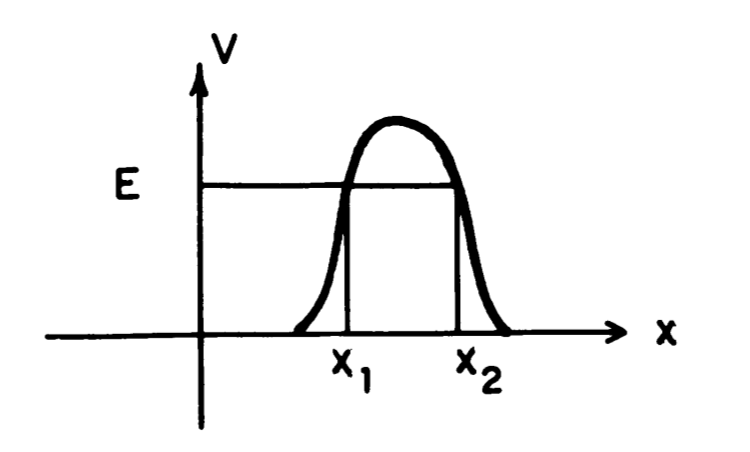
\includegraphics[width=0.6\textwidth]{instantonfig1.jpeg}
    \caption{ \label{instantonfig1}}
  \end{figure}

我们都知道这个跃迁振幅服从WKB公式
\begin{equation}
    \bigl\lvert T(E)\bigr\rvert =\exp\biggl(-\frac{1}{\hbar}\int_{x_{1}}^{x_{2}}\dif x\: \sqrt{2(V-E)}\biggr)[1+O(\hbar)] \:, \label{instanton1.7}
\end{equation}
其中$x_{1}$和$x_{2}$使得这个区域内的$V(x)$大于$E$. 
\begin{tcolorbox}
    一个非常简单的解释: 波函数可以近似写为$\exp(\mi p x/\hbar)$, 而$E=\frac{1}{2}p^{2}+V$, 所以在$E<V$时, $p=\mi\sqrt{2(V-E)}$, 波函数指数衰减.
\end{tcolorbox}
然而, 这个势垒隧穿在微扰论的任何阶都没有看到, 这是因为方程\eqref{instanton1.7}比$\hbar$的任意幂次都衰减的快, 因此也就比$g$的任意幂次都衰减得快.

在量子场论中, 尤其是量子色动力学中, 有类似于量子力学中的隧穿现象的效应, 这也就是所谓的瞬子.

{\heiti{符号说明}}: 时空特征是$({+}{-}{-}{-})$, $x^{0}$是时间坐标, $g_{\mu\nu}$是时空度规, $x^{4}=-\mi x^{0}$是到欧几里得时空的延拓.

\section{粒子力学中的瞬子和回弹} \label{instanton:sec2}

\subsection{欧几里得泛函积分} \label{instanton:sec2.1}

在本节我们继续处理单位质量的无自旋粒子在一维势下运动的理论:
\begin{equation}
    H = \frac{p^2}{2} + V(x) \:. \label{instanton2.1}
\end{equation}
这是一个量子力学问题, 但我们不采用处理这类问题的标准方法, 而是容易推广到量子场论的方法.

我们的基本工具是Feynman历史求和的欧几里得版:
\begin{equation}
    \langle x_{f} \vert \me^{-HT/\hbar} \vert x_{i}\rangle =N \int [\dif x]\, \me^{-S/\hbar} \:. \label{instanton2.2}
\end{equation}
方程\eqref{instanton2.2}左边的$\lvert x_{i}\rangle$和$\lvert x_{f}\rangle$是位置本征态, $H$是哈密顿量, 而$T$是一个正数. 利用能量本征态
\begin{equation}
    H\vert n \rangle = E_{n} \vert n\rangle \label{instanton2.3}
\end{equation}
展开方程\eqref{instanton2.2}左边, 那么就有
\begin{equation}
    \langle x_{f} \vert \me^{-HT/\hbar} \vert x_{i}\rangle 
    = \sum_{n}\me^{-E_{n}T/\hbar}  \langle x_{f} \vert n\rangle \langle n \vert x_{i}\rangle  \:. \label{instanton2.4}
\end{equation}
这个展开在大$T$时的领头项给出了能量最低的本征态的能量和波函数.

在方程\eqref{instanton2.2}右边, $N$是归一化常数, $S$是欧几里得作用量
\begin{equation}
    S=\int_{-T/2}^{T/2} \dif t\:\biggl[\frac{1}{2}\biggl(\frac{\dif x}{\dif t}\biggr)^{2}+V\biggr] \:, \label{instanton2.5}
\end{equation}
而$[\dif x]$代表对所有满足边界条件$x(-T/2)=x_{i}$和$x(T/2)=x_{f}$的函数$x(t)$积分. 更具体一些, 如果$\overline{x}$是满足边界条件的任意函数, 那么满足边界的一般函数可以写成
\begin{equation}
    x(t)=\overline{x}(t)+\sum_{n}c_{n}x_{n}(t) \:, \label{instanton2.6}
\end{equation}
其中$x_{n}$是在边界处为零的实正交函数完备集,
\begin{subequations}\label{instanton2.7}
    \begin{gather}
        \int_{-T/2}^{T/2} \dif t\: x_{n}(t)x_{m}(t) = \delta_{nm} \:, \label{instanton2.7a} \\
        x_{n}(\pm T/2)=0 \:.  \label{instanton2.7b}
    \end{gather}
\end{subequations}
这样, 测度就定义成
\begin{equation}
    [\dif x] = \prod_{n} (2\pi\hbar)^{-1/2} \dif c_{n} \:. \label{instanton2.8}
\end{equation}
(这里的归一化常数$N$依赖于测度的定义, 但是归一化常数会抵消, 所以不需要它的准确定义.)

方程\eqref{instanton2.2}右边可以用半经典(小$\hbar$)极限计算. 在这个情况下, 泛函积分由$S$的稳定点主导. 简单起见, 我们假定只有一个这样的稳定点, 我们将其记为$\overline{x}$, 它满足牛顿方程
\begin{equation}
    \frac{\delta S}{\delta x}\biggr\vert_{x=\overline{x}} = 
    -\frac{\dif^{2}\overline{x}}{\dif t^{2}} + V'(\overline{x}) = 0 \label{instanton2.9}
\end{equation} 
其中加撇号代表对$x$的导数. 更进一步, 我们令$x_{n}$是$S$在$\overline{x}$处的二阶变分导数的本征函数,
\begin{equation}
    -\frac{\dif^{2} x_{n}}{\dif t^{2}} + V''(\overline{x})x_{n} = \lambda_{n}x_{n} \:. \label{instanton2.10} 
\end{equation}
那么, 在小$\hbar$极限下, 这个积分变成高斯积分的乘积, 所以有
\begin{align}
    \langle x_{f} \vert \me^{-HT/\hbar} \vert x_{i}\rangle 
   & = N \me^{-S(\bar{x})/\hbar}\prod_{n}\lambda_{n}^{-1/2}[1+O(\hbar)] \nonumber \\
   &= N \me^{-S(\bar{x})/\hbar}\Bigl[\det\bigl(-\partial_{t}^{2}+V''(\overline{x})\bigr)\Bigr]^{-1/2}[1+O(\hbar)] \:. \label{instanton2.11}
\end{align}
如果有数个稳定点, 一般需要求和.
\begin{tcolorbox}
    这里解释一下方程\eqref{instanton2.10}和\eqref{instanton2.11}, 在$\overline{x}$附近展开$S$, 并设微扰为$\eta$, 那么
    \begin{align*}
        \delta S&= S(\overline{x}+\eta)-S(\overline{x}) 
        = \int \dif t\, \Bigl(\tfrac{1}{2}\bigl(\dot{\overline{x}}+\dot{\eta}\bigr)^{2}+V(\overline{x}+\eta)-\tfrac{1}{2}\dot{\overline{x}}^{2}-V(\overline{x})\Bigr) \\
        &=\int \dif t\,\Bigl(\dot{\overline{x}}\dot{\eta}- V'(\overline{x})\eta+\tfrac{1}{2}\dot{\eta}^{2}+\tfrac{1}{2}V''(\overline{x})\eta^{2}+O(\eta^{2})\Bigr)
        =\frac{1}{2}\int \dif t\, \eta(-\partial_{t}^{2}+V'')\eta
    \end{align*}
在最后一个等号这里使用了牛顿方程\eqref{instanton2.9}, 分部积分并忽略了$\eta$的高阶项. 

用$(-\partial_{t}^{2}+V'')$的本征函数完备集$\{x_{n}\}$展开$\eta=\sum c_{n}x_{n}$, 利用方程\eqref{instanton2.7}就得到了
\begin{equation*}
    \delta S= \frac{1}{2} \lambda_{n}c_{n}^{2}
\end{equation*}
那么
\begin{align*}
    N \int [\dif x]\, \me^{-S/\hbar}&=N \me^{-S(\overline{x})/\hbar} \int [\dif x]\, \me^{-\delta S/\hbar} \\
    &=N \me^{-S(\overline{x})/\hbar} \int \prod_{n} (2\pi\hbar)^{-1/2} \dif c_{n}\:\me^{-\frac{1}{2} \lambda_{n}c_{n}^{2}/\hbar}
    =N \me^{-S(\overline{x})/\hbar}\prod_{n} \lambda_{n}^{-1/2} .
\end{align*}
\end{tcolorbox}

根据方程\eqref{instanton2.9}, 能量是
\begin{equation}
    E=\frac{1}{2}\biggl(\frac{\dif\overline{x}}{\dif t}\biggr)^{2} - V(\overline{x})
\end{equation}
这可以用来决定方程\eqref{instanton2.9}的解的定性性质.

\begin{figure}[h]
    \centering
    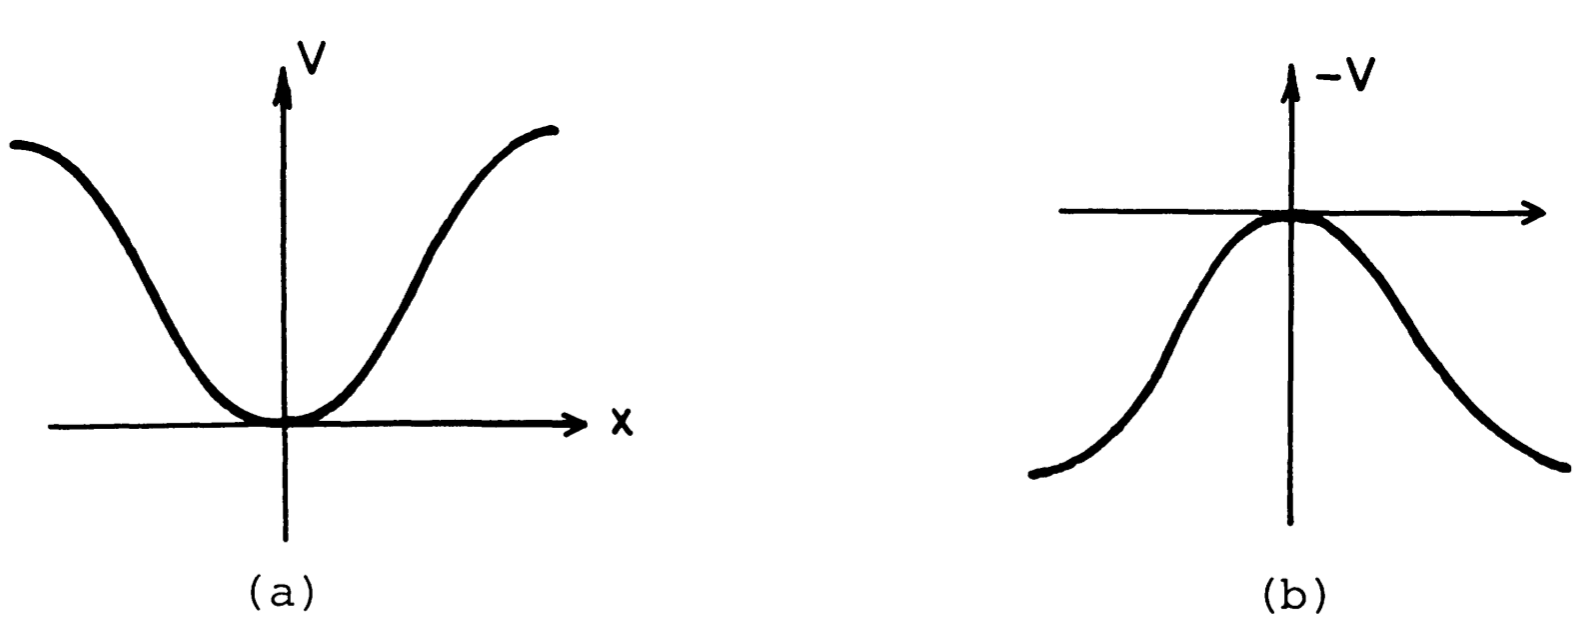
\includegraphics[width=0.8\textwidth]{instantonfig2.jpeg}
    \caption{ \label{instantonfig2}}
  \end{figure}
作为一个简单例子, 考虑图\ref{instantonfig2}(a)中的势能. 选择$x_{i}=x_{f}=0$. 方程\eqref{instanton2.9}满足边界条件的解显然是
\begin{equation}
    \overline{x}=0 . \label{instanton2.13}
\end{equation}
对于这个解, $S(\overline{x})=0$. 那么, 从方程\eqref{instanton2.11}
\begin{equation}
    \langle 0 \vert \me^{-HT/\hbar} \vert 0\rangle = 
    N[\det(-\partial_{t}^{2}+\omega^{2})]^{-1/2}[1+O(h)] \:, \label{instanton2.14}
\end{equation}
其中
\begin{equation}
    \omega^{2}=V''(0) \:. \label{instanton2.15}
\end{equation}

可以证明, 对于很大的$T$,
\begin{equation}
    N[\det(-\partial_{t}^{2}+\omega^{2})]^{-1/2} \simeq \biggl(\frac{\omega}{\pi\hbar}\biggr)^{1/2}\me^{-\omega T/2}.  \label{instanton2.16}
\end{equation}
根据方程\eqref{instanton2.4}, 基态能量是
\begin{equation}
    E_{0}=\frac{1}{2}\omega\hbar[1+O(\hbar)] \:. \label{instanton2.17}
\end{equation}
同理, 基态粒子处在原点的几率是
\begin{equation}
     \bigl\lvert \langle x{=}0 \vert n{=}0 \rangle \bigr\rvert^{2} =
     (\omega/\pi\hbar)^{1/2}[1+O(\hbar)] .
\end{equation}

这些当然是正确的半经典结果. 在小$\hbar$极限下, 粒子处在位于原点的谐振子基态中, 能量就是谐振子的基态能量.

\begin{tcolorbox}[breakable]
    推导方程\eqref{instanton2.16}的两种方法:

    (1)蛮干法(Poor man's way): 求解如下微分方程
\[
 (-\partial_{t}^{2}+\omega^{2})f= \lambda_{n}f
\]
由于$f$要满足边界条件$f(\pm T/2)=0$, 所以$\lambda_{n}>\omega^{2}$, 并要满足
\[
 \sqrt{\lambda_{n}-\omega^{2}} = \frac{n\pi}{T}    
\]
那么根据方程\eqref{instanton2.11}, 
\begin{align*}
    [\det(-\partial_{t}^{2}+\omega^{2})]^{-1/2}
    =\prod_{n}\biggl(\frac{n^{2}\pi^{2}}{T^{2}}+\omega^{2}\biggr)^{-1/2}
\end{align*}
上式需要重整化, 除以一个不依赖于$\omega$的无限大常数$[\det(-\partial_{t}^{2})]^{-1/2}$, 得到
\begin{align*}
    [\det(-\partial_{t}^{2}+\omega^{2})]^{-1/2}&=\prod_{n}\Biggl(
        1+ \biggl(\frac{\omega T}{n\pi}\biggr)^{2}\Biggr)^{-1/2} \\
        &= \biggl(\frac{\sinh(\omega T)}{\omega T}\biggr)^{-1/2}
\end{align*}
在$T$很大时, $\sinh(\omega T)\simeq \me^{\omega T}$. 常数$N$可以通过考虑自由粒子来决定, 这里不再赘述.

(2) Coleman的方法, 根据定义
\[
\det(-\partial_{t}^{2}+W)=\prod_{n}\lambda_{n}    
\]
其中$\lambda_{n}$是算符$(-\partial_{t}^{2}+W)$的本征值, 那么$(-\partial_{t}^{2}+W-\lambda)$的本征值是$\lambda_{n}-\lambda$. 这样就有
\[
\frac{\det(-\partial_{t}^{2}+W^{(1)}-\lambda)}{\det(-\partial_{t}^{2}+W^{(2)}-\lambda)}  = \frac{\psi_{\lambda}^{(1)}(T/2)}{\psi_{\lambda}^{(2)}(T/2)}  .
\]
这里$\psi$满足
$(-\partial_{t}^{2}+W^{(i)})\psi_{\lambda}^{(i)}=\lambda \psi_{\lambda}^{(i)}$以及边界条件$\psi_{\lambda}(-T/2)=0$和$\dot{\psi}_{\lambda}(-T/2)=1$. 显然$\psi_{\lambda}^{(i)}$只有$\lambda=\lambda_{n}$时满足边界条件$\psi_{\lambda}^{(i)}(\pm T/2)=0$. 将上式左右两边视为$\lambda$的函数, 那么左右两边就有相同的零点和极点, 所以相等.

由此可得
\[
    \frac{\det(-\partial_{t}^{2}+W)}{\psi_{0}(T/2)} =\text{常数} = \pi\hbar N^{2} 
\]
其中$N$是一个常数. (这也是Coleman对$N$的定义.) 对于$W=\omega^{2}$, 可以解出
\[
\psi_{0}=\omega^{-1} \sinh \omega(t+T/2)\:,   
\]
进而也就得到了方程\eqref{instanton2.16}

\end{tcolorbox}


\subsection{双井与瞬子} \label{instanton:sec2.2}

我们现在转向不那么平庸的问题, 图\ref{instantonfig3}(a)所示的双井. 假定势是偶函数, $V(x)=V(-x)$, 它的最小值点记为$\pm a$. 选择一个常数, 使得$V$的最小值是0, 并将$V''(\pm a)$记为$\omega^{2}$.
\begin{figure}[h]
    \centering
    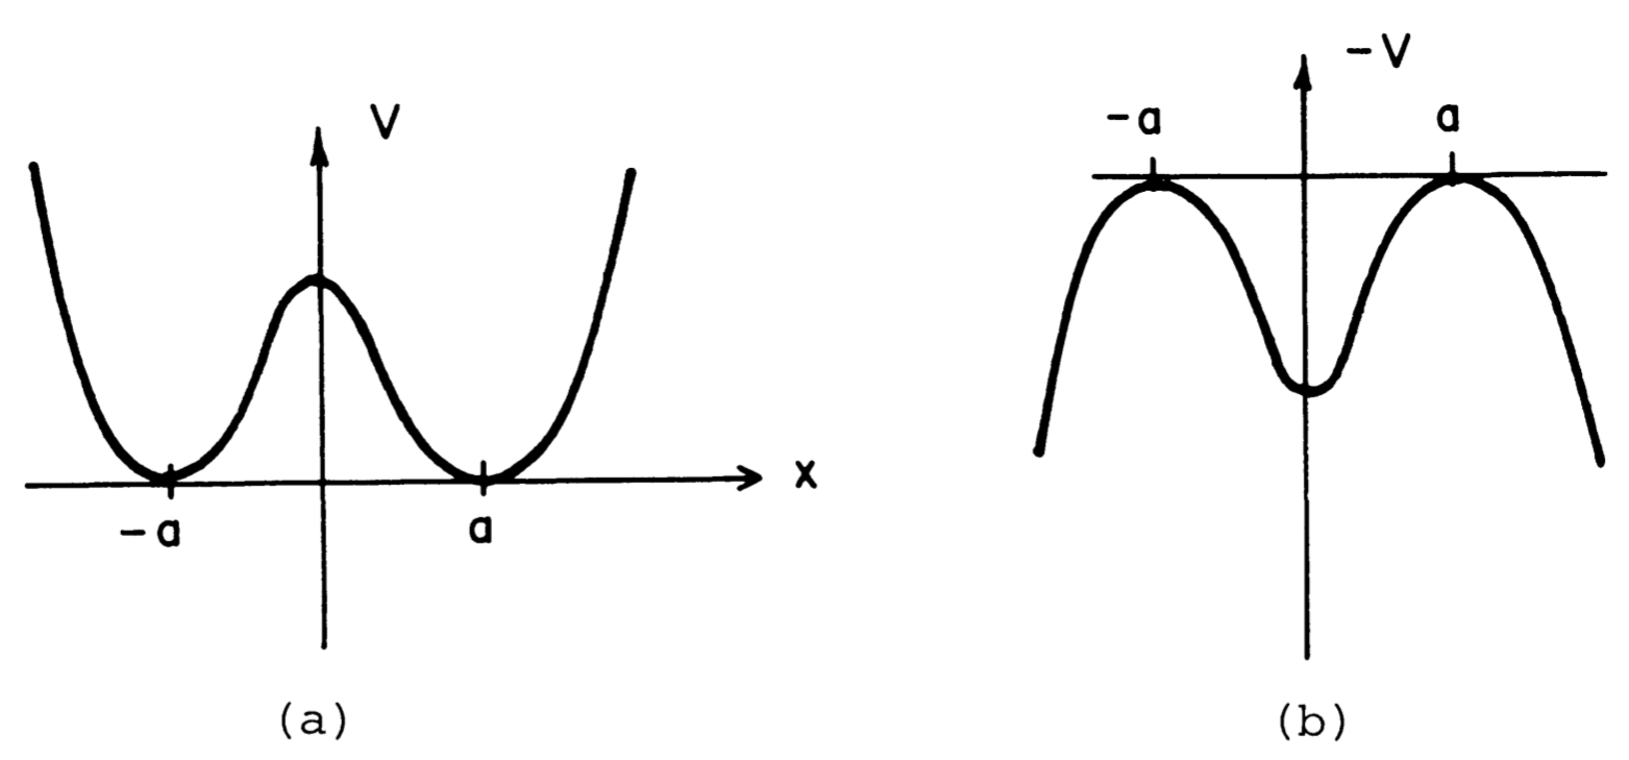
\includegraphics[width=0.8\textwidth]{instantonfig3.pdf}
    \caption{ \label{instantonfig3}}
\end{figure}

我们将尝试计算
\begin{subequations}
    \begin{align}
        \langle {-}a \vert \me^{-HT} \vert {-}a \rangle &= \langle a \vert \me^{-HT} \vert a \rangle \:, \label{instanton2.19a}\\ 
        \langle a \vert \me^{-HT} \vert {-}a \rangle &= \langle {-}a \vert \me^{-HT} \vert a \rangle \:,\label{instanton2.19b}
    \end{align}
\end{subequations}
方法是通过半经典极限方程\eqref{instanton2.11}来近似泛函积分. 和前面一样, 先求解与边界条件相容的经典欧几里得运动方程, \eqref{instanton2.9}. 

当然, 两个这样的解是粒子待在两个井底(或者说图\ref{instantonfig3}(b)的两个山顶). 然而还有另一种有趣的解, 在$-T/2$时待在其中一个山顶, 然后在$T/2$时跑到另一个山顶.
由于我们最后会把$T$取为无穷大, 我们将专注于这个极限下的解形式, 即粒子在无穷远的过去从一个山顶离开, 然后在无穷远的未来达到另一个山顶. 在这个情况下, 运动方程的解的能量为零; 
所以
\begin{equation}
    \dif x/\dif t =\sqrt{2V}. \label{instanton2.20}
\end{equation}
等效地有
\begin{equation}
    t= t_{1}+\int_{0}^{x}\dif x' \: (2V)^{-1/2} \:, \label{instanton2.21}
\end{equation}
其中$t_{1}$是积分常数, $x(t_{1})$为零.

\begin{figure}[h]
    \centering
    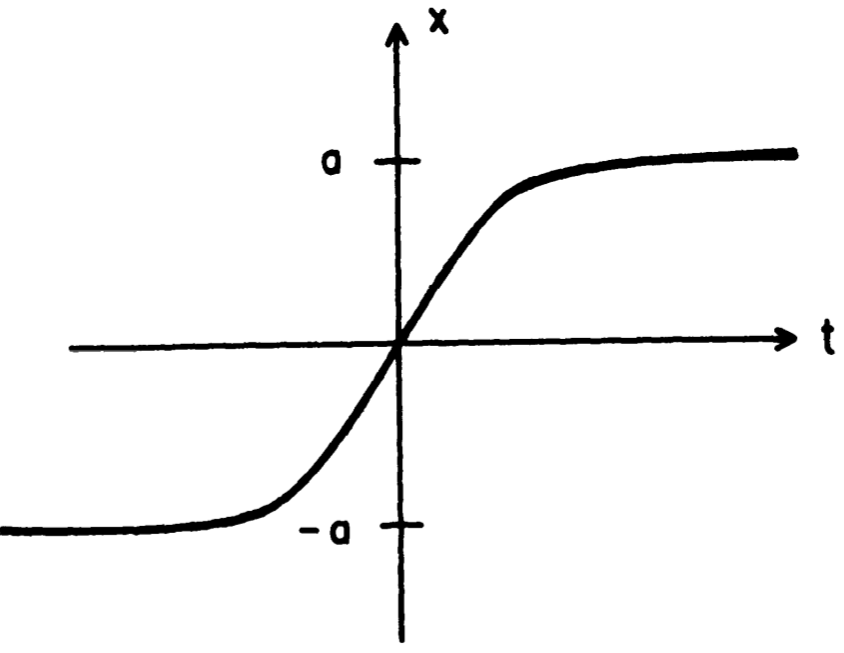
\includegraphics[width=0.5\textwidth]{instantonfig4.jpeg}
    \caption{ \label{instantonfig4}}
  \end{figure}

解的图示参看图\ref{instantonfig4}; 它被称为``中心在$t_{1}$的瞬子''. 瞬子这一词汇是't Hooft发明的. 灵感来源于它们的数学结构十分类似于所谓的孤子(solitons)或鼓包(lump), 
经典场论的类粒子解: 因此称为``-子''. 然而, 不像鼓包, 它们在时间(尽管是欧几里得时间)中是局域的: 因此是``瞬-''. 由于相同的原因, Polyakov称其为``赝粒子(pseudoparticle)'', 也见于文献.

当然, 我们可以也可以构建从$a$到${-}a$的解, 将方程\eqref{instanton2.21}中的$t$换为$-t$即可; 它们被称为``反瞬子''.

这些解有两个很重要的性质:
\begin{enumerate}
    \item 从方程\eqref{instanton2.20}可以导出瞬子(或反瞬子)作用量的一个简单表达式
    \begin{equation}
        S_{0}=\int \dif t\:\bigl[\tfrac{1}{2}\dot{x}^{2}+V\bigr] =\int \dif t \: \dot{x}^{2} = \int_{-a}^{a}\dif x\:\sqrt{2V} \:. \label{instanton2.22}
    \end{equation}
    注意这与势垒隧穿公式\eqref{instanton1.7}中出现的积分相同. 我们会在后面看到这不是个巧合.
    \item 对于大$t$, $x$趋于$a$, 方程\eqref{instanton2.20}可以近似为
    \begin{equation}
        \dot{x} = \omega(a-x) \:. \label{instanton2.23}
    \end{equation}
    因此, 对于大$t$,
    \begin{equation}
        (a-x) \propto \me^{-\omega t} \:. \label{instanton2.24}
    \end{equation}
    因此瞬子是一个非常定域的物体, 它的尺寸大约是$1/\omega$阶的.
\end{enumerate}

这是十分重要的, 因为这意味着: 当$T$很大时, 瞬子和反瞬子不仅是运动方程的近似解; 相距甚远的瞬子和反瞬子串联而成的场构型也是近似解. 

泛函积分将通过对所有这样的构型求和计算, 其中每个构型有$n$个物体(瞬子或反瞬子), 中心处在$t_{1},\ldots,t_{n}$, 其中
\begin{equation}
    T/2>t_{1}>\cdots>t_{n}>-T/2\:. \label{instanton2.25}
\end{equation}

图\ref{instantonfig5}展示了这样一个构型. $T$相比于瞬子尺寸要大很多; 因此图\ref{instantonfig4}的光滑曲线在图5的尺度上就变成了尖锐的跃变. 

\begin{figure}[h]
    \centering
    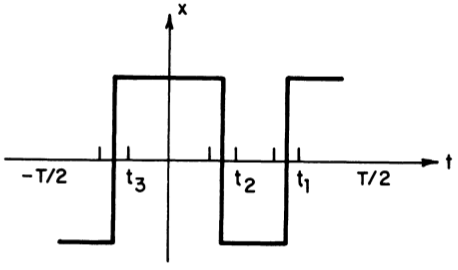
\includegraphics[width=0.6\textwidth]{instantonfig5.jpeg}
    \caption{ \label{instantonfig5}}
  \end{figure}

现在是计算:
\begin{enumerate}
    \item 对于$n$个相距甚远的物体, $S$就是$n S_{0}$. 要考虑到作用量在指数上.
    \item 泛函行列式的计算需要一些技巧. 我们把时间演化算符$\me^{-HT}$视为图\ref{instantonfig5}中时间轴上垂直线所标出的点之间的演化算符的乘积. 
    要不是存在含有瞬子和反瞬子的小区间, $V''$在整个时间上等于$\omega^{2}$, 因此我们所获得的结果与\ref{instanton:sec2.1}节中的单井势的结果相同, 
    \begin{equation}
        \biggl(\frac{\omega}{\pi\hbar}\biggr)^{1/2} \me^{-\omega T/2} \:. \label{instanton2.26}
    \end{equation}
    含有瞬子和反瞬子的小区间修正了这个公式. 因此我们得到
    \begin{equation}
        \biggl(\frac{\omega}{\pi\hbar}\biggr)^{1/2} \me^{-\omega T/2}K^{n} \:. \label{instanton2.27}
    \end{equation}
    其中$K$可以通过计算只有一个瞬子的情况得到.
    \item 我们必须要对瞬子中心所处的位置的积分:
    \begin{equation}
        \int_{-T/2}^{T/2} \dif t_{1}\int_{-T/2}^{t_{1}} \dif t_{2} \cdots \int_{-T/2}^{t_{n-1}} \dif t_{n} 
        =T^{n}/n! \:. \label{instaton2.28}
    \end{equation}
    \item 我们无法自由地分配瞬子和反瞬子. 例如, 如果我们从${-}a$出发, 那么第一个遇到的物体必然是瞬子, 下一个必然是反瞬子, 以此类推. 
    更进一步, 如果我们最后返回${-}a$, $n$必须是偶数. 同样, 如果我们最后停到了$a$, $n$必须是奇数. 
\end{enumerate}

因此,
\begin{equation}
    \langle{-}a\vert \me^{-HT/\hbar} \vert {-a}\rangle 
    =\biggl(\frac{\omega}{\pi\hbar}\biggr)^{1/2} \me^{-\omega T/2} 
    \sum_{\text{even }n} \frac{\bigl(K\me^{-S_{0}/\hbar}T\bigr)^{n}}{n!}[1+O(\hbar)] \:, \label{instanton2.29}
\end{equation}
而$\langle a\vert \me^{-HT/\hbar} \vert {-a}\rangle $由只对奇数$n$求和的相同表达式给出. 这些求和是平庸的:
\begin{equation}
    \langle \pm a\vert \me^{-HT/\hbar} \vert {-a}\rangle 
    =\frac{1}{2}\biggl(\frac{\omega}{\pi\hbar}\biggr)^{1/2} \me^{-\omega T/2}
    \Bigl[\exp\bigl(K\me^{-S_{0}/\hbar}T\bigr)\pm \exp\bigl(-K\me^{-S_{0}/\hbar}T\bigr)\Bigr] 
    \:, \label{instanton2.30}
\end{equation}
(从现在起将省略因子$[1+O(\hbar)]$.)

与方程\eqref{instanton2.4}比较, 我们现在有两种能量最底态, 其能量是
\begin{equation}
    E_{\pm} = \tfrac{1}{2}\hbar\omega \pm \hbar K \me^{-S_{0}/\hbar} \:. \label{instanton2.31}
\end{equation}
如果我们把这些本征态记为$\lvert + \rangle$和$\lvert - \rangle$, 我们看到
\begin{equation}
    \bigl \lvert \langle + \vert {\pm} a \rangle \bigr \rvert^{2} = \bigl \lvert \langle - \vert {\pm} a \rangle \bigr \rvert^{2} 
    =\langle a\vert -\rangle \langle - \vert {-}a\rangle =-\langle a\vert +\rangle \langle + \vert {-}a\rangle 
    =\frac{1}{2} \biggl(\frac{\omega}{\pi\hbar}\biggr)^{1/2} \:. \label{instanton2.32}
\end{equation}
当然, 它们是预期的结果: 能量本征态是中心在两个井底的谐振子态在空间上为偶或为奇的组合; 两个能量本征态的简并只被势垒隧穿破坏了(因此能量差正比于势垒隧穿因子$\me^{-S_{0}/\hbar}$), 而能量较低的态, 即我们记为$\lvert -\rangle$的那个, 在空间上为偶的组合. \\
\begin{remark}
设$\vert + \rangle= (m_{+}\lvert 0_{+}\rangle+n_{+}\lvert 0_{-}\rangle)/\sqrt{2}$和$\vert - \rangle= (m_{-}\lvert 0_{+}\rangle+n_{-}\lvert 0_{-}\rangle)/\sqrt{2}$, 其中$\lvert 0_{\pm}\rangle$是中心分别处在$\pm a$的谐振子态. 方程\eqref{instanton2.32}给出$m_{+}=-n_{+}$和$m_{-}=n_{-}$, 以及它们的范数为1.
\end{remark}

下个任务是计算$K$. 在计算之前, 我们先对所做的事情做一些评论:
\begin{enumerate}
    \item 实际上我们没有权利在方程\eqref{instanton2.31}中保留第二项. 不仅是因为它指数式小于第一项, 它也指数式得小于对第一项的未知$O(\hbar^{2})$修正. 然而这是对能量差$E_{+}-E_{-}$的领头阶修正; 一个更加严格的做法是仅在能量差的表达式中保留这一项, 而在单个能量的表达式中略去它.
    \item 我们的近似基于瞬子和反瞬子相距甚远的假定. 作为一个自洽性检验, 我们应该验证最后结果的主要部分来自于这样的构型. 
    
    这个检验很容易做. 对于固定的$x$, 指数系数$\sum x^{n}/n!$中的项随着$n$的增长而增长直到$n$到达$x$的量级, 在这之后, 开始快速衰减. 对方程\eqref{instanton2.29}中的求和应用这个性质, 我们看到重要的项是那些
    \begin{equation}
        n \lesssim KT \me^{-S_{0}/\hbar} \label{instanton2.33}
    \end{equation}
    的项. 这就是说, 对于小$\hbar$, 求和中重要的项是那些瞬子和反瞬子密度$n/T$是指数量级小数的项, 因此平均间隔非常大. 注意到这个平均间隔$K\me^{-S_{0}\hbar}$实际上独立于$T$; 我们的近似实际上是小$\hbar$近似; 只要$T$足够大, 这个条件就独立于$T$而成立.

    瞬子相距甚远这个近似被称为稀薄气体近似.
    \item 最后进一步解释下$S$的近似稳相点这个概念. 我们先来看单变量积分,
    \begin{equation}
        I=\int_{0}^{T} \dif t\: \me^{-S(t)/\hbar} \:, \label{instanton2.34}
    \end{equation}
    其中$S$是$t$的单调递减函数, 它的渐进值是$S(\infty)$. 因此这个被积函数在积分区域中没有稳相点. 然而对于小$\hbar$和大$T$, 很容易找到这个积分的如下近似形式
    \begin{equation}
        I\approx T \me^{-S(\infty)/\hbar} \:. \label{instanton2.35}
    \end{equation}
    大概地讲, 这个积分被无穷远处的稳相点所主导. 将这个现象推广到多维积分是直接的: 我们假定被积函数的图像有某种波谷; 沿着谷底的线会随着我们趋于无穷远而变平. 换言之, 在高维空间中有一条线, 使得被积函数在垂直于线的方向上在该线所处的位置达到最小值, 并在沿着这条线趋于无穷远时达到某个近似值. 当然这个线本身可以推广至超平面. ``近似稳相点''实际上就是这样的情况; 瞬子和反瞬子的所在就是沿着谷底的变量; $S$仅在它们趋于无穷远处变得稳定(并等于$nS_{0}$).
\end{enumerate}
\vspace{0.5cm}
现在我们来计算$K$.

我们现在必须要研究本征方程\eqref{instanton2.10}, 其中$\overline{x}$是单瞬子. 由于时间平移不变性, 这个方程必然有一个本征值为零的本征函数,
\begin{equation}
    x_{1} = S_{0}^{-1/2} \dif \overline{x}/\dif t \:. \label{instanton2.36}
\end{equation}
(归一化因子来自于方程\eqref{instanton2.22}.)
\begin{tcolorbox}
    我们稍微解释一下函数\eqref{instanton2.36}的来源. 这里的时间平移性是指: 当时间$T$是无穷时, 无论单瞬子$\overline{x}$的中心在哪, 作用量$S(\bar{x})$都是相同的. 设中心在$t_{1}$的单瞬子为$\bar{x}(t-t_{1})$, 那么对于两个相距很近的单瞬子, 我们就有
    \begin{equation*}
        0=\delta S= S[\overline{x}(t-t_{1}-\Delta t_{1})]-S[\overline{x}(t-t_{1})]=\frac{1}{2}\int \dif t\, \eta(-\partial_{t}^{2}+V'')\eta
    \end{equation*} 
    其中$\eta=\overline{x}(t-t_{1}-\Delta t_{1})-\overline{x}(t-t_{1})=-\Delta t_{1} \, \dot{\overline{x}}(t-t_{1})$. 由于算符$(-\partial_{t}^{2}+V'')$没有非负本征值, 所以这个$\eta$肯定是这个算符本征值为零的本征函数. 归一化因子是要求
    \begin{equation*}
        \int \dif t\: x_{1}^{2} =1 
    \end{equation*}
    得到的, 其中用到了方程\eqref{instanton2.22}.
\end{tcolorbox}
如果我们要想对方程\eqref{instanton2.6}中的相应展开系数$c_{1}$积分, 我们会遇到无穷大, 但这个积分实际上已经在对瞬子中心的积分\eqref{instaton2.28}中做过了. 
原因是, 瞬子$\overline{x}(t)$的中心移动所产生的微扰是:
\begin{equation}
    \eta =\dot{\overline{x}} \Delta t_{1} \:. \label{instanton2.37}
\end{equation}
而这造成了本征函数展开系数的扰动
\begin{equation}
    \eta =x_{1}\Delta c_{1} \:. \label{instanton2.38}
\end{equation}
因此,
\begin{equation}
    (2\pi\hbar)^{-1/2} \dif c_{1} = (S_{0}/2\pi\hbar)^{1/2} \dif t_{1} \:.
\end{equation}

因此, 在计算泛函行列式时, 我们应该排除零本征值, 但我们应该该$K$引入因子$(S_{0}/2\pi\hbar)^{1/2}$. 因此, 单瞬子对这个跃迁元的贡献是
\begin{equation}
    \langle a \vert \me^{-HT} \vert {-}a\rangle _{\text{one inst.}} =N T  (S_{0}/2\pi\hbar)^{1/2} \me^{-S_{0}/\hbar}
    \bigl(\det\nolimits'[-\partial_{t}^{2}+V''(\overline{x})]\bigr)^{-1/2} \:, \label{instanton2.40}
\end{equation}
其中$\det'$是指在计算行列式时已经排除了零本征值. 与\eqref{instanton2.29}相比较, 我们得到
\begin{equation}
    K= (S_{0}/2\pi\hbar)^{1/2} \Biggl\lvert \frac{\det(-\partial_{t}^{2}+\omega^{2})}{\det'\bigl(-\partial_{t}^{2}+V''(\overline{x})\bigr)} \Biggr\rvert^{1/2} \:.
\end{equation}

一些注解:
\begin{enumerate}
    \item 为了真的把所有元素缝合在一起, 我们应该证明我们所得到的能级分裂公式与通过传统波动力学方法得到的相同. 这个会在附录中解释.
    \item 我们现在来论述算符$-\partial_{t}^{2}+V''(\overline{x})$的本征值都是非负的. 这个算符是Schr\"{o}dinger方程中的算符, 本征值越大的本征函数拥有更多的节点(零点), 或者更多的波峰波谷(这样本征函数的频率也就越高). 瞬子是单调增函数, 它的导数没有节点, 再加上这个导数是这个算符本征值为零的本征函数. 证毕.
    \item $K$正比于$\hbar^{-1/2}$. 这个因子来自于时间平移不变性产生的零模. 稍后我们会分析拥有更大对称群的理论, 对于这些理论, 瞬子有多个这样的零模. 显然, 每个零模都会给一个$\hbar^{-1/2}$因子. 这种对$\hbar$的幂次计数的规则将起到重要作用, 正如第\ref{instanton:sec1}节所解释的那样, 对$\hbar$的幂次计算等同于对耦合常数的幂次计数.
\end{enumerate}

\subsection{周期势}

我们来考虑如图\ref{instantonfig6}(a)所示的周期势. (方便起见, $V$的最小值点被取成了整数.) 如果忽略势垒隧穿, 能量本征态就是无限多个简并态, 每个都集中在某个井底. 
势垒隧穿将单个本征值变成了连续的本征值带; 真正的能量本征态势单位平移的本征态, Bloch波. 我们现在看一下如何用瞬子方法推导这个旧结果.
\begin{figure}[h]
    \centering
    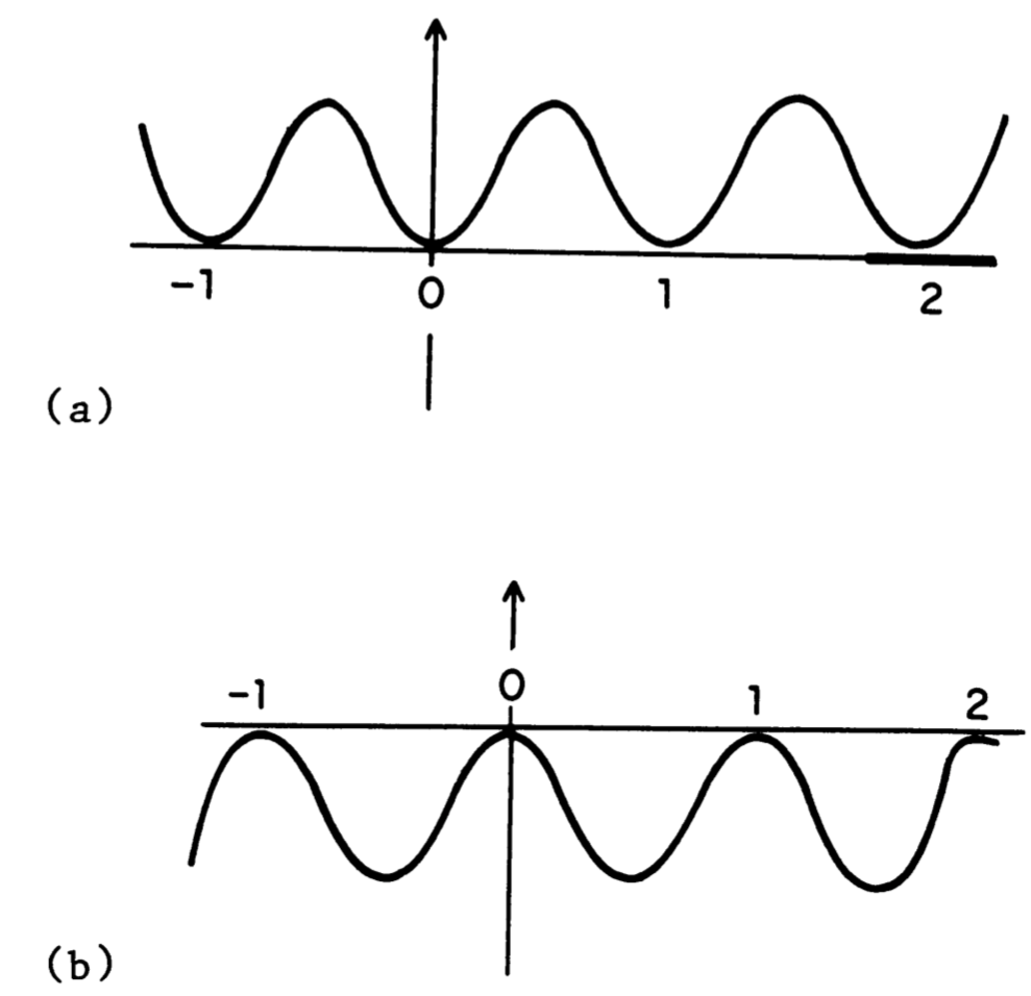
\includegraphics[width=0.5\textwidth]{instantonfig6.pdf}
    \caption{ \label{instantonfig6}}
  \end{figure}

我们从图\ref{instantonfig6}(b)中可以看到, 这里的瞬子和前面的很像. 唯一新的地方是瞬子现在可以从任何初始位置$x=j$出发, 然后去往下一个$x=j+1$. 反瞬子则是从$x=j$到$x=j-1$. 
其余的和之前相同.

因此, 当做稀薄气体求和时, 我们可以在实轴上分布瞬子和反瞬子, 不再有瞬子和反瞬子交替分布这样的约束. 当然, 当我们沿着线行进时, 
每个瞬子或反瞬子都必须从它的前任者的终点出发. 更进一步, 瞬子的总数减去反瞬子的总数必须等于初始位置本征态和终末位置本征态的$x$的变化.

因此我们得到
\begin{equation}
    \langle j_{+} \vert \me^{-HT/\hbar} \vert j_{-} \rangle = \biggl( \frac{\omega}{\pi\hbar}\biggr)^{1/2} \me^{-\omega T/2}
    \sum_{n=0}^{\infty}\sum_{\overline{n}=0}^{\infty} \frac{1}{n!\overline{n}!} \Bigl( K\me^{-S_{0}/\hbar}T\Bigr)^{n+\overline{n}}
    \delta_{n-\overline{n}\,,\,j_{+}-j_{-}} \label{instanton2.42}
\end{equation}
其中$n$是瞬子总数而$\overline{n}$是反瞬子总数. 如果我们使用恒等式
\begin{equation}
    \delta_{a,b}= \int_{0}^{2\pi} \frac{\dif \theta}{2\pi} \:\me^{\mi\theta(a-b)} \:, \label{instanton2.43}
\end{equation}
求和就变成了两个独立的指数级数, 我们发现
\begin{equation}
    \langle j_{+} \vert \me^{-HT/\hbar} \vert j_{-} \rangle = \biggl( \frac{\omega}{\pi\hbar}\biggr)^{1/2} \me^{-\omega T/2}
    \int_{0}^{2\pi}  \frac{\dif \theta}{2\pi} \:\me^{\mi\theta(a-b)}\exp\Bigl[2KT\cos\theta \me^{-S_{0}/\hbar}\Bigr] \:. \label{instanton2.44}
\end{equation}

因此我们得到了用角度$\theta$标记的连续能量本征态. 能量本征值是
\begin{equation}
    E(\theta) = \tfrac{1}{2}h\omega +2 hK \cos\theta \me^{-S_{0}/\hbar} \:. \label{instanton2.45}
\end{equation}
以及
\begin{equation}
    \langle \theta \vert j\rangle =\biggl( \frac{\omega}{4\pi^{3}\hbar}\biggr)^{1/4}  \me^{\mi j\theta} \:. \label{instanton2.46}
\end{equation}
这正是正确结果.

\subsection{非稳态与回弹}

\subsubsection*{伽利略戏仿\footnote{这里仿照了伽利略著作《关于托勒密和哥白尼两大世界体系的对话》的对话体形式, 本节中出现的沙格列陀(Sagredo)和萨尔维阿蒂(Salviati)正是此书中参与对话的两个主要人物, 名字取自伽利略的好友.}} 

\begin{figure}[h]
    \centering
    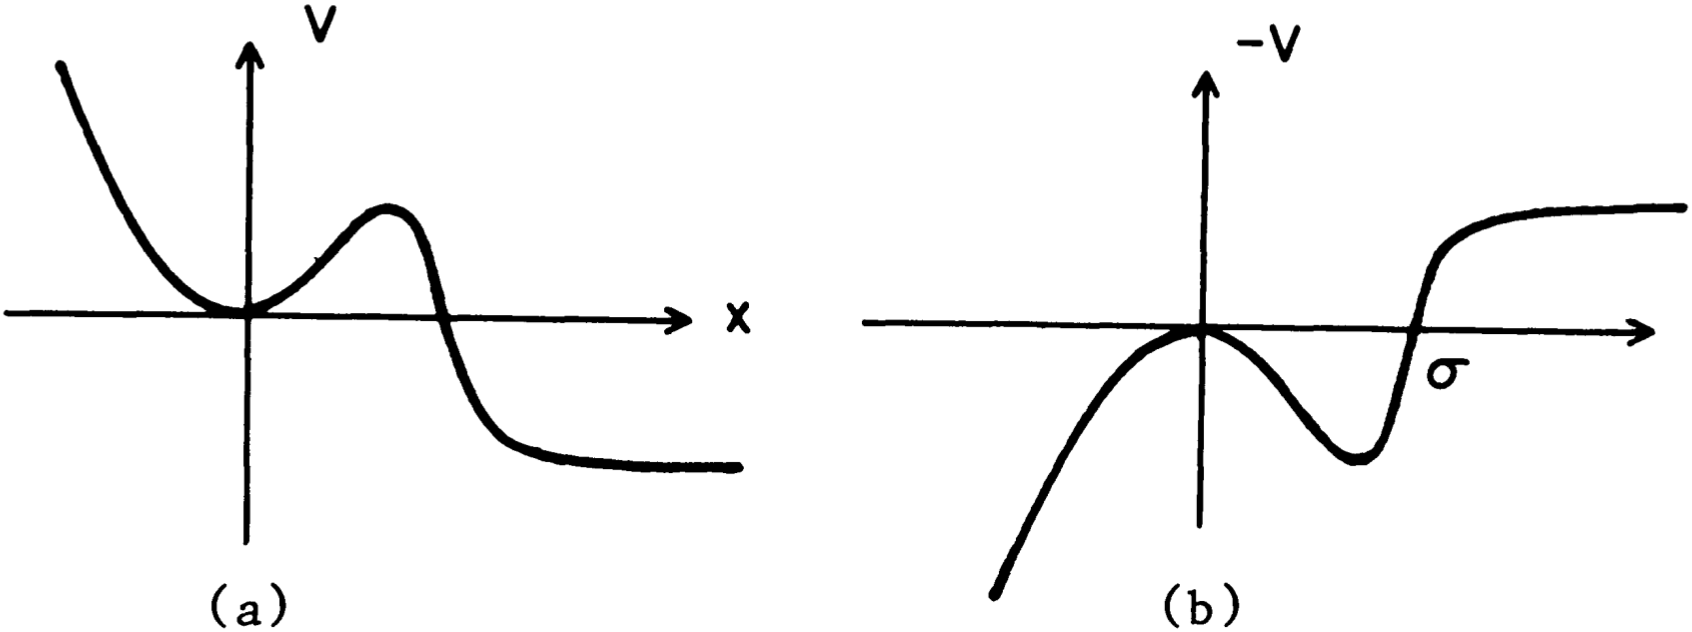
\includegraphics[width=0.7\textwidth]{instantonfig7.png}
    \caption{ \label{instantonfig7}}
  \end{figure}

\noindent {\kaishu{沙格列陀}}: 我想通过用瞬子方法研究图\ref{instantonfig7}(a)中的势以检查我对它们的理解. 如果我忽略势垒隧穿, 在半经典极限下, 这个势有一个处在井底的能量本征态. 我想计算势垒隧穿对这个态的能量的修正. 如果我把这个势上下颠倒(图\ref{instantonfig7}(b)), 我观察到经典运动方程有这样一个解: 粒子从$x=0$处的山顶出发,然后在经典转折点$\sigma$处反弹, 最后回到山顶(图\ref{instantonfig8}). 我们称这种运动为``回弹''(the bounce). 就像在研究双井势时对瞬子和反瞬子求和, 我将通过对相距甚远的回弹构型求和来计算$x=0$和$x=0$之间的跃迁矩阵元. 诚然, 除了对回弹的数目是奇是偶没有限制, 这个求和与双井势的情况相同(这里如何定义$S_{0}$、$\omega^{2}$等是显然的). 因此这里的指数级数是完整的, 而不是只有奇数项或偶数项, 这样就有
\begin{equation}
    \langle 0 \vert \me^{-HT/\hbar} \vert 0 \rangle =\biggl(\frac{\omega}{\pi\hbar}\biggr)^{1/2} \me^{-\omega T/2}
    \exp\bigl[KT \me^{-S_{0}/\hbar}\bigr] \:, \label{instanton2.47}
\end{equation}
而能量本征态是
\begin{equation}
    E_{0}=\tfrac{1}{2}\hbar\omega+\hbar K\me^{-S_{0}/\hbar} \:. \label{instanton2.48}
\end{equation}

\begin{figure}[h]
    \centering
    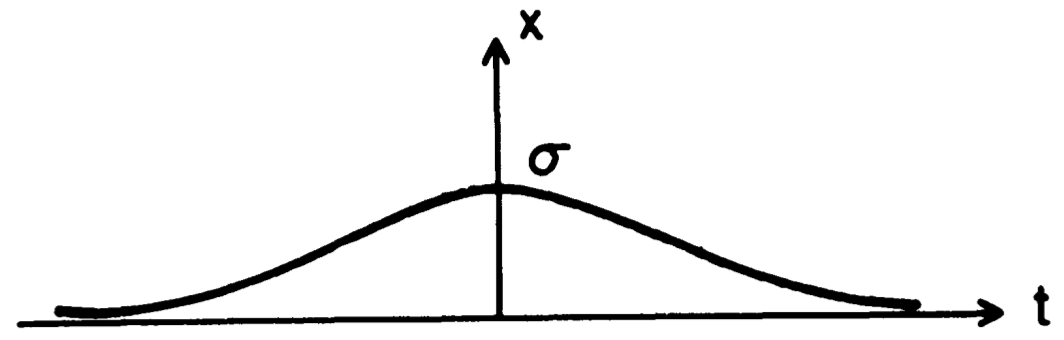
\includegraphics[width=0.5\textwidth]{instantonfig8.png}
    \caption{ \label{instantonfig8}}
  \end{figure}

\noindent {\kaishu{萨尔维阿蒂}}: 唉, 沙格列陀, 我恐怕你在三个地方出错了. 首先, 你所计算的项要远小于$\hbar^{2}$阶的项, 而你在计算过程中忽略了这样的项, 因此你没有理由保留它. 其次, 通过你的概述, 我看到这个回弹有个极大值; 而本征函数$x_{1}$正比于回弹的时间导数, 所以有一个节点. 因此它不是本征值最低的本征函数, 并且必然有一个本征值很低的无节点本征函数$x_{0}$, 这就是说, 必然有一个负本征值. $K$反比与本征值平方根之积, 因此是纯虚的. 最后, 你所研究的态由于势垒隧穿而变得不稳定, 因此你尝试计算的本征值不在哈密顿量的频谱中.

\noindent {\kaishu{沙格列陀}}: 你所说的都是正确的, 但我觉得你的批评也恰好指出了如何修正这个计算. 非稳态的能量有一个虚部; 因此只能期待$K$应该是纯虚的. 更进一步, 尽管我所计算的项相比于$E_{0}$的实部是可忽视的项, 但它是$E_{0}$虚部的领头贡献. 因此, 方程\eqref{instanton2.48}的修正版是
\begin{equation}
    \operatorname{Im}E_{0}= \Gamma/2= \hbar \lvert K \rvert \me^{-S_{0}/\hbar} \:, \label{instanton2.49}
\end{equation}
其中, 和通常一样, $\Gamma$是非稳态的展宽.

正如你所看到的, 这两个托斯卡纳人像往常一样机智敏捷, 然而他们的论证(也像往常一样)有点马虎. 沙格列陀丢了一个因子$\tfrac{1}{2}$; 正确的答案是
\begin{equation}
    \Gamma= \hbar \lvert K \rvert \me^{-S_{0}/\hbar} \:. \label{instanton2.50}
\end{equation}
为了证明它需要一个比沙格列陀更仔细的论证. 关键点是萨尔维阿蒂的观察: 非稳态的能量不是$H$的本征值; 事实上, 只能通过解析延拓来定义它. 
接下来我们来做这样的延拓.

为了让论述尽可能简单, 我们不考虑对全部函数空间的积分, 而只是对函数空间中的某个路径积分, 用实变量$z$参数化这个路径, 就有
\begin{equation}
    J=\int \dif z\: (2\pi\hbar)^{-1/2}\me^{-S(z)/\hbar} \:, \label{instanton2.51}
\end{equation}
其中$S(z)$是沿着这个路径的作用量. 特别地, 我们选择图\ref{instantonfig9}所示的路径. 这个路径包含两个出现在实际问题中的重要函数: 在$z=0$处的函数$x(t)=0$以及在$z=1$处的回弹. 更进一步, 这个路径在$z=1$处的切矢量是$x_{0}$. 因此这个路径从``最危险''的方向经过回弹这个函数, 即与负本征值相联系的方向, 而$z=1$是$S$的极大值, 如图\ref{instantonfig10}所示. 


  \begin{figure}[h]
    \centering
    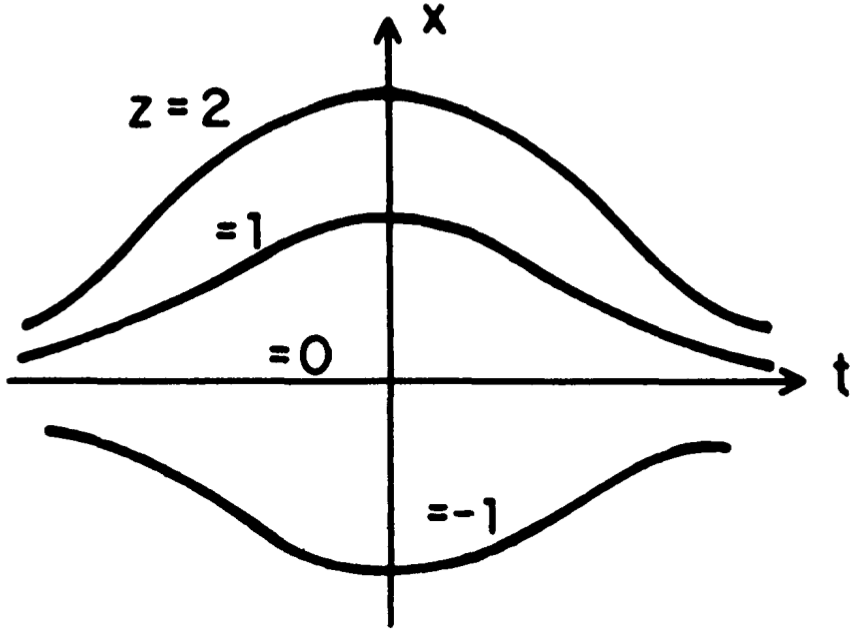
\includegraphics[width=0.5\textwidth]{instantonfig9.png}
    \caption{ \label{instantonfig9}}
  \end{figure}
\begin{tcolorbox}
    \begin{remark}
        这里稍微做一些解释. 我们把这个路径上的函数记为$x(z,t)$. 上面的条件相等于说$x(0,t)=0$以及$x(1,t)$是回弹解. 更进一步, 我们在$x(1,t)$附近展开作用量$S$:
        \[
        S(x(z,t))= S(x(1,t))+(x(z,t)-x(1,t))  \cdot \frac{\delta^{2}S}{\delta x^{2}}\biggr\vert_{x=x(1,t)}\cdot (x(z,t)-x(1,t))  
        \]
        这里的一阶导数由于经典运动方程为零, 而$(x(z,t)-x(1,t))=(z-1)\partial_{z}x(1,t)$, 我们把$\partial_{z}x(1,t)$展到$\delta^{2}S/\delta x^{2}$的本征函数, 这些本征函数只有$x_{0}$的本征值为负, 在这个方向上,
        \[
            S(x(z,t))=   S(x(1,t))-c_{0}\bigl((z-1)x_{0}\bigr)^{2}.
        \]
        因为$c_{0}$为正, 所以$S$迅速减小, 那么$\exp(-S/\hbar)$会指数增长, 因此称其为最危险的方向.
    \end{remark}    
\end{tcolorbox}
\noindent 随着$z$趋于无穷, 由于函数在转折点之后($V<0\,$)区域停留的时间越来越长, $S$趋于负无穷大; 这暗示了方程\eqref{instanton2.51}发散的很厉害.

\begin{figure}[h]
    \centering
    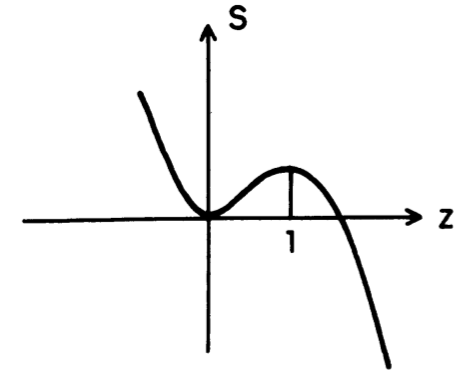
\includegraphics[width=0.5\textwidth]{instantonfig10.png}
    \caption{ \label{instantonfig10}}
  \end{figure}

如果$x=0$是$V$的绝对最小值, 这就是说, 如果$V$如图\ref{instantonfig11}(a)所示, 对于函数空间的同一路径, 情况将如图\ref{instantonfig11}(b)所示, 也就不会有方程\eqref{instanton2.48}中的发散. 现在我们解析地改变$V$使得我们从这个情况回到感兴趣的情况. 为了保持积分收敛, 我们必须把积分围道的右半端扭到复平面中. 如何改变积分围道依赖于如何将一个势变到另一个势的解析细节. 在图\ref{instantonfig12}中, 我们假定积分围道被扭到了上半平面. 使用最速下降法的标准处理, 将围道选取成: 沿着实轴从负无穷到鞍点$z=1$, 然后跑到复平面. 这个积分也就获得了虚部; 在最速下降的近似中
\begin{align}
    \operatorname{Im} J &= \operatorname{Im} \int_{1}^{1+\mi\infty} \dif z\: (2\pi\hbar)^{-1/2} \exp\Bigl(-S(1)/\hbar- \tfrac{1}{2}S''(1)(z-1)^{2}/\hbar\Bigr) \nonumber \\
    &=\tfrac{1}{2}\me^{-S(1)/\hbar} \bigl\lvert S''(1)\bigr\rvert^{-1/2} \:. \label{instanton2.52}
\end{align}
注意这个$\tfrac{1}{2}$因子; 它出现是因为积分围道只取了高斯峰的一半. (如果把积分围道扭到下半平面, 那么这个虚部就会有一个额外的符号).

\begin{figure}[h]
    \centering
    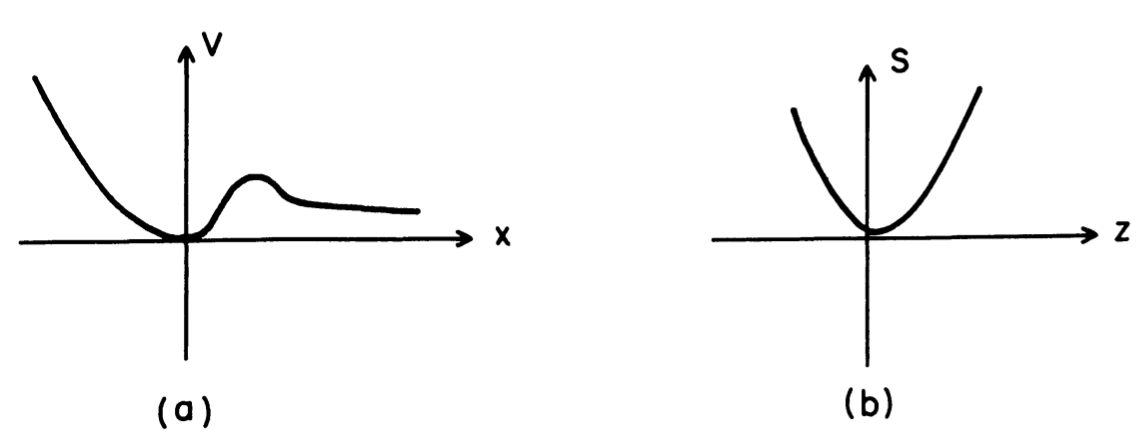
\includegraphics[width=0.9\textwidth]{instantonfig11.png}
    \caption{ \label{instantonfig11}}
  \end{figure}

  \begin{figure}[h]
    \centering
    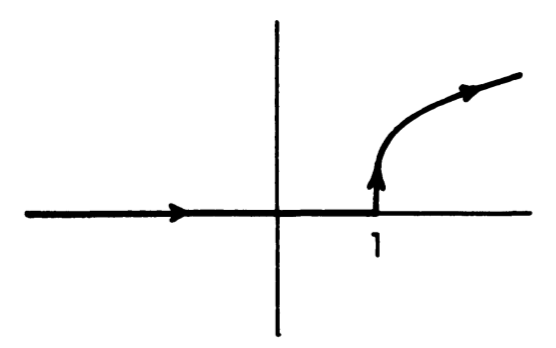
\includegraphics[width=0.5\textwidth]{instantonfig12.png}
    \caption{ \label{instantonfig12}}
  \end{figure}

我们到现在为止所研究的都是一维积分, 但由于与路径垂直的方向所联系的本征值都是非负的, 所以它们的泛函积分是平庸的. 以这种方式我们就获得了沙格列托的结果\eqref{instanton2.49}, 不同之处是对于负本征值有一个额外的$\tfrac{1}{2}$因子.


\section{规范场论中的真空结构}

\subsection{冷饭} \label{instanton:sec3.1}

这个小节主要回顾规范场论的一些基本知识, 并确定一些符号约定.

\paragraph*{李代数} 李代数的表示是$N$个反厄密矩阵$T^{a}$, $a=1,\ldots,N$, 的集合, 他们满足方程
\begin{equation}
    [T^{a},T^{b}]= c^{abc} T^{c} \:, \label{instanton3.1}
\end{equation}
其中$c$是某个紧李群$G$的结构常数. 总可以选择$T$使得$\operatorname{Tr}(T^{a}T^{b})$正比于$\delta^{ab}$, 而比例常数可能正比于表示. 嘉当内积定义成
\begin{equation}
    (T^{a},T^{b}) = \delta^{ab} \:. \label{instanton3.2}
\end{equation}
因此它正比于矩阵乘积的迹.

接下来来确定结构常数和$T$. 对于主要要处理的$SU(2)$, 选择$c^{abc}$为$\varepsilon^{abc}$. 因此, 对于同位旋表示,
\begin{equation}
    T^{a} = -\mi\sigma^{a}/2 \:, \label{instanton3.3}
\end{equation}
其中$\sigma$是泡利矩阵. 在这个情况下,
\begin{equation}
    (T^{a},T^{b})=-2\operatorname{Tr}(T^{a}T^{b}) \:. \label{instanton3.4}
\end{equation}

我们偶尔会讨论$SU(n)$, 特别是$SU(3)$. 对于它们, 结构常数和$T$的选择会使得它们对$SU(2)$子群与上面的选择相同. 因此, 对于$SU(3)$, $T^{a}$是$-\mi\lambda^{a}/2$, 其中$\lambda$是盖尔曼矩阵.

\paragraph*{规范场} 规范势是一组矢量场$A_{\mu}^{a}(x)$. 接下来定义矩阵值矢量场$A_{\mu}(x)$,
\begin{equation}
    A_{\mu}=gA_{\mu}^{a}T^{a} \:, \label{instanton3.5}
\end{equation}   
其中$g$是规范耦合常数. 场强张量$F_{\mu\nu}(x)$定义成
\begin{equation}
    F_{\mu\nu} = \partial_{\mu}A_{\nu}- \partial_{\nu}A_{\mu} + [A_{\mu},A_{\nu}] \:. \label{instanton3.6}
\end{equation}
纯规范场理论的欧几里得作用量是
\begin{equation}
    S= \frac{1}{4g^{2}} \int \dif^{4}x\: (F_{\mu\nu},F_{\mu\nu}) \:. \label{instanton3.7}
\end{equation}
有时简写成
\begin{equation}
    S=\frac{1}{4g^{2}} \int (F^{2}) \:. \label{instanton3.8}
\end{equation}

\paragraph*{规范变换} 规范变换是一个从欧几里得空间到规范群$G$的函数$g(x)$. 写成方程就是
\begin{equation}
    g(x) = \exp \bigl( \lambda^{a}(x)T^{a}\bigr) \:, \label{instanton3.9}
\end{equation}
其中$\lambda$是任意函数. (这里不要与耦合常数$g$相混淆.) 在这样一个变换下
\begin{equation}
    A_{\mu} \to g A_{\mu} g^{-1} +g \partial_{\mu} g^{-1} \:, \label{instanton3.10}
\end{equation}
以及
\begin{equation}
    F_{\mu\nu} \to g F_{\mu\nu} g^{-1} \:. \label{instanton3.11}
\end{equation}
因此$S$是规范不变的. 如果$F_{\mu\nu}$为零, 那么$A_{\mu}$是0的规范变换; 这就是说
\begin{equation}
    A_{\mu} = g\partial_{\mu}g^{-1} \:. \label{instanton3.12}
\end{equation}

\paragraph*{协变导数} 场强张量的协变导数定义成
\begin{equation}
    D_{\lambda}F_{\mu\nu} = \partial_{\lambda}F_{\mu\nu} + [A_{\lambda}, F_{\mu\nu}] \:. \label{instanton3.13}
\end{equation}
作用量\eqref{instanton3.7}给出运动方程
\begin{equation}
    D_{\mu} F_{\mu\nu} =0 \:. \label{instanton3.14}
\end{equation}
对于给定的场$\psi$, 假定它服从规范变换
\begin{equation}
    \psi \to g(x) \psi \:, \label{instanton3.15}
\end{equation}
那么$\psi$的协变导数
\begin{equation}
    D_{\mu}\psi = \partial_{\mu} \psi +A_{\mu} \psi
\end{equation}
以相同方式进行变换.

\subsection{缠绕数}

我们为什么研究作用量是有限值的规范场构型? 想当然的答案是, 作用量无限大的场构型有$\me^{-S/\hbar}=0$, 所以它们对泛函积分是不重要的. {\kaishu{这是错的}}. 实际上有限作用量的构型不重要; 更确切一些, 它们是函数空间的零测集. 我们对作用量有限的场构型感兴趣的唯一原因是我们想做半经典近似, 而如果我们把作用量无限大的场构型选做高斯积分的中心点, 那么它确实会给出零.
\begin{tcolorbox}
  \begin{remark}
    这里用有限维空间中的鞍点近似法来做一些解释说明:
    \begin{equation*}
        \int_{\mathbb{R}^{n}} g(x)\me^{\mi k f(x)} \dif x \simeq \sum_{x_{0}\in \Sigma} \me^{\mi k f(x_{0})}
        \bigl| \det (\operatorname{Hess}(f))\bigr|^{-1/2} \me^{\pi\mi \operatorname{sgn}(\operatorname{Hess}(f))/4}
        \biggl(\frac{2\pi}{k}\biggr)^{n/2}g(x_{0})
    \end{equation*}
这里的$\operatorname{Hess}(f)$是指$\partial^{2} f/\partial x_{i}\partial x_{j}$构成的海赛矩阵, 而$\operatorname{sgn}(\operatorname{Hess}(f))$是海赛矩阵的正本征值个数与负本征值个数之差, $\Sigma$则是临界点的个数.

上面所说的``有限作用量的构型是函数空间的零测集''就等同于这里的$\Sigma$是$\mathbb{R}_{n}$的零测集, 诚然在上式右边去掉这些临界点并不会对积分有影响, 但这里实际上关心的是积分关于临界点的展开, 而这样的展开仅在$k\to \infty$时才是有效的.
  \end{remark}  
\end{tcolorbox}

作用量积分的收敛性是由$A_{\mu}$在$r$很大时的行为决定的, 其中$r$是欧几里得空间中的径向变量. 为了使讨论尽可能简单, 假定$r$很大时, $A_{\mu}$可以展成$r$的负幂次的渐进级数. 因此为了使作用量有限, $F_{\mu\nu}$在$r$很大时必须比$1/r^{2}$衰减得要快; 这就是说, $F_{\mu\nu}$必须是$O(1/r^{3})$. 这暗示了$A_{\mu}$是$O(1/r^{2})$, 但这还不完全: $F_{\mu\nu}$为零只能给出$A_{\mu}$是零的规范变换. 因此$A_{\mu}$形如
\begin{equation}
    A_{\mu} = g \partial_{\mu} g^{-1} + O(1/r^{2}) \:, \label{instanton3.17}
\end{equation}
其中$g$是从4维空间到群$G$的$O(1)$函数, 这就是说, 它是角变量的函数.

\begin{remark}
这里的$g(x)$是紧群$G$上的元素, 所以它最多是$O(1)$的, 我们这里只关心$A_{\mu}$在$r\to\infty$时行为, 所以$g$只需要是角变量的函数.    
\end{remark}

因此, 每个作用量有限的场构型都会联系到角变量的一个群元值函数, 也就是说, 一个三维超球面$S^{3}$到规范群$G$的映射. 当然, 这个分配不是规范不变的. 在规范变换$h(x)$下,
\begin{equation}
    A_{\mu } \to h A_{\mu}h^{-1} + h \partial_{\mu}h^{-1} \:. \label{instanton3.18}
\end{equation}
因此,
\begin{equation}
    g\to hg + O(1/r^{2}) \:. \label{instanton3.19}
\end{equation}
\begin{tcolorbox}
    把方程\eqref{instanton3.17}代入\eqref{instanton3.18}右边, 得到
    \begin{align*}
        A_{\mu} &\to hg(\partial_{\mu}g^{-1})h^{-1} +h\partial_{\mu}h^{-1} \\
        &= hg \Bigl( (\partial_{\mu}g^{-1})h^{-1} +g^{-1}\partial_{\mu}h^{-1}\Bigr) =hg \partial_{\mu} (g^{-1}h^{-1}) \:. 
    \end{align*}
    即方程\eqref{instanton3.19}
\end{tcolorbox}

如果我们能选择$h$使得它在无穷远处等于$g^{-1}$, 我们可以把$g$变换到1然后从方程\eqref{instanton3.17}中消掉它. 然而, 这一般是不可能的. 
原因是$h$不仅要是无穷远处的超球面上的连续函数, 也得在整个四维空间连续, 也就是说, 沿着$r$把整个四维空间划成逐层嵌套的超球面, 在这些连续变换的超球面上, $h$是连续的. 特别地, $h$在原点必须是一个常数. 因此, 无穷远处的$h$不可能是$S^{3}$上的一般函数, 而是可以通过连续形变可以从常函数得到的连续函数. 由于任何常数规范变换都可以从恒等变换做连续形变得到(所有规范群都是连通的), 我们也可以说无穷远处的$h$可以通过对$h=1$做连续形变得到.

给定从一个拓扑空间到另一个拓扑空间的两个映射, 如果一个映射可以连续形变到另一个, 数学家称这两个函数是“同伦的”或者“处在同一个同伦类中”. 我们刚才证明了我们可以通过规范变换把$g(x)$变换到任何与$g(x)$同伦的映射, 但我们无法把它变换到另一个同伦类中的函数. 因此, 与有限作用量场构型相联系的不是$S^{3}$到$G$的映射, 而是这种映射的同伦类. 我们的任务是对物理上感兴趣的$G$找到这些同伦类.

我们先来做个热身练习, 考虑一个几何可视化的简化版. 我们将处理最简单的规范群, $U(1)$. 这样规范场论就是普通的电磁理论. (然而, 我们这里所采用的符号约定是\ref{instanton:sec3.1}节中确定的那些, 因此$A_{\mu}$将是纯虚的.) 另外, 我们将考虑二维空间而不是四维空间. 我们仍然要研究满足方程\eqref{instanton3.17}的场, 尽管这个条件不再是作用量有限的结果. 由于我们处理的是二维空间, 所以取代前面的超球面$S^{3}$, 我们这里面对的是一个圆$S^{1}$.

现在开始处理:
\begin{enumerate}
    \item $G$是复平面中的单位圆; 因此, 从拓扑上将, $G$也是$S^{1}$, 所以我们必须研究从$S^{1}$到$S^{1}$的映射的同伦类. 我们将按照传统方式用在$0$到$2\pi$之间取值的$\theta$来标记空间中的圆, 即映射的定义域.
    \item 定义一些从$S^{1}$到$S^{1}$的标准映射. 一个是平庸映射,
    \begin{subequations} \label{instanton3.20}
        \begin{gather}
            g^{(0)}(\theta)=1 \:. \label{instanton3.20a} \\
        \intertext{另一个是单位映射,}
            g^{(1)}(\theta) = \me^{\mi\theta} \:. \label{instanton3.20b}\\
        \intertext{它们都是如下映射族}
            g^{(\nu)}(\theta) = [g^{(1)}(\theta)]^{\nu} = \me^{\mi\nu\theta}  \tag{3.20c} \label{instanton3.20c} 
        \end{gather}  
    \end{subequations}
    的成员, 其中$\nu$是整数. $\nu$被称为``缠绕数''.
    \item 每个从$S^{1}$到$S^{1}$的映射同伦于映射\eqref{instanton3.20c}中的一个. 这是著名的事实$\pi_{1}(S^{1})=\mathbb{Z}$. 即圆的第一同伦群是整数加法群.
    \item 上述缠绕数可以有如下积分公式给出:
    \begin{equation}
        \nu = \frac{\mi}{2\pi} \int_{0}^{2\pi} \dif\theta\: g\frac{\dif }{\dif\theta} g^{-1}\:. \label{instanton3.21}
    \end{equation}
    对于标准映射\eqref{instanton3.20c}, 这显然是成立的. 这个量在连续变换下也是不变的. 这点可以通过考虑无限小形变来证明. 一个无限小的形变可以写成
    \begin{equation}
        \delta g =\mi (\delta\lambda) g\:, \label{instanton3.22}
    \end{equation}
    其中$\delta\lambda$是圆上的无限小实函数. 因此
    \begin{align}
        \delta\biggl(g\frac{\dif}{\dif\theta} g^{-1}\biggr) &= (\delta g)\frac{\dif}{\dif\theta} g^{-1}+
        g\frac{\dif}{\dif\theta} (\delta g^{-1})=\mi\delta \lambda \,g \frac{\dif}{\dif\theta} g^{-1} 
        -\mi g \frac{\dif}{\dif\theta} (\delta\lambda\,g^{-1}) \nonumber \\
        &=-\mi \frac{\dif}{\dif\theta} \delta\lambda \label{instanton3.23}
    \end{align}
    这里使用了$\delta g^{-1}= -g^{-1}(\delta g) g^{-1}$, 由此看出这不会对$\nu$产生影响.
    \item 如果
    \begin{subequations}
        \begin{gather}
        g(\theta) = g_{1}(\theta)g_{2}(\theta) \:, \tag{3.24a} \label{instanton3.24a} \\
    \intertext{那么}
        \nu= \nu_{1}+\nu_{2} \:. \tag{3.24b} \label{instanton3.24b}
        \end{gather}
    \end{subequations}
    证明是简单的: 对$g_{1}$做形变使得它在上半圆为1, 对$g_{2}$做形变使得它在下半圆为1.
    \item 我们定义
    \begin{equation}
        G_{\mu} =\frac{\mi}{2\pi} \varepsilon_{\mu\nu} A_{\nu} \:. \label{instanton3.25}
    \end{equation}
    通过方程\eqref{instanton3.17}和\eqref{instanton3.21},
    \begin{equation}
        \nu = \lim_{r\to\infty} \int_{0}^{2\pi} r \dif \theta\: \hat{r}_{\mu}G_{\mu} \:, \label{instanton3.26}
    \end{equation}
    其中$\hat{r}_{\mu}$是径向单位矢量. 因此通过高斯定理,
    \begin{equation}
        \nu = \int\dif^{2}x\: \partial_{\mu}G_{\mu} \:. \label{instanton3.27}
    \end{equation}
    这样,
    \begin{equation}
        \nu = \frac{\mi}{4\pi}\int\dif^{2}x\: \varepsilon_{\mu\nu}F_{\mu\nu} \:. \label{instanton3.27}
    \end{equation}
    \begin{remark}
        这里使用了$\hat{r}_{\mu}\varepsilon_{\mu\nu}A_{\nu}=\cos\theta A_{y}-\sin\theta A_{x}= r^{-1} g\partial_{\theta} g^{-1}$
    \end{remark}
\end{enumerate}

\subsection{多个真空}

\subsection{瞬子: 一般情形}

\subsection{瞬子: 特殊情形}

\section{$1+1$维中的阿贝尔Higgs模型}



\section{$U(1)$问题的't Hooft解决方案}

\subsection{介子失踪之谜}

\subsection{准备工作: 欧几里得费米场}

\subsection{准备工作: 手征沃德恒等式}

\subsection{QCD(幼儿版)}


\subsection{QCD(真实版)}

\subsection{杂录}


\section{假时空的命运}

\subsection{不稳定真空}

\subsection{回弹}

\subsection{薄壁近似}

\subsection{假真空的命运}

\subsection{行列式与重整化}

\subsection{待解答的问题}


\part{超弦理论以及拓展}


\setcounter{section}{0}%更改chapter的计数器值
%\numberwithin{equation}{chapter}%公式计数器从属于节计数器
\numberwithin{equation}{section}%公式计数器从属于节计数器
\numberwithin{figure}{section}%图计数器从属于节计数器
\setcounter{chapter}{9}

\chapter{I型超弦和II型超弦}


\section{超共形代数}

玻色弦中, 质壳条件
\begin{equation}
    p_{\mu}p^{\mu}+m^{2}=0 \label{10.1.1}
\end{equation}
来自于物理态条件
\begin{equation}
    L_{0}\lvert \psi\rangle = 0\: , \label{10.1.2}
\end{equation}
在闭弦中还得加上$\,\tilde{L}_{0}\lvert\psi\rangle=0\,$. 为了得到费米子, 我们需要\,Dirac\,方程
\begin{equation}
    \mi p_{\mu} \Gamma^{\mu}+m=0\:. \label{10.1.3}
\end{equation}

在玻色弦中, $L_{0}\,$和$\,\tilde{L}_{0}\,$是能动量张量$(T_{B},\tilde{T}_{B})$的质心模. 现在我们要引入新的守恒量$\,T_{F}\,$和$\,\tilde{T}_{F}\,$, 使得它们的质心模给出\,Dirac\,方程. 注意到, 时空动量$\,p^{\mu}\,$是世界面流$(\partial X^{\mu},\bar{\partial}X^{\mu} )$的质心模, 我们现在期待代数满足
\begin{equation}
    \{\Gamma^{\mu},\Gamma^{\nu}\}=2\eta^{\mu\nu} \:, \label{10.1.4}
\end{equation}
的\,$\Gamma$\,矩阵是反对易世界面场$\,\psi^{\mu}\,$的质心模.

现在来考察世界面作用量
\begin{equation}
    S=\frac{1}{4\uppi}\int\dif^{2}z \:
    \left(
    \frac{2}{\alpha^{\prime}}\partial X^{\mu}\bar{\partial}X_{\mu} +\psi^{\mu}\bar{\partial}\psi_{\mu}
    +\tilde{\psi}^{\mu}\partial\tilde{\psi}_{\mu}
    \right)\:.\label{10.1.5}
\end{equation}
$XX\,$的OPE是
\begin{equation}
    X^{\mu}(z,\bar{z})X^{\nu}(0,0)\sim -\frac{\alpha^{\prime}}{2}\eta^{\mu\nu}\ln\lvert z\rvert^{2}\:.\label{10.1.6}
\end{equation}
$\psi\,$和$\,\tilde{\psi}\,$分别是全纯和反全纯的, 它们的\,OPE\,是
\begin{equation}
    \psi^{\mu}(z)\psi^{\nu}(0)\sim\frac{\eta^{\mu\nu}}{z}\:,\qquad
     \tilde{\psi}^{\mu}(\bar{z})\tilde{\psi}^{\nu}(0)\sim\frac{\eta^{\mu\nu}}{\bar{z}}\: \label{10.1.7}
\end{equation}
{\emph{世界面超流}}是
\begin{equation}
    T_{F}(z)=\mi(2/\alpha^{\prime})^{1/2}\psi^{\mu}(z)\partial X_{\mu}(z)\:,\qquad
     \tilde{T}_{F}(\bar{z})=\mi(2/\alpha^{\prime})^{1/2}\tilde{\psi}^{\mu}(\bar{z})\bar{\partial} X_{\mu}(\bar{z})
     \:.\label{10.1.8}
\end{equation}

这给出希望的结果: $\psi_{0}^{\mu}\,$和$\,\tilde{\psi}_{0}^{\mu}\,$模将满足\,Gamma\,矩阵代数, 而$\,T_{F}\,$和$\,\tilde{T}_{F}\,$的质心模有\,Dirac\,算符的形式. 

从\,OPE\,和\,Ward\,恒等式可以得出: 流
\begin{equation}
    j^{\eta}(z)=\eta(z)T_{F}(z)\:, \qquad
    \tilde{\jmath}(\bar{z})=\bar{\eta}(\bar{z}) \tilde{T}_{F}(\bar{z}) \label{10.1.9}
\end{equation}
生成了{\emph{超共形变换}}
\begin{subequations}
\begin{align}
     \epsilon^{-1}(2/\alpha^{\prime})^{1/2}\delta X^{\mu}(z,\bar{z}) &= \eta(z)\psi^{\mu}(z) + \eta(z)^{\ast} \tilde{\psi}^{\mu}(\bar{z})\:, \label{10.1.10a} \\
      \epsilon^{-1}(2/\alpha^{\prime})^{1/2}\delta \psi^{\mu}(z) &= -\eta(z)\partial X^{\mu}(z) \:, \label{10.1.10b}  \\
      \epsilon^{-1}(2/\alpha^{\prime})^{1/2}\delta\tilde{\psi}^{\mu}(\bar{z}) &=-\eta(z)^{\ast}\bar{\partial} X^{\mu}(\bar{z}) \:. \label{10.1.10c}
\end{align}
\end{subequations}
这个变换将对易场$\,X^{\mu}\,$和反对易场$\,\psi^{\mu}\,$和$\,\tilde{\psi}^{\mu}\,$混在了一起, 所以$\,\eta(z)\,$必须是反对易参量. 

\begin{tcolorbox}
\noindent 我们现在来考察$\,T_{F},\tilde{T}_{F}\,$%
与\,$X,\psi ,\tilde{\psi}\,$的\,OPE\,: \\
(1)
\begin{align*}
T_{F}(w)X^{\mu }(z,\bar{z}) &=\mi(2/\alpha ^{\prime })^{1/2}\psi ^{\nu
}(w)\partial X_{\nu }(w)X^{\mu }(z,\bar{z}) \\
&=\mi(2/\alpha ^{\prime })^{1/2}\psi ^{\nu }(w)\partial _{w}\delta _{\nu
}^{\mu }\left( -\frac{\alpha ^{\prime }}{2}\ln \lvert z-w\rvert
^{2}\right)  \\
&=-\mi\left( \alpha ^{\prime }/2\right) ^{1/2}\frac{\psi ^{\mu }(w)}{w-z}
\end{align*}%
类似地可以得到\[
\tilde{T}_{F}(\bar{w})X^{\mu }(z,\bar{z})=-\mi\left( \alpha ^{\prime
}/2\right) ^{1/2}\frac{\tilde{\psi}^{\mu }(\bar{w})}{\bar{w}-\bar{z}}
\]%
利用Ward恒等式\[
\frac{1}{\mi\epsilon }\delta \mathscr{A}(z,\bar{z})=\operatorname{Res}_{w\rightarrow z}j(w)\mathscr{A}(z,%
\bar{z})+\overline{\operatorname{Res}}_{\bar{w}\rightarrow \bar{z}}\tilde{\jmath}(\bar{w})\mathscr{A}(z,\bar{z}%
)
\]%
得到\begin{align*}
\frac{1}{\mi\epsilon }\delta X(z,\bar{z}) &=\eta (z)\left( -\mi\left( \alpha
^{\prime }/2\right) ^{1/2}\psi ^{\mu }(z)\right) +\eta (z)^{\ast }\left(
-\mi\left( \alpha ^{\prime }/2\right) ^{1/2}\tilde{\psi}^{\mu }(\bar{z}%
)\right)  \\
\epsilon ^{-1}\left( 2/\alpha ^{\prime }\right) ^{1/2}\delta X(z,\bar{z})
&=\eta (z)\psi ^{\mu }(z)+\eta (z)^{\ast }\tilde{\psi}^{\mu }(\bar{z})
\end{align*}%
(2)%
\begin{align*}
T_{F}(w)\psi ^{\mu }(z) &=\mi(2/\alpha ^{\prime })^{1/2}\psi ^{\nu
}(w)\partial X_{\nu }(w)\psi ^{\mu }(z) \\
&=\mi(2/\alpha ^{\prime })^{1/2}\frac{\eta ^{\mu \nu }}{w-z}\partial X_{\nu
}(w) \\
&=\mi(2/\alpha ^{\prime })^{1/2}\frac{\partial X^{\mu }(w)}{w-z}
\end{align*}%
利用Ward恒等式得到\begin{align*}
\frac{1}{i\epsilon }\delta \psi ^{\mu }(z) &=\eta (z)\left( \mi(2/\alpha
^{\prime })^{1/2}\partial X^{\mu }(z)\right)  \\
\epsilon ^{-1}(\alpha ^{\prime }/2)^{1/2}\delta \psi ^{\mu }(z) &=-\eta
(z)\partial X^{\mu }(z)
\end{align*}%
(3) 类似地, 就得到(\ref{10.1.10c})
\end{tcolorbox}

两个超共形变换的对易子是共形变换,
\begin{equation}
    \delta_{\eta_{1}}\delta_{\eta_{2}}-\delta_{\eta_{2}}\delta_{\eta_{1}}=\delta_{v}\:,\qquad
    v(z)= -2\eta_{1}(z)\eta_{2}(z) \:, \label{10.1.11}
\end{equation}
类似地, 共形变换和超共形变换的对易子是超共形变换.
\begin{tcolorbox}
首先对$\,X\,$验证(\ref{10.1.11}), 可知
\begin{align*}
    \delta_{\eta_{1}}\delta_{\eta_{2}}X &=  (\alpha^{\prime}/2)^{1/2}
    \delta_{\eta_{1}}(\eta_{2}(z)\psi^{\mu}(z) + \eta_{2}(z)^{\ast} \tilde{\psi}^{\mu}(\bar{z})) \\
    &=-(\alpha^{\prime}/2)^{1/2} (2/\alpha^{\prime})^{1/2}
    (\eta_{2}(z)\eta_{1}(z)\partial X^{\mu}(z) + \eta_{2}(z)^{\ast} \eta_{1}(z)^{\ast}\bar{\partial}X^{\mu}(\bar{z}))  \\
    &=
    \eta_{1}(z)\eta_{2}(z)\partial X^{\mu}(z) +
    \eta_{1}(z)^{\ast} \eta_{2}(z)^{\ast}\bar{\partial}X^{\mu}(\bar{z})
\end{align*}
所以
\begin{equation*}
    [\delta_{\eta_{1}},\delta_{\eta_{2}}]X= 
     2\eta_{1}\eta_{2}\partial X^{\mu} + 2\eta_{1}^{\ast} \eta_{2}^{\ast}\bar{\partial}X^{\mu}
     =\delta_{v}X
\end{equation*}
参看(\textcolor{red}{2.4.7}).

接下来对$\,\psi\,$验证(\ref{10.1.11}),
可知\begin{align*}
\delta _{\eta _{1}}\delta _{\eta _{2}}\psi ^{\mu } &=-\delta _{\eta
_{1}}\left( \eta _{2}(z)\partial X^{\mu }(z)\right) =-\eta _{2}(z)\partial
(\delta _{\eta _{1}}X^{\mu }(z)) \\
&=-\eta _{2}(z)\partial (\eta _{1}(z)\psi ^{\mu }(z)+\eta _{1}(z)^{\ast }%
\tilde{\psi}^{\mu }(\bar{z})) \\
&=-\eta _{2}\eta _{1}\partial \psi ^{\mu }-\eta _{2}(\partial \eta
_{1})\psi ^{\mu }
\end{align*}%
所以\begin{align*}
\lbrack \delta _{\eta _{1}},\delta _{\eta _{2}}]\psi ^{\mu } &=-\eta
_{2}\eta _{1}\partial \psi ^{\mu }-\eta _{2}(\partial \eta _{1})\psi ^{\mu
}+\eta _{1}\eta _{2}\partial \psi ^{\mu }+\eta _{1}(\partial \eta _{2})\psi
^{\mu } \\
&=2\eta _{1}\eta _{2}\partial \psi ^{\mu }+\partial (\eta _{1}\eta
_{2})\psi ^{\mu }
\end{align*}%
由于$\psi $是$(\frac{1}{2},0)$场, 这正是$\delta _{v}\psi $, 实际是对于权重为$(h,0)$的primary场$\mathcal{O}$, 根据(2.4.16)%
\[
T(z)\mathcal{O}(w,\bar{w})=\frac{h}{(z-w)^{2}}\mathcal{O}(w,\bar{w})+\frac{1}{(z-w)}\partial \mathcal{O}(w,%
\bar{w})+\cdots \text{ ,}
\]%
那么Ward恒等式给出\begin{align*}
\frac{1}{\mi }\delta _{v}\mathcal{O} &=\operatorname{Res}_{z\to w}\Bigl(\mi v(z)T(z)\mathcal{O}(w,%
\bar{w})\Bigr) \\
\delta _{v}\mathcal{O} &=-\left( h(\partial v)\mathcal{O}+v\partial \mathcal{O}\right)
\end{align*}
对于$\,\tilde{\psi}\,$类似.

现在来考察共形变换和超共形变换的对易子, 首先是$X$%
\begin{align*}
\delta _{\eta }\delta _{v}X &=\delta _{\eta }(-v\partial X-v^{\ast }\bar{%
\partial}X)=-v\partial \left( \delta _{\eta }X\right) -v^{\ast }\bar{\partial%
}\left( \delta _{\eta }X\right)  \\
&=-v\partial \left( \eta \psi +\eta ^{\ast }\tilde{\psi}\right) -v^{\ast }%
\bar{\partial}\left( \eta \psi +\eta ^{\ast }\tilde{\psi}\right)  \\
&=-v(\partial \eta )\psi -v\eta \partial \psi -v^{\ast }(\partial \eta
)^{\ast }\tilde{\psi}-v^{\ast }\eta ^{\ast }\bar{\partial}\tilde{\psi}
\end{align*}%
而
\begin{align*}
\delta _{v}\delta _{\eta }X &=\delta _{v}(\eta \psi +\eta ^{\ast }\tilde{%
\psi})=\eta \left( -v\partial \psi -\tfrac{1}{2}\left( \partial v\right) \psi
\right) +\eta ^{\ast }\left( -v^{\ast }\bar{\partial}\tilde{\psi}-\tfrac{1}{2}%
\left( \partial v\right) ^{\ast }\tilde{\psi}\right)
\end{align*}%
\end{tcolorbox}
\begin{tcolorbox}
所以\begin{align*}
\lbrack \delta _{\eta },\delta _{v}]X &=-v(\partial \eta )\psi -v\eta
\partial \psi -v^{\ast }(\partial \eta )^{\ast }\tilde{\psi}-v^{\ast }\eta
^{\ast }\bar{\partial}\tilde{\psi} \\
&\quad+\eta v\partial \psi +\tfrac{1}{2}\eta \left( \partial v\right) \psi +\eta
^{\ast }v^{\ast }\bar{\partial}\tilde{\psi}+\tfrac{1}{2}\eta ^{\ast }\left(
\partial v\right) ^{\ast }\tilde{\psi} \\
&=-v(\partial \eta )\psi -v^{\ast }(\partial \eta )^{\ast }\tilde{\psi}+%
\tfrac{1}{2}\eta \left( \partial v\right) \psi +\tfrac{1}{2}\eta ^{\ast
}\left( \partial v\right) ^{\ast }\tilde{\psi} \\
&=\delta _{\eta ^{\prime }}X
\end{align*}%
其中\[
\eta ^{\prime }=-v\partial \eta +\tfrac{1}{2}\eta \partial v
\]%
对于$\psi $%
\begin{align*}
\delta _{\eta }\delta _{v}\psi  &=\delta _{\eta }\left( -v\partial \psi +%
\tfrac{1}{2}(\partial v)\psi \right) =-v\partial \left( \delta _{\eta }\psi
\right) +\tfrac{1}{2}(\partial v)\delta _{\eta }\psi  \\
&=-v\partial \left( \eta \partial X\right) -\frac{1}{2}(\partial v)\eta
\partial X \\
&=-v\eta \partial ^{2}X-v\partial \eta \partial X-\tfrac{1}{2}(\partial
v)\eta \partial X
\end{align*}%
而\begin{align*}
\delta _{v}\delta _{\eta }\psi  &=\delta _{v}(\eta \partial X)=\eta
\partial (\delta _{v}X)=\eta \partial (-v\partial X-v^{\ast }\bar{\partial}X)
\\
&=-\eta \partial v\partial X-\eta v\partial ^{2}X
\end{align*}%
所以\begin{align*}
\lbrack \delta _{\eta },\delta _{v}]\psi  &=-v\eta \partial ^{2}X-v\partial
\eta \partial X-\tfrac{1}{2}(\partial v)\eta \partial X+\eta \partial
v\partial X+\eta v\partial ^{2}X \\
&=-v\partial \eta \partial X+\tfrac{1}{2}(\partial v)\eta \partial X \\
&=\delta _{\eta ^{\prime }}X
\end{align*}%
对于$\tilde{\psi}$类似.
\end{tcolorbox}
从上面我们看到共形变换加上超共形变换封闭, 它们合起来构成了{\emph{超共形代数}}. 以流的形式, 这意味着$T_{F}$与$T_{B}$的OPE封闭, 不过这时的$T_{B}$要加入费米子部分
\begin{equation}
    T_{B}=-\frac{1}{\alpha^{\prime}}\partial X^{\mu}\partial X_{\mu}-\frac{1}{2}\psi^{\mu}\partial\psi_{\mu}
\end{equation}
它们的OPE是
\begin{subequations}
\begin{align}
    T_{B}(z)T_{B}(0)&\sim \frac{3D}{4z^{4}}+\frac{2}{z^{2}}T_{B}(0)+\frac{1}{z}\partial T_{B}(0)\:,\label{10.1.13a}\\
    T_{B}(z)T_{F}(0)&\sim \frac{3}{2z^{2}}T_{F}(0)+\frac{1}{z}\partial T_{F}(0)\:,\label{10.1.13b}\\
    T_{F}(z)T_{F}(0)&\sim \frac{D}{z^{3}}+\frac{2}{z}T_{B}(0) \:,\label{10.1.13c}
\end{align}
\end{subequations}
反全纯流有类似的结果. $T_{B}T_{F}$的OPE暗示了$T_{F}$是权重为$(\frac{3}{2},0)$的张量. 每个标量为中性荷贡献1, 而每个旋量为中心荷贡献$\frac{1}{2}$, 所以总的中心荷是
\begin{equation}
    c=(1+\tfrac{1}{2})D=\tfrac{3}{2}D\:.\label{10.1.14}
\end{equation}
同玻色弦一样, $T_{B}$和$T_{F}$是态上的约束代数, 它们会从频谱中移去一些态.

更一般的$N=1$超共形代数是
\begin{subequations}
\begin{align}
    T_{B}(z)T_{B}(0)&\sim \frac{c}{2z^{4}}+\frac{2}{z^{2}}T_{B}(0)+\frac{1}{z}\partial T_{B}(0)\:,\label{10.1.15a}\\
    T_{B}(z)T_{F}(0)&\sim \frac{3}{2z^{2}}T_{F}(0)+\frac{1}{z}\partial T_{F}(0)\:,\label{10.1.15b}\\
    T_{F}(z)T_{F}(0)&\sim \frac{2c}{3z^{3}}+\frac{2}{z}T_{B}(0) \:,\label{10.1.15c}
\end{align}
\end{subequations}

\begin{tcolorbox}
对于$T_{B}$, 我们可以将其写成$T_{B}^{X}$与$T_{B}^{\psi }$的和, 关于$T_{B}^{X}$的部分已经在2.2%
节讨论过, 参看(2.2.11)和(2.4.22),
现在只需考察$T_{B}^{\psi }$.%
\begin{align*}
T_{B}^{\psi }(z)T_{B}^{\psi }(\omega ) &=\frac{1}{4}:\psi ^{\mu
}(z)\partial _{z}\psi _{\mu }(z)::\psi ^{\nu }(w)\partial _{w}\psi _{\nu
}(w): \\
&=-\frac{1}{4}\frac{\eta ^{\mu \nu }}{z-w}\partial _{z}\partial _{w}\frac{%
\eta _{\mu \nu }}{z-w}+\frac{1}{4}\partial _{w}\frac{\delta _{\nu }^{\mu }}{%
z-w}\partial _{z}\frac{\delta _{\nu }^{\mu }}{z-w} \\
&\quad+\frac{1}{4}\partial _{w}\frac{\delta _{\nu }^{\mu }}{z-w}\partial
_{z}\psi _{\mu }(z)\psi ^{\nu }(w)-\frac{1}{4}\frac{\eta ^{\mu \nu }}{z-w}%
\partial _{z}\psi _{\mu }(z)\partial _{w}\psi _{\nu }(w) \\
&\quad+\frac{1}{4}\partial _{z}\frac{\delta _{\mu }^{\nu }}{z-w}\psi ^{\mu
}(z)\partial _{w}\psi _{v}(w)-\frac{1}{4}\partial _{z}\partial _{w}\frac{%
\eta _{\mu \nu }}{z-w}\psi ^{\mu }(z)\psi ^{\nu }(w) \\
&=\frac{1}{4}\frac{2D}{(z-w)^{4}}+\frac{1}{4}\frac{-D}{(z-w)^{4}}+\frac{1}{4%
}\frac{1}{\left( z-w\right) ^{2}}\partial _{z}\psi ^{\mu }(z)\psi _{\mu }(w)
\\
&\quad-\frac{1}{4}\frac{1}{(z-w)^{2}}\psi ^{\mu }(z)\partial _{w}\psi _{\mu }(w)-%
\frac{1}{4}\frac{1}{z-w}\partial _{z}\psi ^{\mu }(z)\partial _{w}\psi _{\mu
}(w) \\
&\quad-\frac{1}{4}\frac{-2}{(z-w)^{3}}\psi ^{\mu }(z)\psi _{\mu }(w) \\
&=\frac{D}{4(z-w)^{4}}+\frac{1}{4}\frac{1}{\left( z-w\right) ^{2}}\partial
_{w}\psi ^{\mu }(w)\psi _{\mu }(w)+\frac{1}{4}\frac{1}{z-w}\partial
_{w}^{2}\psi ^{\mu }(w)\psi _{\mu }(w) \\
&\quad-\frac{1}{4}\frac{1}{(z-w)^{2}}\psi ^{\mu }(w)\partial _{w}\psi _{\mu }(w)-%
\frac{1}{2}\frac{1}{(z-w)}\partial _{w}\psi ^{\mu }(w)\partial _{w}\psi
_{\mu }(w) \\
&\quad+\frac{1}{2}\frac{1}{(z-w)^{2}}\partial _{w}\psi ^{\mu }\psi _{\mu
} +\frac{1}{4(z-w)}\partial _{w}^{2}\psi ^{\mu }\psi _{\mu } \\
&=\frac{D}{4(z-w)^{4}}-\frac{1}{(z-w)^{2}}\psi _{\mu }\partial _{w}\psi
^{\mu }-\frac{1}{2}\frac{1}{(z-w)}\left( \psi _{\mu }\partial _{w}^{2}\psi
^{\mu }+\partial _{w}\psi ^{\mu }\partial _{w}\psi _{\mu }\right)  \\
&=\frac{D}{4(z-w)^{4}}+\frac{2T_{B}^{\psi }(w)}{(z-w)^{2}}+\frac{\partial
T_{B}^{\psi }(w)}{z-w}
\end{align*}
需要注意的是, 第一个等号后出现负号是因为$\,\psi\,$的反对易性, 同样由于反对易性, 所以$\,(z-w)^{-3}\psi^{\mu}(w)\psi_{\mu}(w)\,$为零, 加上$T_{B}^{X}(x)T_{B}^{X}(w)$的OPE, 我们就给出了(\ref{10.1.13a}).
\end{tcolorbox}

\begin{tcolorbox}
接下来证明(\ref{10.1.13b})%
\begin{align*}
T_{B}(z)T_{F}(\omega ) &=\left( -\frac{1}{\alpha ^{\prime }}\partial
_{z}X^{\mu }\partial _{z}X_{\mu }-\frac{1}{2}\psi ^{\mu }\partial _{z}\psi
_{\mu }\right) \left( \mi\sqrt{\frac{2}{\alpha ^{\prime }}}\psi ^{\nu
}(w)\partial _{w}X_{\nu }(w)\right)  \\
&=-\mi\sqrt{\frac{2}{\alpha ^{\prime 3}}}2\partial _{z}\partial _{w}\frac{%
-\alpha ^{\prime }}{2}\ln |z-w|^{2}\partial _{z}X_{\mu }\psi ^{\mu }(w) \\
&\quad+\frac{\mi}{2}\sqrt{\frac{2}{\alpha ^{\prime }}}\frac{\eta ^{\mu \nu }}{z-w}%
\partial _{z}\psi _{\mu }\partial _{w}X_{\nu }(w)-\frac{\mi}{2}\sqrt{\frac{2}{%
\alpha ^{\prime }}}\partial _{z}\frac{\delta _{\mu }^{\nu }}{z-w}\psi ^{\mu
}(z)\partial _{w}X_{\nu }(w) \\
&=\mi\sqrt{\frac{2}{\alpha ^{\prime }}}\frac{1}{(z-w)^{2}}\partial _{z}X_{\mu
}\psi ^{\mu }(w)+\frac{\mi}{2}\sqrt{\frac{2}{\alpha ^{\prime }}}\frac{1}{z-w}%
\partial _{z}\psi _{\mu }\partial _{w}X^{\mu }(w) \\
&\quad+\frac{\mi}{2}\sqrt{\frac{2}{\alpha ^{\prime }}}\frac{1}{(z-w)^{2}}\psi
^{\nu }(z)\partial _{w}X_{\mu }(w) \\
&=\frac{3}{2}\mi\sqrt{\frac{2}{\alpha ^{\prime }}}\frac{1}{(z-w)^{2}}\psi
^{\mu }\partial _{w}X_{\mu }(w)+\mi\sqrt{\frac{2}{\alpha ^{\prime }}}\frac{1}{%
z-w}\psi ^{\mu }\partial _{w}^{2}X_{\mu }(w) \\
&\quad\frac{\mi}{2}\sqrt{\frac{2}{\alpha ^{\prime }}}\frac{1}{z-w}\partial
_{w}\psi _{\mu }\partial _{w}X^{\mu }(w)+\frac{\mi}{2}\sqrt{\frac{2}{\alpha
^{\prime }}}\frac{1}{z-w}\partial _{w}\psi ^{\nu }(w)\partial _{w}X_{\mu }(w)\\
&=\frac{3}{2(z-w)^{2}}T_{F}(w)+\frac{\mi}{z-w}\sqrt{\frac{2}{\alpha ^{\prime }%
}}\left( \psi ^{\mu }\partial _{w}^{2}X_{\mu }(w)+\partial _{w}\psi _{\mu
}\partial _{w}X^{\mu }(w)\right)  \\
&=\frac{3}{2(z-w)^{2}}T_{F}(w)+\frac{1}{z-w}\partial T_{F}(w)\text{ ,}
\end{align*}
最后我们来考察$T_{F}(z)T_{F}(w)$
\begin{align*}
T_{F}(z)T_{F}(w) &=-(2/\alpha ^{\prime })\psi ^{\mu }(z)\partial X_{\mu
}(z)\psi ^{\nu }(w)\partial X_{\nu }(w) \\
&=-(2/\alpha ^{\prime })\frac{\eta ^{\mu \nu }}{z-w}\partial _{z}\partial
_{w}[(-\alpha ^{\prime }/2)\eta _{\mu \nu }\ln |z-w|^{2}] 
-(2/\alpha ^{\prime })\frac{\eta ^{\mu \nu }}{z-w}\partial X_{\mu
}(z)\partial X_{\nu }(w)\\
&\quad-(2/\alpha ^{\prime })\psi ^{\mu }(z)\psi ^{\nu
}(w)\partial _{z}\partial _{w}[(-\alpha ^{\prime }/2)\eta _{\mu \nu }\ln
|z-w|^{2}] \\
&=\frac{D}{(z-w)^{3}}+\frac{2}{z}T_{B}^{X}(w)+\psi ^{\mu }(z)\psi _{\mu }(w)%
\frac{1}{(z-w)^{2}} \\
&=\frac{D}{(z-w)^{3}}+\frac{2}{z}T_{B}^{X}(w)-\psi _{\mu }(w)\partial
_{w}\psi ^{\mu }(w)\frac{1}{z-w} \\
&=\frac{D}{(z-w)^{3}}+\frac{2}{z}T_{B}(w)
\end{align*}
这就证明了(\ref{10.1.13c})
\end{tcolorbox}

\subsection*{Free SCFT}
反对易$bc$理论加上对易$\beta\gamma$系统会构成自由的SCFT. 二者的权重分别是
\begin{subequations}
\begin{align}
    h_{b}&=\lambda\:,\qquad h_{c}=1-\lambda \:, \label{10.1.16a} \\
    h_{\beta}&=\lambda-\tfrac{1}{2}\:,\qquad h_{\gamma}=\tfrac{3}{2}-\lambda \:. \label{10.1.16b}
\end{align}
\end{subequations}
作用量是
\begin{equation}
    S_{BC}=\frac{1}{2\uppi}\int\dif^{2}z\: (b\bar{\partial}c+\beta\bar{\partial}\gamma)\:, \label{10.1.17}
\end{equation}
而$T_{B}$和$T_{F}$分别是
\begin{subequations}
\begin{align}
    T_{B}&=(\partial b)c-\lambda\partial(bc)+(\partial \beta)\gamma-\frac{1}{2}(2\lambda-1)\partial(\beta\gamma)\:,
    \label{10.1.18a} \\
    T_{F}&=-\frac{1}{2}(\partial \beta)c+ \frac{2\lambda-1}{2}\partial(\beta c)-2b\gamma\:.\label{10.1.18b}
\end{align}
\end{subequations}
中心荷是
\begin{equation}
    [-3(2\lambda-1)^{2}+1]+[3(2\lambda-2)^{2}-1]=9-12\lambda\:.\label{10.1.19}
\end{equation}
当然, 还有相应的反全纯理论.

我们可以预测出超共形鬼有$\lambda=2$, 反对易$(2,0)$鬼$\,b\,$对应的是对易$(2,0)$约束$T_{B}$, 而对易$(\frac{3}{2},0)$鬼$\,\beta\,$对应的是反对易$(\frac{3}{2},0)$约束$T_{F}$. 鬼场中心荷是$-26+11=-15$, 这给出了临界维数
\begin{equation}
    0=\frac{3}{2}D-15 \Rightarrow D=10\:.\label{10.1.20}
\end{equation}
当$\lambda=2$时,
\begin{subequations}
\begin{align}
    T_{B}&=(\partial b)c-2\partial(bc)+(\partial \beta)\gamma-\frac{3}{2}\partial(\beta\gamma)\:,
    \label{10.1.21a} \\
    T_{F}&=(\partial \beta)c+ \frac{3}{2}\beta\partial c - 2b\gamma\:.\label{10.1.21b}
\end{align}
\end{subequations}
 
另一个自由\,SCFT\,是线性伸缩子理论的超对称版. 它依旧有作用量(\ref{10.1.5}), 但
\begin{subequations}
    \begin{align}
        T_{B}(z)&=-\frac{1}{\alpha^{\prime}} \partial X^{\mu}\partial X_{\mu} +V_{\mu}\partial^{2}X^{\mu} -\frac{1}{2}\psi^{\mu}\partial\psi_{\mu} \:,\label{10.1.22a} \\
        T_{F}(z)&= \mi(2/\alpha^{\prime})^{1/2}\psi^{\mu}\partial X_{\mu}-\mi (2\alpha^{\prime})^{1/2}V_{\mu}\partial\psi^{\mu} \:, \label{10.1.22b} 
    \end{align} \label{10.1.22}
\end{subequations}
可以证明它们满足
\begin{equation}
    c=\frac{3}{2}D+6\alpha^{\prime} V^{\mu}V_{\mu}  \label{10.1.23}
\end{equation}
的\,N=1\,代数.

{\Large{\emph{{$\beta\gamma$场的起源}}}}\\

微分同胚不变性(diffeomorphism)带来的冗余给出了$bc$鬼场, 当我们引入超对称性, 定域超对称性带来的冗余就给出了$\beta\gamma$鬼场. 为此我们要恢复作用量(\ref{10.1.5})的微分同胚不变性并使得超对称性定域.
为此我们先恢复世界面的Minkowski特征, 这时作用量变成
\begin{equation*}
    S=-\int\dif^{2}\sigma\:\frac{1}{4\uppi\alpha^{\prime}}(
    \eta^{ab}\,\partial_{a}X^{\mu}\partial_{b}X_{\mu})
    +\frac{1}{4\uppi}(\mi\overline{\psi}^{\mu}\rho^{a}\partial_{a}\Psi_{\mu})\:.
\end{equation*}
其中
\begin{equation*}
    \rho^{0}=\mi\sigma_{2}=
    \left(\begin{array}{cc}
         0&1  \\
         -1&0 
    \end{array}\right) \qquad
    \rho^{1}=\sigma_{1}=
    \left(\begin{array}{cc}
         0&1  \\
         1&0 
    \end{array}\right)
\end{equation*}
$\rho^{a}$是二维的Dirac矩阵, 它满足$\{\rho^{a},\rho^{b}\}=2\eta^{ab}$. 而$\overline{\psi}=\Psi^{\dag}\rho^{0}$, 对于Majorana旋量$\lambda$, $\bar{\lambda}=\lambda^{\mathrm{T}}\rho^{0}$.
\\
很容易验证这个作用量有{\emph{整体}}超对称变换:
\begin{align*}
    \delta_{\epsilon}X^{\mu}&=\mi(\alpha^{\prime}/2)^{1/2}\,\bar{\epsilon}\,\Psi^{\mu} \\
    \delta_{\epsilon}\Psi^{\mu}&=(2\alpha^{\prime})^{-1/2}\rho^{a}\partial_{a}X^{\mu}\epsilon\:, \\
    \delta _{\epsilon }\overline{\psi}^{\mu }&=-(2\alpha ^{\prime })^{-1/2}\bar{\epsilon}\rho ^{a}\partial _{a}X^{\mu }
\end{align*}

所以在这个变换下, 作用量的变化是\begin{align*}
\delta _{\epsilon }S &=-\frac{1}{4\pi }\int \dif^{2}\sigma\, \delta _{\epsilon
}\left( \frac{1}{\alpha ^{\prime }}\partial _{a}X^{\mu }\partial ^{a}X_{\mu
}+\mi\overline{\psi}^{\mu }\rho ^{a}\partial _{a}\Psi _{\mu }\right)  \\
&=-\frac{1}{4\pi }\int \dif^{2}\sigma\, \frac{2}{\alpha ^{\prime }}\partial
_{a}\delta _{\epsilon }X^{\mu }\partial ^{a}X_{\mu }+\mi(\delta _{\epsilon }%
\overline{\psi}^{\mu })\rho ^{a}\partial _{a}\Psi _{\mu }+\mi\overline{\psi}^{\mu }\rho
^{a}\partial _{a}\delta _{\epsilon }\Psi _{\mu } \\
&=-\frac{\mi(2/\alpha ^{\prime })^{1/2}}{8\pi }\int \dif^{2}\sigma\: 2\partial
_{a}(\bar{\epsilon}\Psi ^{\mu }) \partial ^{a}X_{\mu }-\bar{%
\epsilon}\rho ^{a}\partial _{a}X^{\mu }\rho ^{b}\partial _{b}\Psi _{\mu }+%
\overline{\psi}^{\mu }\rho ^{a}\partial _{a}( \rho ^{a}\partial _{a}X^{\mu
}\epsilon)  \\
&=-\frac{\mi(2/\alpha ^{\prime })^{1/2}}{8\pi }\int \dif^{2}\sigma\:2\partial
_{a}( \bar{\epsilon}\Psi ^{\mu }) \partial ^{a}X_{\mu }+\partial
_{b}( \bar{\epsilon}\rho ^{a}\partial _{a}X^{\mu }) \rho ^{b}\Psi
_{\mu }+\overline{\psi}^{\mu }\rho ^{a}\partial _{a}( \rho ^{a}\partial
_{a}X^{\mu }\epsilon )  \\
&=-\frac{\mi(2/\alpha ^{\prime })^{1/2}}{8\pi }\int \dif^{2}\sigma \:2\partial
_{a}(\bar{\epsilon}\Psi ^{\mu }) \partial ^{a}X_{\mu }+2\partial
_{b}(\bar{\epsilon}\rho ^{a}\partial _{a}X^{\mu }) \rho ^{b}\Psi
_{\mu } \\
&=-\frac{\mi(2/\alpha ^{\prime })^{1/2}}{4\pi }\int \dif^{2}\sigma\: \partial
_{a}(\bar{\epsilon}\Psi ^{\mu }) \partial ^{a}X_{\mu }+(
\partial _{b}\bar{\epsilon}) \rho ^{a}\partial _{a}X^{\mu }\rho
^{b}\Psi _{\mu }+\bar{\epsilon}\rho ^{a}\rho ^{b}(\partial
_{b}\partial _{a}X^{\mu }) \Psi _{\mu } \\
&=-\frac{\mi(2/\alpha ^{\prime })^{1/2}}{4\pi }\int \dif^{2}\sigma\: \partial
_{a}( \bar{\epsilon}\Psi ^{\mu }\partial ^{a}X_{\mu }) -\bar{%
\epsilon}\Psi ^{\mu }( \partial _{a}\partial ^{a}X_{\mu })
+( \partial _{b}\bar{\epsilon}) \rho ^{a}\partial _{a}X^{\mu
}\rho ^{b}\Psi _{\mu }+\bar{\epsilon}\rho ^{a}\rho ^{b}( \partial
_{b}\partial _{a}X^{\mu }) \Psi _{\mu } \\
&=-\frac{\mi(2/\alpha ^{\prime })^{1/2}}{4\pi }\int \dif^{2}\sigma\: \partial
_{a}( \bar{\epsilon}\Psi ^{\mu }\partial ^{a}X_{\mu }) +\left(
\partial _{b}\bar{\epsilon}\right) \rho ^{a}\rho ^{b}\Psi _{\mu }\partial
_{a}X^{\mu } \\
&=-\frac{\mi(2/\alpha ^{\prime })^{1/2}}{4\pi }\int d^{2}\sigma \left(
\partial _{b}\bar{\epsilon}\right) \rho ^{a}\rho ^{b}\Psi _{\mu }\partial
_{a}X^{\mu }
\end{align*}
当$\bar{\epsilon}$是一常数时, 显然有$\delta_{\epsilon}S=0$, 所以称这个变换为整体超对称变换, 而如果要给出定域超对称变换, 那么$\bar{\epsilon}$要是定域参量. 顺带地, 这给出超对称流
\[
T_{F}=\mi(2/\alpha ^{\prime })^{1/2} \rho ^{a}\rho ^{b}\Psi _{\mu }\partial_{a}X^{\mu }
\]



\section{Ramond and Neveu-Schwarz sectors}
现在在圆柱坐标$\,w=\sigma^{1}+\mi\sigma^{2}$上考察$\,\psi\,$场, 新增加的要素是周期性, $\psi\,$场作用量是
\begin{equation}
    \frac{1}{4\pi}\int \dif^{2} w\: \Bigl(\psi^{\mu}\partial_{\bar{w}}\psi_{\mu}
    +\tilde{\psi}^{\mu}\partial_{w}\tilde{\psi}_{\mu} \Bigr) \:, \label{10.2.1}
\end{equation}
它必须在圆柱的周期等价性$\,w\simeq w+2\pi$下不变, 所以$\,\psi\,$有两种周期条件,
\begin{subequations}
\begin{align}
    \text{Ramond (R)}:&\quad \psi^{\mu}(w+2\pi)= +\psi^{\mu}(w) \:, \label{10.2.2a} \\
    \text{Neveu-Schwarz (NS)}:&\quad \psi^{\mu}(w+2\pi)=-\psi^{\mu}(w) \:, \label{10.2.2b}
\end{align}    
\end{subequations}
所有$\,\mu\,$取同一个边界条件, $\,\tilde{\psi}^{\mu}\,$也有两种边界条件, 总结一下
\begin{subequations}
\begin{align}
    \psi^{\mu}(w+2\pi) &= \exp(2\pi\mi\nu)\, \psi^{\mu}(w) \:, \label{10.2.3a} \\
    \tilde{\psi}^{\mu}(\bar{w}+2\pi)&= \exp(-2\pi\mi\tilde{\nu})\,\tilde{\psi}^{\mu}(\bar{w}) \:, \label{10.2.3b} 
\end{align}
\end{subequations}
$\nu\,$和$\,\tilde{\nu}\,$取值$\,0\,$和$\,\frac{1}{2}$.

$X^{\mu}\,$是周期的, 所有超流的周期性与相应的$\,\psi\,$相同,
\begin{subequations}
\begin{align}
    T_{F}(w+2\pi) &= \exp(2\pi\mi\nu)\,T_{F}(w) \:, \label{10.2.4a}\\
    \tilde{T}_{F}(\bar{w}+2\pi) &= \exp(-2\pi\mi\tilde{\nu})\,\tilde{T}_{F}(\bar{w})\:. \label{10.2.4b}
\end{align}  \label{10.2.4}
\end{subequations}
把理论放在圆柱上有四种方式, 每一种给出不同的Hilbert空间, 因而有四种闭超弦. 我们记其为$(\nu,\tilde{\nu})$或\,NS-NS, NS-R, R-NS, R-R. 相容性将会要求整个弦频谱由每个截面(sector)中的态的特定组合构成.

对$\,\psi,\tilde{\psi}\,$做Fourier展开,
\begin{equation}
    \psi^{\mu}(w) =\mi^{-1/2} \sum_{r\in\mathds{Z}+\nu}\psi^{\mu}_{r}\exp(\mi r w)\:, \qquad
    \tilde{\psi}^{\mu}(\bar{w})=\mi^{-1/2} \sum_{r\in\mathds{Z}+\tilde{\nu}}\tilde{\psi}^{\mu}_{r}\exp(-\mi r\bar{w})\:,
    \label{10.2.5}
\end{equation}
现在我们写出它们的Laurent展开, 除了要做替换$\,\exp(-\mi w)\to z$\,外, 还要注意到$\,\psi\,$本身的共形权重是$\frac{1}{2}$,
\begin{equation}
    \psi^{\mu}_{z^{1/2}}(z)=(\partial_{z}w)^{1/2}\psi_{w^{1/2}}^{\mu}(w)
    =\mi^{1/2}z^{-1/2}\psi^{\mu}_{w^{1/2}}(w) \:. \label{10.2.6}
\end{equation}
Laurent展开是
\begin{equation}
    \psi^{\mu}(z) = \sum_{r\in\mathds{Z}+\nu}\frac{\psi^{\mu}_{r}}{z^{r+1/2}}\:, \qquad
    \tilde{\psi}^{\mu}(\bar{z})=\sum_{r\in\mathds{Z}+\tilde{\nu}}\frac{\tilde{\psi}^{\mu}_{r}}{\bar{z}^{r+1/2}}\:.
    \label{10.2.7}
\end{equation}
在NS截面中, $z^{-1/2}$的分支切割被反周期性抵消了, 而在R截面中引入了分支切割. 回忆$X$的展开
\begin{equation}
    \partial X^{\mu}(z)=-\mi\left(\frac{\alpha^{\prime}}{2}\right)^{1/2} \sum_{m=-\infty}^{\infty}\frac{\alpha_{m}^{\mu}}{z^{m+1}} \:, \qquad
    \bar{\partial} X^{\mu}(\bar{z}) =-\mi\left(\frac{\alpha^{\prime}}{2}\right)^{1/2} \sum_{m=-\infty}^{\infty}
    \frac{\tilde{\alpha}_{m}^{\mu}}{\bar{z}^{m+1}} \:, \label{10.2.8}
\end{equation}
闭弦中, $\alpha^{\mu}_{0}=\tilde{\alpha}_{0}^{\mu}=(\alpha^{\prime}/2)^{1/2}p^{\mu}$, 开弦中, $\alpha^{\mu}_{0}=(2\alpha^{\prime})^{1/2}p^{\mu}$.

正则归一化给出
\begin{subequations}
\begin{align}
    \{\psi_{r}^{\mu},\psi_{s}^{\nu}\}&=\{\tilde{\psi}_{r}^{\mu},\tilde{\psi}_{s}^{\nu}\}=\eta^{\mu\nu}\delta_{r,-s}\:,
    \label{10.2.9a} \\
    [\alpha_{m}^{\mu},\alpha_{n}^{\nu}]&=[\tilde{\alpha}_{m}^{\mu},\tilde{a}_{n}^{\nu}]=m\eta^{\mu\nu}\delta_{m,-n}\:.
    \label{10.2.9.b}
\end{align}
\end{subequations}
$T_{F}\,$和$\,T_{B}\,$的Laurent展开是
\begin{subequations}
\begin{align}
    T_{F}(z)&=\sum_{r\in \mathds{Z}+\nu}\frac{G_{r}}{z^{r+3/2}}\:,  \qquad
    \tilde{T}_{F}(\bar{z})=\sum_{r\in \mathds{Z}+\nu}\frac{\tilde{G}_{r}}{\bar{z}^{r+3/2}}\:, \label{10.2.10a}\\
    T_{B}(z)&=\sum_{m\in \mathds{Z}}\frac{L_{m}}{z^{m+2}}\:, \qquad
    \tilde{T}_{B}(\bar{z})=\sum_{m\in \mathds{Z}}\frac{\tilde{L}_{m}}{\bar{z}^{m+2}} \:. \label{10.2.10b}
\end{align} \label{10.2.10}
\end{subequations}
CFT围道计算给出模式代数
\begin{subequations}
\begin{align}
    [L_{m},L_{n}] &=(m-n)L_{m+n}+\frac{c}{12}(m^{3}-m)\delta_{m,-n} \:, \label{10.2.11a} \\
    \{G_{r},G_{s}\} &=2L_{r+s}+\frac{c}{12}(4r^{2}-1)\delta_{r,-s} \:, \label{10.2.11b} \\
    [L_{m},G_{r}] &= \frac{m-2r}{2}G_{m+r} \:. \label{10.2.11c}
\end{align}
\end{subequations}
当$\,r,s\,$为整数时, 这被称作Ramond代数, 当$\,r,s\,$为半整数时, 这被称作Neveu-Shwarz代数.
\begin{tcolorbox}
现在给出(\ref{10.2.11b})和(\ref{10.2.11c})的证明, 方程(\ref{10.2.10})给出
\begin{equation*}
    L_{m}= \frac{1}{2\pi\mi}  \oint\dif z\: z^{m+1}T_{B} \qquad
    G_{r}=\frac{1}{2\pi\mi}  \oint\dif z\: z^{r+1/2}T_{F}
\end{equation*}
所以
\begin{align*}
    \{G_{r},G_{s}\} &= \frac{1}{(2\pi\mi)^{2}} \oint_{0}\dif w\: w^{s+1/2} \oint_{w} \dif z\:z^{r+1/2}
    \left\{\frac{2c}{3(z-w)^{3}}+\frac{2 T_{B}(w)}{z-w}\right\} \\
     &= \frac{1}{2\pi\mi} \oint_{0}\dif w\: w^{s+1/2} 
     \left\{2T_{B}(w)w^{r+1/2}+ \frac{c}{3}(r+1/2)(r-1/2)w^{r-3/2}\right\} \\
      &= \frac{1}{2\pi\mi} \oint_{0}\dif w\: 
     \left\{2T_{B}(w)w^{r+s+1}+ \frac{c}{12}(4r^{2}-1)w^{r+s-1}\right\} \\
     &= 2L_{r+s}+\frac{c}{12}(4r^{2}-1)\delta_{r,-s}
\end{align*}
以及
\begin{align*}
    [L_{m},G_{r}]&= \frac{1}{(2\pi\mi)^{2}} \oint_{0}\dif w\: w^{r+1/2} \oint_{w} \dif z\:z^{m+1}
    \left\{\frac{3T_{F}(w)}{2(z-w)^{2}}+\frac{\partial T_{F}(w)}{z-w}\right\} \\
    &=  \frac{1}{2\pi\mi} \oint_{0}\dif w\: w^{r+1/2}
     \left\{\frac{3}{2}(m+1)w^{m}T_{F}(w)+ w^{m+1}\partial T_{F}(w)\right\} \\
         &=  \frac{1}{2\pi\mi} \oint_{0}\dif w\: 
     \left\{\frac{3}{2}(m+1)w^{r+m+1/2}T_{F}(w)+ w^{r+m+3/2}\partial T_{F}(w)\right\} \\
     &= \frac{3}{2}(m+1) G_{r+m} - \frac{1}{2\pi\mi} \oint_{0}\dif w\:
     \left\{(r+m+3/2)w^{r+m+1/2}T_{F}(w)\right\} \\
     &=\frac{3}{2}(m+1) G_{r+m} - (r+m+3/2)G_{r+m} =\frac{m-2r}{2}G_{m+r} \:.
\end{align*}
\end{tcolorbox}

每个截面中的超共形生成元是
\begin{subequations}
\begin{align}
    L_{m}&=\frac{1}{2}\sum_{n\in\mathds{Z}}\typecolon \alpha_{m-n}^{\mu}\alpha_{\mu\,n}\!\typecolon
    +\frac{1}{4}\sum_{r\in\mathds{Z}+\nu}\typecolon\psi^{\mu}_{m-r}\psi_{\mu\,r}\!\typecolon+a^{\mathrm{m}}\delta_{m,0}\:, \label{10.2.12a} \\
    G_{r}&=\sum_{n\in\mathds{Z}}\alpha_{n}^{\mu}\psi_{\mu\,r-n} \label{10.2.12b}
\end{align}
\end{subequations}
$a^{\mathrm{m}}$有四种贡献:
(1)从圆柱坐标变换到球坐标, 共形变换给出$\frac{c}{24}=\frac{D}{16}$. \\
\phantom{$a^{\mathrm{m}}$有三种贡献: }(2)每个玻色子的零点能给出$\,-\frac{1}{24}\,$ \\
\phantom{$a^{\mathrm{m}}$有三种贡献: }(3)每个周期费米子的零点能给出$\,+\frac{1}{24}\,$ \\
\phantom{$a^{\mathrm{m}}$有三种贡献: }(4)每个反周期费米子的零点能给出$\,-\frac{1}{48}\,$. \\
所以,
\begin{equation}
    \text{R:}\quad a^{\mathrm{m}}=\frac{D}{16}\:,\qquad
    \text{NS:}\quad a^{\mathrm{m}}=0 \:. \label{10.2.13}
\end{equation}

对于开弦, 使得运动方程中的表面项为零有两种可能性
\begin{equation}
    \psi^{\mu}(0,\sigma^{2})=\exp(2\pi\mi\nu)\,\tilde{\psi}^{\mu}(0,\sigma^{2}) \:, \qquad
    \psi^{\mu}(\pi,\sigma^{2})=\exp(2\pi\mi\nu^{\prime})\,\tilde{\psi}^{\mu}(\pi,\sigma^{2}) \:. \label{10.2.14} 
\end{equation}
重定义$\,\tilde{\psi}^{\mu}\to\exp(-2\pi\mi\nu^{\prime})\tilde{\psi}^{\mu}$, 这使得$\,\nu^{\prime}=0$. 因此开弦中只有两种截面, R和NS. 我们可以将$\,\psi\,$和$\,\tilde{\psi}\,$组合成一个场, 场的取值范围被扩展成$\,0\leq\sigma^{1}\leq 2\pi$. 定义
\begin{equation}
    \psi^{\mu}(\sigma^{1},\sigma^{2})=\tilde{\psi}^{\mu}(2\pi-\sigma^{1},\sigma^{2})\label{10.2.15} 
\end{equation}
其中$\,\pi\leq\sigma^{1}\leq 2\pi$. 边界条件$\,\nu^{\prime}=0$是自动的, 而$\,\tilde{\psi}^{\mu}\,$的反全纯性给出了扩展$\psi^{\mu}$的全纯性. $\sigma^{1}=0\,$的边界条件(\ref{10.2.14})变成了扩展$\psi^{\mu}$的周期性条件.

\subsection*{NS and R spectra}
现在考察由一组NS模或R模生成的频谱. 

NS频谱没有$\,r=0\,$的模, 所以对基态的定义使得它被所有$\,r>0\,$的模湮灭,
\begin{equation}
    \psi_{r}^{\mu}\lvert 0\rangle_{\text{NS}} =0 \qquad r>0 \:. \label{10.2.16}
\end{equation}
$r<0\,$的模是产生算符, 由于它们反对易, 所以每个mode只能激发一次.

R基态比较有趣, 由于$\,\psi_{0}^{\mu}$, 它是简并的, 基态定义成被所有$\,r>0\,$的湮灭, $\psi_{0}^{\mu}\,$满足Dirac矩阵代数(\ref{10.1.4}), 并有
\begin{equation}
    \Gamma^{\mu}\simeq 2^{1/2}\psi_{0}^{\mu} \:.\label{10.2.17}
\end{equation}
由于对于$\,r>0\,$有$\,\{\psi_{r}^{\mu},\psi_{0}^{\nu}\}=0$, 所以$\psi_{0}^{\mu}$将基态变到基. 因此基态构成了$\,\Gamma\,$-矩阵代数的表示; 当$\,D=10\,$时, 它的维数是$\,32=2^{10/2}$. 我们可以取Lorentz生成元$S_{a}$的本征态的基:
\begin{equation}
    \lvert s_{0},s_{1},\cdots ,s_{4}\rangle_{\text{R}}\equiv \lvert\mathbf{s}\rangle_{\text{R}}\:, 
     \qquad s_{a}=\pm\tfrac{1}{2} \:. \label{10.2.18}
\end{equation}
在开弦的$R$截面中, 所有态都是半整数时空自旋, 这是因为所有产生算符带的是矢量指标(这里指的是Lorentz指标). 在NS截面中, 基态被$S^{\mu\nu}$湮灭, 所以它是Lorentz单态(标量), 因此所有其它态都有整数自旋.
\begin{tcolorbox}
在NS截面中, 
\[
S^{\mu\nu}=x^{\mu}p^{\nu}-x^{\nu}p^{\mu} -\mi \sum_{n=1}^{\infty}\frac{1}{n}(\alpha_{-n}^{\mu}\alpha_{n}^{\nu}-\alpha^{\nu}_{-n}\alpha_{n}^{\mu})
-\mi\sum_{r=1/2}^{\infty}\psi_{-r}^{\mu}\psi_{r}^{\nu}- \psi_{-r}^{\nu}\psi_{r}^{\mu}
\]
\end{tcolorbox}
Dirac表示$\,\mathbf{32}\,$可以约化成两个Weyl表示$\,\mathbf{16}+\mathbf{16}^{\prime}$, 这两个表示根据它们在$\Gamma$下的本征值加以区分.
\begin{tcolorbox}
在4维中, $\Gamma$就是我们熟知的$\gamma_{5}$. 它在一般维度$\,d\,$中的定义是
\[
\Gamma=\mi^{-k}\Gamma^{0}\Gamma^{1}\cdots\Gamma^{d-1}\:, 
\]
有如下性质
\[
(\Gamma)^{2}=1 \:, \quad \{\Gamma,\Gamma^{\mu}\}=0\:,\quad [\Gamma,\Sigma^{\mu\nu}]=0 \:.
\]
它与$\,S_{a}\,$之间的关系是
\[
\Gamma= 2^{k+1}S_{0}S_{1}\cdots S_{k}
\]
所以(\ref{10.2.18})中的态矢对于$\Gamma$有两种本征值.
\end{tcolorbox}
我们希望把这种约化推广到整个弦频谱. 注意到$\,\Gamma\,$与所有$\,\Gamma^{\mu}\,$都反对易, 而$\,\Gamma^{\mu}\,$又是$\,\psi^{\mu}\,$的质心模, 所以我们需要的是与整个$\,\psi^{\mu}\,$都反对易的算符. 我们记这个算符为
\begin{equation}
    \exp(\pi\mi F) \:, \label{10.2.19}
\end{equation}
其中$\,F\,$是{\emph{世界面费米数}}. 由于$\,\psi^{\mu}\,$造成的$\,F\,$的变化是\,1, 所以$\,\psi^{\mu}\,$与$\exp(\pi\mi F)$反对易. 现在我们要把$\,F\,$写成时空Lorentz生成元, 它的原本形式是$\Sigma^{\mu\nu}=-\frac{\mi}{4}[\Gamma^{\mu},\Gamma^{\nu}]$, 既然$\,\Gamma^{\mu}\,$是$\,\psi^{\mu}\,$的零模, 这可以自然地推广到整个$\,\psi\,$CFT,
\begin{equation}
    \Sigma^{\mu\lambda}=
    -\frac{\mi}{2}\sum_{r\in\mathds{Z}+\nu}[\psi_{r}^{\mu},\psi_{-r}^{\lambda}]\:. \label{10.2.20}
\end{equation}
现在定义
\begin{equation}
    S_{a}=\mi^{\delta_{a,0}}\Sigma^{2a,2a+1} \:, \label{102.21}
\end{equation}
并令
\begin{equation}
    F=\sum_{a=0}^{4}S_{a}\:. \label{10.2.22}
\end{equation}
在计入鬼场的贡献后, 我们会发现
\begin{subequations}
\begin{align}
    \exp(\pi\mi F)\lvert 0\rangle_{\text{NS}}& =-\lvert 0\rangle_{\text{NS}}\:, \label{10.2.24a} \\
    \exp(\pi\mi F)\lvert \mathbf{s}\rangle_{\text{R}}&=\lvert\mathbf{s}^{\prime}\rangle_{\text{R}}\Gamma_{\mathbf{s}^{\prime}\mathbf{s}}\:. \label{10.2.24b}
\end{align} \label{10.2.24}
\end{subequations}

\subsection*{Closed string spectra}
 
由于自旋$S_{a}$是加性的, 所以\,NS-NS\,态为整数自旋(整数+整数), \,R-R\,态为整数自旋(半整数+半整数), NS-R\,和\,R-NS\,则是半整数自旋. 

更细致地考察\,R-R\,截面, 它的基态$\,\lvert\mathbf{s},\mathbf{s}^{\prime}\rangle_{\text{R}}\,$在左边和右边都简并. 它们按照两个Dirac表示的乘积变换:
\begin{align}
    \mathbf{32}_{\text{Dirac}}\times \mathbf{32}_{\text{Dirac}}
    &=[0]+[1]+[2]+\cdots[10] \nonumber \\
    &=[0]^{2}+[1]^{2}+\cdots +[4]^{2}+[5] \:, \label{10.2.25}
\end{align}
其中$\,[n]\,$代表$\,n\,$阶反对称张量, 所以$\,[10-n]=[n]$. 对于闭弦, 有两个世界面费米子数$\,F\,$和$\,\tilde{F}$, 在基态上退化至{\emph{手征}}矩阵$\,\Gamma\,$和$\,\tilde{\Gamma}$. 基态分解参看表\ref{tab:10.1}
\begin{table}[h]
\caption{无质量\,R-R\,态的$\,SO(9,1)\,$表示}
\label{tab:10.1}%
\centering
\begin{tabular}[c]{clcl}
\hline\hline
 $\vphantom{\Big[}(\exp(\pi\mi F),\exp(\pi\mi\tilde{F}))$ & & &$SO(9,1)$ rep.  \\
\hline
$(+1,+1):$& $ \mathbf{16}\times\mathbf{16} $ & = &  $[1]+[3]+[5]_{+}$\\
$(+1,-1):$& $ \mathbf{16}\times\mathbf{16}^{\prime}$ & = &  $[0]+[2]+[4]$\\
$(-1,+1):$& $ \mathbf{16}^{\prime}\times\mathbf{16} $ & = &  $[0]+[2]+[4]$\\
$(-1,-1):$& $ \mathbf{16}^{\prime}\times\mathbf{16}^{\prime} $ & = &  $[1]+[3]+[5]_{-}$ \\
 \hline\hline
\end{tabular}
\end{table}

\section{Vertex operators and bosonization}

考察单位算符. 它所对应的场在原点处全纯, 并且是单值的. 从单值性来看, 单位算符在\,NS\,截面. 而$\psi$在原点的全纯性意味着, (从Laurent展开(\ref{10.2.7})可以看出), 对应于单位算符的态满足
\begin{equation}
    \psi_{r}^{\mu} \lvert 1\rangle =0 \:, r=\frac{1}{2},\frac{3}{2},\cdots, \label{10.3.1}
\end{equation}
因此
\begin{equation}
    \lvert 1\rangle =\lvert 0\rangle \:. \label{10.3.2}
\end{equation}
围道讨论给出映射
\begin{equation}
    \psi_{-r}^{\mu} \to \frac{1}{(r-1/2)!}\partial^{r-1/2}\psi^{\mu}(0)\:, \label{10.3.3}
\end{equation}
类比Noether关系(\textcolor{red}{2.9.6}), NS\,算符的超共形变分是
\begin{equation}
    \delta_{\eta}\mathscr{A}(z,\bar{z})=-\epsilon \sum_{n=0}^{\infty}\frac{1}{n!}
    \Bigl[\partial^{n}\eta(z)G_{n-1/2}+(\partial^{n}\eta(z))^{\ast}\tilde{G}_{n-1/2}\Bigr]\cdot \mathscr{A}(z,\bar{z})\:. \label{10.3.4}
\end{equation}

由于Laurent展开(\ref{10.2.7})有分支切割, 所以R截面的顶点算符比较复杂. 我们要借助玻色化的手段来定义它. 我们先来讨论玻色化.

令$\,H(z)\,$是标量场的全纯部分,
\begin{equation}
    H(z)H(0)\sim -\ln z \:. \label{10.3.5}
\end{equation}
考察最基础的算符$\,\me^{\pm\mi H(z)}$. 它们有\,OPE
\begin{subequations}
\begin{align}
    \me^{\mi H(z)}\me^{-\mi H(0)}&\sim \frac{1}{z} \:, \label{10.3.6a} \\
    \me^{\mi H(z)}\me^{\mi H(0)} &= O(z) \:, \label{10.3.6b} \\
    \me^{-\mi H(z)}\me^{-\mi H(0)}&= O(z) \:, \label{10.3.6c}
\end{align} \label{10.3.6}
\end{subequations}
根据OPE中的极点和零点, 以及在无穷远处光滑的条件, 我们可以得到一个推广公式(差一个总的归一化常数):
\begin{equation}
    \left\langle \prod_{i}\me^{\mi\epsilon_{i}H(z_{i})}\right\rangle
    =\prod_{i<j} z_{ij}^{\epsilon_{i}\epsilon_{j}} \:, \qquad \sum_{i}\epsilon_{i} = 0\:.\label{10.3.7}
\end{equation}
其中$\,\epsilon_{i}\,$是$\,\pm1$, 但是它对于一般$\,\epsilon\,$值也是成立的.  $\sum\epsilon_{i}=0$由无穷远处光滑这个条件给出.

现在考察两个Majorana-Weyl费米子$\,\psi^{1,2}(z)\,$的CFT, 它们组合成复场,
\begin{equation}
    \psi=2^{-1/2}(\psi^{1}+\mi\psi^{2})\:, \qquad \overline{\psi}=2^{-1/2}(\psi^{1}-\mi\psi^{2})\:.\label{10.3.8}
\end{equation}
它们有如下\,OPE
\begin{subequations}
\begin{align}
    \psi(z)\overline{\psi}(0)&\sim\frac{1}{z} \:, \label{10.3.9a} \\
    \psi(z)\psi(0) &= O(z) \:, \label{10.3.9b} \\
    \overline{\psi}(z)\overline{\psi}(0) &= O(z) \:, \label{10.3.9c}\:.
\end{align} \label{10.3.9}
\end{subequations}
\begin{tcolorbox}
注意对于这两个费米场$\,\psi^{1,2}$, 我们有$\,\psi^{i}(z)\psi^{j}(0)\sim \delta_{ij}/z$, 所以
\begin{gather*}
    \psi(z)\overline{\psi}(0) \sim 2^{-1} (\psi^{1}(z)\psi^{1}(0)+\psi^{2}(z)\psi^{2}(0)) = 1/z \\
    \psi(z)\psi(0) \sim 2^{-1} (\psi^{1}(z)\psi^{1}(0)-\psi^{2}(z)\psi^{2}(0)) = O(z) \:.
\end{gather*}
\end{tcolorbox}
方程(\ref{10.3.6})和(\ref{10.3.9})在形式上相同, 所以我们有
\begin{equation}
    \psi(z)\cong \me^{\mi H(z)} \:, \qquad \qquad \overline{\psi}(z)\cong \me^{-\mi H(z)} \label{10.3.10}
\end{equation}
推广到反全纯部分是很容易的
\begin{equation}
    \tilde{\psi}(\bar{z}) \cong \me^{\mi\tilde{H}(\bar{z})} \:, \qquad \qquad
    \tilde{\overline{\psi}}(\bar{z})\cong \me^{-\mi\tilde{H}(\bar{z})} \:. \label{10.3.11}
\end{equation}

最后为了让这些理论在CFT意义下相同, 它们的能动量张量必须相等. 看到这一点的最简单方法是算符积
\begin{subequations}
\begin{align}
    \me^{\mi H(z)}\me^{-\mi H(-z)} &= \frac{1}{2z} + \mi\partial H(0)+2zT_{B}^{H}(0)+O(z^{2})\:, \label{10.3.12a} \\
    \psi(z)\overline{\psi}(-z) &= \frac{1}{2z} + \psi\overline{\psi}(0) +2zT_{B}^{\psi}(0) + O(z^{2}) \:. \label{10.3.12b}
\end{align} \label{10.3.12}
\end{subequations}
\begin{tcolorbox}
对于(\ref{10.3.12a}), 我们有
\begin{align*}
    \me^{\mi H(z)}\me^{-\mi H(-z)} &= \frac{1}{2z} :  \me^{\mi H(z)}\me^{-\mi H(-z)} : \\
    &= \frac{1}{2z} \biggl\{ \Bigl(1+\mi\partial H(0)z-\tfrac{1}{2}((\partial H(0))^{2} -\mi \partial^{2} H(0))z^{2}\Bigr)\\
    &\quad\times\Bigl(1+\mi\partial H(0)z-\tfrac{1}{2}((\partial H(0))^{2} +\mi \partial^{2} H(0))z^{2}\Bigr) \biggr\}
    +O(z^{2}) \\
    & =\frac{1}{2z}\Bigl(1+ 2z\mi\partial H(0)-2z^{2}(\partial H(0))^{2}\Bigr)+O(z^{2}) \\
    &=\frac{1}{2z} + \mi\partial H(0)+2zT_{B}^{H}(0)+O(z^{2})
\end{align*} 
其中我们有$T_{B}^{H}=-\tfrac{1}{2}(\partial H(0))^{2}$

对于(\ref{10.3.12b}), 我们有
\begin{align*}
    \psi(z)\overline{\psi}(-z) &= \frac{1}{2z} + :\psi(z)\overline{\psi}(-z) : \\
    &= \frac{1}{2z} + \Bigl(\psi(0)+z\partial\psi(0)\Bigr) \Bigl(\overline{\psi}(0)-z\partial\overline{\psi}(0)\Bigr) \\
    &=\frac{1}{2z} +\psi(0)\overline{\psi}(0) +\frac{z}{2}(\partial\psi_{1}+\mi\partial\psi_{2})(\psi_{1}-\mi\psi_{2})
    -\frac{z}{2}(\psi_{1}+\mi\psi_{2})(\partial\psi_{1}-\mi\partial\psi_{2})\\
    &=\frac{1}{2z} +\psi(0)\overline{\psi}(0)-\frac{z}{2}(\psi_{1}-\mi\psi_{2})(\partial\psi_{1}+\mi\partial\psi_{2})
    -\frac{z}{2}(\psi_{1}+\mi\psi_{2})(\partial\psi_{1}-\mi\partial\psi_{2}) \\
    &= \frac{1}{2z} +\psi(0)\overline{\psi}(0)- z\Bigl(\psi_{1}\partial\psi_{1}+\psi_{2}\partial\psi_{2}\Bigr) \\
    &=\frac{1}{2z} + \psi\overline{\psi}(0) +2zT_{B}^{\psi}(0) 
\end{align*}
其中利用了$\psi$的反对易性, 以及$T_{B}^{\psi}=-\frac{1}{2}\psi^{i}\partial\psi_{i}$.
\end{tcolorbox}
加上(\ref{10.3.10}), 这暗示了$\,H\,$动量流与$\,\psi\,$的数流等价, 以及两个能动量张量等价,
\begin{equation}
    \psi\overline{\psi}\cong \mi\partial H\:, \qquad \qquad 
    T_{B}^{\psi}\cong T_{B}^{H} \:. \label{10.3.13}
\end{equation}
可以验证$\,\me^{\mi H}\,$和$\,\psi\,$都是$(\frac{1}{2},0)$张量.

在理论的算符描述中, 定义
\begin{equation}
    \psi(z)\cong \typecolon \me^{\mi H(z)}\!\!\typecolon \:.\label{10.3.14}
\end{equation}
从\,CBH\,公式, 对于等时$\,\lvert z\rvert =\lvert z^{\prime}\rvert$, 我们有
\begin{align}
     \typecolon \me^{\mi H(z)}\!\!\typecolon  \typecolon \me^{\mi H(z^{\prime})}\!\typecolon 
     &=\exp\{-[H(z),H(z^{\prime})]\}\typecolon\! \me^{\mi H(z^{\prime})}\!\!\typecolon 
      \typecolon \me^{\mi H(z)}\!\typecolon \nonumber \\
      &=-\typecolon \!\me^{\mi H(z^{\prime})}\!\!\typecolon  \typecolon \me^{\mi H(z)}\!\typecolon \:,\label{10.3.15}
\end{align}
从$H(z)$的模式展开可以得到等时对易子$\,[H(z),H(z^{\prime})]=\pm\mi\pi$. 因此玻色化算符确实反对易. 特别地, CHB公式给出等时对易子
\begin{align}
    H(z)\typecolon\!\me^{\mi H(z^{\prime})}\!\typecolon &=\typecolon\me^{\mi H(z^{\prime})}\!\typecolon 
    \Bigl(H(z)+\mi[H(z),H(z^{\prime})]\Bigr) \nonumber \\
    &=\typecolon\me^{\mi H(z^{\prime})}\!\typecolon \Bigl(H(z)- \pi\,\mathrm{sign}(\sigma_{1}-\sigma_{1}^{\prime})\Bigr)
\end{align}
所以费米场算符在玻色场中产生了一个扭结(kink).

这种神奇的等价性叫{\emph{玻色化}}. 注意这不是一个玻色态与一个费米态之间的简单对应. 例如, 在玻色场中线性的流在费米场中是二次的. 单个玻色子与一个$\,\psi\,$费米子和一个$\,\overline{\psi}\,$费米子相同. 在Minkowski世界面上, 全纯性变成左移(left-moving), 两个费米子以相同的速度向同一方向移动, 与一个玻色子没有什么分别. 另一方面, 单个费米场由玻色场的指数算符产生, 相干态也是这样.

玻色频谱与费米频谱之间的紧密关系也在配分函数中显示出来. $\me^{\pm\mi H(z)}$的算符积生成了带有整数$k_{L}$的所有算符. 于是, 玻色动量和振子和给出
\begin{equation}
    \operatorname{Tr}(q^{L_{0}})=\left(\sum_{k_{L}\in\mathds{Z}}q^{k_{L}^{2}/2}\right)
    \prod_{n=1}^{\infty} (1-q^{n})^{-1}\:. \label{10.3.17}
\end{equation}
在费米子理论的NS截面中, 振子和给出
\begin{equation}
    \operatorname{Tr}(q^{L_{0}})=\prod_{n=1}^{\infty}(1+q^{n-1/2})^{2}\:. \label{10.3.18}
\end{equation}
\begin{tcolorbox}
由于是费米子, 在每个模式(mode)上的占有数只能是0或1, 对于NS截面, 第$\,n\,$个模式给出$q^{n-1/2}$, 所以每个模式的贡献是$(1+q^{n-1/2})$, 平方是因为有两个费米子.
\end{tcolorbox}
虽然不显然, 这两个结果等价. 展开这两个乘积给出
\begin{equation}
    1+2q^{1/2}+q+2q^{3/2}+4q^{2}+4q^{5/2} +\cdots \label{10.3.19}
\end{equation}
\begin{tcolorbox}
(\ref{10.3.17})和(\ref{10.3.18})等价要用到椭圆函数$\vartheta_{00}(z,q)$, 它有求和形式和乘积形式
\begin{equation*}
    \vartheta_{00}(z,q)=\sum_{n=-\infty}^{\infty}q^{n^{2}/2}z^{n} 
    =\prod_{m=1}^{\infty}(1-q^{m})(1+z q^{m-1/2})(1+z^{-1}q^{m-1/2})\:, 
\end{equation*}
令$z=1$即可.
\end{tcolorbox}

玻色化可以扩展至\,R\,截面. 事实上, 我们可以考察更一般的周期性条件
\begin{equation}
    \psi(w+2\pi) = \exp (2\pi\mi\nu) \,\psi(w) \label{10.3.20}
\end{equation}
其中$\,\nu\,$是任意实数. 在十维中只有$\,\nu=0,\frac{1}{2}$. Laurent展开就是之前的形式(\ref{10.2.7}),
\begin{equation}
    \psi(z)=\sum_{r\in \mathds{Z}+\nu}\frac{\psi_{r}}{z^{r+1/2}} \:, \qquad\quad 
    \overline{\psi}(z)=\sum_{s\in\mathds{Z}-\nu}\frac{\overline{\psi}_{s}}{z^{s+1/2}}\:.
\end{equation}
代数是
\begin{equation}
    \{\psi_{r},\overline{\psi}_{s}\} =\delta_{r,-s} \:. \label{10.3.22}
\end{equation}

定义参考态$\,\lvert 0\rangle_{\nu}\,$
\begin{equation}
    \psi_{n+\nu}\lvert 0\rangle_{\nu} = \overline{\psi}_{n+1-\nu}\lvert 0\rangle_{\nu}=0\:,\qquad
    n=0,1,\cdots\:. \label{10.3.23}
\end{equation}
Laurent展开中的一个非零项就是$\,r=-1+\nu\,$和$\,s=-\nu$, 所以对于相应的定域算符$\,\mathscr{A}_{\nu}$, OPE是
\begin{equation}
    \psi(z)\mathscr{A}_{\nu}(0)=O(z^{-\nu+1/2})\:, \qquad  \quad
    \overline{\psi}(z)\mathscr{A}_{\nu}(0) = O(z^{\nu-1/2})\:. \label{10.3.24}
\end{equation}
条件(\ref{10.3.23})唯一地找出态$\,\lvert 0\rangle_{\nu}$, 所以相应的\,OPE\,(\ref{10.3.24})决定了玻色等价关系
\begin{equation}
    \exp[\mi(-\nu+1/2)H]\cong \mathscr{A}_{\nu} \:. \label{10.3.25}
\end{equation}
可以验证它们的权重都是$\,h=\tfrac{1}{2}(\nu-\tfrac{1}{2})^{2}$.

边界条件(\ref{10.3.20})对于$\,\nu\,$和$\,\nu+1\,$相同, 但是$\,\nu\,$和$\,\nu+1\,$的参考态不同. 仅当$\,0\leq\nu\leq1\,$时, 它才是基态. 当我们变化$\,\nu\,$时, 态$\,\lvert 0\rangle_{\nu}\,$连续变化, 当我们回到$\,\nu+1\,$处的原始理论, 根据定义(\ref{10.3.23}), 它变成激发态
\begin{equation}
    \lvert 0\rangle_{\nu+1} =\overline{\psi}_{-\nu}\lvert 0\rangle_{\nu} \:. \label{10.3.26}
\end{equation}
这称为{\emph{谱流}}(\emph{spectral flow}). 对于\,R\,情况, $\nu=0$, 有两个简并基态
\begin{equation}
    \lvert s\rangle \cong \me^{\mi s H} \:, \qquad s=\pm\tfrac{1}{2} \:. \label{10.3.27}
\end{equation}

对于十维中的超弦, 我们需要5个玻色子, $H^{a}$, 其中$\,a=0,\cdots,4$, 那么
\begin{subequations}
\begin{align}
    2^{-1/2}(\pm\psi^{0}+\psi^{1}) &\cong \me^{\pm\mi H^{0}} \label{10.3.28a}\\
    2^{-1/2}(\psi^{2a}\pm \mi\psi^{2a+1}) &\cong \me^{\pm\mi H^{a}} \:, \qquad a=1,\cdots,4\:. \label{10.3.28b}
\end{align} \label{10.3.28}
\end{subequations}
R态$\,\lvert \mathbf{s}\rangle$的顶点算符$\,\Theta_{\mathbf{s}}\,$是
\begin{equation}
    \Theta_{\mathbf{s}}\cong \exp\biggl[\mi\sum_{a}s_{a}H^{a}\biggr] \:. \label{10.3.29}
\end{equation}
这个算符在$\,\psi^{\mu}\,$中产生了一个分支切割, 有时被称为{\emph{自旋场}}(\emph{spin field}). 对于闭弦态, 这要与反全纯顶点算符结合, 它用$\,\tilde{H}^{a}\,$构造.

一般的$\,bc\,$CFT, 它与$\,\psi\,$的差距仅在于做了重命名$\,\psi\to b\,$和$\,\overline{\psi}\to c$, 并对能动量做了修正
\begin{equation}
    T_{B}^{\lambda} = T_{B}^{(1/2)} - (\lambda -\tfrac{1}{2})\partial(bc) \:. \label{10.3.30}
\end{equation}
等价性(\ref{10.3.13})给出相应的玻色算符
\begin{equation}
    T_{B}^{(\lambda)} \cong T_{B}^{H} -\mi (\lambda-\tfrac{1}{2})\partial^{2}H\:. \label{10.3.31}
\end{equation}
这与$\,V=-\mi(\lambda-\tfrac{1}{2})\,$的线性伸缩子CFT相同. 有了$\,V\,$和$\,\lambda\,$之间的等价性, 线性伸缩子与$\,bc\,$理论等价,
\begin{equation}
    b\cong \me^{\mi H} \:, \qquad \quad c\cong\me^{-\mi H} \:. \label{10.3.32}
\end{equation}
可以验证它们的中心荷相符
\begin{equation}
    c=1-3(2\lambda-1)^{2}=1+12V^{2}\:. \label{10.3.33}
\end{equation}
场(10.3.32)的量纲也是这样, $b\,$是$\,\lambda$, $c\,$是$\,1-\lambda$, 这与$\,\me^{\mi kH}\,$的$\,k^{2}/2+\mi kV\,$相同. 流$\,bc\,$的非张量行为与$\,\mi\partial H\,$相同. 由于重整化鬼的内积使得$\,b\,$和$\,c\,$厄米, 玻色场$\,H\,$必须是反厄米的. 鬼场的玻色化通常写成厄米场,
\begin{equation}
    H\to \mi\rho \: ; \qquad c \cong \me^{\rho} \:, \qquad b\cong \me^{-\rho} \:,\label{10.3.34}
\end{equation}
它的\,OPE\,与之前相差一个符号.

\section{The superconformal ghosts}

为了构造BRST流, 我们还需要权重分别为$(\frac{3}{2},0)$和$(-\frac{1}{2},0)$对易鬼场, 以及相应的反全纯场. 为了使BRST流是周期的, $\beta\,$和$\,\gamma\,$鬼的周期性必须与生成元$\,T_{F}\,$的周期(\ref{10.2.4})相同. 因此,
\begin{subequations}
\begin{align}
    \beta(z)&=\sum_{r\in \mathds{Z}+\nu}\frac{\beta_{r}}{z^{r+3/2}}\:, \qquad 
    \gamma(z)=\sum_{r\in \mathds{Z}+\nu}\frac{\gamma_{r}}{z^{r-1/2}}\:, \label{10.4.1a} \\
    b(z)&=\sum_{m=-\infty}^{\infty}\frac{b_{m}}{z^{m+2}} \:, \qquad 
    c(z)=\sum_{m=-\infty}^{\infty}\frac{c_{m}}{z^{m-1}} \:,  \label{10.4.1b}
\end{align} \label{10.4.1}
\end{subequations}
反全纯场类似. (反)对易子是
\begin{equation}
    [\gamma_{r},\beta_{s}] =\delta_{r,-s} \:, \qquad \{b_{m},c_{n}\}=\delta_{n,-m} \:. \label{10.4.2}
\end{equation}

定义基态$\,\lvert 0\rangle _{\mathrm{NS,R}}\,$
\begin{subequations}
\begin{align}
    \beta_{r}\lvert 0\rangle_{\mathrm{NS}} &= 0\:, \quad r\geq \tfrac{1}{2}\:, \qquad
    \gamma_{r}\lvert 0\rangle_{\mathrm{NS}}=0 \:,\quad r\geq \tfrac{1}{2}\:, \label{10.4.3a} \\
    \beta_{r}\lvert 0\rangle_{\mathrm{R}} &=0 \:, \quad r\geq 0\:, \qquad
    \gamma_{r}\lvert 0\rangle _{\mathrm{R}} =0 \:, \quad r\geq 1\:, \label{10.4.3b} \\
    b_{m}\lvert 0\rangle_{\mathrm{NS,R}}&=0 \:,\quad m\geq 0\:, \qquad 
    c_{m}\lvert 0\rangle_{\mathrm{NS,R}}=0 \:,\quad m\geq 1 \:. \label{10.4.3c}
\end{align} \label{10.4.3}
\end{subequations}
与玻色情况类似, 我们将$\,\beta_{0}\,$归到下降算符, 将$\,\gamma_{0}\,$归到上升算符. 生成元是
\begin{subequations}
\begin{align}
    L_{m}^{\mathrm{g}}&=\sum_{m\in\mathds{Z}}(m+n)\typecolon\! b_{m-n}c_{n}\!\typecolon
    +\sum_{r\in\mathds{Z}+\nu} \frac{1}{2}(m+2r)\typecolon\! \beta_{m-r}c_{r}\!\typecolon + a^{\mathrm{g}}\delta_{m,0}\label{10.4.4a} \\
    G_{r}^{\mathrm{g}}&=-\sum_{n\in\mathds{Z}} 
    \biggl[\frac{1}{2}(2r+n)\beta_{r-n}c_{n}+2b_{n}\gamma_{r-n} \biggr] \:. \label{10.4.4b}
\end{align}
\end{subequations}
常数$\,a^{\mathrm{g}}\,$是
\begin{equation}
    \mathrm{R}:\quad a^{\mathrm{g}}= -\frac{5}{8} \:, \qquad
    \mathrm{NS}:\quad a^{\mathrm{g}}= -\frac{1}{2} \:. \label{10.4.5} 
\end{equation}

\subsection*{Vertex operators}
我们从对应单位算符的态出发. 从\,Laurent\,展开中可以看出这个态在\,NS\,截面中, 并满足
\begin{equation}
    \beta_{r}\lvert 1\rangle =0\:, \quad r\geq -\frac{1}{2} \:, \qquad
    \gamma_{r}\lvert1\rangle=0 \:, \quad r\geq \frac{3}{2}\:. \label{10.4.6}
\end{equation}
\begin{tcolorbox}
注意, $\lvert 1\rangle\,$的定义使得$\,\beta(z),\gamma(z)\,$在$\,z=0\,$处全纯.
\end{tcolorbox}
\noindent 这并不是基态$\,\lvert 0\rangle_{\mathrm{NS}}$: $\gamma_{1/2}$湮灭了$\,\lvert 0\rangle_{\mathrm{NS}}\,$而它的共轭$\,\beta_{-1/2}\,$湮灭了$\,\lvert1\rangle$. 对于$\,bc\,$鬼则是$\,c_{1}\,$和$\,b_{-1}$. 由于反对易模只生成了两个态, 我们就有$\,\lvert0\rangle =c_{1}\lvert1\rangle$. 对于对易鬼事情就没那么简单了: 通过用$\,\gamma_{1/2}\,$作用在$\,\lvert1\rangle\,$上构造\,Fock\,空间, 在这个空间中没有一个态有$\,\lvert 0\rangle_{\mathrm{NS}}\,$的性质. $\lvert 0\rangle_{\mathrm{NS}}\,$的定义对于相应的算符$\,\delta(\gamma)\,$变成
\begin{equation}
    \gamma(z)\delta(\gamma(0)) = O(z) \:, \qquad
    \beta(z) \delta(\gamma(0)) = O(z^{-1})\:. \label{10.4.7}
\end{equation}
\begin{tcolorbox}
    (\ref{10.4.7})来自(\ref{10.4.3a}), 由于$\,r\geq \frac{1}{2}\,$的$\,\gamma_{r}\,$湮灭了$\,\lvert 0\rangle_{\mathrm{NS}}$, 所以$\,\gamma(z)\delta(\gamma(0))\,$的起始项是$\,r=-\frac{1}{2}$, 即$\,O(z)$, 对于$\,\beta\,$类似.
\end{tcolorbox}
\noindent 记做$\,\delta(\gamma)\,$是为了反映出$\,\gamma\,$在这个顶点算符上有单零点. 

为了精确描述这个算符, 要再次使用玻色化. 这里的$\,\beta\,$和$\,\gamma\,$显然已经是玻色的, 这里的玻色化是指重写这两个算符. 但这里的玻色化要比反对易$\,bc\,$理论的玻色化要复杂些.

从流$\,\beta\gamma\,$出发. 算符积是
\begin{equation}
    \beta\gamma(z)\beta\gamma(0) \sim -\frac{1}{z^{2}} \:, \label{10.4.8}
\end{equation}
这与$\,\partial\phi\,$相同, 其中$\,\phi(z)\phi(0)\sim -\ln z$. 所以有
\begin{equation}
    \beta\gamma(z)\cong \partial\phi(z)\:. \label{10.4.9}
\end{equation}
流$\,\beta\gamma\,$与$\,\beta\,$和$\,\gamma\,$的OPE暗示
\begin{equation}
    \beta(z)\overset{?}{\cong} \me^{-\phi(z)} \qquad
    \gamma(z)\overset{?}{\cong} \me^{\phi(z)} \:. \label{10.4.10}
\end{equation}
\begin{tcolorbox}
    回忆$\,\beta\,$和$\,\gamma\,$的\,OPE: $\beta(z)\gamma(w)\sim -(z-w)^{-1}$, $\gamma(z)\beta(w)\sim(z-w)^{-1}$. 所以有
    \begin{align*}
        \beta(z)\gamma(z)\beta(w)&\sim \frac{\beta(z)}{z-w} \sim \frac{\beta(w)}{z-w} \\
        \beta(z)\gamma(z)\gamma(w)&= \beta(z)\gamma(w)\gamma(z) \sim -\frac{\gamma(w)}{z-w} \:.
    \end{align*}
    而$\,\phi\,$与$\,\me^{\phi}\,$的\,OPE是
    \begin{align*}
        \phi(z)\me^{\phi(w)} &=\phi(z) \sum_{n=0}^{\infty}\frac{\phi(w)^{n}}{n!}=
        \sum_{n=1}^{\infty}\frac{-\ln(z-w)\phi(w)^{n-1}}{(n-1)!}\\
        &=-\ln(z-w)\,\me^{\phi(w)} \:.
    \end{align*}
    所以有
    \begin{align*}
       \partial\phi(z)\me^{\phi(w)}& =\partial_{z} \Bigl(-\ln(z-w)\,\me^{\phi(w)}\Bigr) \\
       &= -\frac{\me^{\phi(w)}}{z-w}
    \end{align*}
    翻译到$\,\beta\gamma\,$这就是$\,\beta(z)\gamma(z)\gamma(w)\,$的\,OPE.
\end{tcolorbox}
\noindent 玻色化(\ref{10.4.10})给出的OPE是
\begin{equation}
    \beta(z)\beta(0) \overset{?}{=} O(z^{-1}) \:,\qquad 
    \beta(z)\gamma(0)\overset{?}{=} O(z^{1}) \:, \qquad
    \gamma(z)\gamma(0) \overset{?}{=} O(z^{-1}) \:, \label{10.4.11}
\end{equation}
这是错误的OPE, 正确的OPE是
\begin{equation}
    \beta(z)\beta(0) = O(z^{0}) \:,\qquad 
    \beta(z)\gamma(0)= O(z^{-1}) \:, \qquad
    \gamma(z)\gamma(0) = O(z^{0}) \:. \label{10.4.12}
\end{equation}
为了修复这个OPE, 我们需要额外的因子
\begin{equation}
    \beta(z)\cong \me^{-\phi(z)} \partial\xi(z) \:, \qquad \gamma(z)\cong\me^{\phi(z)}\eta(z)\:. \label{10.4.13}
\end{equation}
为了不破坏$\beta$和$\gamma$与流$\beta\gamma$的OPE, 新的场必须与$\phi$退耦, 我们需要$\eta$和$\xi$满足
\begin{equation}
    \eta(z)\xi(0) \sim \frac{1}{z} \:, \qquad 
    \eta(z)\eta(0) = O(z) \:, \qquad 
    \partial\xi(z)\partial\xi(0) =O(z) \:. \label{10.4.14}
\end{equation}
这表明$\,\eta\xi\,$理论是$\,bc\,$型的\,CFT.

还需研究的是能动量张量. 我们暂时先考察一般的$\,\beta\gamma\,$系统, $\beta\,$权重为$\,\lambda^{\prime}$. OPE是
\begin{equation}
    T(z)\beta\gamma(0) = \frac{1-2\lambda^{\prime}}{z^{3}}+\cdots \:, \label{10.4.15}
\end{equation}
它决定了$\,\phi\,$的能动量张量,
\begin{equation}
    T_{B}^{\phi}=-\frac{1}{2}\partial\phi \partial\phi +\frac{1}{2}(1-2\lambda^{\prime})\partial^{2}\phi\:. \label{10.4.16}
\end{equation}
\begin{tcolorbox}
我们先来证明(\ref{10.4.15})
\begin{align*}
T(z)\beta \gamma (w) &=[(\partial \beta (z))\gamma (z)-\lambda ^{\prime
}\partial (\beta \gamma (z))]\beta \gamma (w) \\
&=(\partial \beta (z))\gamma (z)\beta (w)\gamma (w)-\lambda ^{\prime
}\partial (\beta \gamma (z))\beta \gamma (w) \\
&\sim \partial _{z}(-\frac{1}{z-w})\frac{1}{z-w}-\lambda ^{\prime }\partial
_{z}\left( -\frac{1}{(z-w)^{2}}\right)  \\
&=\frac{1-2\lambda ^{\prime }}{(z-w)^{3}}
\end{align*}%
我们有OPE%
\[
\partial ^{2}\phi (z)\partial \phi (w)\sim \partial _{z}^{2}\partial
_{w}(-\ln (z-w))=\frac{2}{(z-w)^{3}}
\]%
所以$\,T_{B}^{\phi}\,$第二项的系数是$(1-2\lambda ^{\prime })/2$.
\end{tcolorbox}
\noindent 因此, 玻色化(\ref{10.4.13})中的指数分别有权重$\,\lambda^{\prime}-1\,$和$\,-\lambda^{\prime}$.
\begin{tcolorbox}
我们先来计算$\,\me^{-\phi(w)}\,$的权重
\begin{align*}
T_{B}^{\phi }(z)\me^{-\phi (w)} &=-\frac{1}{2}(\partial \phi (z))^{2}\me^{-\phi
(w)}+\frac{1}{2}(1-2\lambda ^{\prime })\partial ^{2}\phi (z)\me^{-\phi (w)} \\
&\sim -\sum_{n=0}^{\infty }\frac{1}{2}(\partial \phi (z))^{2}\frac{\left(
-\phi (w)\right) ^{n}}{n!}+\frac{1}{2}(1-2\lambda ^{\prime })\partial
_{z}^{2}\left[ \ln (z-w)\me^{-\phi (w)}\right]  \\
&=-\sum_{n=2}^{\infty }\frac{1}{2}(\partial _{z}\ln (z-w))^{2}\frac{\left(
-\phi (w)\right) ^{n-2}}{(n-2)!}-\frac{1}{2}(1-2\lambda ^{\prime })\frac{%
\me^{-\phi (w)}}{(z-w)^{2}} \\
&\sim -\frac{\me^{-\phi (w)}}{2(z-w)^{2}}-\frac{1}{2}(1-2\lambda ^{\prime })%
\frac{\me^{-\phi (w)}}{(z-w)^{2}} \\
&=(\lambda ^{\prime }-1)\frac{\me^{-\phi (w)}}{(z-w)^{2}}
\end{align*}
对于$\,\me^{\phi(w)}\,$类似.
\end{tcolorbox}
\noindent 由于$\,\beta\,$和$\,\gamma\,$的权重分别是$\,\lambda^{\prime}\,$和$\,1-\lambda^{\prime}$, 所以$\,\eta\,$和$\,\xi\,$的权重分别是$\,1\,$和\,$0$: 这是$\,\lambda=1\,$的$\,bc\,$系统, 我们就有
\begin{equation}
    T_{B}^{\eta\xi} = -\eta \partial\xi \label{10.4.17}
\end{equation}
和
\begin{equation}
    T_{B}^{\beta\gamma} \cong T_{B}^{\phi} + T_{B}^{\eta\xi} \:. \label{10.4.18}
\end{equation}
可以验证, $T_{B}^{\phi}\,$的中心荷是$\,3(2\lambda^{\prime}-1)^{2}+1$, 而$\,T_{B}^{\eta\xi}\,$的则是$\,-2$, 加起来正好是$\,\beta\gamma\,$的$\,3(2\lambda^{\prime}-1)^{2}-1$.

如果需要, 可以进一步将$\,\eta\xi\,$理论表示成一个自由玻色子, 一般记做$\,\chi$, 有$\,\chi(z)\chi(0)\sim \ln z$. 因此
\begin{subequations}
\begin{align}
    \eta &\cong \me^{-\chi} \:, \qquad \xi \cong \me^{\chi} \:, \label{10.4.19a} \\
    \beta &\cong \me^{-\phi+\chi}\partial\chi\:, \qquad \gamma\cong \me^{\phi-\chi} \:. \label{10.4.19b}
\end{align} \label{10.4.19}
\end{subequations}
能动量张量是
\begin{equation}
    T_{B} = -\frac{1}{2}\partial\phi \partial\phi +\frac{1}{2}\partial\chi\partial\chi 
    +\frac{1}{2}(1-2\lambda^{\prime})\partial^{2}\phi + \frac{1}{2} \partial^{2}\chi \:. \label{10.4.20}
\end{equation}
对于弦, $\lambda^{\prime}=\frac{3}{2}$. $\delta(\gamma)\,$的性质(\ref{10.4.7})给出了玻色化
\begin{equation}
    \delta(\gamma)\cong \me^{-\phi}\:, \qquad h=\frac{1}{2} \:. \label{10.4.21}
\end{equation}
那么, 快子顶点算符和无质量\,NS\,顶点算符的费米部分分别是
\begin{equation}
    \me^{-\phi} \:, \qquad \me^{-\phi} \me^{\pm \mi H^{a}}\:. \label{10.4.22}
\end{equation}
当$\,\lambda^{\prime}=\frac{3}{2}$, 指数$\,\me^{l\phi}\,$的权重是$\,-\frac{1}{2}l^{2}-l$.

与$\,\lvert 0\rangle _{\mathrm{R}}\,$对应的算符$\,\Sigma\,$满足
\begin{equation}
    \beta(z)\Sigma(0) = O(z^{-1/2}) \:, \qquad \gamma(z)\Sigma(0) = O(z^{1/2}) \:. \label{10.4.23}
\end{equation}
这给出
\begin{equation}
    \Sigma = \me^{-\phi/2} \:, \qquad h = \frac{3}{8} \: .\label{10.4.24}
\end{equation}
加上$\,bc\,$鬼的贡献$\,-1$, $\me^{-\phi/2}\,$和$\,\me^{-\phi}\,$的权重与(\ref{10.4.5})相符. 那么\,R\,基态顶点算符就是
\begin{equation}
    \mathscr{V}_{\mathbf{s}}=\me^{-\phi/2} \Theta_{\mathbf{s}} \:, \label{10.4.25}
\end{equation}
其中$\,\Theta_{\mathbf{s}}\,$是方程(\ref{10.3.29})定义的自旋场.

我们需要扩展世界面费米数$\,F\,$的定义, 使得它对于$\,\beta\,$和$\,\gamma\,$是奇数. 根本原因是$\,F\,$与$\,T_{F}\,$反对易, 而我们需要$\,F\,$与BRST流反对易, BRST流中又含有$\,\gamma T_{F}\,$这样的项. $F\,$的自然定义就是流(\ref{10.4.9})带的荷, 这个荷对于$\,\me^{l\phi}\,$是$\,l$. 这解释了方程(\ref{10.2.24})中的鬼场贡献. 注意到, 由于鬼场的自旋-统计关系是错误的, 这个定义基于自旋而非统计; 因此称$\,F\,$为{\emph{世界面旋量数}}更恰当些.


完整起见, 我们给出自由场指数的上闭链的一般表达式. 一般而言, 我们有算符
\begin{equation}
    \exp(\mi k_{L}\cdot H_{L} + \mi k_{R}\cdot H_{R}) \:, \label{10.4.26}
\end{equation}
动量$\,k\,$在某个晶格$\,\Gamma\,$上取值. 自然地想, 算符积有相位$\,z^{-k\circ k^{\prime}}$, 其中$\,k\circ k^{\prime}\,=k_{L}\cdot k_{L}^{\prime} -k_{R}\cdot k_{R}^{\prime}$. 当$\,k\circ k^{\prime}\,$是奇数时, 顶点算符反对易. 修正顶点算符定义成
\begin{equation}
    C_{k}(\alpha_{0}) \typecolon\exp(\mi k_{L}\cdot H_{L} + \mi k_{R}\cdot H_{R})\typecolon \label{10.4.27}
\end{equation}
上闭链$\, C_{k}\,$定义如下. 取$\,\Gamma\,$的一组基矢$\,k_{\alpha}$; 即, $\Gamma\,$由整系数线性组合$\,n_{\alpha}k_{\alpha}\,$构成. 类似地, 将零模算符的矢量写在这组基下, $\alpha_{0}=\alpha_{0\alpha}k_{\alpha}$. 那么对于$\,k=n_{\alpha} k_{\alpha}$,
\begin{equation}
    C_{k}(\alpha_{0})=\exp \biggl( \pi\mi \sum_{\alpha >\beta} 
    n_{\alpha}\alpha_{0\beta}k_{\alpha}\circ k_{\beta}\biggr) \:. \label{10.4.28} 
\end{equation}
这推广了简单情况(\textcolor{red}{8.2.22}). 可以验证$\,k\circ k\,$为偶数的顶点算符现在与所有算符对易, 而那些$\,k\circ k\,$为奇数的顶点算符彼此反对易. 注意, 上闭链对顶点算符与其自身对易性没有影响, 所以, 如果$\,k\circ k\,$是偶数, 指数肯定是玻色的, 如果$\,k\circ k\,$是奇数, 指数肯定是费米的.

\section{Physical states}

在玻色弦中, 我们将共形代数用作态的约束. 在超弦中, 我们就需要把超共形代数用作约束.

\subsection*{OCQ}

我们从开弦出发, 附加物理态条件
\begin{equation}
    L_{n}^{\mathrm{m}}\lvert \psi \rangle=0 \:, \quad n >0 \:,\qquad
    G_{r}^{\mathrm{m}}\lvert\psi \rangle =0\:, \quad r\geq 0 \:. \label{10.5.1}
\end{equation}
上标``m''是指每个生成元的物质部分. 同时还存在等价关系
\begin{equation}
    L_{n}^{\mathrm{m}}\lvert \chi \rangle \cong 0 \:, \quad n<0 \:,\qquad
    G_{r}^{\mathrm{m}}\lvert\chi \rangle \cong 0\:, \quad r< 0 \:. \label{10.5.2}
\end{equation}
质量壳条件总可以写成物质Virasoro生成元加上鬼场Virasoro生成元, 有总的中心荷为零, 这与世界面哈密顿$\,H\,$相同:
\begin{equation}
    L_{0}\lvert\psi\rangle = H\lvert\psi\rangle =0\:. \label{10.5.3}
\end{equation}
在10维平坦时空中, 这是
\begin{equation}
    H= \left\{
    \begin{array}{l}
         \alpha^{\prime}p^{2}+N-\frac{1}{2} \qquad (\text{NS})   \\
          \alpha^{\prime}p^{2}+N \qquad\qquad (\text{R})
    \end{array} \right. \:. \label{10.5.4}
\end{equation}
鬼场与纵向的零点能抵消了, 剩下的是横向模的贡献
\begin{equation}
    \text{NS}:\quad 8\left(-\frac{1}{24}-\frac{1}{48}\right) = -\frac{1}{2} \:, \qquad
    \text{R}: \quad 8\left(-\frac{1}{24}+\frac{1}{24}\right) = 0 \:. \label{10.5.5}
\end{equation}

对于快子和无质量能级, 我们只需要如下的项
\begin{subequations}
    \begin{align}
        G_{0}^{\text{m}} &= (2\alpha^{\prime})^{1/2} p_{\mu}\psi_{0}^{\mu} +\cdots \:, \label{10.5.6a} \\
        G_{\pm 1/2}^{\text{m}} &= (2\alpha^{\prime})^{1/2} p_{\mu}\psi_{\pm 1/2}^{\mu} +\cdots \:, \label{10.5.6b}
    \end{align} \label{10.5.6}
\end{subequations}
NS\,截面很像玻色弦. 最低的态是$\,\lvert 0;k\rangle_{\text{NS}}$. 唯一的非平庸条件来自$\,L_{0}$, 它给出
\begin{equation}
    m^{2}=-k^{2} = -\frac{1}{2\alpha^{\prime}} \:. \label{10.5.7}
\end{equation}
这个态是快子. 它有$\exp(\pi\mi F)=-1$. 第一激发态是
\begin{equation}
    \lvert e;k \rangle_{\text{NS}} = e\cdot \psi_{-1/2} \lvert 0;k\rangle _{\text{NS}} \:. \label{10.5.8}
\end{equation}
非平庸的物理态条件是
\begin{subequations}
    \begin{align}
        0 &= L_{0} \lvert e;k\rangle_{\text{NS}}=\alpha^{\prime} k^{2} \lvert e;k\rangle_{\text{NS}} \:, \label{10.5.9a} \\
        0 &= G_{1/2}^{\text{m}}\lvert e;k\rangle_{\text{NS}}=(2\alpha^{\prime})^{1/2}k\cdot e\lvert e;k\rangle_{\text{NS}}\:, \label{10.5.9b}
    \end{align} \label{10.5.9}
\end{subequations}
而
\begin{equation}
    G_{-1/2}^{\text{m}}\lvert 0;k\rangle_{\text{NS}}=(2\alpha^{\prime})^{1/2}k\cdot \psi_{-1/2}
    \lvert 0;k\rangle_{\text{NS}}\:, \label{10.5.10}
\end{equation}
这是null态. 因此
\begin{equation}
    k^{2}=0 \:,\qquad e\cdot k=0\:, \qquad e^{\mu}\cong e^{\mu} + k^{\mu} \:. \label{10.5.11}
\end{equation}
这个态是无质量的, 半单位的激发抵掉了零点能, 并有$\,\exp(\pi\mi F)=+1$. 
\begin{tcolorbox}
注意, 这时玻色部分$\,X\,$的上升算符$\,\alpha\,$提供一个单位的激发, 它给出的是有质量的激发态.
\end{tcolorbox}

在\,R\,截面, 最低的态是
\begin{equation}
    \lvert u;k\rangle_{\text{R}} = \lvert\mathbf{s};k\rangle_{\text{R}} u_{\mathbf{s}} \:. \label{10.5.12}
\end{equation}
这里的$\,u_{\mathbf{s}}\,$是极化, 暗含了对$\,\mathbf{s}\,$的求和. 不平庸的物理态条件是
\begin{subequations}
    \begin{align}
        0 &= L_{0}\lvert u;k\rangle_{\text{R}} = \alpha^{\prime}k^{2}\lvert u;k\rangle_{\text{R}} \:, \label{10.5.13a}\\
        0 &= G_{0}^{\text{m}}\lvert u;k\rangle_{\text{R}}
        =\alpha^{\prime 1/2} \lvert \mathbf{s}^{\prime};k\rangle_{\text{R}}\, k\cdot \Gamma_{\mathbf{s}^{\prime}\mathbf{s}} u_{\mathbf{s}} \:. \label{10.5.13b}
    \end{align} \label{10.5.13}
\end{subequations}
由于\,R\,截面中的零点能为零, 所以基态是无质量的. $G_{0}^{\text{m}}\,$给出无质量\,Dirac\,方程
\begin{equation}
    k\cdot \Gamma_{\mathbf{s}^{\prime}\mathbf{s}} u_{\mathbf{s}} =0\:, \label{10.5.14}
\end{equation}
这是我们引入超共形代数的原始目标. 由于在临界维数$\,G_{0}^{2} = L_{0}$, 并且$\,G_{0}\,$的鬼场湮灭鬼场真空, 所以$\,G_{0}^{\text{m}}\,$条件就给出了\,$L_{0}\,$条件. 

在十维中, 无质量粒子态根据它们在$\,SO(8)\,$旋转下的行为被分类. 取$\,k_{0}=k_{1}\,$的坐标系. 在\,NS\,截面中, 无质量态只有\,8\,个横向极化方向, 构成了$\,SO(8)\,$的矢量表示$\,\mathbf{8}_{v}$. 在\,R\,截面中, 无质量\,Dirac\,算符变成
\begin{equation}
    k_{0}\Gamma^{0}+k_{1}\Gamma^{1} = -k_{1}\Gamma^{0}(\Gamma^{0}\Gamma^{1}-1)=-2k_{1}\Gamma^{0}(S_{0}-\tfrac{1}{2})\:.\label{10.5.15}
\end{equation}
那么物理态条件是
\begin{equation}
    (S_{0}-\tfrac{1}{2})\lvert\mathbf{s},0;k\rangle_{\text{R}} u_{\mathbf{s}} =0 \:,\label{10.5.16}
\end{equation}
所以只有那些$,s_{0}=+\frac{1}{2}\,$的态留下来了. 我们在$\,SO(9,1)\to SO(1,1)\times SO(8)\,$下有分解
\begin{subequations}
    \begin{align}
        \mathbf{16} &\to (+\tfrac{1}{2},\mathbf{8}) + (-\tfrac{1}{2},\mathbf{8}^{\prime}) \:, \label{10.5.17a} \\
        \mathbf{16}^{\prime} &\to (+\tfrac{1}{2},\mathbf{8}^{\prime}) + (-\tfrac{1}{2},\mathbf{8})\:, \label{10.5.17b}
    \end{align}  \label{10.5.17}
\end{subequations}
因此\,Dirac\,方程留下了$\,\exp(\pi\mi F)=+1\,$的$\,\mathbf{8}\,$和$\,\exp(\pi\mi F)=-1\,$的$\,\mathbf{8}^{\prime}$.

快子态和无质量态总结在表\ref{tab:10.2}中. 开弦频谱有四个截面, 对应于周期$\,\nu\,$和世界面费米子数$\,\exp(\pi\mi F)$. 我们用$\,\text{NS}\pm\,$和$\,\text{R}\pm\,$来标记这些截面. 相容性会要求我们只保留截面的特定子集, 并且确实存在无快子的相容弦论.
\begin{table}[h]
\caption{无质量弦态和快子弦态}
\label{tab:10.2}%
\centering
\begin{tabular}[c]{lcc}
\hline\hline
 \quad\vphantom{\Big(}截面 \quad &\quad $SO(8)\,$自旋 \quad &\quad  $m^{2}$\quad \\
\hline
\quad NS$+$ \quad & $\mathbf{8}_{v} $& 0 \\
\quad NS$-$ \quad & $\mathbf{1} $    & $-1/2\alpha^{\prime}$\\
\quad R$+$ \quad   & $\mathbf{8}   $  & 0\\
\quad R$-$ \quad  & $\mathbf{8}^{\prime}$ & 0 \\
 \hline\hline
\end{tabular}
\end{table}


\subsection*{Closed string spectrum}

闭弦就是两倍的开弦, 只不过动量重标度为$\,k\to\frac{1}{2}k$. $\nu,\tilde{\nu}\,$取值为$\,0\,$或$\,\frac{1}{2}$, 质壳条件可以总结为
\begin{equation}
    \frac{\alpha^{\prime}}{4}m^{2} = N-\nu =\tilde{N} -\tilde{\nu} \:. \label{10.5.18}
\end{equation}
将左移态和右移态组合起来就可获得快子和无质量闭弦频谱, 其中左移态和右移态满足等式(\ref{10.5.18}).

$(\text{NS}-,\text{NS}-)\,$截面包含$\,m^{2}=-2/\alpha^{\prime}\,$的闭弦快子. 在无质量能级, 将表\ref{tab:10.2}中不同的无质量左移态和右移态组合起来会给出表\ref{tab:10.3}中给出的$\,SO(8)\,$表示. 由于能级匹配条件, $\text{NS}-\,$截面不能与其它三个截面匹配. 和玻色弦相同, 矢量乘矢量分解成一个标量, 一个反对称张量和一个无迹对称张量, 我们把无迹对称张量记做(2).

\begin{table}[ht]
\caption{无质量闭弦能级中出现的$\,SO(8)\,$表示的乘积. R-NS\,截面与\,NS-R\,截面相同.}
\label{tab:10.3}%
\centering
\begin{tabular}[c]{llclcl}
\hline\hline
 \vphantom{\Big(}截面  & $SO(8)\,$自旋  & & 张量 & & 维数 \\
\hline
 (NS$+$,NS$+$)& $\mathbf{8}_{v} \times \mathbf{8}_{v}$ & = & $[0]+[2]+(2)$ & = & $\mathbf{1}+\mathbf{8}+\mathbf{35} $\\
 (R$+$,R $+$) & $\mathbf{8} \times \mathbf{8}$ & = & $[0]+[2]+[4]_{+}$ & = & $\mathbf{1}+\mathbf{28}+\mathbf{35}_{+} $ \\
 (R$+$,R $-$)& $\mathbf{8}\times \mathbf{8}^{\prime}$ & = & $[1]+[3]$ & = & $\mathbf{8}_{v}+\mathbf{56}_{t} $ \\
 (R$-$,R $-$)& $\mathbf{8}^{\prime} \times \mathbf{8}^{\prime}$ & = & $[0]+[2]+[4]_{-}$ & = & $\mathbf{1}+\mathbf{28}+\mathbf{35}_{-} $ \\
 (NS$+$,R$+$)& $\mathbf{8}_{v} \times \mathbf{8}$ &  & & = & $ \mathbf{8}^{\prime}+\mathbf{56} $\\
 (NS$+$,R$-$)& $\mathbf{8}_{v} \times \mathbf{8}^{\prime}$ &  & & = & $ \mathbf{8}+\mathbf{56}^{\prime} $ \\
 \hline\hline
\end{tabular}
\end{table}

$\mathbf{8}_{v} \times \mathbf{8}\,$和\,$\mathbf{8}_{v} \times \mathbf{8}^{\prime}$\,中的\,64\,个态都分解成了两个不可约表示. 用$\,\lvert i,\mathbf{s}\rangle\,$标记$\,\mathbf{8}_{v} \times \mathbf{8}\,$中的态, 我们可以构成\,8\,个线性组合.
\begin{equation}
    \lvert i,\mathbf{s}\rangle \Gamma_{\mathbf{s}\mathbf{s}^{\prime}}^{i} \: . \label{10.5.19}
\end{equation}
这些态在$\,SO(8)\,$下变换到彼此, 并且由于缺失的指标$\,\mathbf{s}^{\prime}\,$的手征性与$\,\mathbf{s}\,$相反, 它们落在$\,\mathbf{8}^{\prime}\,$表示中. 其它\,56\,个态构成不可约表示$\,\mathbf{56}$. 乘积$\,\mathbf{8}_{v} \times \mathbf{8}^{\prime}\,$类似. 注意, 有几个不相同的表示, 它们的维数相同的: 8\,维的一个矢量和两个旋量, 56\,维的\,3\,阶全反对称张量和两个矢量-旋量, 35\,维的\,2\,阶无迹对称张量和自对偶以及反自对偶\,4\,阶张量.


\subsection*{BRST quantization}


类似玻色弦论, 在超弦中, BRST\,算符定义成
\begin{equation}
    Q_{\text{B}} = \frac{1}{2\pi\mi}\oint (\dif z\: j_{\text{B}}-\dif\bar{z}\: \tilde{\jmath}_{\text{B}})\:,\label{10.5.20}
\end{equation}
其中
\begin{align}
    j_{\text{B}} &= c T_{B}^{\text{m}} +\gamma T_{F}^{\text{m}} +\frac{1}{2} \Bigl( cT_{B}^{\text{g}}+\gamma T_{F}^{\text{g}}\Bigr) \nonumber \\
    &=  c T_{B}^{\text{m}} +\gamma T_{F}^{\text{m}} + b c\partial c + \frac{3}{4}(\partial c)\beta\gamma
    +\frac{1}{4}c(\partial\beta)\gamma-\frac{3}{4}c\beta \partial\gamma -b\gamma^{2}\:, \label{10.5.21}
\end{align}

BRST\,流有如下的性质
\begin{equation}
    j_{\text{B}}(z)b(0)\sim \cdots + \frac{1}{z}T_{B}(0) \:, \qquad
    j_{\text{B}}(z)\beta(0) \sim \cdots +\frac{1}{z} T_{F}(0) \:, \label{10.5.22}
\end{equation}
这使得$\,Q_{\text{B}}\,$与$\,b,\beta\,$鬼的对易子给出约束, 写成模式的形式
\begin{equation}
    \{Q_{\text{B}},b_{n}\} = L_{n}\:, \qquad [Q_{\text{B}},\beta_{r}]=G_{r}\:. \label{10.5.23}
\end{equation}
只要中心荷为零, 就可以证明\,BRST\,算符是幂零的. 为了使\,BRST\,荷是合理定义的, BRST\,流必须是周期的. 因此, SCFT\,超流的周期性必须与$\,\psi^{\mu},\beta,\gamma\,$的周期性相同. BRST\,算符的展开是
\begin{align}
    Q_{\text{B}} &= \sum_{m} c_{-m}L_{m}^{\text{m}} + \sum_{r}\gamma_{-r}G_{r}^{\text{m}} 
    -\sum_{m,n}\frac{1}{2}(n-m) \typecolon \!b_{-m-n} c_{m}c_{n}\typecolon  \nonumber \\
    &\qquad + \sum_{m,r}\left[\frac{1}{2}(2r-m)\typecolon \!\beta_{-m-r}c_{m}\gamma_{r}\!\typecolon
    - \typecolon\! b_{-m}\gamma_{m-r}\gamma_{r}\typecolon \right] + a^{\text{g}} c_{0} \:, \label{10.5.24}
\end{align}
其中$\,m\,$和$\,n\,$取遍整数, $r\,$取遍$(\text{整数}+\nu)$. 鬼场正规编序常数是方程(\ref{10.4.5}).

可观测频谱是\,BRST\,上同调类的空间. 同玻色理论一样, 我附加额外的约束
\begin{equation}
    b_{0}\lvert \psi\rangle = L_{0}\lvert\psi\rangle = 0 \:. \label{10.5.25} 
\end{equation}
另外, 我们在\,R\,截面附加
\begin{equation}
    \beta_{0}\lvert \psi \rangle = G_{0}\lvert \psi \rangle = 0\:, \label{10.5.26}
\end{equation}
可以解出前几个能级, 结果与\,OCQ\,精确相同. 无鬼定理与玻色情况相同. BRST\,上同调有一正定的内积, 因此它同构于\,OCQ\,进而同构于横向\,Hilbert\,空间$\,\mathscr{H}^{\bot}$, 而$\,\mathscr{H}^{\bot}\,$定义成没有$\,\alpha^{0,1},\psi^{0,1},b,c,$ $\beta,\gamma\,$激发. 

我们已经将$\,\exp(\pi\mi F)\,$定义成与$\,Q_{\text{B}}\,$对易. 因此我们考察的子空间还可以对$\,\exp(\pi\mi F)\,$有明确的本征值.

\section{Superstring theories in ten dimensions}

我们现在集中在十维平坦时空中的理论. 我们现在引入记号
\begin{equation}
    (\alpha, F) \:, \label{10.6.1}
\end{equation}
其中
\begin{equation}
    \alpha = 1 - 2\nu \:, \label{10.6.2}
\end{equation}
它在\,R\,截面中是\,1, 在\,NS\,截面中是\,0. 闭弦在两边有独立周期和费米子数, 因此它有\,16\,个截面
\begin{equation}
    (\alpha, F,\tilde{\alpha},\tilde{F})\:. \label{10.6.3}
\end{equation}
实际上, 其中\,6\,个截面是空的: 在\,NS$-$\,截面中, 能级$\,L_{0}-\alpha^{\prime}p^{2}/4\,$是半整数, 但是$\,\text{NS}+,\text{R}+,\text{R}-$截面中它是整数. 因此无法满足能级匹配条件$\,L_{0}=\tilde{L}_{0}$.

不是任意的态合在一起就能构成相容的弦论. 先来考察闭弦频谱. 我们已经看到自旋场在有\,R\,截面顶点算符时会有分支切割. 那么顶点算符的不同配对在它们的算符积中就会有分支切割. 算符$\,F\,$计数了顶点算符中自旋场的个数, 所以当一个顶点算符绕另一个顶点算符一圈时, 净相位是
\begin{equation}
    \exp \pi\mi\Bigl(F_{1}\alpha_{2} - F_{2}\alpha_{1} - \tilde{F}_{1}\tilde{\alpha}_{2} +\tilde{F}_{2}\tilde{\alpha}_{1} \Bigr) \:. \label{10.6.4}
\end{equation}
如果它不是\,1, 有这两个算符的振幅无法相容地定义.

相容的闭弦理论只包含10个截面的特定子集. 这种子集的个数是\,$2^{10}$, 但只有几个子集给出相容的弦论. 我们附加相容性条件:

\noindent (a) 从上面的讨论中, 顶点算符的所有配对都必须定域: 如果$(\alpha_{1},F_{1},\tilde{\alpha}_{1},\tilde{F}_{1})$和
$(\alpha_{2},F_{2},\tilde{F}_{2},\tilde{\alpha}_{2})$都在频谱中, 那么
\begin{equation}
    F_{1}\alpha_{2} - F_{2}\alpha_{1} -\tilde{F}_{1}\tilde{\alpha}_{2} +\tilde{F}_{2}\tilde{\alpha}_{1}\in 2\mathds{Z}\:.\label{10.6.5}
\end{equation}
\noindent (b) OPE\,必须封闭. $\alpha\,$和$\,F\,$在模掉\,2\,的意义下在算符积中守恒. 因此, 如果$(\alpha_{1},F_{1},\tilde{\alpha}_{1},\tilde{F}_{1})$和
$(\alpha_{2},F_{2},\tilde{F}_{2},\tilde{\alpha}_{2})$都在频谱中, 那么
\begin{equation}
    (\alpha_{1}+\alpha_{2},F_{1}+F_{2},\tilde{\alpha}_{1}+\tilde{\alpha}_{2},\tilde{F}_{1}+\tilde{F}_{2}) \:.\label{10.6.6}
\end{equation}
也在频谱之中.

\noindent (c) 对于相位的任意选择, 一圈振幅不是模不变的. 为了使模不变, 有如下的必要条件:

\noindent \quad\: 至少存在一个左移\,R\,截面(\,$\alpha=$1\,)和一个右移\,R\,截面(\,$\tilde{\alpha}=1$\,).

我们现在来解这些约束. 首先假定至少存在一个\,R-NS\,截面, $(\alpha,\tilde{\alpha})=(1,0)$. 根据能级匹配条件, 它不是$(\text{R}+,\text{NS}+)$就是$(\text{R}-,\text{NS}+)$. 更进一步, 由于(a), 由于这两个顶点算符的乘积不是单值的, 所以只有其中一个能存在. 根据(c), 还必须存在\,NS-R\,截面或\,R-R\,截面, 由于$\,\text{R-NS}\times \text{R-R}=\text{NS-R}$, 所以\,NS-R\,截面必然存在. 根据上面的讨论, 这个截面只能是$(\text{NS}+,\text{R}+)$或$(\text{NS}+,\text{R}-)$中的一个. 所以我们有四种可能性,  $(\text{R}+,\text{NS}+)$或$(\text{R}-,\text{NS}+)$加上$(\text{NS}+,\text{R}+)$或$(\text{NS}+,\text{R}-)$, 根据封闭性和单值性, 每种可能性中又会多出两个截面, $(\text{NS}+,\text{NS}+)$和$(\text{R},\text{R})$. 所有的结果总结如下
\begin{align*}
    \text{IIB}:&\qquad (\text{NS}+,\text{NS}+)\quad (\text{R}+,\text{NS}+)\quad (\text{NS}+,\text{R}+)\quad (\text{R}+,\text{R}+) \:, \\
    \text{IIA}:&\qquad (\text{NS}+,\text{NS}+)\quad (\text{R}+,\text{NS}+)\quad (\text{NS}+,\text{R}-)\quad (\text{R}+,\text{R}-) \:, \\
    \text{IIA}^{\prime}:&\qquad (\text{NS}+,\text{NS}+)\quad (\text{R}-,\text{NS}+)\quad (\text{NS}+,\text{R}+)\quad (\text{R}-,\text{R}+) \:, \\
    \text{IIB}^{\prime}:& \qquad (\text{NS}+,\text{NS}+)\quad (\text{R}-,\text{NS}+)\quad (\text{NS}+,\text{R}-)\quad (\text{R}-,\text{R}-) \:. 
\end{align*}
注意, 所有这些理论中都没有包含快子.

这四个解实际上只代表两种不同的物理理论. 在\,IIA\,理论和$\,\text{IIA}^{\prime}\,$理论中, R-R\,态的左边和右边的手征性相反. 而在\,IIB\,理论和$\,\text{IIB}^{\prime}\,$理论中, 它们的手征性相同. 沿着一个轴的时空反演, 比如
\begin{equation}
    X^{2}\to-X^{2}\:,\qquad \psi^{2}\to -\psi^{2} \:, \qquad \tilde{\psi}^{2}\to -\tilde{\psi}^{2} \:,\label{10.6.7} 
\end{equation}
它会保持作用和约束不变, 但是会反转左移\,R\,截面中$\,\exp(\pi\mi F)\,$的符号和右移\,R\,截面中$\,\exp(\pi\mi \tilde{F})\,$的符号. 在无质量能级, 这调换了\,Weyl\,表示, $\mathbf{16}\leftrightarrow \mathbf{16}^{\prime}$. 因此它将$\,\text{IIA}^{\prime}\,$理论变成了\,IIA, 将$\,\text{IIB}^{\prime}\,$理论变成了\,IIB.

现在假定不存在\,R-NS\,截面. 根据(c), 至少存在一个\,R-R\,截面. 事实上, $(\text{NS}+,\text{NS}+)$与任何\,R-R\,截面的组合都满足(a), (b), (c). 但是它们不满足模不变性. 满足模不变性的只有
\begin{align*}
     \text{0A}:&\qquad (\text{NS}+,\text{NS}+)\quad (\text{NS}-,\text{NS}-)\quad (\text{R}+,\text{R}-)\quad (\text{R}-,\text{R}+) \:, \\
    \text{0B}:& \qquad (\text{NS}+,\text{NS}+)\quad (\text{NS}-,\text{NS}-)\quad (\text{R}+,\text{R}+)\quad (\text{R}-,\text{R}-) \:.
\end{align*}
注意, 虽然它们是模不变的, 但是它们都有快子, 并且它们都没有时空费米子.

总结一下, 我们发现两类非常有趣的弦理论, IIA\,型超弦理论和\,IIB\,型超弦理论. 回到表\ref{tab:10.3}, 我们发现无质量频谱
\begin{subequations}
    \begin{align}
        \text{IIA:}&\qquad [0]+[1]+[2]+[3]+(2)+\mathbf{8}+\mathbf{8}^{\prime}+\mathbf{56}+\mathbf{56}^{\prime} \:,\label{10.6.8a} \\
        \text{IIB:}&\qquad [0]^{2}+[2]^{2}+[4]_{+}+(2) +\mathbf{8}^{\prime}{}^{2}+\mathbf{56}^{2} \:.\label{10.6.8b} 
    \end{align} \label{10.6.8}
\end{subequations}
IIB\,理论保留的截面是
\begin{equation}
    \exp(\pi\mi F) =\exp(\pi\mi\tilde{F})=+1 \:,\label{10.6.9}
\end{equation}
IIA\,理论保留的截面是
\begin{equation}
    \exp(\pi\mi F) = +1 \:, \qquad \exp(\pi\mi\tilde{F})=(-1)^{\tilde{\alpha}} \:.\label{10.6.10}
\end{equation}
整个频谱到$\,\exp(\pi\mi F)\,$和$\,\exp(\pi\mi\tilde{F})\,$的本征空间的投影被称为\,\emph{GSO}\,{\emph{投影}}. (GSO: Gliozzi-Scherk-Olive). 在\,IIA\,理论中, NS-R\,截面取的\,GSO\,投影与\,R-NS\,截面相反, 所以频谱是非手征的. 即, 频谱在时空宇称下不变, 而这个变换的作用是\,$\mathbf{8}\leftrightarrow\mathbf{8}^{\prime}$\,和\,$\mathbf{56}\leftrightarrow\mathbf{56}^{\prime}$. 在世界面上, 这个对称性是时空宇称与世界面宇称的乘积. 在\,IIB\,理论中, 所有截面取同一个\,GSO\,投影, 所以频谱是手征的.

0\,型理论是通过另一方法构造的: 例如, 0B\,定义成只保留
\begin{equation}
    \alpha=\tilde{\alpha}\:, \qquad \exp(\pi\mi F) =\exp(\pi\mi\tilde{F})\: \label{10.6.11}
\end{equation}
的截面. 定义\,II\,理论的投影分别作用在左移和右移旋量上, 而定义\,0\,型理论的投影则将二者绑在一起. 后者有时被称为{\emph{对角}}\emph{GSO}{\emph{投影}}.

II\,型弦论的最显著特征是\,NS-R\,截面和\,R-NS\,截面中出现了无质量矢量-旋量引力微子. II\,型这个术语是指这种理论中有两个引力微子. 在\,IIA\,理论中, 引力微子有相反的手征性($\Gamma$\,本征值), 而在\,IIB\,理论中, 它们有相同的手征性. NS-R\,引力微子态是
\begin{equation}
    \psi_{-1/2}^{\mu}\lvert 0;\mathbf{s};k\rangle_{\text{NS-R}} u_{\mu\mathbf{s}} \:. \label{10.6.12}
\end{equation}
物理态条件是
\begin{equation}
    k^{2}=k^{\mu}u_{\mu\mathbf{s}}=k\cdot \Gamma_{\mathbf{s}\mathbf{s}^{\prime}}u_{\mu\mathbf{s}^{\prime}}=0\:,\label{10.6.13}
\end{equation}
以及等价性条件
\begin{equation}
    u_{\mu\mathbf{s}} \cong u_{\mu\mathbf{s}} + k_{\mu}\zeta_{\mathbf{s}} \:. \label{10.6.14}
\end{equation}
我们已经知道这种等价关系是定域时空对称性的特征. 这里的对称性参量$\,\zeta_{\mathbf{s}}\,$是时空旋量, 所以我们有定域{\emph{时空超对称性}}. 在平坦时空, 将存在守恒时空超荷$\,Q_{\mathbf{s}}^{A}$, 其中$\,A\,$用来区分两个引力微子附带的对称性, 而$\,\mathbf{s}\,$是对应的引力微子的的旋量指标, 它们有相同的手征性. 因此, IIA\,理论中的一个超荷按照$\,SO(9,1)\,$的$\,\mathbf{16}\,$表示变换, 另一个按照$\,\mathbf{16}^{\prime}\,$表示变换, 而\,IIB\,理论中的两个引力微子都按照$\,\mathbf{16}\,$表示变换.

引力微子顶点算符是
\begin{equation}
    \mathscr{V}_{\mathbf{s}}\me^{-\tilde{\phi}}\tilde{\psi}^{\mu}\me^{\mi k\cdot X} \:, \qquad
    \me^{-\phi}\psi^{\mu} \tilde{\mathscr{V}}_{\mathbf{s}}\me^{\mi k\cdot X} \:. \label{10.6.15}
\end{equation}
算符$\,\mathscr{V}_{\mathbf{s}}\,$和$\,\tilde{\mathscr{V}}_{\mathbf{s}}\,$的定义是(\ref{10.4.25}), 它们的权重分别是(1,0)和(0,1), 因此它们是时空超对称性带出的超流.

这是我们第一次遇到时空超对称性. IIA\,超引力理论和\,IIB\,超引力理论分别描述了\,IIA\,超弦和\,IIB\,超弦的低能物理. 在每个\,II\,型(超引力)理论中, 都有唯一的无质量表示, 这个表示有\,256\,个态. 无质量超弦频谱是\,$d=10$\,维\,IIA\,时空超对称性和\,IIB\,时空超对称性的表示.
\begin{tcolorbox}
根据(\ref{10.6.8a}), IIA\,型超弦的无质量态的个数是: $1+8+28+56+35+8+8+56+56=256$.\\
根据(\ref{10.6.8b}), IIB\,型超弦的无质量态的个数是: $1\times2+28\times 2+35+35+8+8+56+56=256$.
\end{tcolorbox}

本节的构造称为超弦的\,\emph{RNS}\,形式. (RNS: Ramond-Neveu-Schwarz) 我们也期望自一开始, 时空超对称性就是明显的. 但是现存的超对称体系(Green-Schwarz超弦)看起来似乎更加难处理.

注意, 世界面超对称性与时空超对称性不同, 并且它们之间的联系是不直接的. 世界面超对称性参量$\,\eta(z)\,$是时空标量和世界面旋量, 而时空超对称性参量$\,\zeta_{\mathbf{s}}\,$是时空旋量和世界面标量. 世界面超对称性是世界面理论上的约束, 它湮灭物理态. 尽管时空超对称性在时空中变成了定域对称性, 但它是世界面理论的整体对称性, 给出了质量和振幅之间的关系. 

关于自旋-统计关系的评注: 在玻色化的形式下, 所有\,R\,截面顶点算符的长度平方是奇数, 所有\,NS\,截面顶点算符的长度平方是偶数. 根据\,10.4\,节末尾的讨论, 时空自旋与{\emph{世界面}}统计相关. 事实上, 这与{\emph{时空}}统计相同. 世界面统计控制世界面振幅在反演下的行为, 这里的反演是同时交换世界面位置, 时空动量和其它量子数. 在积掉所有位置后, 这决定了时空\,S\,-矩阵的对称性. 结果正是预期的时空自旋-统计关系. 注意, 有些算符的自旋-统计关系是错误的, 比如\,$\psi^{\mu}\,$和$\,\me^{-\phi}$, 它们会出现在中间步骤中, 但是给出相容理论的投影也给出自旋-统计关系. 自旋-统计关系出现的方式看起来非常巧妙, 但是值得注意的是, 所有的弦论似乎都服从通常的自旋-统计关系.  


\subsection*{Unoriented and open superstrings}

IIB\,超弦在两边的手征相同, 它有世界面宇称\,$\Omega$. 我们可以将这个对称性规范化以获得非定向闭弦理论. 在\,NS-NS\,截面中, 这湮灭了\,$[2]$, 留下了$\,[0]+(2)$, 这和非定向玻色理论相同. IIB\,理论的费米\,NS-R\,截面和\,R-NS\,截面拥有相同的频谱, 所以$\,\Omega\,$投影挑出线性组合$\,(\text{NS-R})+(\text{R-NS})$, 它有无质量态$\,\mathbf{8}^{\prime}+\mathbf{56}$. 特别地, 在这个投影下只留下了一个引力微子. 最后, 存在引力微子意味着无质量玻色子和无质量费米子的数目相同, 所以为了使世界面宇称算符的定义是相容的, 我们必须从\,R-R\,截面中挑出\,$[2]$. 
\begin{tcolorbox}
\,NS-NS\,截面给出无质量玻色子, 个数是: $1+35=36$. NS-R\,截面给出无质量费米子, 个数是: $8+56=64$. 所以从\,R-R\,截面中挑出$\,[2]$.
\end{tcolorbox}
\noindent 我们可以这样理解它. R-R\,顶点算符是
\begin{equation}
    \mathscr{V}_{\mathbf{s}}\tilde{\mathscr{V}}_{\mathbf{s}^{\prime}} \:, \label{10.6.16}
\end{equation}
它按照$\,\mathbf{8}\times\mathbf{8}=[0]+[2]+[4]_{+}\,$变换. $[0]\,$和$\,[4]_{+}\,$在$\,\mathbf{s}\,$和$\,\mathbf{s}^{\prime}\,$的交换下是对称的, 而$\,[2]\,$则是反对称的. 世界面宇称给左边的$\,\mathscr{V}\,$加上波浪符, 给右边的$\,\tilde{\mathscr{V}}\,$取掉波浪波, 这给出
\begin{equation}
    \tilde{\mathscr{V}}_{\mathbf{s}}\mathscr{V}_{\mathbf{s}^{\prime}}
    =-\mathscr{V}_{\mathbf{s}^{\prime}}\tilde{\mathscr{V}}_{\mathbf{s}}\:, \label{10.6.17}
\end{equation}
最后的负号来自\,R\,顶点算符的费米特性. 因此到$\,\Omega=+1\,$的投影挑出了反对称的$\,[2]$. 这个结果是\,\emph{I}\,{\emph{型非定向闭弦理论}}, 频谱是
\begin{equation}
    [0]+[2]+(2)+\mathbf{8}^{\prime}+\mathbf{56} = \mathbf{1}+\mathbf{28}+\mathbf{35}+\mathbf{8}^{\prime}+\mathbf{56}\:.\label{10.6.18}
\end{equation}
然而, 这个理论本身是不相容的. 我们会在后面进一步解释.

现在考察开弦理论. OPE\,的封闭性加上\,$\text{开弦}+\text{开弦}\to\text{闭弦}\,$的振幅, 这二者暗示了, 对于任何开弦, 想要它和\,I\,型超对称闭弦和\,II\,型超对称闭弦的耦合是相容的, 它在任何开弦截面上必须有\,GSO\,投影. 有两种可能性, 它们的无质量频谱是
\begin{align*}
    \text{I}&:\qquad \text{NS}+,\:\text{R}+ = \mathbf{8}_{v} +\mathbf{8} \: , \\
    \tilde{\text{I}}&:\qquad \text{NS}+,\:\text{R}- = \mathbf{8}_{v} +\mathbf{8}^{\prime} \: ,
\end{align*}
加上\,Chan-Paton\,因子, 定向情况中规范群是$\,U(n)$, 非定向情况中规范群是$\,SO(n)\,$或$\,Sp(k)$. 其中的$\mathbf{8}\,$或$\,\mathbf{8}^{\prime}\,$旋量, 因为它们与超对称性与规范玻色子相关, 它们被称为{\emph{规范微子}}(gauginos). 由于超对称性与规范对称性互相对易, 所以它们和规范玻色子一样要处在规范群的伴随表示中. 

我们已经预见了并非所有的理论都是相容的. 开弦多重态有\,16\,个态, 是$\,d=10,N=1\,$超对称性的表示, 但不是$\,N=2\,$的超对称性表示. 由于定向超对称闭弦有两个引力微子($N=2$), 所以超对称开弦无法与它们耦合. 它只能与非定向超对称闭弦理论(\ref{10.6.18})耦合, 因此, 为了使相互作用相容, 开弦理论也必须是非定向的. 有了手征性(\ref{10.6.18}), 无质量开弦态必须是$\,\mathbf{8}_{v}+\mathbf{8}$. 这是时空超对称性要求的, 要求$\,\exp(\pi\mi F)\,$在世界面上守恒也能得到这个结果. 这个结果是非定向\,\emph{I}\,{\emph{超对称开弦和闭弦理论}}, 无质量态是
\begin{equation}
    [0]+[2]+(2)+\mathbf{8}^{\prime}+\mathbf{56} + (\mathbf{8}_{v}+\mathbf{8})_{SO(n)\:\text{or}\:Sp(k)} \:.\label{10.6.19}
\end{equation}

除了\,$SO(32)\,$理论, 其它理论都是不相容的. 我们会在\,10.8\,节看到所有其它群以及非定向闭弦理论都有一圈发散和超共形反常.

就此, 我们发现了三种没有快子和反常的弦理论: IIA\,型, IIB\,型和\,I\,型$\,SO(32)$.

\section{Modular invariance}


根据\,Coleman-Weinberg\,公式(\textcolor{red}{7.3.24}), 为了得到闭弦的真空振幅, 我们只需将积分区域换成环面模空间的基本区域(Fundamental region):
\begin{equation}
    \bm{Z}_{T_{2}} = V_{10}\int_{F}\frac{\dif^{2}\tau}{4\tau_{2}}\int\frac{\dif^{10}k}{(2\pi)^{10}}\sum_{i\in\mathscr{H}^{\bot}}(-1)^{\mathbf{F}_{i}}q^{\alpha^{\prime}(k^{2}+m_{i}^{2})/4}\,\bar{q}^{\alpha^{\prime}(k^{2}+\tilde{m}_{i}^{2})/4}\:,\label{10.7.1}
\end{equation}
其中$\,q=\exp(2\pi\mi\tau)$. 其中, 对于时空费米子, 我们要引入负号, 注意区分时空费米子数$\,\mathbf{F}\,$和世界面费米子数$\,F$. 质量由横向哈密顿量的左移部分和右移部分给出:
\begin{equation}
    m^{2} = 4H^{\bot}/\alpha^{\prime}\:,\qquad \tilde{m}^{2}=4\tilde{H}^{\bot}/\alpha^{\prime} \: .\label{10.7.2}
\end{equation}


取迹引入了对超弦\,Hilbert\,空间不同截面$(\alpha,F;\tilde{\alpha},\tilde{F})$的求和. 在每个截面, 它变成成对横向$\,X,\psi,\tilde{\psi}$振子各自求和然后取乘积, 类似地, 横向哈密顿量变成求和. 每个横向$\,X\,$的贡献同玻色弦相同, 所以我们有
\begin{align}
    Z_{X}(\tau)&=(4\pi^{2}\alpha^{\prime}\tau_{2})^{-1/2} (q\bar{q})^{-1/24}
    \prod_{n=1}^{\infty}\biggl(
    \sum_{N_{n},\tilde{N}_{n}=1}^{\infty}q^{n N_{n}}\bar{q}^{n\tilde{N}_{n}}\biggr) \nonumber \\
    &=(4\pi^{2}\alpha^{\prime}\tau_{2})^{-1/2} \lvert\eta(\tau)\rvert^{-2} \:,
    \label{10.7.3}
\end{align}
振子和给出$\,\eta(\tau)=q^{1/24}\prod_{n=1}^{\infty}(1-q^{n})$. 动量积分给出$\,\tau_{2}^{-1/2}$, 除此之外, $k^{0,1}$的积分会给出额外的因子$\,\mi(4\pi^{2}\alpha^{\prime}\tau_{2})^{-1}$.

对于$\,\psi$, 每个截面的模式和依赖于空间周期$\,\alpha\,$和投影算符$\,\frac{1}{2}[1\pm\exp(\pi\mi F)]$. 我们先考察一般周期(\ref{10.3.20})的情况,
\begin{equation}
    \psi(w+2\pi) =\exp[\pi\mi(1-\alpha)]\,\psi(w) \label{10.7.4}
\end{equation}
其中$\,\alpha=1-2\nu$. 根据基态的定义(\ref{10.3.23}), 上升算符是
\begin{equation}
    \psi_{-m+(1-\alpha)/2}\:,\qquad \overline{\psi}_{-m+(1+\alpha)/2}\:,   \qquad m=1,2,\cdots \:.\label{10.7.5}
\end{equation}
基态的权重是$\,\alpha^{2}/8$. 那么
\begin{equation}
    \operatorname{Tr}_{\alpha}\Bigl(q^{H}\Bigr) = q^{(3\alpha^{2}-1)/24}\prod_{m=1}^{\infty}\Bigl[1+q^{m-(1-\alpha)/2}\Bigr]
    \Bigl[1+q^{m-(1+\alpha)/2}\Bigr]\:.\label{10.7.6}
\end{equation}
\begin{tcolorbox}
\noindent 我们来逐项解释这一结果, 其中$\,q^{-1/24}\,$来自于从圆柱到球面的共形变换, $q^{\alpha^{2}/8}\,$来自于权重的贡献, 这一项也可以看做是玻色化算符(\ref{10.3.25})$\,\exp[\mi(-\nu+1/2)H]\,$的动量贡献, 对于费米子的每个能级, 占有数只能是\,0\,或\,1, 0\,给出$\,q^{0}=1$, $1\,$给出振子的能量, 这里的振子能量分别是$\,m-(1-\alpha)/2\,$和$\,m-(1+\alpha)/2$.
\end{tcolorbox}
\noindent 为了定义一般的边界条件, 我们还要加入费米子. 因此我们定义费米子数, 它对于$\,\psi\,$是$\,+1$, 对于$\,\overline{\psi}\,$是$\,-1$. 精确些, 定义$\,Q\,$是玻色化(\ref{10.3.10})中的$\,H\,$-动量. 玻色化(\ref{10.3.25})给出的基态荷就是$\,\alpha/2$. 因此我们可以定义更一般的迹
\begin{subequations}
    \begin{align}
        Z^{\alpha}{}_{\beta}(\tau) &= \operatorname{Tr}_{\alpha}\Bigl[q^{H}\,\exp(\pi\mi \beta Q)\Bigr]\label{10.7.7a} \\
        &= q^{(3\alpha^{2}-1)/24}\exp(\pi\mi\alpha\beta/2) \nonumber \\
        &\qquad \prod_{m=1}^{\infty}\Bigl[1+\exp(\pi\mi\beta)q^{m-(1-\alpha)/2}\Bigr]\Bigl[1+\exp(-\pi\mi\beta)q^{m-(1+\alpha)/2}\Bigr]\label{10.7.7b} \\
        & =\frac{1}{\eta(\tau)}\vartheta \left[
            \begin{array}{c}
            \alpha/2  \\ \beta/2
            \end{array}%
            \right] (0,\tau) \:.  \label{10.7.7c}
    \end{align} \label{10.7.7}
\end{subequations}


荷$\,Q\,$模掉\,2\,就是费米子数$\,F$. 因此与\,10\,维超弦有关的迹就是
\begin{subequations}
    \begin{align}
        Z^{0}{}_{0}(\tau) &= \operatorname{Tr}_{\text{NS}} \Bigl[ q^{H}\Bigr] \label{10.7.8a} \\
        Z^{0}{}_{1}(\tau) &= \operatorname{Tr}_{\text{NS}} \Bigl[ \exp(\pi\mi F)\, q^{H}\Bigr] \label{10.7.8b} \\
        Z^{1}{}_{0}(\tau) &= \operatorname{Tr}_{\text{R}} \Bigl[ q^{H}\Bigr] \label{10.7.8c} \\
        Z^{1}{}_{1}(\tau) &= \operatorname{Tr}_{\text{R}} \Bigl[ \exp(\pi\mi F)\, q^{H}\Bigr] \label{10.7.8d}
    \end{align} \label{10.7.8}
\end{subequations}
注意这里的迹是对于{\emph{一对}}维数的.
\begin{tcolorbox}
\noindent 对于\,NS\,截面, $\alpha=0$, 对于\,R\,截面, $\alpha=1$.
\end{tcolorbox}

对所有\,8\,个费米子取迹, GSO\,投射只保留$\,\exp(\pi\mi F)=+1\,$的态. 这是$\,Z_{\psi}^{+}(\tau)$, 其中
\begin{equation}
    Z_{\psi}^{\pm}(\tau) = \frac{1}{2} \Bigl[Z^{0}{}_{0}(\tau)^{4}-Z^{0}{}_{1}(\tau)^{4}-Z^{1}{}_{0}(\tau)^{4}\mp Z^{1}{}_{1}(\tau)^{4} \Bigr] \label{10.7.9}
\end{equation}
$\frac{1}{2}\,$来自于投影算符, 第二项的负号来自鬼场对$\exp(\pi\mi F)$的贡献, 第三项和第四项(R\,截面)的负号来自时空自旋统计. 如果是\,IIB\,理论, 对于$\,\tilde{\psi}\,$我们获得共轭$\,Z_{\psi}^{+}(\tau)^{\ast}$. 在\,IIA\,理论中, R\,截面中$\,\tilde{F}=-1$, 这使得结果是$\,Z_{\psi}^{+}(\tau)^{\ast}$. 合起来有
\begin{equation}
    Z_{T_{2}} = \mi V_{10} \int_{F}\frac{\dif^{2}\tau}{16\pi^{2}\alpha^{\prime}\tau_{2}^{2}}\:Z_{X}^{8}Z_{\psi}^{+}(\tau)Z_{\psi}^{\pm}(\tau)^{\ast} \:. \label{10.7.10}
\end{equation}

对于弦理论的相容性, 模不变性是必要的. 在超弦中, 模不变性以一种非常有趣的方式浮现出来. 首先, $\dif^{2}\tau/\tau_{2}^{2}\,$是模不变的, 其次\,$Z_{X}\,$也是这样(这是由于$\,\tau_{2}\lvert\eta(\tau)\rvert^{4}\,$是模不变的). 为了理解费米迹的模变换, 注意给出$\,Z^{\alpha}{}_{\beta}\,$的路径积分要求环面上的费米场$\,\psi\,$有如下周期性
\begin{subequations}
    \begin{align}
        \psi(w+2\pi)&= -\exp(-\pi\mi\alpha)\: \psi(w) \:, \label{10.7.11a} \\
        \psi(w+2\pi \tau)&= -\exp(-\pi\mi\beta)\:\psi(w) \:. \label{10.7.11b}
    \end{align} \label{10.7.11}
\end{subequations}
这给出
\begin{equation}
    \psi[w+2\pi(\tau+1)] = \exp [-\pi\mi(\alpha+\beta)]\:\psi(w) \:. \label{10.7.12}
\end{equation}
那么想当然地有$\,Z^{\alpha}{}_{\beta}(\tau)=Z^{\alpha}{}_{\alpha+\beta-1}(\tau+1)$. 另外, 定义$\,w^{\prime}=w/\tau\,$和$\,\psi^{\prime}(w^{\prime})=\psi(w)$,
\begin{subequations}
    \begin{align}
        \psi^{\prime}(w^{\prime}+2\pi)&= -\exp(-\pi\mi\beta)\: \psi^{\prime}(w^{\prime}) \:, \label{10.7.13a} \\
        \psi^{\prime}(w^{\prime}-2\pi/\tau)&= -\exp(\pi\mi\alpha)\:\psi^{\prime}(w^{\prime}) \:, \label{10.7.13b}
    \end{align} \label{10.7.13}
\end{subequations}
这会给出$\,Z^{\alpha}{}_{\beta}(\tau) = Z^{\beta}{}_{-\alpha}(-1/\tau)$. 现在就可以看到, 无论我们从那种路径积分出发, 最后我们总会得到$\,\alpha=1\,$的路径积分, 这解释了上一节的规则(c).

这些结果只是想当然的结果, 原因是, 对于只有左移费米子的路径积分, 我们无法以一种微分同胚不变(diff-invariant)的方式定义路径积分的相位. 对于边界条件匹配的左移费米子和右移费米子, 我们可以通过\,Pauli-Villars\,正规化子或者其它正规化子定义路径积分. 这与左移路劲积分的绝对值平方相同, 但对于单个的路径积分, 其中有一个潜在的相位歧义(ambiguity). 我们前面的结果对于$\,\tau\to-1/\tau\,$是正确的, 但是在$\,\tau\to\tau+1\,$要被修正成
\begin{align}
    Z^{\alpha}{}_{\beta}(\tau) &= Z^{\beta}{}_{-\alpha}(-1/\tau) \nonumber\\
    &= \exp[-\pi\mi(3\alpha^{2}-1)/12]\:Z^{\alpha}{}_{\alpha+\beta-1}(\tau+1)\:. \label{10.7.14}
\end{align}
这个相位来自于(\ref{10.7.7b})中的$\,q^{(3\alpha^{2}-1)/24}$, 物理意义是给定边界条件的零点能. 在$\,\tau\to-1/\tau\,$下没有相位可以通过取$\,\tau=\mi\,$看到. 注意到, 由于两个\,R\,截面基态之间的抵消, $Z^{1}{}_{1}\,$实际上为零, 我们会在下面进一步解释.
\begin{tcolorbox}
注意
\[
Z^{1}{}_{1}(\tau) = \mi\,q^{1/12}\prod_{m=1}^{\infty}(1-q^{m})(1-q^{m-1}) \:,
\]
在$\,m=1\,$时, $1-q^{m-1}\to 1-1 =0$.
\end{tcolorbox}

这个相位代表{\emph{整体引力反常}}(global gravitational anomaly), 这个反常是指我们无法定义路径积分的相位使得它在大的坐标变换下不变. 显然, 单个左移费米子有$\,c\neq\tilde{c}$, 因此它在无限小坐标变换下有一个反常, 但即使把左移费米子和右移费米子结合在一起, 整体反常依旧存在. 例如, $Z^{1}{}_{0}(\tau)^{\ast}Z^{0}{}_{0}(\tau)\,$没有无限小反常, 它应该在$\,\tau\to\tau+2\,$下回到自身, 但是实际会跳出一个相位$\exp(-\pi\mi/2)$. 这个相位来自于{\emph{能级错位}}, NS\,截面和\,R\,截面的零点能的差异.

可以证明, 在变换(\ref{10.7.14})下, $Z_{\psi}^{\pm}\,$在$\,\tau\to-1/\tau\,$下不变, 但是在$\,\tau\to\tau+1\,$下会多出相位$\,\exp(2\pi\mi/3)$.
\begin{tcolorbox}
\begin{align*}
     2Z_{\psi}^{\pm}(\tau+1) &=Z^{0}{}_{0}(\tau+1)^{4}-Z^{0}{}_{1}(\tau+1)^{4}-Z^{1}{}_{0}(\tau+1)^{4}\mp Z^{1}{}_{1}(\tau+1)^{4} \\
     &= [\me^{-\pi\mi/12}Z^{0}{}_{1}(\tau)]^{4}-[\me^{-\pi\mi/12}Z^{0}{}_{0}(\tau)]^{4}
     -[\me^{\pi\mi/6}Z^{1}{}_{0}(\tau)]^{4}\mp[\me^{\pi\mi/6}Z^{1}{}_{1}(\tau)]^{4} \\
     &=\exp(2\pi\mi/3)\Bigl[Z^{0}{}_{0}(\tau)^{4}-Z^{0}{}_{1}(\tau)^{4}-Z^{1}{}_{0}(\tau)^{4}\mp Z^{1}{}_{1}(\tau)^{4}\Bigr]
\end{align*}
\end{tcolorbox}
\noindent 结合共轭的右移, 这个结果是模不变的且环面振幅是相容的. 为了使这个不变的构造存在, 必须要有\,8\,个横向费米子. 在$\,\tau\to\tau+1\,$下不变要求$\,L_{0}-\tilde{L}_{0}\,$对于所有态都是整数. 对于\,R-NS\,截面中的单个实费米子, 基态能量的差是$\,\frac{1}{16}$. 如果有\,8\,个费米子, 这就变成了$\,\frac{1}{2}$, 这使得有奇数个\,NS\,激发的态(这也是\,GSO\,投射所要求的)是能级匹配的. 同时注意到, 模不变性迫使(\ref{10.7.9})中出现负号, 特别地, $(Z^{0}{}_{0})^{4}\,$与$\,(Z^{1}{}_{0})^{4}\,$之间的相对符号对应于\,R\,截面态的费米统计.


在\,0\,型超弦中, 费米迹是
\begin{equation}
    \frac{1}{2} \Bigl[\lvert Z^{0}{}_{0}(\tau)\rvert^{N}+\lvert Z^{0}{}_{1}(\tau)\rvert^{N}+\lvert Z^{1}{}_{0}(\tau)\rvert^{N}\mp \lvert Z^{1}{}_{1}(\tau)\rvert^{N} \Bigr] \label{10.7.15}
\end{equation}
其中$\,N=8$. 这被称为{\emph{对角模不变量}}(diagonal modular invariant), 由于相位在绝对值中抵消了, 它对于任意的$\,N\,$都是不变的.

II\,型理论中有时空超对称性. 这暗示了在每个质量能级玻色子和费米子的数目相等, 由于玻色子和费米子之间的抵消, 这些理论中的$\,Z_{T_{2}}\,$应该为{\emph{零}}. 事实也确实如此, 由于$\,Z^{1}{}_{1}=0\,$以及\,Jacobi\,的``晦涩恒等式''(abstruse identity)
\begin{equation}
    Z^{0}{}_{0}(\tau)^{4}-Z^{0}{}_{1}(\tau)^{4}-Z^{1}{}_{0}(\tau)^{4}=0 \:,\label{10.7.16}
\end{equation}
$Z_{T_{2}}\,$也确实为零. 在开弦和非定向弦论中也发生了相同的事情.


带有顶点算符的振幅也必须是模不变的. 在现在的情况中, 重要的问题是路径积分的测度, 通过一个计算可以证明, 无论有没有顶点算符, 模性质是相同的. 然而, 如果有顶点算符插入, $\alpha=\beta=1\,$的路径积分就不再为零, 其它三个的和也是如此.



\subsection*{More on $c=1$ CFT}

玻色配分函数(\ref{10.3.17})和费米配分函数(\ref{10.3.18})相等是玻色化的结果. 这些配分函数不是模不变的, 所以无法定义合理的弦背景. 组成费米频谱的是所有的\,NS-NS\,态,  组成玻色频谱的是所有$\,k_{R}\,$和$\,k_{L}\,$为整数的态; 这不是在任意半径做环向紧致化得到的频谱. 最简单的模不变费米配分函数是对角不变的, 即对左移和右移取共同的周期. 以态的形式, 这解释成投影
\begin{equation}
    \alpha=\tilde{\alpha}\:, \qquad \exp(\pi\mi F)=\exp(\pi\mi\tilde{F})\:.\label{10.7.17}
\end{equation}
NS-NS\,截面由我们已经考察过的定域算符构成, 而手征投影$\,\exp(\pi\mi F)=\exp(\pi\mi\tilde{F})\,$意味着在玻色这边$\,k_{R}=k_{L}\:\mathrm{mod}\: 2$. 玻色这边与\,R-R\,截面等价的态则是半整数的$\,k_{R}\,$和$\,k_{L}$, 依然有$\,k_{R}=k_{L}\:\mathrm{mod}\: 2$. 总结起来,
\begin{equation}
    (k_{R},k_{L})=(n_{1},n_{2})\text{ or }(n_{1}+\tfrac{1}{2},n_{2}+\tfrac{1}{2}) \label{10.7.18}
\end{equation}
其中$\,n_{1}-n_{2}\in 2\mathds{Z}$. 这是玻色子在半径为\,2\,或\,1\,的圆上的频谱, 我们看到它等价于拥有对角模不变投影的复费米子. (对于\,$H$\,标量, 无质量半径$\,r\,$对应于$\,X^{\mu}\,$的$\,R=r(\alpha^{\prime}/2)^{1/2}$, 所以$\,r=2^{1/2}\,$是自对偶半径.)


为了在任意半径获得等价的费米理论, 我们在世界面拉格朗日密度中加入
\begin{equation}
    \partial H \bar{\partial} H \cong -\overline{\psi}\psi\tilde{\overline{\psi}} \tilde{\psi}\:. \label{10.7.19}
\end{equation}
$H\,$理论仍然是自由的, 但是等价的费米理论现在是相互作用理论, 被称为{\emph{Thirring }\emph{模型}}. Thirring\,模型有一个不平庸的微扰级数, 但由于它等价一个自由的玻色理论, 它是精确可解的. 实际上, 对于任何{\emph{有理的}}$\,r$, 玻色理论还等价于一个{\emph{自由的}}费米理论, 只不过有一个更复杂的扭变(twist).

还有另一个有趣的\,CFT, 它的顶点算符有
\begin{equation}
    k_{R} = m/3^{1/2}\:,\qquad k_{L}=n/3^{1/2} \:,\qquad m-n\in 3\mathds{Z} \:. \label{10.7.20}
\end{equation}
很容易验证它与$\,k_{R,L}\,$为整数的顶点算符有相同的性质. 即, 它是单值的算子代数, 但是它不对应弦在任何半径上的频谱, 并且它没有模不变的配分函数. 它的特殊性质是存在算符
\begin{equation}
    \exp\Bigl[\pm\mi 3^{1/2}H(z)\Bigr]\:, \qquad \exp\Bigl[\pm\mi 3^{1/2}\tilde{H}(\bar{z})\Bigr]\:.\label{10.7.21}
\end{equation}
它们有权重$(\frac{3}{2},0)$和$(0,\frac{3}{2})$: 它们是世界面超流. 这个\,CFT\,拥有$(2,2)$世界面超对称性. 将超流写自由场的二次型, 这个标准表示有两个自由的$\,X\,$场和自由的$\,\psi\,$场, 并且中心荷都为\,3.

如果我们用对称性扭变这个理论
\begin{equation}
    (H,\tilde{H}) \to (H,\tilde{H})+ \frac{2\pi}{2\times 3^{1/2}}(1,-1)\:, \label{10.7.22}
\end{equation}
这将频谱投影在$\,m-n\in6\mathds{Z}\,$的态上, 并加入了$\,m,n\in\mathds{Z}+\frac{1}{2}\,$的扭变截面. 相应的频谱是$\,r=2\times 3^{1/2}\,$的理论. 这个扭变是对角\,GSO\,投射, 超流在这个对称性为奇.



\section{Divergence of type I theory}

\subsection*{The cylinder}

首先考察圆柱, 结合玻色弦(\textcolor{red}{7.4.1})在十维中的结果, 再加上费米迹(\ref{10.7.9}), 这里的迹来自\,II\,型弦的一边, 我们把它写成两项的和
\begin{equation}
    Z_{C_{2}}=Z_{C_{2},0}+Z_{C_{2},1} \:, \label{10.8.1}
\end{equation}
其中
\begin{subequations}
    \begin{align}
        Z_{C_{2},0}&=\mi V_{10} n^{2}\int^{\infty}_{0}\frac{\dif t}{8t}(8\pi^{2}\alpha^{\prime}t)^{-5}\eta(\mi t)^{-8}
        \Bigl[Z^{0}{}_{0}(\mi t)^{4}-Z^{1}{}_{0}(\mi t)^{4}\Bigr] \:, \label{10.8.2a} \\
        Z_{C_{2},1}&=\mi V_{10} n^{2}\int^{\infty}_{0}\frac{\dif t}{8t}(8\pi^{2}\alpha^{\prime}t)^{-5}\eta(\mi t)^{-8}
        \Bigl[-Z^{0}{}_{1}(\mi t)^{4}-Z^{1}{}_{1}(\mi t)^{4}\Bigr] \:, \label{10.8.2b}
    \end{align} \label{10.8.2}
\end{subequations}
(注意\,I\,型超弦只能是非定向的, 它来自于\,IIB\,型弦论, 所以$\,Z^{1}{}_{1}\,$前面是负号.) 我们分离这四项是根据迹中是否出现了$\,\exp(\pi\mi F)$. $Z_{C_{2},0}\,$中没有, 所以$\,\psi^{\mu}\,$在$\,\sigma_{2}\,$方向是反周期的. $Z_{C_{2},1}\,$中有这一项, 所以$\,\psi^{\mu}\,$在$\,\sigma_{2}\,$方向是周期的. 我们也可以认为是圆柱是闭弦从真空中产生又湮灭到真空中. $\psi^{\mu}\,$的周期性说明$\,Z_{C_{2},0}\,$来自\,NS-NS\,弦而$\,Z_{C_{2},1}\,$来自\,R-R\,闭弦.

由于超对称性, 总的费米弦配分函数为零, 这使得$\,Z_{C_{2},1}=-Z_{C_{2},0}$; 我们现在集中考察$\,Z_{C_{2},0}$. 利用模变换
\begin{equation}
    \eta_{\mi t} =t^{-1/2} \eta(\mi/t) \:, \qquad Z^{\alpha}{}_{\beta}(\mi t) = Z^{\beta}{}_{-\alpha}(\mi/t)\label{10.8.3}
\end{equation}
定义$\,s=\pi/t$, 这变成
\begin{align}
    Z_{C_{2},0} &= \mi \frac{V_{10}n^{2}}{8\pi(8\pi^{2}\alpha^{\prime})^{5}}
    \int \dif s\:\eta(\mi s/\pi)^{-8}\Bigl[Z^{0}{}_{0}(\mi s/\pi)^{4}- Z^{0}{}_{1}(\mi s/\pi)^{4} \Bigr] \nonumber \\
    &=\mi \frac{V_{10}n^{2}}{8\pi(8\pi^{2}\alpha^{\prime})^{5}}
    \int \dif s\: [16 + O(\exp(-2s))] \:. \label{10.8.4}
\end{align}
$s\to\infty\,$的发散是由于无质量闭弦的蝌蚪图, 注意这必须是\,NS-NS\,态. 我们视其为伸缩子-引力子相互作用\,$(-G)^{1/2}\me^{-\Phi}$.

然而这里有一个矛盾: $d=10,N=1\,$超对称代数不允许这样的项. 更奇怪的是, $Z_{C_{2},1}\,$中有一个大小相等, 符号相反的发散, 它只能来自于\,R-R\,态的蝌蚪图, 但是唯一的无质量\,R-R\,态是\,2\,阶张量, 它不可能有\,Lorentz\,不变的蝌蚪图.

可以猜测解决方案是这样的. IIB\,弦对于所有偶数的$\,n\,$有$\,n\,$秩的势, 而$\,n\,$和$\,8-n\,$在\,Poincar\'{e}\,对偶下相等. $\Omega\,$投影移去了$\,n=0\,$和等价的$\,n=8$, 以及$\,n=4$: 所有\,4\,的倍数. 留下了$,n=2$, 等价的$\,n=6\,$和$\,n=10$. 10\,维中允许存在\,10-form\,势\,$C_{10}$, 但是它的\,11-form\,场强$\,\dif C_{10}\,$恒为零. 这个势对时空的积分
\begin{equation}
    \mu_{10}\int C_{10} \label{10.8.5}
\end{equation}
在$\,\delta C_{10}=\dif \chi_{9}\,$下不变, 所以可以出现在作用量中. 由于没有动能项, 这个场的传播子是$\,1/0$, 而蝌蚪图的发散是
\begin{equation}
    \frac{\mu^{2}_{10}}{0} \:. \label{10.8.6}
\end{equation}
这正是$\,Z_{C_{2},1}\,$中发散的起源. 对$\,C_{10}\,$变分给出的运动方程就是$\,\mu_{10}=0$, 所以不像之前遇到的发散, 这个发散不能通过背景场的修正移除. 它代表一个真实的不相容性.

\subsection*{The Klein bottle}

还有一种抵消蝌蚪图发散的方法. 圆柱, 莫比乌斯带和克莱因瓶都有来自于无质量闭弦态的发散, 总发散正比于圆盘蝌蚪图与$\,RP_{2}\,$蝌蚪图之和的平方. 两个蝌蚪图的相对大小依赖于\,Chan-Paton\,因子, 对于特定的规范群相互抵消.

为了能对这些贡献求和, 我们必须要重新调整这些曲面, 使得$\,\sigma^{2}\,$方向上的周长和$\,\sigma^{1}\,$方向上的长度一致, 我们分别取其为$\,2\pi\,$和$\,s$. 对于圆柱, 原始的$\,\sigma^{1}\,$的长度为$\,\pi\,$(由于圆柱对应开弦), $\sigma^{2}\,$方向上的长度为$\,2\pi t$, 所以得到$\,s=\pi/t$, 对于克莱因瓶$\,s=\pi/2t$, 对于莫比乌斯带$\,s=\pi/4t$. 

各个振幅是迹的和, 这些迹来自不同的边界条件和投影. 我们需要通过检验费米子在世界面路径积分上的边界条件决定那些项对\,NS-NS\,交换有贡献, 那些项对\,R-R\,交换有贡献. 在克莱因瓶上, GSO\,投影算符是
\begin{equation}
    \frac{1+\exp(\pi\mi F)}{2} \:,\qquad \frac{1+\exp(\pi\mi\tilde{F})}{2} \:. \label{10.8.7}
\end{equation}
在迹中加入$\,R=\Omega \exp(\pi\mi\beta F +\pi\mi\tilde{\beta}\tilde{F})$, 路径积分边界条件是
\begin{subequations}
    \begin{align}
        \psi(w+2\pi\mi t)&= -R\psi(w)R^{-1} =-\exp(\pi\mi\beta)\tilde{\psi}(\bar{w}) \:, \label{10.8.8a} \\
        \tilde{\psi}(\bar{w}+2\pi\mi t)&= -R\tilde{\psi}(\bar{w})R^{-1} =-\exp(\pi\mi\tilde{\beta})\psi(w)\:,\label{10.8.8b}
    \end{align} \label{10.8.8}
\end{subequations}
出现负号是由于费米场. 这给出了
\begin{equation}
    \psi(w+4\pi\mi t) = \exp[\pi\mi(\beta+\tilde{\beta})]\,\psi(w) \:. \label{10.8.9}
\end{equation}
NS-NS\,交换来自在$\,\sigma^{2}\to\sigma^{2}+4\pi t\,$下反对称的截面, 因而来自于计入权重$\,\Omega\exp(\pi\mi F)$或$\,\Omega\exp(\pi\mi\tilde{F})\,$的迹; 更进一步, 这两个迹相等. NS-NS\,态和\,R-R\,态均对这个迹有贡献, 它们各自的贡献是
\begin{subequations}
    \begin{align}
        \text{NS-NS }: \qquad &q^{-1/3}\prod_{m=1}^{\infty} (1+q^{2m-1})^{8} = Z^{0}{}_{0}(2\mi t)^{4} \:, \label{10.8.10a} \\
        \text{R-R }: \qquad &-16 q^{2/3} \prod_{m=1}^{\infty} (1+q^{2m})^{8} =- Z^{1}{}_{0}(2\mi t)^{4} \:,
        \label{10.8.10b}
    \end{align} \label{10.8.10}
\end{subequations}
其中$\,q=\exp(-2\pi t)$.

这样, 整个克莱因瓶对\,NS-NS\,交换的贡献就是
\begin{align}
    Z_{K_{2},0} &= \mi V_{10} \int_{0}^{\infty}\frac{\dif t}{8t}\: (4\pi^{2}\alpha^{\prime}t)^{-5} \eta(2\mi t)^{-8}
    \Bigl[ Z^{0}{}_{0}(2\mi t)^{4}-Z^{1}{}_{0}(2\mi t)^{4}\Bigr] \nonumber \\
    &= \mi \frac{2^{10}V_{10}}{8\pi (8\pi^{2}\alpha^{\prime})^{5}}\int^{\infty}_{0}\dif s \: 
    \eta(\mi s/\pi)^{-8} \Bigl[ Z^{0}{}_{0}(\mi s/\pi)^{4}-Z^{1}{}_{0}(\mi s/\pi)^{4} \Bigr] \nonumber \\
    &= \mi \frac{2^{10}V_{10}}{8\pi (8\pi^{2}\alpha^{\prime})^{5}}\int^{\infty}_{0}\dif s \: 
      [16 + O(\exp(-2s))] \:, \label{10.8.11}
\end{align}
并有$\,Z_{K_{2},1}=-Z_{K_{2},0}$. 玻色部分与以往相同.


\subsection*{The M\"{o}bius strip}

在开弦上, $\Omega\,$的作用是
\begin{equation}
    \Omega\psi^{\mu}(w)\Omega^{-1} =\tilde{\psi}(\pi-\bar{w})=\psi^{\mu}(w-\pi) \:,\label{10.8.12}
\end{equation}
这里使用了\,doubing trick (\ref{10.2.15}). 以振子模的形式, 这是
\begin{equation}
    \Omega \psi^{\mu}_{r} \Omega^{-1} =\exp(-\pi\mi r) \,\psi_{r}^{\mu} \:. \label{10.8.13}
\end{equation}
这个相位在\,NS\,截面是虚的且平方等于$\,-1$. 因此,
\begin{equation}
    \Omega^{2} =\exp(\pi\mi F) \:. \label{10.8.14}
\end{equation}
根据\,GSO\,投射, $\exp(\pi\mi F)=1$, 在物理上, 它的平方与单位算符相同, 但是$\,\Omega\,$与\,GSO\,的组合投射要求
\begin{equation}
    \frac{1+\Omega +\Omega^{2}+\Omega^{3}}{4} \:. \label{10.8.15}
\end{equation}
现在迹中有$\,R=\Omega \exp(\pi\mi\beta F)$, 场的周期性是
\begin{equation}
    \psi^{\mu}(w+4\pi\mi t) = -\exp(\pi\mi\beta)\psi^{\mu}(w+2\pi\mi t-\pi) =\psi^{\mu}(w-2\pi) \:. \label{10.8.16}
\end{equation}
由此得出, 在迹的\,R\,截面中, 场在$\,\sigma^{2}\,$方向上周期的, 对应于\,R-R\,交换, 而迹的\,NS\,截面给出\,NS-NS\,交换.

R-R\,交换要简单一些, 含有$\,\Omega\,$和含有$\,\Omega\exp(\pi\mi F)\,$的迹之和是
\begin{align}
    -16q^{1/3}&\prod_{m=1}^{\infty} [1+(-1)^{m}q^{m}]^{8} 
    -(1-1)^{4}q^{1/3}\prod_{m=1}^{\infty} [1-(-1)^{m}q^{m}]^{8} \nonumber \\
    &= Z^{0}{}_{1}(2\mi t)^{4} Z^{1}{}_{0}(2\mi t)^{4} \:. \label{10.8.17}
\end{align}
整个莫比乌斯振幅是
\begin{align}
    Z_{M_{2},1}&=\pm\mi n V_{10} \int_{0}^{\infty} \frac{\dif t}{8t}(8\pi^{2}\alpha^{\prime}t)^{-5}
    \frac{Z^{0}{}_{1}(2\mi t)^{4}Z^{1}{}_{0}(2\mi t)^{4}}{\eta(2\mi t)^{8}Z^{0}{}_{0}(2\mi t)^{4}}\nonumber \\
    &=\pm 2\mi n \frac{2^{5}V_{10}}{8\pi(8\pi^{2}\alpha^{\prime})^{5}}\int_{0}^{\infty}\dif s \:
    \frac{Z^{0}{}_{1}(2\mi s/\pi)^{4}Z^{1}{}_{0}(2\mi s/\pi)^{4}}{\eta(2\mi s/\pi)^{8}Z^{0}{}_{0}(2\mi s/\pi)^{4}}\nonumber \\
    &=\pm 2\mi n \frac{2^{5}V_{10}}{8\pi(8\pi^{2}\alpha^{\prime})^{5}}\int_{0}^{\infty}\dif s \:
    [16+O(\exp(-2s))] \:, \label{10.8.18}
\end{align}
其中正号对应$\,SO(n)$.

R-R\,交换的总发散是
\begin{equation}
    Z_{1} = -\mi(n\mp 32)^{2} \frac{V_{10}}{8\pi (8\pi^{2}\alpha^{\prime})^{5}}
    \int^{\infty}_{0}\dif s \:[16+O(\exp(-2s))] \:. \label{10.8.19}
\end{equation}
R-R\,蝌蚪图对规范群$\,SO(32)\,$为零. 对于每个世界面拓扑, NS-NS\,发散是\,R-R\,发散的负数, 所以伸缩子-引力子蝌蚪对于$\,SO(32)\,$也为零.

\chapter{杂化弦}

\section{世界面超对称性}

在上一章, 我们看到了通过增加超流$ T_{F}(z) $和$ \tilde{T}_{F}(\bar{z}) $的方法来扩大世界面约束代数. 现在我们来看一下这个想法能走多远, 具体来说, 就是寻找全纯流或反全纯流的集合使得它们的\,Laurent\,系数构成封闭的代数.

我们先来指明整体对称性和约束的区别. 世界面上的整体对称性就像时空中的整体对称性, 它暗示了质量和振幅之间的关系. 然而, 我们通常也会挑出一部分对称性作为{\emph{约束}}附加到系统上, 这意味着物理态必须要被这些约束湮灭. 在玻色弦中, 时空\,Poincar\'{e}\,对称性是世界面理论的一个整体对称性, 而共形对称性是约束. 我们目前的兴趣是约束代数, 事实上我们发现的可能的集合非常小, 但后面我们会遇到一些加性代数, 它们是作为整体对称性出现的. 

首先要注意到, 能够作为世界面对称性代数的集合非常大. 举例来说, 在玻色弦中, 因子$ \partial^{n}X^{\mu} $的任意乘积都是全纯流. 在大多数情况下, 这种流的\,OPE\,会生成无限多个新流. 即使限制到个数有限的流上, 依然留下了无限多的可能性.

我们先集中在全纯流上. 在幺正\,CFT\,中, 仅当算符的权重为$ (h,0) $且$ h>0$, 这个算符才能是全纯的.(全纯要求$ \tilde{h}=0$, 幺正性给出$ h>0$.) 尽管完整的世界面理论因带有鬼场和类时振子而没有正定的范数, 空间部分却确实是幺正的, 所以它处在对称性的一个幺正表示中. 由于$ \tilde{h}=0$, 流的自旋也等于$ h$. (注意, $h+\tilde{h}$ 决定流的标度行为, $h-\tilde{h} $决定流的标度行为, 这是因为$ z\bar{z}=r^{2}$, $ z/\bar{z}=\me^{2\mi\varphi}$, 其中$ z=r\me^{\mi\varphi}$.) 我们假定流是厄密的, 现在在考察如下的可能性:

{\emph{自旋}}$ h\geq 2$, 对于自旋$ >2 $的流的代数, 我们通常称其为$ W ${\emph{代数}}. 大多数是已知的, 包括几类无限大的代数, 但是还没有完整的分类. 有过将其中的一些代数用作约束代数的尝试. 其中的一个困难就是, 生成元的对易子一般是生成元的非线性函数, 这使得\,BRST\,算符的构造变得非常不平庸. 少数几个被构造出的例子在规范固定后被发现只是玻色弦的特殊情况. 另一个困难是几何解释不清楚. 所以我们将把我们的注意力放在$ h\leq 2 $的代数上. 另外, CFT\,可以拥有多个$ (2,0) $流作为整体对称性. 玻色弦至少有\,27\,个, 即鬼场的能动量张量和\,26\,个$ X^{\mu} $场的能动量张量. 然而只有它们的和有作为共形不变性的几何解释, 因此我们将假定只有一个$(2,0)$约束流, 即总的能动量张量.

{\emph{自旋$ h $不是$ \frac{1}{2} $的整数倍}}. 对于自旋为$ h $的流$ j$,
\begin{equation}
    j(z)j(0)\sim z^{-2h} \label{11.1.1}
\end{equation}
如果$ 2h $不是整数, 这将是多值的. 尽管已经已知有很多\,CFT\,拥有这样的流, 但如果我们尝试把这样的流作为约束时, 非定域性会带来困难. 构造这种{\emph{分数弦}}的尝试给出了部分结果, 但是这样的理论是否存在依旧是不清楚的. 所以我们限制在$ h $是$ \frac{1}{2} $的整数倍.

有了这些约束, 可能的代数被极大的限制了, 自旋只能是$ 0,\frac{1}{2},1,\frac{3}{2},2$. Jacobi\,恒等式允许的代数列在表\ref{tab:11.1}中. 前两个显然是我们研究过的共形代数和$ N=1 $超共形代数. 3\,个$ N=4 $的代数彼此相关. 其中, 第二个代数是第一个代数的特殊情况, 即第一个代数的$ U(1) $流是某个标量的梯度. 第三个则是第二个的子代数.

\begin{table}[ht]
\caption{世界面超共形代数. 表中列出了每个自旋流的数目, 总的鬼场中心荷, 自旋\,1\,流生成的整体对称性, 以及超荷在这些对称性下的变换.}
\label{tab:11.1}%
\centering
\begin{tabular}[c]{cccccll}
\hline\hline
 $\vphantom{\Big[}n_{3/2}=N$ & $n_{1}$ & $n_{1/2}$ & $n_{0}$ & $c^{\text{g}}$ & symmetry & $T_{F}\:$rep. \\
\hline
 0 & 0 & 0 & 0 & $-26$ & &  \\
 1 & 0 & 0 & 0 & $-15$ & &  \\
 2 & 1 & 0 & 0 & $-6$ & $U(1)$ & $\pm1$  \\
 3 & 3 & 1 & 0 & 0 & $SU(2)$ & $\mathbf{3}$  \\
 4 & 7 & 4 & 0 & 0 & $SU(2)\times SU(2)\times U(1)$ & $(\mathbf{2},\mathbf{2},0)$  \\
 4 & 6 & 4 & 1 & 0 & $SU(2)\times SU(2)$ & $(\mathbf{2},\mathbf{2})$  \\
 4 & 3 & 0 & 0 & 12 & $SU(2)$ & $\mathbf{2}$  \\
 \hline\hline
\end{tabular}
\end{table}

鬼场中心荷由每个自旋的流的数目决定, 对自旋为$ h $的流相关的鬼场中心荷是
\begin{subequations}
    \begin{align}
        c_{h}&=(-1)^{2h+1}[3(2h-1)^{2}-1] \: , \label{11.1.2a} \\
        c_{2}&=-26\:,\qquad c_{3/2}=+11\:,\qquad c_{1}=-2\:,\qquad c_{1/2}=-1\:, \qquad c_{0}=-2\:. \label{11.1.2b}
    \end{align} \label{11.1.2}
\end{subequations}
符号$ (-1)^{2h+1} $是将鬼场的统计考虑在内的结果, 对于整数自旋反对易, 对于半整数自旋对易. 由于物质场中心荷$ c^{\text{m}} $是$ -c^{\text{g}}$, 所以只有一种新代数有临界维数, 即$ N=2$.

对于$ N=2$, 将两个实超流组合成一个复超流将是方便的
\begin{equation}
    T_{F}^{\pm} = 2^{-1/2}(T_{F1}\pm \mi T_{F2}) \:. \label{11.1.3}
\end{equation}
这样, $N=2 $代数在算符积形式下就是
\begin{subequations}
    \begin{align}
        T_{B}(z)T_{F}^{\pm}(0)&\sim \frac{3}{2z^{2}} T_{F}^{\pm}(0) + \frac{1}{z}\partial T_{F}^{\pm}(0)\:,\label{11.1.4a} \\
        T_{B}(z) j(0) &\sim \frac{1}{z^{2}} j(0) +\frac{1}{z}\partial j(0) \:, \label{11.1.4b} \\
        T_{F}^{+}(z)T_{F}^{-}(0)&\sim \frac{2c}{3z^{3}}+\frac{2}{z^{2}}j(0)+\frac{2}{z}T_{B}(0)+\frac{1}{z}\partial j(0) \:,\label{11.1.4c} \\
        T^{+}_{F}(z)T^{+}_{F}(0)& \sim T^{-}_{F}(z)T^{-}_{F}(0) \sim 0 \:, \label{11.1.4d} \\
        j(z)T_{F}^{\pm}(0) &\sim \pm \frac{1}{z} T_{F}^{\pm}(0) \:, \label{11.1.4e} \\
        j(z)j(0) &\sim \frac{c}{3z^{2}}\:. \label{11.1.4f}
    \end{align}
\end{subequations}
这暗示了$ T_{F}^{\pm} $和$ j $是\,primary field, $T_{F}^{\pm} $在$ j $生成的$ U(1) $下拥有荷$ \pm1$. 根据\,Jacobi\,恒等式, $T_{F}^{+}T_{F}^{-} $和$ jj $中的常数$ c $必须是中心荷.

$N=2 $代数的最小线性表示拥有两个实标量场和两个费米子, 我们将其组合成一个复标量$ Z $和复费米子$ \psi$. 作用量是
\begin{equation}
    S=\frac{1}{2\pi} \int \dif^{2}z\Bigl( \partial \overline{Z}\bar{\partial}Z 
    +\overline{\psi}\bar{\partial}\psi + \tilde{\overline{\psi}}\partial\tilde{\psi}\Bigr)\:. \label{11.1.5}
\end{equation}
流是
\begin{subequations}
    \begin{align}
        T_{B} &= -\partial\overline{Z}\partial Z -\frac{1}{2}(\overline{\psi}\partial\psi+\psi\partial\overline{\psi})\:,\qquad j=-\overline{\psi}\psi \:,\label{11.1.6a} \\
        T_{F}^{+} &= 2^{1/2} \mi\psi \partial\overline{Z} \:, \qquad 
        T_{F}^{-} = 2^{1/2} \mi\overline{\psi} \partial Z\:. \label{11.1.6b}
    \end{align} \label{11.1.6}
\end{subequations}
同时还存在反全纯流, 所以这个$ Z\psi\tilde{\psi} $CFT\,拥有$(2,2)$超共形对称性.

$Z\psi\tilde{\psi} $ CFT 的中心荷是\,3, 所以两个这样的\,CFT\,将会抵消鬼场中心荷. 由于每个\,CFT\,中有两个实标量场, 所以临界维数是\,4. 然而这些维数组合成复对, 所以时空只能是纯欧几里得时空或者$ (2,2) $时空, 但是不可能是闵可夫斯基$ (3,1) $时空. 更进一步, 这个理论只有\,4\,维平移不变性但是没有\,4\,维\,Lorentz\,不变性. 这里的对称性是$ U(2) $或$ U(1,1)$. 最后, 这里的频谱非常小. 约束完全确定了两组$ Z\psi\tilde{\psi} $振子. 因此只剩下了单态的质心运动. 这有一些数学上的兴趣, 但它是否有物理应用仍然是不清楚的.

这样我们又回到了原始的$ N=0 $代数和$ N=1 $代数. 然而, 存在另一种推广, 即闭弦的左移和右移有不同的代数. 全纯代数和反全纯代数彼此对易, 所以没有什么理由使得它们必须是相等的. 在开弦中, 边界条件将全纯部分和反全纯部分关联在一起, 所以开弦没有类似的构造.

这给出了一种新的可能性, $(N,\tilde{N})=(0,1)$ {\emph{杂化弦}}; $(N,\tilde{N})=(1,0)$ 与它同构, 不再单独考察. 另外$ (0,2) $杂化弦论和$ (1,2) $杂化弦论有一些数学上的兴趣.

应该强调的是, 本节的分析有很多显式和隐式的假设, 在我们找到所有弦论这些应该谨慎对待这些假设. 事实上, 确实有一些理论没有落在这个分类中. 一个是超弦的\,Green-Schwarz\,形式. 它们没有简单的协变规范固定, 但在光锥规范下, 经由玻色化可以证明它实际上等价于\,RNS\,超弦. 另一个例外是{\emph{拓扑弦理论}}, 它在协变约束下不满足我们假定的自旋-统计. 这个弦理论没有物理自由度, 但由于它的可观测量是拓扑的, 所以它在数学上有一些有趣的应用.




\section{\texorpdfstring{$SO(32)$ 和 $E_{8}\times E_{8}$ 杂化弦}{The SO(32) and E8 X E8 heterotic strings}}

(0,1)\,杂化弦结合了左移玻色弦和右移\,II\,型弦的鬼场和约束. 事实上我们可以更进一步, 将玻色弦的左移和\,II\,型弦的右移组合在一起, 这样左边就是26个平坦维, 右边是10个平坦维. 这是可以实现的, 但是它的物理含义不清楚, 因此我们在两边保持相同的维数. 因而是10. 我们从如下的场出发
\begin{equation}
    X^{\mu}(z,\bar{z})\:,\qquad \tilde{\psi}^{\mu}(\bar{z}) \:, \qquad \mu = 0,\cdots,9\:, \label{11.2.1}
\end{equation}
总的中心荷是$ (c,\tilde{c})=(10,15)$. 鬼场中心荷是$(c^{\text{g}},\tilde{c}^{\text{g}})=(-26,-15)$, 所以剩余的物质场有$(c,\tilde{c})=(16,0)$. 最简单的可能性是取\,32\,个左移自旋$ \frac{1}{2} $场
\begin{equation}
    \lambda^{A}(z) \:, \qquad A=1,\cdots,32\:. \label{11.2.2}
\end{equation}
总的物质场作用量是
\begin{equation}
    S=\frac{1}{4\pi} \int \dif^{2}z\: \biggl( \frac{2}{\alpha^{\prime}}\partial X^{\mu}\bar{\partial}X_{\mu}
    +\lambda^{A}\bar{\partial}\lambda^{A}+\tilde{\psi}^{\mu}\partial\tilde{\psi}_{\mu}\biggr)\:.\label{11.2.3}
\end{equation}
算符积是
\begin{subequations}
    \begin{align}
        X^{\mu}(z,\bar{z})X^{\nu}(0,0) &\sim -\eta^{\mu\nu} \frac{\alpha^{\prime}}{2} \ln\lvert z\rvert^{2} \:,\label{11.2.4a} \\
        \lambda^{A}(z)\lambda^{B}(z) &\sim \delta^{AB}\frac{1}{z} \:, \label{11.2.4b} \\
        \tilde{\psi}^{\mu}(\bar{z})\tilde{\psi}^{\nu}(0) &\sim \eta^{\mu\nu}\frac{1}{\bar{z}} \:.\label{11.2.4c}
    \end{align}
\end{subequations}
能动量张量和超流是
\begin{subequations}
    \begin{align}
        T_{B} &= -\frac{1}{\alpha^{\prime}}\partial X^{\mu}\partial X_{\mu} -\frac{1}{2}\lambda^{A}\partial\lambda^{A}\:,\label{11.2.5a} \\
        \tilde{T}_{B}&= -\frac{1}{\alpha^{\prime}}\bar{\partial}X^{\mu}\bar{\partial}X_{\mu} 
        -\frac{1}{2}\tilde{\psi}^{\mu}\bar{\partial}\tilde{\psi}_{\mu} \:, \label{11.2.5b} \\
        \tilde{T}_{F}&= \mi(2/\alpha^{\prime})^{1/2}\tilde{\psi}^{\mu}\bar{\partial}X_{\mu} \:.\label{11.2.5c}
    \end{align} \label{11.2.5}
\end{subequations}

世界面理论拥有对称性$ SO(9,1)\times SO(32)$. $SO(32)$ 作用在$ \lambda^{A} $上, 它是内部对称性. $\lambda^{A}$ 不能有类时的特征, 这是因为它们费米约束来消除掉负范态. 所以, 尽管$ \lambda^{A} $的作用量和\,RNS\,超弦的$ \psi $的作用量相同, 但是由于约束不同, 这两个理论之间差异很大.

右移鬼和\,RNS\,超弦相同, 左移鬼和玻色弦相同. 幂零\,BRST\,荷和无鬼定理的证明是直接的. 

为了完成对这个理论的描述, 我们需要指定场上的边界条件以及频谱中的截面. 现在的情况要比\,II\,型弦更加复杂, 现在Poincar\'{e}不变性和\,BRST\,不变性并没有要求所有$ \lambda^{A} $有相同的边界条件. $T_{B} $周期性仅要求$ \lambda^{A} $在差一个$O(32)$旋转的意义下是周期的,
\begin{equation}
    \lambda^{A}(w+2\pi) = O^{AB}\lambda^{B}(w) \:. \label{11.2.6} 
\end{equation}
我们不对相容理论做系统的分析, 但是会给出所有已知的理论. 基于作用量(\ref{11.2.3})已知有\,9\,个理论, 其中\,6\,个有快子. 在剩下的\,3\,个无快子的理论中, 两个有时空超对称性, 这两个理论将是我们的主题.

在\,IIA\,型和\,IIB\,型超弦中, GSO\,投射分别作用在左移和右移上. 在任何超对称杂化理论中, 这也是成立的. 带有时空对称性的世界面流是方程(\ref{10.4.25})中的$ \mathscr{V}_{\mathbf{s}}$, 其中$ \mathbf{s} $属于$ \mathbf{16}$. 为了使相应的荷是合理定义的, 这个流与任何顶点算符的\,OPE\,必须是单值的. 对于这个顶点算符的右移旋量部分, 自旋本征值$ \mathbf{s}^{\prime} $对于任何$ \mathbf{s}\in\mathbf{16} $必须满足
\begin{equation}
    \mathbf{s}\cdot \mathbf{s}^{\prime} + \frac{l}{2} \in \mathds{Z} \:, \label{11.2.7}
\end{equation}
其中\,NS\,截面中$ l $等于$ -1$, R\,截面中$ l $等于$ -\frac{1}{2}$. 取$ \mathbf{s}=(\frac{1}{2},\frac{1}{2},\frac{1}{2},\frac{1}{2},\frac{1}{2})$, 这个条件精确是右移\,GSO\,投射
\begin{equation}
    \exp(\pi\mi\tilde{F})=1\: ; \label{11.2.8}
\end{equation}
任何其它的$ \mathbf{s}\in\mathbf{16} $给出相同的条件.

现在我们对左移旋量也附加\,GSO\,投射. 即我们对所有\,32\,个分量取相同的周期性
\begin{equation}
    \lambda^{A}(w+2\pi)=\pm\lambda^{A}(w)  \:, \label{11.2.9}
\end{equation}
并对左移费米子数附加
\begin{equation}
    \exp(\pi\mi F)=1\:. \label{11.2.10}
\end{equation}
通过玻色化的方法很容易证明\,OPE\,是定域且封闭的, 方法和\,IIA\,弦和\,IIB\,弦相同. 将\,32\,个实费米子组合成\,16\,个复费米子给出
\begin{equation}
    \lambda^{K\pm}=2^{-1/2}(\lambda^{2K-1}\pm\mi\lambda^{2K})\:, \qquad K=1,\cdots,16 \:. \label{11.2.11}
\end{equation}
这些可以玻色化用\,16\,个左移标量$ H^{K}(z) $表示. 通过类比\,II\,型弦中 $F$ 的定义, 定义
\begin{equation}
    F=\sum_{K=1}^{16}q_{K} \:, \label{11.2.12}
\end{equation}
其中$ \lambda^{K\pm} $有$ q_{K}=\pm1$. $F $是加性的, 所以\,OPE\,是封闭的, 而投射(\ref{11.2.10})保证了与\,R\,截面顶点算符没有分支切割. 在玻色化的描述中, 我们有\,26\,个左移玻色子和$ 10 $个右移玻色子, 所以(\ref{11.2.3})实际上是玻色弦和\,II\,型弦的融合(fusion). 

模不变性是直接的. $\lambda $的配分函数是
\begin{equation}
    Z_{16}(\tau)= \frac{1}{2}\Bigl[
    Z^{0}{}_{0}(\tau)^{16}+ Z^{0}{}_{1}(\tau)^{16}+Z^{1}{}_{0}(\tau)^{16}+Z^{1}{}_{1}(\tau)^{16}
    \Bigr] \:. \label{11.2.13}
\end{equation}
模变换的效果仅是对这四项的置换, 在 $\tau\to -1/\tau $下没有相位, 而在$ \tau\to\tau+1 $下会产生$ \exp(2\pi\mi/3) $的相位. 这个相位会与$ \tilde{\psi} $的配分函数$ Z_{\psi}^{+}(\tau)^{\ast} $的相位相抵消. (\ref{11.2.13})的形式类似于\,II\,型弦的$ Z_{\psi}^{+}(\tau)$, 但是现在所有项的符号为正号. 从几方面看, 这个符号是必然的. 现在有\,32\,个费米子而非\,8\,个, 所以模变换中的符号要提升四次, 所以前三个符号符号必须相同. 而$ Z^{1}{}_{1} $项变换到自身, 所以同往常一样, 它的符号依赖于\,R\,截面的手征性. 其它三个理论是通过翻转单边或双边\,R\,截面定义的, 它们在物理上等价. 另外, $Z_{\psi}^{+}(\tau) $中的第一项和第二项有相反的符号是因为超共形鬼场的$ F$, 而对于杂化弦, 左边时没有这种鬼场的. 第一项和第三项的相对符号来自于时空统计, 但 $\lambda $是时空标量, 所以它们的\,R\,截面态也是. 所以模不变性, OPE\,对 $F$ 守恒, 以及时空自旋统计均与配分函数(\ref{11.2.13})自洽.

我们现在来找最轻的态. 右移部分与\,II\,型弦相同, 没有快子, 最低能级处在$ \mathbf{8}_{v}+\mathbf{8} $上. 在左移这一边, 左移横向哈密顿量 $H^{\bot}=\alpha^{\prime}m^{2}/4 $中的正规编序常数(normal ordering constant)是
\begin{equation}
    \text{NS}:\quad -\frac{8}{24}-\frac{32}{48} =-1\:, \qquad \text{R}:\quad -\frac{8}{24}+\frac{32}{24}=+1\:.\label{11.2.14} 
\end{equation}
\begin{tcolorbox}
注意, R\,截面的正规编序常数已经是 $+1$ 了, 这意味着在\,R\,截面中, 即使最轻的态也是有质量的.
\end{tcolorbox}
\noindent 所以左移\,NS\,基态是快子. 第一激发态是
\begin{equation}
    \lambda^{A}_{-1/2}\lvert 0\rangle_{\text{NS}}  \label{11.2.15}
\end{equation}
有 $H^{\bot}=-\frac{1}{2}$, 但是它被投射(\ref{11.2.10})移除了: 由于现在没有鬼场的贡献, 所以\,NS\,基态上现在有 $\exp(\pi\mi F)=+1$.
$H^{\bot}=0 $的态现在可以以两种方式获得:
\begin{equation}
\alpha_{-1}^{i}\lvert 0\rangle_{\text{NS}}\:,\qquad \lambda_{-1/2}^{A}\lambda_{-1/2}^{B}\lvert 0\rangle_{\text{NS}} \:. \label{11.2.16}    
\end{equation}
$\lambda^{A} $在内部$ SO(32) $对称性下进行变换. 在全部对称性$ SO(8)_{\text{spin}}\times SO(32) $下, NS\,基态是不变的$(\mathbf{1},\mathbf{1})$. (\ref{11.2.16})中的第二个态在$ A\leftrightarrow B $下是反对称的, 所以无质量态(\ref{11.2.16})的变换是$(\mathbf{8}_{v},\mathbf{1})+(\mathbf{1},[2])$. 反对称张量表示是 $SO(32) $的伴随表示, 它的维数是$ 32\times 31/2=\mathbf{496}$. 

\begin{table}[h]
\caption{杂化弦的低能态}
\label{tab:11.2}%
\centering
\begin{tabular}[c]{ccccc}
\hline\hline
 $\vphantom{\Bigl[}m^{2}$ & NS & R & $\widetilde{\text{NS}}$ & $\widetilde{\text{R}}$  \\
\hline
 $-4/\alpha^{\prime}$ & $(\mathbf{1},\mathbf{1})$ & - & - &  -  \\
 0 & $(\mathbf{8}_{v},\mathbf{1})+(\mathbf{1},\mathbf{496})$ & - & $\mathbf{8}_{v}$ & $\mathbf{8}$   \\
 \hline\hline
\end{tabular}
\end{table}

表\ref{tab:11.2}总结了两边的快子态和无质量态. 其中左移部分由它们的$ SO(8)\times SO(32) $量子数表示, 而右移部分则是它们的$ SO(8) $量子数. 闭弦要结合质量相同的左移态和右移态. 左移部分同玻色弦一样本来有一个快子, 但是由于右边没有快子态与之配对, 所以这个理论是无快子的. 在无质量能级, 乘积
\begin{equation}
    (\mathbf{8}_{v},\mathbf{1})\times (\mathbf{8}_{v}+\mathbf{8}) =
    (\mathbf{1},\mathbf{1})+(\mathbf{28},\mathbf{1})+(\mathbf{35},\mathbf{1})+(\mathbf{56},\mathbf{1})+(\mathbf{8}^{\prime},\mathbf{1})\label{11.2.17}
\end{equation}
是\,I\,型弦的超引力多重态. 乘积
\begin{equation}
    (\mathbf{1},\mathbf{496})\times (\mathbf{8}_{v}+\mathbf{8}) = (\mathbf{8}_{v},\mathbf{496}) + (\mathbf{8},\mathbf{496})\label{11.2.18}
\end{equation}
是$ SO(32) $伴随表示中的 $N=1$ 规范多重态. 因此后者是时空中的规范对称性.

这与\,I\,型开弦加闭弦 $SO(32) $理论的无质量频谱精确相同. 然而, 这两个理论的有质量频谱不同. 在开弦中, 规范量子数有端点的$ SO(32) $矢量携带, 所以, 即使是在有质量能级, 除了该规范群2秩张量表示外, 不会存在比之更高的表示. 但是在杂化弦中, 规范量子数由场携带, 它们在整个世界面上传播. 在有质量能级, 这样的激发可以有任意个, 这就会给出任意大的规范群表示. 然而, 我们会在14章看到, I\,型理论和杂化$ SO(32) $理论实际上是相同的.

第二种杂化弦理论是将$ \lambda^{A} $分成两组, 每组各\,16\,个, 并在每组上附加相互独立的边界条件,
\begin{equation}
    \lambda^{A}(w+2\pi) = \left\{
    \begin{array}{l}
         \eta \lambda^{A}(w) \: ,\\
         \eta^{\prime} \lambda^{A}(w) \:, 
    \end{array} \quad 
    \begin{array}{l}
         A=1,\cdots,16\:,  \\
         A=17,\cdots,32 \:, 
    \end{array}
    \right. \label{11.2.19}
\end{equation}
其中$ \eta $和$ \eta^{\prime} $各为$ \pm1$. 对应地, 存在算符
\begin{equation}
    \exp(\pi\mi F_{1}) \:, \qquad \exp(\pi\mi F_{1}^{\prime}) \:, \label{11.2.20} 
\end{equation}
它们分别与第一组$ \lambda^{A} $和第二组$ \lambda^{A} $反对易. 分别对右移和两个左移取\,GSO\,投射. 即, 在投射
\begin{equation}
    \exp(\pi\mi F_{1}) =\exp (\pi\mi F_{1}^{\prime}) =\exp(\pi\mi \tilde{F}) = 1  \label{11.2.21}
\end{equation}
下对$ 2^{3}=8 $个不同的周期性组合求和. OPE\,的封闭性和定域性以及模不变性都很容易证明. 特别地, 配分函数
\begin{equation}
    Z_{8}(\tau)^{2} = \frac{1}{4} \Bigl[Z^{0}{}_{0}(\tau)^{8} + Z^{0}{}_{1}(\tau)^{8}
    +Z^{1}{}_{0}(\tau)^{8} + Z^{1}{}_{1}(\tau)^{8} \Bigr]^{2} \label{11.2.22}
\end{equation}
的变换与 $Z_{\psi}^{\pm}$ 和$ Z_{16} $相同. 这里重要的是, 费米子以16个为一组, 这使得$ Z_{\psi}^{\pm} $中的符号被平方了.

和之前一样, 右边最轻的态是无质量的$ \mathbf{8}_{v}+\mathbf{8}$. 在左边, 截面\,NS-NS$^{\prime}$ 仍然有正规编序常数$ -1$, 所以基态是快子态, 但是右边没有态与之匹配. 第一激发态处在$ m^{2}=0 $, 它是
\begin{align}
    & \alpha_{-1}^{i}\lvert0\rangle_{\text{NS,NS}^{\prime}} \:, \nonumber \\
    & \lambda^{A}_{-1/2}\lambda^{B}_{-1/2} \lvert0\rangle_{\text{NS,NS}^{\prime}} \:, \quad
    1\leq A,B\leq 16 \text{ or } 17\leq A,B \leq 32 \:. \label{11.2.23}
\end{align}
这与$ SO(32) $的情况有一个差别: 因为两组$ \lambda $上有各自的\,GSO\,投射, $A $和$ B $必须来自同一组$ \lambda$. 由于$ SO(32) $被边界条件部分破缺, 我们根据剩余的$ SO(16)\times SO(16) $对态分类. 态(\ref{11.2.23})对每个$ SO(16) $\\包含一个反对称张量伴随表示, 维数是$ 16\times 15/2=\mathbf{120}$. 

在左移\,R-NS$^{\prime} $截面中, 正规编序尝试是
\begin{equation}
    -\frac{8}{24} + \frac{16}{24} - \frac{16}{48} =0 \:, \label{11.2.24}
\end{equation}
所以基态是无质量的. 用8个上升算符和8个下降算符组出\,16\,个$ \lambda^{A} $零模会给出第一个$ SO(16) $的\,256\,维旋量表示. GSO\,投射将其分成两个不可约表示, $\mathbf{128}+\mathbf{128}^{\prime}$, 前者处在频谱中. NS-R$^{\prime}$ 截面给出了另一个$ SO(16) $的$ \mathbf{128}$, R-R$^{\prime}$截面依然没有无质量态.

总结一下, 左手边无质量的$ SO(8)\text{ spin }\times SO(16)\times SO(16)$表示是
\begin{equation}
    (\mathbf{8}_{v},\mathbf{1},\mathbf{1})+(\mathbf{1},\mathbf{120},\mathbf{1})
    +(\mathbf{1},\mathbf{1},\mathbf{120})+(\mathbf{1},\mathbf{128},\mathbf{1})
    +(\mathbf{1},\mathbf{1},\mathbf{128}) \:. \label{11.2.25}
\end{equation}
与右移的$ \mathbf{8}_{v} $组合对于每个 $SO(16)$ 给出无质量矢量玻色子, 它们的变换是$ \mathbf{120}+\mathbf{128}$. 时空理论的自洽性要求无质量矢量按照规范的{\emph{伴随}}表示变换. 而例外群$ E_{8} $满足这个要求, $SO(16) $是它的一个子群, 并且在这个子群下$ E_{8} $按照$ \mathbf{120}+\mathbf{128} $变换. 显然, 第二个杂化弦理论拥有规范群$ E_{8}\times E_{8}$. 即使在当前的描述下只有$ SO(16)\times SO(16) $对称性在世界面理论上是明显的, 但是世界面理论拥有全部的$ E_{8}\times E_{8} $对称性. 额外的流由玻色化给出
\begin{equation}
    \exp \left[ \mi\sum_{K=1}^{16}q_{K}H^{K}(z) \right] \:. \label{11.2.26}
\end{equation}
这是一个自旋场, 和费米子顶点算符(\ref{10.4.25})中的自旋场相同. 对于第一个$ E_{8}$, 荷是
\begin{equation}
    q_{K} = \left\{
    \begin{array}{l}
         \pm\tfrac{1}{2} \:,  \\
         0  \:,
    \end{array} \quad
    \begin{array}{l}
         K=1,\cdots,8  \\
         K=9,\cdots, 16 
    \end{array} \:,
    \qquad 
    \sum_{K=1}^{16} q_{K}\in 2\mathds{Z} \:, \label{11.2.27}
    \right.
\end{equation}
对于第二个类似. 它们确实是$ (1,0) $算符. 无质量频谱是$ d=10,N=1 $超引力多重态加上$ E_{8}\times E_{8} $规范多重态. 无质量场的$ SO(8)_{\text{spin}}\times E_{8}\times E_{8} $量子数是
\begin{align}
    &\quad (\mathbf{1},\mathbf{1},\mathbf{1})+(\mathbf{28},\mathbf{1},\mathbf{1})+(\mathbf{35},\mathbf{1},\mathbf{1})
    +(\mathbf{56},\mathbf{1},\mathbf{1})+(\mathbf{8}^{\prime},\mathbf{1},\mathbf{1})  \nonumber \\
    &+(\mathbf{8}_{v},\mathbf{248},\mathbf{1})+(\mathbf{8},\mathbf{248},\mathbf{1})
    +(\mathbf{8}_{v},\mathbf{1},\mathbf{248})+(\mathbf{8},\mathbf{1},\mathbf{248}) \:. \label{11.2.28}
\end{align}

自洽性要求费米子以\,16\,个为一组. 我们可以用\,8\,个为一组的费米子给出模不变的理论, 这样左移配分函数就是$ (Z_{\psi}^{\pm})^{4}$. 然而, 我们已经看到, 模不变性要求了$ Z_{\psi}^{\pm} $中的相对符号. 这些符号将赋予左移\,R\,截面以负权重, 并对应于\,NS\,截面上有投射 $\exp(\pi\mi F)$. 前者与自旋统计不自洽, 因为这些态是时空标量, 而后者与\,OPE\,的封闭性不自洽, 这使得相互作用不自洽. 所以 $SO(32) $和$ E_{8}\times E_{8} $理论是\,10\,维中唯一的超对称杂化弦. 

\section{其他十维杂化弦}

通过\,8.5\,节引入的扭变构造, 其它杂化弦理论可以从一个理论中构造出来. ``最小扭变理论'', 即路径积分截面最少的理论, 对应的是对角模不变量
\begin{align}
    &\frac{1}{2}\Bigl[
    Z^{0}{}_{0}(\tau)^{16}Z^{0}{}_{0}(\tau)^{\ast 4}- Z^{0}{}_{1}(\tau)^{16}Z^{0}{}_{1}(\tau)^{\ast 4} \nonumber \\
    &\qquad \qquad - Z^{1}{}_{0}(\tau)^{16}Z^{1}{}_{0}(\tau)^{\ast 4}-Z^{1}{}_{1}(\tau)^{16}Z^{1}{}_{1}(\tau)^{\ast 4}
    \Bigr]  \:. \label{11.3.1}
\end{align}
与这个模不变量对应的是, 对所有的费米子, $\lambda^{A} $和$ \tilde{\psi}^{\mu}$, 对环面的每个闭链(cycle)同时取成周期或反周期. 写成频谱就是, 世界面费米子不是全部都为\,R\,就是全部都为\,NS, 对角投影是
\begin{equation}
    \exp[\pi\mi(F+\tilde{F})] =1 \:. \label{11.3.2}
\end{equation}
除了一个快子外, 这个理论是自洽的, 态
\begin{equation}
    \lambda_{-1/2}^{A}\lvert 0\rangle_{\text{NS,NS}}\:, \qquad m^{2}=-\frac{2}{\alpha^{\prime}}\:,\qquad
    \exp(\pi\mi F)=\exp(\pi\mi\tilde{F})=-1\:,  \label{11.3.3}
\end{equation}
按照$ SO(32) $下的一个矢量变换. 在无质量能级, 态是
\begin{equation}
    \alpha^{i}_{-1}\tilde{\psi}^{j}_{-1/2} \lvert0\rangle_{\text{NS,NS}} \:, \qquad
    \lambda^{A}_{-1/2}\lambda_{-1/2}^{B}\tilde{\psi}^{j}_{-1/2}\lvert 0\rangle_{\text{NS,NS}} \:, \label{11.3.4}
\end{equation}
它们是引力子, 伸缩子, 反对称张量以及$ SO(32) $规范玻色子. 频谱中有费米子, 但是最轻的态处在$ m^{2}=4/\alpha^{\prime}$.

现在我们来考察各种扭变. 首先考察$ \exp(\pi\mi \tilde{F}) $生成的$ \mathds{Z}_{2}$. 结合对角投射(\ref{11.3.2}), 这给出总投射
\begin{equation}
    \frac{1+\exp[\pi\mi(F+\tilde{F})]}{2}\cdot \frac{1+\exp(\pi\mi\tilde{F})}{2}
    = \frac{1+\exp(\pi\mi F)}{2}\cdot \frac{1+\exp(\pi\mi\tilde{F})}{2} \:. \label{11.3.5}
\end{equation}
这等同于投射(\ref{11.2.8})加上(\ref{11.2.10}), 这些投射定义了超对称$ SO(32) $杂化弦. 另外, $\exp(\pi\mi\tilde{F}) $给出的空间扭变所附加的截面中, $\lambda^{A} $和$ \tilde{\psi}^{\mu} $有相反的周期性. 因此这个扭变理论是$ SO(32) $杂化弦. 用$\exp(\pi\mi\tilde{F}) $扭变效果相同.

现在考察被$ \exp(\pi\mi F_{1}) $扭变的对角理论, $\exp(\pi\mi F_{1}) $反转了前\,16\,个$ \lambda^{A} $的符号并且它被用来构造$ E_{8}\times E_{8} $杂化弦. 相应的理论不是超对称的------就像方程(\ref{11.2.8})中那样, 一个理论当且仅当投射包含$ \exp(\pi\mi \tilde{F}) $时才将是超对称的. 它有规范群$ E_{8}\times SO(16) $并在$ (\mathbf{1},\mathbf{16}) $中有一个快子. (\textcolor{red}{给出证明.}) 再用$ \exp(\pi\mi\tilde{F}) $做一次扭变会给出超对称$ E_{8}\times E_{8} $杂化弦.

通过将$ \lambda^{A} $分别分成\,8,4,2,1\,一个一组, 这一步可以继续下去. 将$ SO(32) $指标$ A $写成二进制, $A=1+d_{1}d_{2}d_{3}d_{4}d_{5}$, 其中每个数位$ d_{i} $是\,0\,或\,1. 对$ i=1,\ldots,5 $定义算符$ \exp(\pi\mi F_{i})$, 使得该算符与那些$ d_{i}=0 $的$ \lambda_{A} $反对易, 与那些$ d_{i}=1 $的$ \lambda_{A} $对易. 显然有五种可能的扭变群, 它们分别有\,2,4,8,16,32\,个群元, 通过从$ \exp(\pi\mi F_{i}) $中选择\,1,2,3,4,5\,个并构造各种乘积生成. 第一个给出刚才描述的$ E_{8}\times SO(16) $理论; 进一步扭变产生规范群$ SO(24)\times SO(8)$, $E_{7}\times E_{7}\times SO(4)$, $SU(16)\times SO(2) $和$ E_{8}$. 这些理论中没有一个是超对称的, 并且都有快子. 进一步用$ \exp(\pi\mi\tilde{F}) $扭变会给出超对称理论, 这些理论不是$ SO(32) $理论就是$ E_{8}\times E_{8} $理论. 在这个构造中规范群是不显然的, 更多的流来自于\,R\,截面.

我们来回顾一下扭变构造的逻辑. 对于被群元$ h $扭变的截面, 与之对应的顶点算符会在场中产生一个分支切割, 但是到$ h $-不变态上的投射意味着这些分支切割不会出现在顶点算符的乘积中. 由于$ h $是对称性, 投射被相互作用保护. 在环面上, 对类时扭变和类空扭变的和是模不变的, 而这可以推广到任意亏格. 然而我们在10.7节了解到, 由于模变换中有反常相位,  这个对路径积分边界求和的想当然模不变性是不够的. 仅对于右-左对称的路径积分, 相位才会自动抵消.

在一圈, 反常相位仅在变换$ \tau\to\tau+1 $中出现, 它们被解释成能级匹配条件$ L_{0}-\tilde{L}_{0}\in\mathds{Z} $没有被满足. 进一步有一个定理, 对于阿贝尔扭变群(像这里考察的$ \mathds{Z}_{2} $的乘积), 如果每个扭变截面在附加投射之前有无限多个能级匹配态, 那么一圈振幅, 实际上是所有振幅, 都精确是模不变的. 在杂化弦中, 取这样的截面: $k $个$ \lambda^{A} $满足\,R\,边界条件, $32-k $个$ \lambda^{A} $满足\,NS\,边界条件, 零点能(注: 右移部分是零, 这里只考虑了左移)是
\begin{equation}
    {-}\frac{8}{24}+\frac{k}{24}-\frac{(32-k)}{48}=-1+\frac{k}{16} \:. \label{11.3.6}
\end{equation}
振子会将能量提高$ \frac{1}{2} $的整数倍, 所以左移部分的能量是$ \frac{1}{16}k\operatorname{mod}\frac{1}{2}$. 在右移这一边, 为了\,Lorentz\,不变性, 我们仍对所有费米子取共同的边界条件, 所以能量是$ \frac{1}{2} $的整数倍. 因此, 如果$ k $是 $8$ 的整数倍, 能级匹配条件是精确满足的. 而正如我们所看到的, OPE\,的封闭性以及时空自旋-统计实际上要求$ k $是$ 16 $的整数倍. 定义扭变$ \exp(\pi\mi F_{i}) $使得它们中的任意乘积正好与\,16\,个$ \lambda^{A} $反对易, 这样就满足了这个条件.


当能级匹配条件被满足时, 实际上可以存在多个模不变且相容的理论. 考察一个扭变理论, 它有配分函数
\begin{equation}
    Z=\frac{1}{\operatorname{order}(H)}\sum_{h_{1},h_{2}\in H}Z_{h_{1},h_{2}} \:, \label{11.3.7}
\end{equation}
其中$ h_{1} $和$ h_{2} $是环面上的类时周期和类空周期. 那么, 配分函数是
\begin{equation}
    Z=\frac{1}{\operatorname{order}(H)}\sum_{h_{1},h_{2}\in H}\epsilon(h_{1},h_{2}) Z_{h_{1},h_{2}} \:, \label{11.3.8}
\end{equation}
也是相容的(模不变且有封闭和定域的\,OPE), 其中相位$ \epsilon(h_{1},h_{2}) $满足
\begin{subequations}
\begin{align}
    \epsilon(h_{1},h_{2}) &= \epsilon(h_{2},h_{1})^{-1} \:, \label{11.3.9a} \\
    \epsilon(h_{1},h_{2})\epsilon(h_{1},h_{3}) &= \epsilon(h_{1},h_{2}h_{3}) \:,\label{11.3.9b} \\
    \epsilon(h,h) &= 1 \:. \label{11.3.9c}
\end{align} \label{11.3.9}
\end{subequations}
写成原始扭变理论中的$ \hat{h}_{2}$, 新理论不再投射到 $H$-不变态上, 而是投射到满足
\begin{equation}
\hat{h}_{2}\lvert\psi\rangle_{h_{1}} = \epsilon(h_{1},h_{2})^{-1}\lvert \psi\rangle_{h_{1}} \label{11.3.10}    
\end{equation}
换句话说, 态现在是$ \hat{h} $的本征矢量, 且相位与截面相关; 等价地, 我们有一个与截面相关的重定义
\begin{equation}
    \hat{h}\to \epsilon(h_{1},h)\hat{h} \:. \label{11.3.11}
\end{equation}
相因子$ \epsilon(h_{1},h_{2}) $被称作{\emph{离散挠率}}(\emph{discrete torsion}).

在前面的理论中, 即由$ \exp(\pi\mi F_{1}) $和$ \exp{\pi\mi \tilde{F}} $生成的群, 这个群从对角理论中生成了$ E_{8}\times E_{8}$弦, 离散挠率有一种有趣的可能性. 对于
\begin{equation}
   (h_{1},h_{2})= \Bigl(\exp[\pi\mi(k_{1}F_{1}+l_{1}\tilde{F})],
   \exp[\pi\mi(k_{2}F_{1}+l_{2}\tilde{F})]\Bigr) \label{11.3.12} 
\end{equation}
相位
\begin{equation}
    \epsilon(h_{1},h_{2})= (-1)^{k_{1}l_{2}+k_{2}l_{1}} \label{11.3.13}
\end{equation}
满足条件(\ref{11.3.9}). 它把产生超对称$ E_{8}\times E_{8} $弦的投射
\begin{equation}
    \exp(\pi\mi F_{1})=\exp(\pi\mi F_{1}^{\prime}) = \exp(\pi\mi\tilde{F})=1\:, \label{11.3.14}
\end{equation}
修正成
\begin{equation}
    \exp[\pi\mi (F_{1}+\alpha_{1}^{\prime}+\tilde{\alpha})]
    =\exp[\pi\mi(F_{1}^{\prime}+\alpha_{1}+\tilde{\alpha})] 
    = \exp[\pi\mi(\tilde{F}+\alpha_{1}+\alpha_{1}^{\prime})]=1\:, \label{11.3.15}
\end{equation}
这里的符号约定与方程(\ref{10.7.11})中的类似: 在$ w\to w+2\pi $的变换下, $\tilde{\psi}^{\mu}$, 前\,16\,个$ \lambda^{A}$, 后\,16\,个$ \lambda^{A} $分别挑出相位$ -\exp(-\pi\mi\tilde{\alpha})$, $-\exp(-\pi\mi\alpha_{1}) $和$ -\exp(-\pi\mi\alpha_{1}^{\prime})$. 这些$ \alpha $在\,OPE\,下守恒, 所以这个投射是自洽的. 换句话说, 频谱由如下截面构成
\begin{align*}
    &(\mathrm{NS}+,\mathrm{NS}+,\mathrm{NS}+) \:, \\
    &(\mathrm{NS}-,\mathrm{NS}-,\mathrm{R}+)\:,\quad (\mathrm{NS}-,\mathrm{R}+,\mathrm{NS}-)\:,\quad
    (\mathrm{NS}+,\mathrm{R}-,\mathrm{R}-)\:, \\
    &(\mathrm{R}+,\mathrm{NS}-,\mathrm{NS}-)\:,\quad (\mathrm{R}-,\mathrm{R}-,\mathrm{NS}+)\:, \quad
    (\mathrm{R}-,\mathrm{NS}+,\mathrm{R}-) \:, \\
    &(\mathrm{R}+,\mathrm{R}+,\mathrm{R}+) 
\end{align*}
其中三个符号分别指$ \tilde{\psi}^{\mu}$, 前\,16\,个$ \lambda^{A} $和后\,16\,个$ \lambda^{A}$.

引力微子在$ (\mathrm{R}\pm,\mathrm{NS}+,\mathrm{NS}+) $截面中, 所以它不在这个频谱中. 快子在$ (\mathrm{NS}-,\mathrm{NS}-,\mathrm{NS}+) $截面和$ (\mathrm{NS}-,\mathrm{NS}+,\mathrm{NS}-) $截面, 所以它也不在这个频谱中. 这个扭变留下了$ SO(16)\times SO(16) $规范对称性. 根据态的$ SO(8)_{\text{spin}}\times SO(16)\times SO(16) $量子数对它们进行分类, 我们发现了如下无质量频谱
\begin{align*}
    (\mathrm{NS}+,\mathrm{NS}+,\mathrm{NS}+)&\::\quad (\mathbf{1},\mathbf{1},\mathbf{1}) 
    + (\mathbf{28},\mathbf{1},\mathbf{1}) + (\mathbf{35},\mathbf{1},\mathbf{1})
    + (\mathbf{8}_{v},\mathbf{120},\mathbf{1}) + (\mathbf{8}_{v},\mathbf{1},\mathbf{120}) \:, \\
    (\mathrm{R}+,\mathrm{NS}-,\mathrm{NS}-)&\::\quad (\mathbf{8},\mathbf{16},\mathbf{16})\: , \\
    (\mathrm{R}-,\mathrm{R}-,\mathrm{NS}+)&\::\quad  (\mathbf{8}^{\prime},\mathbf{128}^{\prime},\mathbf{1})\:, \\
    (\mathrm{R}-,\mathrm{NS}+,\mathrm{R}-)&\::\quad (\mathbf{8}^{\prime},\mathbf{1},\mathbf{128}^{\prime})\:.
\end{align*}
这表明没有超对称性的理论是可能不含快子的.


\section{一点 Lie 代数}

\subsection*{Basic definitions}

Lie\,代数是装备反对易乘积$ [T,T^{\prime}] $的矢量空间. 以基$ T^{a} $的形式, 这个乘积是
\begin{equation}
    [T^{a},T^{b}] = \mi f\indices{^a^b_c}T^{c} \:, \label{11.4.1}
\end{equation}
其中$ f\indices{^a^b_c} $是{\emph{结构常数}}. 这个乘积被要求满足\,Jacobi\,恒等式
\begin{equation}
    [T^{a},[T^{b},T^{c}]] + [T^{b},[T^{c},T^{a}]] + [T^{c},[T^{a},T^{b}]] =0 \:.\label{11.4.2}
\end{equation}
相应的\,Lie\,群由指数
\begin{equation}
    \exp(\mi\theta_{a}T^{a}) \:, \label{11.4.3}
\end{equation}
生成, 其中$ \theta_{a} $是实数. 对于紧\,Lie\,群, 相应的紧\,Lie\,代数拥有正定的内积
\begin{equation}
    (T^{a},T^{b}) = d^{ab} \:, \label{11.4.4}
\end{equation}
它是不变的,
\begin{equation}
    ([T,T^{\prime}],T^{\prime\prime}) + (T^{\prime},[T,T^{\prime\prime}]) =0\:. \label{11.4.5}
\end{equation}
不变性的等价陈述是$ f^{abc} $全反对称的, 指标用$ d^{ab} $进行升降.

我们感兴趣的是单纯\,Lie\,代数, 它们没有不平庸的不变子代数(理想). 一般紧致代数是单代数与$ U(1) $的直和. 对于单代数, 内积在相差一个归一化的意义下唯一, 并存在生成元的一组基使得它就是$ \delta^{ab}$。 对于\,Lie\,代数的任何表示$ r $(任何一组满足$ f\indices{^a^b_c} $给定的(\ref{11.4.1})的矩阵$ t^{a}_{r,ij}$), 它的基是不变的, 因此对于单纯\,Lie\,代数, 它正比于$ d^{ab}$,
\begin{equation}
    \operatorname{Tr}(t_{r}^{a}t_{r}^{b}) = T_{r}d^{ab} \label{11.4.6}
\end{equation}
其中$ T_{r} $是某个常数. 另外, $t_{r}^{a}t_{r}^{b}d_{ab} $与所有$ t_{r}^{c} $所以它正比于单位算符,
\begin{equation}
    t_{r}^{a}t_{r}^{b}d_{ab} = Q_{r}  \label{11.4.7}
\end{equation}
$Q_{r}$ 是表示$ r $的\,\emph{Casimir}\,{\emph{不变量}}.
\begin{tcolorbox}
先来证明$ t_{r}^{a}t_{r}^{b}d_{ab} $与所有$ t_{r}^{c} $对易, 
\begin{align*}
    [d_{ab}t_{r}^{a}t_{r}^{b},t_{r}^{c}] &= d_{ab}[t_{r}^{a},t_{r}^{c}]t_{r}^{b} 
    + d_{ab}t_{r}^{a}[t_{r}^{b},t_{r}^{c}] 
    =\mi \, d_{ab} (f\indices{^a^c_d}t_{r}^{d}t_{r}^{b}+ f\indices{^b^c_d}t_{r}^{a}t_{r}^{d}) \\
    &=\mi \, (f\indices{_b^c_d}t_{r}^{d}t_{r}^{b}+ f\indices{_a^c_d}t_{r}^{a}t_{r}^{d}) 
    =\mi \, (f\indices{^b^c^d}t_{r\,d}t_{r\,b}+ f\indices{^a^c^d}t_{r\,a}t_{r\,d}) \\
     &=\mi \, (f\indices{^b^c^d}t_{r\,d}t_{r\,b}+ f\indices{^d^c^b}t_{r\,d}t_{r\,b}) =0
\end{align*}
再根据\,Schur\,引理就得到了(\ref{11.4.7}).
\end{tcolorbox}

典型\,Lie\,代数有
\begin{itemize}
    \item $SU(n)$: 生成元是无迹厄米$ n\times n $矩阵. 相应的群由行列式为\,1\,的幺正矩阵构成. 这个代数也被记成$ A_{n-1}$.
    \item $SO(n)$: 生成元是反对称厄米$ n\times n $矩阵. 相应的群$ SO(n,\mathds{R}) $由行列式为$ 1 $的实正交矩阵构成. 当$ n=2k $时, 这个代数也被记做$ D_{k}$. 当$ n=2k+1 $时, 它被记做$ B_{k}$.
    \item $Sp(k)$: 生成元是$ 2k\times 2k $厄米矩阵, 不过拥有额外结构
    \begin{equation}
        M T M^{-1} = - T^{\mathrm{T}} \:. \label{11.4.8}
    \end{equation}
    这里的上标$ \mathrm{T} $指转置, 并且
    \begin{equation}
        M = \mi \begin{bmatrix}
        0 & I_{k} \\ -I_{k} & 0 
        \end{bmatrix} \label{11.4.9}
    \end{equation}
    其中$ I_{k} $是$ k\times k $单位矩阵. 相应的群也由幺正矩阵$ U $构成, 不过满足额外的性质
    \begin{equation}
        M U M^{-1} = (U^{\mathrm{T}})^{-1} \:. \label{11.4.10}
    \end{equation}
    有时候也用$ Sp(2k) $标记这个群. 它同时被记做$ C_{k}$.
\end{itemize}

对于每个紧致群, 通过给它的一些生成元乘以$ \mi$, 我们可以获得各种非紧群. 例如, 无迹{\emph{虚}}矩阵生成了$ SL(n,\mathds{R}) $群, 它是行列式为\,1\,的实矩阵构成的群. 保\,Lorentz\,型内积的群$ SO(m,n,\mathds{R}) $可以类似地从$ SO(m+n) $获得. 另外一个非紧群的生成元也满足辛条件(\ref{11.4.8}), 但是生成元是虚矩阵而非厄米矩阵, 这个群由满足(\ref{11.4.10})的实矩阵构成. 这个非紧群也别记做$ Sp(k) $或$ Sp(2k)$; 有时用$ USp(2k) $来区分紧致幺正的情况.

这种非紧群不会出现在\,Yang-Mills\,理论中(相应的结果将不会是幺正的), 但是它们有其它应用. 在紧致化弦论中, 一些$ SL(n,\mathds{R}) $和$ SO(m,n,\mathds{R}) $会作为低能对称性出现. 而在经典力学中, $Sp(k) $的实形式会作为\,Poisson\,括号的一个不变量出现.

\subsection*{Roots and weights}

对任何\,Lie\,代数$ h$, 选成最大的一组互相对易的生成元$ H^{i}$, $i=1,\cdots,\operatorname{rank}(g)$. 剩下的生成元$ E^{\alpha} $可以取成在$ H^{i} $在有确定的荷,
\begin{equation}
    [H^{i},E^{\alpha}]=\alpha^{i}E^{\alpha} \:. \label{11.4.11}
\end{equation}
$\operatorname{rank}(g)$-维矢量$ \alpha^{i} $被称为{\emph{根}}. 有一个定理, 对于一个给定的根只有一个生成元, 所以记号$ E^{\alpha} $是没有歧义的. Jacobi\,恒等式定下了剩下的代数是
\begin{equation}
    [E^{\alpha},E^{\beta}] = 
    \begin{cases}
     \epsilon(\alpha,\beta) E^{\alpha+\beta} &\qquad \text{如果}\,\alpha+\beta\,\text{是根} \:, \\
     2\alpha\cdot H/\alpha^{2} &\qquad \text{如果}\,\alpha+\beta=0\:, \\
     0 &\qquad \text{其它情况} \:.
    \end{cases} \label{11.4.12}
\end{equation}
乘积$ \alpha\cdot H $与$ \alpha^{2} $利用与$ d_{ij} $收缩定义, $d_{ij} $是内积(\ref{11.4.4})限制在对易子代数上的逆. 取与$ H^{i} $的迹, 第二个方程定出了归一化$ (E^{\alpha},E^{-\alpha})=2/\alpha^{2}$. 常数$ \epsilon(\alpha,\beta) $只能取值$ \pm1$.
\begin{tcolorbox}
现在来证明(\ref{11.4.12}), 利用\,Jacobi\,恒等式
\begin{align*}
    [H^{i},[E^{\alpha},E^{\beta}]] &= [E^{\alpha},[H^{i},E^{\beta}]] + [E^{\beta},[E^{\alpha},H^{i}]]
    = \beta^{i}[E^{\alpha},E^{\beta}] - \alpha^{i} [E^{\beta},E^{\alpha}] \\
    &= (\alpha^{i}+\beta^{i})[E^{\alpha},E^{\beta}] \:,
\end{align*}
这说明$ [E^{\alpha},E^{\beta}] $要么是$ H^{i} $的本征矢, 要么为零, 即情况3. 如果$ \alpha+\beta $不为零, 那么它就是根, $[E^{\alpha},E^{\beta}] $就是相应的$ E^{\alpha+\beta}$, 这里还有一个归一化系数尚待确定. 如果$ \alpha+\beta $为零, 则说明$ [E^{\alpha},E^{\beta}] $与$ H^{i} $互相对易, 那么$ [E^{\alpha},E^{\beta}] $只能是$ H^{i} $的线性组合. 于是设$ [E^{\alpha},E^{-\alpha}]= a_{j}H^{j}$, 那么根据(\ref{11.4.5}),
\begin{align*}
    (H^{i},[E^{\alpha},E^{-\alpha}])&= -([E^{\alpha},H^{i}],E^{-\alpha}) \\
        a^{i} & = \alpha^{i}(E^{\alpha},E^{-\alpha}) 
\end{align*}
令$ (E^{\alpha},E^{-\alpha}) $归一化到$ 2/\alpha^{2} $就获得了想要的结果. 而第一项的结果任意, 这里取系数为$ \pm1$.
\end{tcolorbox}

表示$ H^{i} $的矩阵$ t_{r}^{i} $可以取成对角的. 它们的共同本征值$ w^{i}$, 组合成矢量
\begin{equation}
    (w^{1},\cdots, w^{\operatorname{rank}(g)}) \:, \label{11.4.13}
\end{equation}
这个矢量称为权, 它的个数等于表示的维数. 在伴随表示中, 根和权是相同的.
\begin{tcolorbox}
由于$ H^{i} $互相对易, 它们可以同时对角化, 拥有共同的本征矢量$ \lvert\lambda\rangle$, $\lvert\lambda\rangle $张开了表示空间, 本征矢量的个数就是表示的维数. 对于伴随表示, $\lvert\lambda\rangle $就是$ E^{\alpha}$.
\end{tcolorbox}

\noindent 例子:
\begin{itemize}
    \item 对于$ SO(2k)=D_{k}$, 考察沿着对角线的$ k $个$ 2\times2 $分块, 令$ H^{i} $是第$ i $个分块为
    \begin{equation}
        \begin{bmatrix}
        0 & \mi \\ -\mi & 0
        \end{bmatrix}  \label{11.4.14}
    \end{equation}
    其它地方都为零的矩阵. 这是最大的互相对易集合. 在这$ k $个$ H^{i} $下, $2k$-矢量$ (1,\pm\mi,0,\cdots,0) $拥有本征值
    \begin{equation}
    (\pm 1, 0^{k-1}) \:; \label{11.4.15}
    \end{equation}
    它们是这个矢量表示的权. 其它的权只不过把$ \pm1 $换到其它位置.
    
    伴随表示是反对称张量, 它被包含在两个矢量表示的乘积中. 权具有相加性, 所以, 通过将任何两个不同(由于反对称性)的矢量权加在一起就得到了根. 这给出
    \begin{equation}
        (+1,+1,0^{k-2})\:,\quad (+1,-1,0^{k-2})\:,\quad (-1,-1,0^{k-2})\:, \label{11.4.16}
    \end{equation}
    和它们的所有置换. 通过将任何权和它相反的权加在一起, 我们就获得了$ k $个零根, 而它们就是$ H^{i}$.
    \begin{tcolorbox}
    考察\,2\,个 $2k$ -矢量$,\lvert \lambda_{1,2}\rangle$的反对称积$ \lvert\lambda_{1}\rangle\wedge \lvert\lambda_{2}\rangle$, 并假定$ \lvert\lambda_{1,2}\rangle $分别只在$ H^{1,2} $下有本征值$ +1$, 那么
    \begin{align*}
        &H^{1}\lvert \lambda_{1} \rangle \wedge \lvert \lambda_{2} \rangle = 1\\
        &H^{2} \lvert \lambda_{1} \rangle \wedge \lvert \lambda_{2} \rangle =1
    \end{align*}
    由此就得到了(\ref{11.4.16})
    \end{tcolorbox}
    在旋量表示中, 权$ w^{i} $由所有分量为$ \frac{1}{2} $的$ k $-矢给出, 其中$ \mathbf{2^{k-1}} $有偶数个$ -\frac{1}{2}$, 而$ \mathbf{2^{k-1}}^{\prime} $有奇数个.
    \item 对于$ SO(2k+1)=B_{k}$, 可以取相同的对角生成元, 只不过最后一列和最后一行为零. 矢量表示中的权与上基本相同, 不过多了一个来自于最后一行的$ (0^{k})$. 多出的生成元有根
    \begin{equation}
        (\pm1,0^{k-1}) \label{11.4.17}
    \end{equation}
    以及所有的置换.
    \item $Sp(k)=C_{k} $的伴随是{\emph{对称}}张量, 所以会获得与$ SO(2k) $相同的根, 不同的是矢量权重不需要是不同的. 相应的根是$ SO(2k) $的根和
    \begin{equation}
        (\pm2,0^{k-1}) \label{11.4.18}
    \end{equation}
    以及置换. 通常会对这个跟做归一化使得最长的根的长度是$ \sqrt{2}$, 所我们要对所有根除以$ 2^{1/2}$.
    \item 对于$ SU(n)=A_{n-1}$, 先来讨论$ U(n) $会比较方便, 尽管它的代数不是单代数. $n$ 个互相对易的生成元$ H^{i} $可以取成在位置$ ii $为$ 1 $在其它位置为零. 那么在位置$ ij $为$ 1 $的带荷生成元对于$ H^{i} $有本征值$ +1 $, 对于$ H^{j} $有本征值$ -1$: 根是
    \begin{equation}
        (+1,-1,0^{n-2})  \label{11.4.19}
    \end{equation}
    的所有置换. 注意到所有根都处在超平面$ \sum_{i} a^{i}=0 $上; 这是因为$ U(1) $生成元的所有本征值为零. $SU(n) $的根就是$ U(n) $中被认为处在这个超平面上的那些根.
    \item 我们说过 $E_{8} $生成元分解成$ SO(16) $的伴随表示和旋量表示. $SO(16) $的对易生成元也可以取成$ E_{8} $的对易生成元, 所以$ E_{8} $的根就是$ SO(16) $的根加上旋量的根, 即根(\ref{11.4.16})的所有置换加上
    \begin{equation}
        (+\tfrac{1}{2},+\tfrac{1}{2},+\tfrac{1}{2},+\tfrac{1}{2},+\tfrac{1}{2},
        +\tfrac{1}{2},+\tfrac{1}{2},+\tfrac{1}{2}) \label{11.4.20}
    \end{equation}
    以及对这个根做偶数次翻号得到的根. 等价的这个集合可以描述成
    \begin{subequations}
    \begin{align}
         &\text{对于所有的}\,i,\qquad \alpha^{i}\in \mathds{Z} \:\text{或}\: \alpha^{i}\in\mathds{Z}+\tfrac{1}{2}\:,
         \label{11.4.21a} \\
         \noalign{\hbox{和}}
         &\sum_{i=1}^{8}\alpha^{i}\in 2\mathds{Z}\:,\qquad \sum_{i=1}^{8}(\alpha^{i})^{2}=2 \:. \label{11.4.21b}
    \end{align}
    \end{subequations} \label{11.4.21}
\end{itemize}

对于$ A_{n},$ $D_{k} $和$ E_{8} $(以及我们还没有描述的$ E_{6} $和$ E_{7}$), 所有根都是等长的. 它们被称为{\emph{单链}}(\emph{simply-laced})代数. 对于$ B_{k} $和$ C_{k} $(以及$ F_{4} $和$ G_{2} $), 有两种不同长度的根, 所以被称为长根和短根.

后面一个非常有用的量是\,Lie\,代数$ g $的{\emph{对偶}}\,{\emph{Coxeter}}\,{\emph{数}}$ h(g)$, 定义成
\begin{equation}
    -\sum_{c,d} f\indices{^a^c_d}f\indices{^b^d_c}=h(g)\psi^{2}d^{ab} \: \label{11.4.22}
\end{equation}
这里的$ \psi $是任意的长根. 作为参考, 我们在表\ref{tab:11.3}中给出所有单\,Lie\,代数的相应值. 因为$ \psi^{2}=\psi^{i}\psi^{j}d_{ij} $中出现了$ d^{ab} $的逆, 所以定义(\ref{11.4.22})使得$ h(g) $独立于内积$ d^{ab} $的任何归一化.

\begin{table}[h]
\caption{单纯\,Lie\,代数的维数和\,Coxeter\,数}
\label{tab:11.3}%
\centering
\begin{tabular}[c]{rcccccccc}
\hline\hline
 \quad\vphantom{\Big(} & $SU(n)$ &  $SO(n),\:n\geq 4$ & $Sp(k)$ & $E_{6}$ & $E_{7}$ & $E_{8}$ & $F_{4}$ & $G_{2}$  \\
\hline
$\overset{}{\operatorname{dim}(g)}$ & $n^{2}-1$ & $n(n-1)/2$ & $2k^{2}+k$ & 78 & 133 & 248 & 52 &14 \\
$h(g)$ & $n$ & $n-2$ & $k+1$ & 12 & 18 & 30 & 9 & 4 \\
 \hline\hline
\end{tabular}
\end{table}


\subsection*{Useful facts for grand unification}

例外群$ E_{8} $通过数个子群与大统一中出现的群相联系. 这会在杂化弦的紧致化中起到作用. 

第一个子群是
\begin{equation}
    E_{8} \to SU(3) \times E_{6} \:. \label{11.4.23}
\end{equation}
$E_{6} $表示的进一步分解参看表\ref{tab:11.4}. 在$ E_{8}\times E_{8} $弦的简单紧致化中, 标准模型的费米子可以认为全部来自于其中一个$ E_{8} $的$ \mathbf{248} $维伴随表示. 因此追踪这个表示在连续数个对称性破缺下的命运是有益的. 在$ E_{8}\to SU(3)\times E_{6}$,
\begin{equation}
    \mathbf{248} \to (\mathbf{8},\mathbf{1})+ (\mathbf{1},\mathbf{78})+ (\mathbf{3},\mathbf{27})
    +(\bar{\mathbf{3}},\bar{\mathbf{27}}) \:. \label{11.4.24}
\end{equation}
即, $E_{8} $的伴随表示包含子群的伴随表示((\ref{11.4.24})中的前两个表示), 在剩下的\,162\,个生成元中, 一半按照$ SU(3) $的三重态和$ E_{6} $的复$ \mathbf{27} $维表示变换, 另一半是前者的共轭. 进一步的子群参看表\ref{tab:11.4}. 前三个子群代表$ E_{6} $经过数个较小的大统一子群破缺值标准模型群; 第四个是另一种破缺模式.

\begin{table}[h]
\caption{大统一群的子群和表示}
\label{tab:11.4}%
\centering
\begin{tabular}[c]{rcl}
\hline\hline
$E_{6}$ & $\to$ &  $SO(10)\times U(1)$  \\
$\mathbf{78}$ &  $\to$ & $\mathbf{45}_{0}+\mathbf{16}_{-3}+\overline{\mathbf{16}}_{3}+\mathbf{1}_{0}$ \\
$\mathbf{27}$ &  $\to$ & $\mathbf{1}_{4}+\mathbf{10}_{-2}+\mathbf{16}_{1}$ \\
\hline
$SO(10)$ & $\to$ &  $SU(5)\times U(1)$  \\
$\mathbf{45}$ & $\to$ & $\mathbf{24}_{0}+\mathbf{10}_{4}+\overline{\mathbf{10}}_{-4}+\mathbf{1}_{0}$ \\
$\mathbf{16}$ & $\to$ & $\mathbf{10}_{-1} + \bar{\mathbf{5}}_{3}+\mathbf{1}_{-5}$ \\
$\mathbf{10}$ & $\to$ & $\mathbf{5}_{2}+\bar{\mathbf{5}}_{-2}$ \\
\hline
$SU(5)$ & $\to$ &  $SU(3)\times SU(2)\times U(1)$  \\
$\mathbf{10}$ & $\to$ & $(\mathbf{3},\mathbf{2})_{1}+(\bar{\mathbf{3}},\mathbf{1})_{-4}
+(\mathbf{1},\mathbf{1})_{6}$ \\
 $\bar{\mathbf{5}}$ & $\to$ & $(\bar{\mathbf{3}},\mathbf{1})_{2} + (\mathbf{1},\mathbf{2})_{-3}$ \\
\hline
 $E_{6}$ & $\to$ &  $SU(3)\times SU(3)\times SU(3)$  \\
 $\mathbf{78}$ & $\to$ & $(\mathbf{8},\mathbf{1},\mathbf{1})+ (\mathbf{1},\mathbf{8},\mathbf{1}) 
+(\mathbf{1},\mathbf{1},\mathbf{8}) + (\mathbf{3},\mathbf{3},\mathbf{3})
+(\bar{\mathbf{3}},\bar{\mathbf{3}},\bar{\mathbf{3}}) $ \\
 $\mathbf{27}$ & $\to$ & $(\mathbf{3},\bar{\mathbf{3}},\mathbf{1}) + (\mathbf{1},\mathbf{3},\bar{\mathbf{3}})
+(\bar{\mathbf{3}},\mathbf{1},\mathbf{3})$ \\
 \hline\hline
\end{tabular}
\end{table}

在大统一中, 精确有夸克和轻子的一个$ SU(3)\times SU(2)\times U(1) $落入到$ SU(5) $的$ \mathbf{10} $%
加$ \bar{\mathbf{5}} $中. 进一步往回追溯, 我们看到这种代落入到$ SO(10) $的表示$ \mathbf{16} $, 其中还剩下一个态$ \mathbf{1}_{-5}$. 这个额外的态在$ SU(5) $下中性的, 所以在$ SU(3)\times SU(2)\times U(1) $下也是中性的, 它可以被认作右手中微子. 回溯到$ E_{6}$, $\mathbf{27} $包含单代的$ 15 $个态, 除此之外还有\,12\,个态. 与$ SU(5) $大统一相比, $SO(10) $和$ E_{6} $要更统一一些, 也就是说这个代被包含在单个表示中, 但是不太经济的是, 这个表示中还包含其它没有看到的态. 事实上, 后者可能不是那么难. 为了看到原因, 考察$ E_{6} $的$ \mathbf{27} $在$ SU(3)\times SU(2)\times U(1)\subset SU(5)\subset SO(10)\subset E_{6} $下的分解:
\begin{align}
    \mathbf{27} &\to (\mathbf{3},\mathbf{2})_{1} + (\bar{\mathbf{3}},\mathbf{1})_{-4}
    +(\mathbf{1},\mathbf{1})_{6} + (\bar{\mathbf{3}},\mathbf{1})_{2}+(\mathbf{1},\mathbf{2})_{-3} \nonumber \\
    &\quad + [\mathbf{1}_{0}] \nonumber \\
    &\quad +[(\bar{\mathbf{3}},\mathbf{1})_{2}+(\mathbf{3},\mathbf{1})_{-2}]
    +[(\mathbf{1},\mathbf{2})_{-3}+(\mathbf{1},\mathbf{2})_{3}] + [\mathbf{1}_{0}] \:. \label{11.4.25}
\end{align}
第一行列出了一代, 第二行是$ SO(10) $的$ \mathbf{16} $中出现的额外的态, 第三行是$ E_{6} $的$ \mathbf{27} $中额外的态. 每对方括号中的子集是$ SU(3)\times SU(2)\times U(1) $的一个实表示. 重点在于, 对于实表示$ r$, $ \textsf{CPT} $共轭也在表示$ r $中, 所以对于粒子和它们的反粒子, 这个组合规范加上$ SO(2) $螺旋度表示是$ (r,+\frac{1}{2})+(r,-\frac{1}{2})$. 这与表示$ r $中的{\emph{有质量}}自旋-$\frac{1}{2} $粒子是相同的, 所以规范与时空对称性与这些粒子有质量是自洽的. 在最一般的不变作用量中, $[\:] $括号中的所有粒子都将有很大(大统一能标)的质量. 值得注意的是, 对于$ SU(5) $的$ \mathbf{10}+\bar{\mathbf{5}}$, $SO(10) $的$ \mathbf{16}$, 或者$ E_{6} $的$ \mathbf{27}$, 自然的$ SU(3)\times SU(2)\times U(1) $频谱在这三者中的任何一个都是标准的夸克和轻子代.

\section{流代数}

在杂化弦中, 规范玻色子顶点算符的形式是$ j(z)\tilde{\psi}^{\mu}(\bar{z})\me^{\mi k\cdot X}$, 其中$ j(z) $是费米子双线性型$ \lambda^{A}\lambda^{B} $或自旋场(\ref{11.2.26}). 类似地, 对于环面紧致化的玻色弦, 规范玻色子顶点算符的形式是$ j(z)\bar{\partial}X^{\mu}(\bar{z})\me^{\mi k\cdot X}$, 其中$ j(z) $对于\,Kaluza-Klein\,规范玻色子是$ \partial X^{m} $对于扩展规范对称性是指数$ \exp[\pm 2\mi\alpha^{\prime}X^{m}_{L,R}]$. 所有这些流都是全纯$ (1,0) $算符.

我们在一般的\,CFT\,中考察$ (1,0) $流$ j^{a}(z) $的集合. 共形不变性要求它们的\,OPE\,必须采取如下形式
\begin{equation}
    j^{a}(z)j^{b}(0) \sim \frac{k^{ab}}{z^{2}} + \frac{\mi c\indices{^a^b_c}}{z}\,j^{c}(0) \label{11.5.1}
\end{equation}
其中$ k^{ab} $和$ c\indices{^a^b_c} $是常数. 从量纲上讲, $z^{-2} $项的系数必须是常数, $z^{-1} $项的系数必须正比于一个流. Laurent\,系数
\begin{equation}
    j^{a}(z) = \sum_{m=-\infty}^{\infty} \frac{j_{m}^{a}}{z^{m+1}} \label{11.5.2}
\end{equation}
因此满足一个封闭的代数
\begin{equation}
    [j_{m}^{a},j_{n}^{b}]=mk^{ab}\delta_{m,-n}+\mi c\indices{^a^b_c}j^{c}_{m+n} \:. \label{11.5.3}
\end{equation}
\begin{tcolorbox}
现在来证明(\ref{11.5.3}), 利用
\[
j_{m}^{a} = \oint_{0}\dif z\: j^{a}(z)z^{m} \:,
\]
方程(\ref{11.5.3})的左边可以写成
\begin{align*}
     [j_{m}^{a},j_{n}^{b}] &= \frac{1}{(2\pi\mi)^{2}}\oint_{0} \dif w\: w^{n} \oint_{w}\dif z\: z^{m}
     \biggl\{\frac{k^{ab}}{(z-w)^{2}}+\frac{\mi c\indices{^a^b_c}}{z-w}j^{c}(w) \biggr\} \\
     &=\frac{1}{2\pi\mi} \oint_{0} \dif w\: w^{n} \biggl\{mw^{m-1}k^{ab}+ \mi c\indices{^a^b_c}w^{m}j^{c}(w) \biggr\}\\
     &=mk^{ab}\delta_{m,-n}+\mi c\indices{^a^b_c}j^{c}_{m+n} \:.
\end{align*}
\end{tcolorbox}
\noindent 特别地,
\begin{equation}
    [j^{a}_{0},j^{b}_{0}] = \mi c\indices{^a^b_c}j_{0}^{c} \:. \label{11.5.4}
\end{equation}
即, $m=0 $的模构成了\,Lie\,代数$ g$, 并且
\begin{equation}
    c\indices{^a^b_c}=f\indices{^a^b_c} \:. \label{11.5.5}
\end{equation}
我们首先限制在$ g $是单代数的情况. $j_{1}^{a}j_{0}^{b}j_{-1}^{c} $的\,Jacobi\,恒等式要求
\begin{equation}
    f\indices{^b^c_d}k^{ad}+f\indices{^b^a_d}k^{dc} = 0 \:. \label{11.5.6}
\end{equation}
\begin{tcolorbox}
\begin{align*}
    0 &= [j_{1}^{a},[j_{0}^{b},j_{-1}^{c}]]+[j_{0}^{b},[j_{-1}^{c},j_{1}^{a}]]
    +[j_{-1}^{c},[j_{1}^{a},j_{0}^{b}]] \\
    &= [j_{1}^{a},\mi c\indices{^b^c_d}j^{d}_{-1}]+ [j_{0}^{b},-k^{ca}+\mi c\indices{^c^a_d}j_{0}^{d}]
    +[j_{-1}^{c},\mi c\indices{^a^b_d}j_{1}^{d}]\\
    &=\mi c\indices{^b^c_d}(k^{ad}+\mi c\indices{^a^d_e}j^{e}_{0})+\mi c\indices{^c^a_d}\mi c\indices{^b^d_e}j^{e}_{0}
    +\mi c\indices{^a^b_d}(-k^{cd}+\mi c\indices{^c^d_e}j^{e}_{0})
\end{align*}
由定义可知$ k^{ab} $关于$ a,b $是对称的而$ c\indices{^a^b_c} $关于$ a,b $是反对称的, 再对$ c\,c $项利用平常的\,Jacobi\,恒等式就证明了(\ref{11.5.6}).
\end{tcolorbox}
\noindent 这个关系与定义\,Lie\,代数内积$ d^{ab} $的方程(\ref{11.4.5})相同, 而我们又假定$ g $是单的, 它必须是
\begin{equation}
    k^{ab}=\hat{k}d^{ab} \:, \label{11.5.7}
\end{equation}
其中$ \hat{k} $是某个常数. 代数(\ref{11.5.3})有各种名字, {\emph{流代数}}, {\emph{仿射李代数}}, ({\emph{仿射}})\,\emph{Kac-Moody}\,{\emph{代数}}. 流是$ (1,0) $张量, 所以
\begin{equation}
    [L_{m},j_{n}^{a}] = -nj_{m+n}^{a} \:. \label{11.5.8}
\end{equation}

物理上讲, $j_{n}^{a} $生成了位置相关的$ g $-变换. 由于存在定域流, 所以这在量子场论中是可能的. 在幺正理论中, {\emph{中心扩张}}或\emph{\,Schwinger\,}{\emph{项}}$ \hat{k} $必须永远是正的. 为了证明这点, 注意到
\begin{equation}
\hat{k}d^{aa}= \langle 1\rvert\,[j_{1}^{a},j_{-1}^{a}]\,\lvert 1 \rangle = \lVert\,j_{-1}^{a}\lvert1\rangle\,\rVert^{2}  \label{11.5.9}
\end{equation}
(没有对$ a $求和.) 对于紧\,Lie\,代数, $d^{aa} $是正的, 所以$ \hat{k} $必须是非负的. 而它仅当$ j_{-1}^{a}\lvert1\rangle=0 $时为零, 但是$ j_{-1}^{a}\lvert1\rangle $的顶点算符就是流$ j^{a} $: $j^{a} $的任何矩阵元可以通过将$ j_{-1}^{a} $粘进世界面中获得. 因此仅当流恒等为零时, $\hat{k}=0$.

系数$ \hat{k} $是量子化的. 为了证明这点, 考察任意的根$ \alpha$. 定义
\begin{equation}
    J^{3} =\frac{\alpha\cdot H}{\alpha^{2}}\:, \qquad J^{\pm}=E^{\pm\alpha} \:, \label{11.5.10}
\end{equation}
利用一般形式(\ref{11.4.12})可以验证它们满足$ SU(2) $代数
\begin{equation}
    [J^{3},J^{\pm}]=J^{\pm}\:, \qquad [J^{+},J^{-}]=2J^{3} \:. \label{11.5.11}
\end{equation}
可以验证
\begin{subequations}
\begin{align}
    &\frac{\alpha\cdot H_{0}}{\alpha^{2}}\:, \qquad E_{0}^{\alpha}\:,\qquad E_{0}^{-\alpha} \:, \label{11.5.12a}\\
    &\frac{\alpha\cdot H_{0}+\hat{k}}{\alpha^{2}}\:, \qquad E_{1}^{\alpha}\:, \qquad E_{-1}^{-\alpha} \:\label{11.5.12b}
\end{align} \label{15.5.12}
\end{subequations}
也满足$ SU(2) $代数. 第一个就是通常的质心\,Lie\,代数, 而第二个被称为{\emph{赝自旋}}(\emph{pseudospin}). 而$ SU(2) $中的$ 2J_{3} $的本征值又必须是整数, 所以$ 2\hat{k}/\alpha^{2} $也必须是整数.如果$ \alpha $取得是代数中的长根(记做$ \psi $), 这个条件是最强的. 这样{\emph{等级}}
\begin{equation}
    k=\frac{2\hat{k}}{\psi^{2}} \label{11.5.13}
\end{equation}
就是非负整数, 对于不平庸的流就是正的.

习惯上将\,Lie\,代数的内积归一化成使得长根的长度为$ \sqrt{2}$, 这使得$ \hat{k}=k $是\,OPE\,领头项的系数. 附带地, 由此得出, 在这个归一化下, 生成元(\ref{11.4.14})是归一化的, 所以$ SO(n) $内积是矢量表示迹的一半. 类似地, $SU(n)$ 的内积等于基础表示中的迹. 从此之后, 我们取生成元的一组基使得$ d^{ab}=\delta^{ab}$.


等级表示的是\,OPE\,中$ z^{-2} $项和$ z^{-1} $项的相对大小. 对于$ U(1)$, 结构常数为零, 仅$ z^{-2}$项出现. 因此对于$ U(1) $没有类似等级这样的东西. 将所有 $U(1) $流归一化成
\begin{equation}
    j^{a}(z)j^{b}(0) \sim \frac{\delta^{ab}}{z^{2}} \label{11.5.14}
\end{equation}
将会比较方便. 从这个\,OPE\,以及全纯性可以得出每个$ U(1) $流代数同构于一个自由玻色\,CFT,
\begin{equation}
    j^{a}=\mi\partial H^{a} \:. \label{11.5.15}
\end{equation}

在杂化弦中, 流代数由$ n $个是费米子$ \lambda^{A}(z) $构成. 流
\begin{equation}
\mi\lambda^{A}\lambda^{B} \:. \label{11.5.16}
\end{equation}
构成了$ SO(n) $代数. 对易流的最大集合是$ \mi\lambda^{2K-1}\lambda^{2K}$, 其中$ K=1,\cdots,[n/2]$. 这些对应于生成元(\ref{11.4.14}), 它们的归一化使得根(\ref{11.4.16})的长度为$ \sqrt{2}$. 等级就是\,OPE\,中领头项的系数; 领头项是$ 1/z^{2}$, 所以等级是$ k=1$. $n=3 $的情况是一个例外: 不存在长根, 只有短根$ \pm1$, 所以我们必须将对角流重新调整成$ 2^{1/2}\mi\lambda^{1}\lambda^{2}$, 等级就是$ k=2$.

对于任意\,Lie\,代数的任意实表示$ r$, 我们可以用$ \operatorname{dim}(r) $个实费米子构建流
\begin{equation}
    \frac{1}{2}\lambda^{A}\lambda^{B}\,t_{r,AB}^{a} \:. \label{11.5.17}
\end{equation}
它们满足等级为$ k=T_{r}/\psi^{2} $的流代数, 其中$ T_{r} $由方程(\ref{11.4.6})定义. 上一段中的情况是$ SO(n) $的$ n $维矢量表示, 对于这个表示$ T_{R}=\psi^{2}$. 另一个例子是, $nk $个费米子按照$ k $重矢量表示变换, 这给出等级$ k$.

作为最后一个例子, 我们来考察在环形紧致化自对偶点的 $SU(2) $ 对称性. 它的流是 $ \exp[2^{1/2}\mi H(z)]$. 那么流$ \mi\partial H $就归一化成权重是$ 2^{1/2}$, 长度为$ \sqrt{2}$. $\mi\partial H $与自身的\,OPE\,从$ 1/z^{2} $开始, 所以等级依旧是$ k=1$.

在一些情形中, 可能存在流不是周期性的截面, $j^{a}(w+2\pi)=R^{ab}\,j^{b}(w)$, 其中$ R^{ab} $是代数的任意自同构. 在这些情况中, 流的模式是分数的, 并满足{\emph{扭变}}仿射\,Lie\,代数.

\subsection*{The Sugawara construction}

在有共形对称性的流代数中, 在能动量张量和流之间有一个显著的联系, 这给出很多有趣的结构. 定义算符
\begin{equation}
    :jj(z_{1}):=\lim_{z_{2}\to z_{1}}\Biggl(j^{a}(z_{1})j^{a}(z_{2})-\frac{\hat{k}\operatorname{dim}(g)}{z_{12}^{2}}\Biggr) \:, \label{11.5.18}
\end{equation}
其中暗含了对$ a $的求和. 我们首先希望证明, 在相差一个归一化的意义下, $:jj: $与$ j^{a} $的\,OPE\,与$ T_{B} $与$ j^{a} $的\\OPE\,是相同的. 

乘积$ :jj: $的\,OPE\,并不是\,OPE\,的乘积, 这是因为与第三个流相比, $:jj: $中的两个流距离彼此更近; 我们必须要使用全纯性来做一个不太直接的讨论. 考察如下的乘积:
\begin{align}
    j^{a}(z_{1})j^{a}(z_{2})j^{c}(z_{3})&=\frac{\hat{k}}{z_{31}^{2}}j^{c}(z_{2})+\frac{\mi f^{cad}}{z_{31}}j^{d}(z_{1})j^{a}(z_{2})+\frac{\hat{k}}{z_{32}^{2}}j^{c}(z_{1}) \nonumber \\
    &\quad +\frac{\mi f^{cad}}{z_{32}}j^{a}(z_{1})j^{d}(z_{2})+ \text{terms holomorphic in } z_{3} \:. \label{11.5.19}
\end{align}
我们已经使用流-流\,OPE\,定出$ z_{3} $趋于$ z_{1} $或$ z_{2} $时的奇异性. 在这一关系中取$ z_{2}\to z_{1} $并做$ z_{21} $的\,Laurent\,\\展开,保留$ z_{21}^{0} $阶项, 获得
\begin{align}
    :jj(z_{1}):j^{c}(z_{3}) &\sim \frac{2\hat{k}}{z_{13}^{2}}j^{c}(z_{1})+\frac{f^{cad}f^{ead}}{z_{13}^{2}}\,j^{e}(z_{1}) \nonumber\\
    &=\frac{2\hat{k}+h(g)\psi^{2}}{z_{13}^{2}}j^{c}(z_{1}) \nonumber \\
    &=(k+h(g))\psi^{2}\biggl[\frac{1}{z_{13}^{2}}j^{c}(z_{3})+\frac{1}{z_{13}}\partial j^{c}(z_{3})\biggr] \:. \label{11.5.20}
\end{align}
这里的$ h(g) $是对偶\,Coxeter\,数. 定义
\begin{equation}
    T_{B}^{\mathrm{s}}(z) =\frac{1}{(k+h(g))\psi^{2}}\,:jj(z):\:. \label{11.5.21}
\end{equation}
$T_{B}^{\mathrm{s}} $与流的\,OPE\,和能动量张量$ T_{B}(z)$与流的\,OPE\,相同,
\begin{equation}
    T_{B}^{\mathrm{s}}(z)j^{c}(0)\sim
    T_{B}(z)j^{c}(0) \:. \label{11.5.22}
\end{equation}

现在, 将$ j^{c}(z_{3}) $替换成$ T_{B}^{\mathrm{s}} $并重复上面的讨论,
\begin{align}
    &j^{a}(z_{1})j^{a}(z_{2})T_{B}^{\mathrm{s}}(z_{3})=\frac{1}{z_{31}^{2}}j^{a}(z_{1})j^{a}(z_{2})
    +\frac{1}{z_{31}}\partial j^{a}(z_{1}) j^{a}(z_{2}) \nonumber \\
    &\quad +\frac{1}{z_{32}^{2}} j^{a}(z_{1})j^{a}(z_{2})+\frac{1}{z_{32}}j^{a}(z_{1})\partial j^{a}(z_{2})
    +\text{terms holomorphic in } z_{3} \:. \label{11.5.23}
\end{align}
再次展成$ z_{21} $并保留$ z_{21}^{0} $阶项, 这给出
\begin{equation}
    T_{B}^{\mathrm{s}}(z_{1})T_{B}^{\mathrm{s}}(z_{3}) \sim \frac{c^{g,k}}{2z_{13}^{4}}+\frac{2}{z_{13}^{2}}T_{B}^{\mathrm{s}}(z_{3})+\frac{1}{z_{13}}\partial T_{B}^{\mathrm{s}}(z_{3}) \label{11.5.24}
\end{equation}
其中
\begin{equation}
    c^{g,k}=\frac{k\operatorname{dim}(g)}{k+h(g)} \:. \label{11.5.25}
\end{equation}
这是中心荷为$ c^{g,k} $的能动量张量的标准形式. Laurent\,系数是
\begin{subequations}
\begin{align}
    L_{0}^{\mathrm{s}} &= \frac{1}{(k+h(g))\psi^{2}}\biggl(j_{0}^{a}j_{0}^{a}
    +2\sum_{n=1}^{\infty}j_{-n}^{a}j_{n}^{a}\biggr) \:, \label{11.5.26a} \\
    L_{m}^{\mathrm{s}} &= \frac{1}{(k+h(g))\psi^{2}}\sum_{n=-\infty}^{\infty}j_{n}^{a}j_{m-n}^{a}\:,\qquad m\neq0\:,
    \label{11.5.26b}
\end{align} \label{11.5.26}
\end{subequations}
也满足有这个中心荷的\,Virasoro\,代数. 注意到, 由于全纯性要求$ L_{0}^{\mathrm{s}} $和$ n\geq0 $的$ j_{n}^{a} $湮灭态$ \lvert 1\rangle$, 所以$ L_{0}^{\mathrm{s}} $中的正规编序常数为零.

我们已经用$ jj $ OPE\,定出了$ :jj::jj:$ OPE. 我们不能直接这样做, 这是因为仅当两个算符之间的距离相比任何其它算符之间的距离要近时, $jj$ OPE\,才是成立的, 而在这一情况中, 邻近位置总有两个额外的流. 想当然地使用\,OPE\,将会给出$ T^{\mathrm{s}} $和$ c^{g,k} $错误的归一化. 上面的讨论仅在\,OPE\,成立的时候才使用它, 然后利用了全纯性的优势. 从两个流的乘积中构造出来的算符$ T_{B}^{\mathrm{s}} $被称为\,\textit{Sugawara}\,能动量张量.

找到\,U(1)\,流代数的\,Sugawara\,张量很简单. 在归一化(\ref{11.5.14})下, 它就是
\begin{equation}
    T_{B}^{\mathrm{s}} =\frac{1}{2}\,:jj: \:, \label{11.5.27}
\end{equation}
通过将其写成自由玻色子的流$ j=\partial H $也可以看到这一点. 

张量$ T_{B}^{\mathrm{s}} $可能也可能不等于\,CFT\,的总$ T_{B}$. 定义
\begin{equation}
    T_{B}^{\prime} = T_{B} - T_{B}^{\mathrm{s}} \:. \label{11.5.28}
\end{equation}
由于$ T_{B} $和$ T_{B}^{\mathrm{s}} $与$ j^{a} $的\,OPE\,有相同的奇异项, 这给出
\begin{equation}
    T_{B}^{\prime}(z_{1})j^{a}(z_{2})\sim 0 . \label{11.5.29}
\end{equation}
由于$ T_{B}^{\mathrm{s}} $自身是用流构造的, 这暗示了$ T_{B}^{\mathrm{s}}T_{B}^{\prime}\sim 0$. 那么
\begin{align}
    T_{B}^{\prime}(z)T_{B}^{\prime}(0) &= T_{B}(z)T_{B}(0)-T_{B}^{\mathrm{s}}(z)T_{B}^{\mathrm{s}}(0)
    -T_{B}^{\prime}(z)T_{B}^{\mathrm{s}}(0) - T_{B}^{\mathrm{s}}(z)T_{B}^{\prime}(0) \nonumber \\
    &\sim \frac{c^{\prime}}{2z^{4}}+\frac{2}{z^{2}}T_{B}^{\prime}(0) +\frac{1}{z}\partial T_{B}^{\prime}(0)\:,
    \label{11.5.30}
\end{align}
这是中心荷为
\begin{equation}
    c^{\prime}=c-c^{g,k} \label{11.5.31}
\end{equation}
的标准$ TT $ OPE. 

因此内部理论分成了两个退耦的\,CFT. 一个拥有完全从流构建出来的能动量张量$ T_{B}^{\mathrm{s}}$, 而另一个能动量张量$ T_{B}^{\prime} $与流对易. 既然两个\,CFT\,完全相互独立, 我们将用术语{\emph{流代数}}来指代第一个. 对于一个幺正的\,CFT, $c^{\prime} $必须非负, 所以
\begin{equation}
    c^{g,k}\leq c \:, \label{11.5.32}
\end{equation}
如果
\begin{equation}
    c^{g,k}=c \:, \label{11.5.33}
\end{equation}
$T_{B}^{\prime} $就是精确平庸的, 在这一情况下, $T_{B}=T_{B}^{\mathrm{s}}$.

我们现在来考察几个例子. 对偶\,Coxeter\,数可以写成根的求和. 对于任何单链代数, $h(g)+1=\operatorname{dim}(g)/\operatorname{rank}(g)$, 所以
\begin{equation}
    c^{g,k} = \frac{k\operatorname{dim}(g)\operatorname{rank}(g)}{\operatorname{dim}(g)+(k-1)\operatorname{rank}(g)}
    \:. \label{11.5.34}
\end{equation}
对于任何处在$ k=1 $单链代数, 中心荷就是
\begin{equation}
    c^{g,1}=\operatorname{rank}(g) \:. \label{11.5.35}
\end{equation}
对于$ E_{8}\times E_{8} $和$ SO(32) $杂化弦, 这和自由费米子表示的中心荷相同, 而对于下一节的自由玻色子表示: 它们是\,Sugawara\,理论. 算符$ :jj: $看起来关于费米子好像是二次的, 但通过使用\,OPE\,和费米子的反对称性, 可以看到$ T_{B}^{\mathrm{s}} $退化至通常的$ -\tfrac{1}{2}\lambda^{A}\partial\lambda^{A}$.

另一个例子是$ SU(2)=SO(3)$, 它有($\operatorname{dim}(g)=3$, $\operatorname{rank}(g)=1$)
\begin{equation}
    c^{g,k}=\frac{3k}{2+k} = 1,\:\frac{3}{2},\:\frac{9}{5},\:2,\:\frac{15}{7},\cdots\to3 \:. \label{11.5.36}
\end{equation}
我们已经见过这个序列中的第一个\,CFT\,(环形紧致化的自对偶点)和第二个(自由费米子). 大多数等级没有自由场表示. 对于任何流代数, 中心荷所处的范围是
\begin{equation}
    \operatorname{rank}(g)\leq c^{g,k} \leq \operatorname{dim}(g) \:. \label{11.5.37}
\end{equation}
第一个等号仅对于等级\,1\,的单链代数成立, 而第二个仅对于阿贝尔代数或者在$ k\to\infty $的极限下成立.

\subsection*{Primary fields}

通过反复作用$ n>0 $的下降算符$ j_{n}^{a}$, 我们可以得到流代数的{\emph{最高权重}}态或称{\emph{初级}}态, 这个态被所有$ n>0 $的$ j_{n}^{a} $湮灭. 因此它也被$ n>0 $的$ L_{n}^{\mathrm{s}} $方程(\ref{11.5.26})湮灭, 所以也是\,Virasoro\,代数的最高权重态. 质心生成元$ j_{0}^{a} $将初级态变成初级态, 所以后者构成了代数$ g $的一个表示,
\begin{equation}
    j_{0}^{a}\lvert r,i\rangle = \lvert r,j\rangle t_{r,ji}^{a} \label{11.5.38}
\end{equation}
其中$ r $(没有求和)标记表示. 由此得出
\begin{align}
    L_{0}^{\mathrm{s}}\lvert r,i\rangle &= \frac{1}{(k+h(g))\psi^{2}} \lvert r,k \rangle t_{r,kj}^{a}t_{r,ji}^{a} \nonumber\\ 
    &= \frac{Q_{r}}{(k+h(g))\psi^{2}} \lvert r,i \rangle \:, \label{11.5.39}
\end{align}
其中$ Q_{r} $是\,Casimir\,(\ref{11.4.7}). 初级态的权重因此由代数, 等级和表示决定
\begin{equation}
    h_{r} = \frac{Q_{r}}{(k+h(g))\psi^{2}} = \frac{Q_{r}}{2\hat{k}+Q_{g}} \:. \label{11.5.40}
\end{equation}
其中$ Q_{g} $是伴随表示的\,Casimir. 对于等级$ k $的$ SU(2)$, 自旋$ j $初级场的权重是
\begin{equation}
    h_{j} = \frac{j(j+1)}{k+2} \:. \label{11.5.41}
\end{equation}


在任何给定的等级上, 初级态最多只有有限多个表示. 对于$ g $的任何根$ \alpha $和$ r $的任何权重$ \lambda$, $ SU(2) $代数(\ref{11.5.12b})暗示了
\begin{align}
    \langle r,\lambda \rvert\, [E_{1}^{\alpha},E_{-1}^{-\alpha}]\,\lvert r,\lambda\rangle 
    &= 2\,\langle r,\lambda \rvert (\alpha \cdot H_{0}+\hat{k})\rvert r,\lambda \rangle/\alpha^{2} \nonumber \\
    &=2(\alpha \cdot \lambda + \hat{k})/\alpha^{2} \:. \label{11.5.42}
\end{align}
左边是$ \lVert E_{-1}^{-\alpha}\lvert r,\lambda\rangle \rVert^{2}\geq 0$, 所以$ \hat{k}\geq -\alpha\cdot \lambda$. 对于$ -\alpha $也是一样, 这给出, 对于$ r $的任何权重$ \lambda$,
\begin{equation}
    \hat{k} \geq \lvert \alpha \cdot \lambda \rvert \:. \label{11.5.43}
\end{equation}
取$ \alpha $为长根$ \psi$, 那么等级必须满足
\begin{equation}
    k \geq \frac{2\lvert \psi \cdot \lambda \rvert}{\psi^{2}} = 2\lvert J^{3}\rvert \:, \label{11.5.44}
\end{equation}
其中$ J^{3} $指从荷$ j_{0}^{a} $和根$ \psi $构建的 $SU(2)$ 代数(\ref{11.5.12a}). 对于$ g=SU(2)$, 表述就是任何初级态的自旋$ j $最多是$ \tfrac{1}{2}k$. 例如在$ k=1 $时, 只有表示$ \mathbf{1} $和$ \mathbf{2} $是可能的. 对于$ k=1 $处的$ g=SU(3)$, 只有$ \mathbf{1}$, $\mathbf{3} $和$ \bar{\mathbf{3}} $能出现. 对于等级$ k $的$ g=SU(n)$, 能够出现的表示的杨表的列数不大于$ k$.

初级场的期望值完全由对称性决定. 我们会在第\,15\,章给出细节.

最后, 我们用同等抽象的语言简要地讨论一下\,I\,型理论的规范对称性. 规范顶点算符的物质部分是边界上的
\begin{equation}
    \dot{X}^{\mu}\lambda^{a}\me^{\mi k\cdot X} \label{11.5.45}
\end{equation}
其中$ \lambda^{a} $是权重为$ 0 $的场. 在幺正\,CFT\,中, 这种$ \lambda^{a} $必须用运动方程构建. 那么\,OPE\,就是
\begin{equation}
    \lambda^{a}(y_{1})\lambda^{b}(y_{2}) = \Bigl[\theta(y_{1}-y_{2})d\indices{^a^b_c}+
    \theta(y_{2}-y_{1})d\indices{^b^a_c}\Bigr] \lambda^{c}(y_{2}) \:, \label{11.5.46}
\end{equation}
所以$ \lambda^{a} $构成了结构常数为$ d\indices{^a^b_c} $的乘性代数. $d\indices{^a^b_c} $的反对称部分是规范\,Lie\,代数的结构常数. 这是\,Chan-Paton\,因子的一个抽象描述. $\lambda^{a} $代数必须是结合的这一要求会排除掉规范群$ E_{8}\times E_{8}$.


\section{The bosonic construction and toroidal compactification}

在\,8.2\,节构造缠绕态顶点算符时, 我们看到我们可以单独考虑左移标量和右移标量. 现在我们来尝试构造有\,26\,个左移和\,10\,个右移的杂化弦, 它与$ \psi^{\mu} $一起给出了正确的中心荷. 主要的问题是$ k_{L,R} $的频谱; 同\,8.4\,节一样, 在绝大多数讨论中, 我们将使用无量纲动量
\begin{equation}
    l_{L,R} = (\alpha^{\prime}/2)^{1/2} k_{L,R} \:. \label{11.6.1}
\end{equation}
普通的不紧张维对应的是$ l_{L}^{\mu}=l_{R}^{\mu}=l^{\mu} $的左移加右移, 它们可以取连续值; 令$ d\leq 10 $是不紧致的维数. 剩下的动量,
\begin{equation}
    (l_{L}^{m},l_{R}^{n}) \:, \qquad d\leq m \leq 25 \:, \: d\leq n \leq 9 \:, \label{11.6.2}
\end{equation}
在格点$ \Gamma $上取值. 从\,8.4\,节的\,Narain\,紧致化的讨论中我们知道, 自洽\,CFT\,的要求是\,OPE\,的定域性加上模不变性. 在对右移取\,GSO\,投射后, $\Gamma $上的条件精确就是玻色情况. 定义乘积
\begin{equation}
    l \circ l^{\prime} = l_{L}\cdot l_{L}^{\prime} - l_{R} \cdot l_{R}^{\prime} \:, \label{11.6.3}
\end{equation}
格点必须是{\emph{特征为$ (26-d,10-d) $的偶自对偶洛伦兹型格点}},
\begin{subequations}
\begin{align}
    l \circ l & \in 2\mathds{Z} \qquad \text{for all } l\in\Gamma \:, \label{11.6.4a} \\
    \Gamma &= \Gamma^{\ast} \:. \label{11.6.4b}
\end{align} \label{11.6.4}
\end{subequations}

和玻色情况一样, 那里的特征是$ (26-d,26-d)$, 所有这样的格点都被分类了. 首先考察非紧致维的最大数目, $d=10$, 在这一情况下, $\circ $乘积只有正号, 所以$ l_{L}^{m} $形成了一个\,16\,维的偶自对偶欧几里得型格点. 偶自对偶欧几里得型格点仅在维数是\,8\,的倍数的时候才会存在, 对于\,16\,维, 精确有两种这样的格点, $\Gamma_{16} $和$ \Gamma_{8}\times \Gamma_{8}$. 格点$ \Gamma_{16} $是如下形式的所有点的集合
\begin{subequations}
\begin{align}
    &(n_{1},\cdots,n_{16})\quad \text{or} \quad (n_{1}+\tfrac{1}{2},\cdots ,n_{16}+\tfrac{1}{2}) \:, \label{11.6.5a} \\
    &\sum_{i}n_{i} \in 2\mathds{Z} \:, \label{11.6.5b}
\end{align}  \label{11.6.5}
\end{subequations}
其中$ n_{i} $是任意整数. 类似地, 格点$ \Gamma_{8} $就是
\begin{subequations}
\begin{align}
    &(n_{1},\cdots,n_{8})\quad \text{or} \quad (n_{1}+\tfrac{1}{2},\cdots ,n_{8}+\tfrac{1}{2}) \:, \label{11.6.6a} \\
    &\sum_{i}n_{i} \in 2\mathds{Z} \:. \label{11.6.6b}
\end{align} \label{11.6.6}
\end{subequations}


左移零点能和玻色弦中一样是$ -1$, 所以无质量态将有左移顶点算符$ \partial X^{\mu}$, $\partial X^{m} $或满足$ l_{L}^{2}=2 $的$ \me^{\mi k_{L}\cdot X(z)}$.  与通常的右移$ \mathbf{8}_{v}+\mathbf{8} $做张量积, 第一个给出通常的引力子, 伸缩子和反对称张量. 16\,个$\partial X^{m} $流构成了对易$ m $-动量的最大对易集合. 动量$ l_{L}^{m} $就是这个流下的荷, 因此它们是规范群的根. 对于$ \Gamma_{16}$, 长度为$ \sqrt{2} $的点就是$ SO(32) $的根(\ref{11.4.16}). 对于$ \Gamma_{8}$, 长度为$ \sqrt{2} $的点是$ E_{8} $的根(\ref{11.4.21}). 因此两种可能的格点刚好给出前面发现的两个规范群, $SO(32) $和$ E_{8}\times E_{8}$. 对易的流有奇点$ 1/z_{2}$, 所以再次$ k=1$.

很容易看到之前的费米构造和现在的玻色构造在玻色化下是等价的. 格点(\ref{11.6.5})和(\ref{11.6.6})上的整数点映射到流代数的\,NS\,截面, 半整数点则映射到\,R\,截面. 总$ k_{L}^{m} $必须是偶数这个约束是每个理论中在左移上的\,GSO\,投射. 在上一节我们看到, 流代数的动力学是完全由它的对称性决定的, 所以我们可以给出左移一个表示独立的描述, 将其描述为 $SO(32) $或$ E_{8}\times E_{8} $等级\,1\,的流代数.

我们来回顾\,Lie\,代数和格点的一些一般结果. Lie\,代数$ g $的根的所有整系数线性组合构成的集合被称为$ g $的{\emph{根格点}}$ \Gamma_{g}$. 现在取任意表示$ r $并让$ \lambda $是$ r $的任意权重. 对于所有$ v\in\Gamma_{g}$, 点$ \lambda+v $的集合被记住$ \Gamma_{r}$. 通过考察各种$ SU(2) $子群可以证明, 对于有$ \sqrt{2} $根长的单链\,Lie\,代数,
\begin{equation}
    \Gamma_{r} \subset \Gamma_{g}^{\ast} \:. \label{11.6.7}
\end{equation}
所有$ \Gamma_{r} $的并集是权重格点$ \Gamma_{w}$, 并且
\begin{equation}
    \Gamma_{w}=\Gamma_{g}^{\ast} \:.
\end{equation}
例如, $SO(2n) $的权重格点有\,4\,个子格点:
\begin{subequations}
\begin{align}
     &(0)\::\quad 0+\text{any root}\:; \label{11.6.9a} \\
     &(v)\::\quad (1,0,0,\cdots,0)+\text{any root}\:; \label{11.6.9b} \\
     &(s)\::\quad (\tfrac{1}{2},\tfrac{1}{2},\tfrac{1}{2},\cdots,\tfrac{1}{2})+\text{any root}\:; \label{11.6.9c} \\
     &(c)\::\quad (-\tfrac{1}{2},\tfrac{1}{2},\tfrac{1}{2},\cdots,\tfrac{1}{2})+\text{any root}\:; \label{11.6.9d} 
\end{align} \label{11.6.9}
\end{subequations}
它们分别是根格点, 包含矢量表示权重的格点, 两个包含$ 2^{n-1} $维旋量表示权重的格点.  格点$ \Gamma_{8} $是$ E_{8} $的根格点, 同时由于它是自对偶的, 所以它是权格点. $SO(32) $个根格点给出$ \Gamma_{16} $中的整数格点. 整个$ \Gamma_{16} $是根格点加上$ SO(32) $的一个旋量格点.

对于任何单链\,Lie\,代数$ g$, 它的等级\,1\,的流代数可以被$ \operatorname{rank}(g) $个左移玻色子表示, 随着根重标度成长度$ \sqrt{2}$, 动量格点就变成$ g $的根格点. Lie\,代数(\ref{11.4.12})中出现的常数$ \epsilon(\alpha,\beta) $就可以被顶点算子\,OPE\,决定; 当需要上闭链的显式形式时, 就是这样的情况. 通过同时取 $\operatorname{rank}(g) $个右移玻色子, 我们可以获得模不变的\,CFT, 动量格点变成
\begin{equation}
    \Gamma=\sum_{r}\Gamma_{r}\times \tilde{\Gamma}_{r} \:. \label{11.6.10}
\end{equation}
即, 频谱取遍权格点的所有子格点, 于此同时, 左移动量和右移动量在同一子格点中取值.

\subsection*{Toroidal compactification}

同玻色情况一样, 任何特征为$ (26-d,10-d) $的偶自对偶晶格可以从任何单晶格通过$ O(26-d,10-d,\mathds{R}) $获得. 再次从任意给定的解$ \Gamma_{0} $出发; 例如它可以是所有紧致化维度都正交且处在$ SU(2)\times SU(2) $半径上的一个十维理论. 那么任何晶格
\begin{equation}
    \Gamma=\Lambda\Gamma_{0} \:,\qquad \Lambda\in O(26-d,10-d,\mathds{R}) \label{11.6.11}
\end{equation}
定义了自洽的杂化弦论. 同玻色情况一样, 存在等价关系
\begin{equation}
    \Lambda_{1}\Lambda\Lambda_{2}\Gamma_{0} \cong \Lambda\Gamma_{0} \label{11.6.12}
\end{equation}
其中
\begin{equation}
    \Lambda_{1} \in O(26-d,\mathds{R})\times O(10-d,\mathds{R}) \:,\qquad
    \Lambda_{2} \in O(26-d,10-d,\mathds{Z}) \:. \label{11.6.13}
\end{equation}
那么模空间就是
\begin{equation}
    \frac{ O(26-d,10-d,\mathds{R})}{ O(26-d,\mathds{R})\times O(10-d,\mathds{R})\times  O(26-d,10-d,\mathds{Z})}\:.
    \label{11.6.14}
\end{equation}
$\Gamma_{0} $上保持不变的离散 $T$ -对偶群$ O(26-d,10-d,\mathds{Z}) $被理解成作用在右边.

现在考察未破缺的规范对称性. 有 $26{-}d$ 个顶点算符为$ \partial X^{m}\tilde{\psi}^{\mu} $的规范玻色子和$ 10{-}d $个顶点算符为$ \partial X^{\mu}\tilde{\psi}^{m} $的规范玻色子.  它们是来自十维理论的原始\,16\,个对易对称性和$ 10-d $个\,Kaluza-Klein\,规范玻色子, 另外 $10-d $个反对称张量的紧致化. 对于晶格$ \Gamma $上满足
\begin{equation}
l_{L}^{2}=2 \:, \qquad l_{R}=0 \:, \label{11.6.15}    
\end{equation}
的每个点, 还有额外的规范玻色子$ \me^{\mi k_{L}\cdot X_{L}}\tilde{\psi}_{\mu}$. $l_{R}\neq 0 $的点上没有规范玻色子, 这是因为这种态的质量至少是$ \frac{1}{2}l_{R}^{2}$. 对于一般的增速$ \Lambda$, 给出的是模空间上的一般点, $\Gamma $中不存在$ l_{R}=0 $的点, 因而没有额外的规范玻色子; 规范群是$ U(1)^{36-2d}$. 通过在不带\,Wilson\,线的环面上紧致化原始的十维理论, 显然可以得到$ SO(32)\times U(1)^{20-2d} $或$ E_{8}\times E_{8}\times U(1)^{20-2d}$, 和场论中一样. 然而, 和玻色弦论相同, 在模空间中的特殊点上存在弦化的扩充规范对称性. 例如, 仿照晶格$ \Gamma_{8} $和$ \Gamma_{16} $定义的晶格$ \Gamma_{26-d,10-d} $会给出$ SO(52-2d)\times U(1)^{10-d}$. 类似于玻色情况, 扩展对称性所在点附近的低能物理是\,Higgs\,机制. 所有以这种方式获得的群的秩是$ 36-2d$. 这是微扰论中的最大值, 但是非微扰效应会导致更大的规范对称性. (参看第\,19\,章.)

模的数目来自于$ SO $群的维数, 它是
\begin{equation}
    \frac{1}{2}\Bigl[(36-2d)(35-2d)-(26-d)(25-d)-(10-d)(9-d)\Bigr]=(26-d)(10-d) \:. \label{11.6.16}
\end{equation}
和玻色弦一样, 它们可以解释成十维规范理论的背景场. 度规和反对称张量的紧致化分量像以前一样总共给出$ (10-d)^{2} $个. 另外还可以有\,Wilson\,线, 即规范场$ A_{m} $的常数背景. 正如第\,8\,章中所讨论的, 由于势$ \operatorname{Tr}([A_{m},A_{n}]^{2})$, 不同方向上的场沿着平坦方向对易, 所以可以被选成处在一个$ U(1)^{16} $子群中. 因此总共的$ (26-d)(10-d) $中$ A_{m} $的参量有$ 16(10-d) $个.

在第\,8\,章我们研究了有反对称张量和开弦\,Wilson\,线背景的量子化. 这里略去细节直接给出结果. 如果我们在常数背景$ G_{mn}$, $B_{mn}$ 和$ A_{m}^{I} $下做紧致化$ x^{m}\cong x^{m}+2\pi R$, 那么正则量子化给出
\begin{subequations}
\begin{align}
    k_{Lm}&= \frac{n_{m}}{R}+\frac{w^{n}R}{\alpha^{\prime}}(G_{mn}+B_{mn})-q^{I}A_{m}^{I}-\frac{w^{n}R}{2}A_{n}^{I}A_{m}^{I}\:,\label{11.6.17a}\\
    k_{L}^{I} &= (q^{I}+w^{m}RA_{m}^{I})(2/\alpha^{\prime})^{1/2} \:, \label{11.6.17b} \\
    k_{Rm}&= \frac{n_{m}}{R}+\frac{w^{n}R}{\alpha^{\prime}}(-G_{mn}+B_{mn})-q^{I}A_{m}^{I}-\frac{w^{n}R}{2}A_{n}^{I}A_{m}^{I}\:,\label{11.6.17c}
\end{align}
\end{subequations}
其中$ n_{m} $和$ w^{m} $是整数, 取决于被紧致化的是哪种弦, $q^{I} $处在$ \Gamma_{16} $或$ \Gamma_{8}\times\Gamma_{8} $上. 注意到, 当规范场设为零后, 这个结果退化到玻色结果(\textcolor{blue}{8.4.7}). $k_{Lm} $和$ k_{Rm} $中$ A^{I} $的线性项来自于\,Wilson\,线在周期性上的效应, 同(\textcolor{blue}{8.6.7})一样. $k_{L}^{I} $中$ A^{I} $的线性项来源如下. 对于某个沿着紧致维缠绕的弦, Wilson\,线意味着流代数费米子不再是周期的. 相应的顶点代数(\ref{10.3.25})表明动量被偏移了. 最后, $A^{I} $的二次项可以通过查验$ \alpha^{\prime}k\circ k/2 $为偶轻松地验证.

为了比较这个频谱与\,Narain\,描述, 我们必须去往$ G_{m^{\prime}n^{\prime}}=\delta_{m^{\prime}n^{\prime}} $的坐标, 这使得$ k_{m^{\prime}}=e_{m^{\prime}}{}^{n}k_{n}$, 标架被定义成$ \delta_{p^{\prime}q^{\prime}}=e_{p^{\prime}}{}^{m}e_{q^{\prime}}{}^{n}G_{mn}$. 离散 $T$ -对偶群由各个轴上的$ T $-对偶, 有限大时空坐标变换, 以及反对称张量背景和\,Wilson\,线的量子偏移生成.

这里有趣的一点是. 由于陪集空间(\ref{11.6.14})是相容性条件的通解, 无论我们紧致化的是$ SO(32) $理论还是$ E_{8}\times E_{8} $理论, 我们必须获得同一族理论. 从另一方面看, 注意到陪集空间由于其洛伦兹特征因而是不紧的------我们可以去往无限\,Narain\,增速极限. 其中一个这样的极限给出十维$ SO(32) $理论, 而另一个给出十维$ E_{8}\times E_{8} $理论. 显然我们可以认为所有不同的环向紧致化杂化弦是同一个理论中的不同态. 那么这两个十维理论就是这个理论的两个不同的极限.

我们现在让这些理论之间的联系更显然些. 在一个半径为$ R $的圆上紧致化$ SO(32) $理论, 设这个圆有$ G_{99}=1 $和\,Wilson\,线
\begin{equation}
    RA_{9}^{I}=\operatorname{diag}\Bigl(\tfrac{1}{2}^{8},0^{8}\Bigr)
    \label{11.6.18}
\end{equation}
一个指标取$ 1\leq A\leq 16 $而另一个指标取$ 17\leq A\leq 32 $的伴随态由于\,Wilson\,线因而是反周期的, 所以规范对称性就退化至$ SO(16)\times SO(16)$. 现在考察$ E_{8}\times E_{8} $理论, 这次圆的半径设为$ R^{\prime}$, 并有$ G_{99}=1 $和\,Wilson\,线
\begin{equation}
    R^{\prime}A_{9}^{I}=\operatorname{diag}\Bigl(1,0^{7},1,0^{7}\Bigr) \:.
    \label{11.6.19}
\end{equation}
在每个$ E_{8} $中, 来自$ SO(16) $根格点的整数荷态仍然是周期的, 但来自$ SO(16) $旋量格点的半整数态变成反周期的. 像上面一样, 规范对称性依旧是$ SO(16)\times SO(16)$. 为了看到这两个理论之间的联系, 我们只关注那些在$ SO(16)\times SO(16) $下是中性的态,即那些$ k_{L}^{I}=0 $的态. 在这两个理论中, 由于$ k_{L}^{I} $中的偏移, 它们仅对于偶数的$ w=2m $才呈现出来. 两个中性频谱分别是
\begin{equation}
    k_{L,R}=\frac{\tilde{n}}{R} \pm \frac{2mR}{\alpha^{\prime}}\:,\qquad k_{L,R}^{\prime} =\frac{\tilde{n}^{\prime}}{R^{\prime}} \pm \frac{2m^{\prime}R^{\prime}}{\alpha^{\prime}}\:,
\end{equation}
我们没有写出指标\,9. 撇号指$ E_{8}\times E_{8} $理论, 并有$ \tilde{n}=n+2m,$ $\tilde{n}^{\prime}=n^{\prime}+2m^{\prime}$. 我们在每种情况中使用了\,Wilson\,线的显式形式以及$ k_{L}^{I}=0$. 在$ (\tilde{n},m)\leftrightarrow (m^{\prime},\tilde{n}^{\prime}) $和$ (k_{L},k_{R})\leftrightarrow (k_{L}^{\prime},-k_{R}^{\prime}) $下, 如果$ RR^{\prime}=\alpha^{\prime}/2$, 那么这两个频谱是等同的. 这个对称性扩展到整个频谱.

最后, 我们看一下通过紧致化到\,4\,维所获得的理论有多现实. 在模空间的一般点, 无质量频谱通过维度约化获得, 态被它们的\,4\,维对称性分类. 用\,4\,维 $SO(2)$ 螺旋度分析这个频谱, $SO(8) $自旋分解成
\begin{subequations}
    \begin{align}
        \mathbf{8}_{v} &\to +1,\,0^{6},\,-1\:, \label{11.6.21a}  \\
        \mathbf{8} &\to +\tfrac{1}{2}^{4},\,-\tfrac{1}{2}^{4} \:, \label{11.6.21b}
    \end{align}
\end{subequations}  
因而
\begin{subequations}
    \begin{align}
        \mathbf{8}_{v}\times\mathbf{8}_{v} &\to +2,\,+1^{12},\,0^{38},\,-1^{12},\,-2\:, \label{11.6.22a} \\
        \mathbf{8}\times \mathbf{8}_{v} &\to \tfrac{3}{2}^{4},\,\tfrac{1}{2}^{28},\,-\tfrac{1}{2}^{28},\,-\tfrac{3}{2}^{4} \:. \label{11.6.22b}
    \end{align}
\end{subequations}
在这个超引力多重态中有一个螺旋度为$ \pm2 $的引力子, 4\,个螺旋度为$ \pm\frac{3}{2} $的引力微子. 环向紧致化不破坏任何超对称. 由于超荷在\,4\,维中有\,4\,个分量, 16\,个超对称性约化成$ d=4$, $N=4 $的超对称. 对于这个紧致化, 这个超引力多重态还引入了\,12\,个\,Kaluza-Klein\,和反对称张量规范玻色子, 一些费米子和\,36\,个模. 最后两个自旋零的态是伸缩子和轴子. 在\,4\,维中, 2\,阶张量$ B_{\mu\nu} $等价于一个标量. 这是轴子, 它的物理将在第\,18\,章进一步讨论.

在十维中, 唯一携带规范荷的场是规范场和规范微子. 它们约化至一个$ N=4 $的矢量多重态------一个规范场, 4\,个\,Weyl\,旋量和\,6\,个标量, 全部处在伴随表示中. 对于没有在十维中呈现出来的扩充规范对称性, 由于超对称性获得的仍然是同一个$ N=4 $矢量多重态. 在有$ N=4 $超对称性的紧致化中, 由于费米子一定处在规范群的伴随表示中, 所以它不可能给出标准模型. 我们会在\,16.2\,节仔细解释, 一个引力微子是好的, 但\,4\,个引力微子就过头了. 我们会在第\,16\,章看到, 一个相当简单的轨形紧致化将这一对称性约化至$ N=1$ 并给出一个比较现实的频谱.

\subsection*{Supersymmetry and BPS states}

稍微想一下就知道环向紧致化理论的超对称代数必须采取如下形式
\begin{equation}
    \{Q_{\alpha},Q^{\dag}_{\beta}\} = 2P_{\mu}(\Gamma^{\mu}\Gamma^{0})_{\alpha\beta} +2P_{Rm}(\Gamma^{m}\Gamma^{0})_{\alpha\beta} \:. \label{11.6.23}
\end{equation}
它与十维代数的简单维数约化的不同之处在于我们把$ P_{m} $替换成了$ P_{Rm}$, 即一个给定态中所有弦的总右移动量$ k_{Rm}$. 它们仅在总缠绕数为零时相等. 这个代数必须要采取这个形式是因为时空超对称性只包含杂化弦的右移部分.

我们现在来寻找\,Bogomolnyi-Prasad-Sommerfield\,(BPS)态, 即被某些$ Q_{\alpha} $湮灭的态. 对质量为$ M $的单个弦, 在静止参考系中取代数(\ref{11.6.23})在任意态$ \lvert \psi\rangle $上的真空期望值. 左手边是非负矩阵. 右边是
\begin{equation}
    2(M+k_{Rm}\Gamma^{m}\Gamma^{0})_{\alpha\beta} \:. \label{11.6.24}
\end{equation}
这个矩阵的零本征矢是湮灭$ \lvert\psi\rangle $的超对称性. 由于$ (k_{Rm}\Gamma^{m}\Gamma^{0})^{2}=k_{R}^{2}$, 矩阵的本征值是
\begin{equation}
    2(M\pm\lvert k_{R}\rvert) \:, \label{11.6.25}
\end{equation}
其中两种符号各一半. 因此\,BPS\,态有$ M^{2}=k_{R}^{2}$. 回忆杂化弦右移边的质壳条件,
\begin{equation}
    M^{2} = \begin{cases}
        k_{R}^{2}+4(\tilde{N}-\tfrac{1}{2})/\alpha^{\prime} & \quad(\text{NS})\:, \\
        k_{R}^{2}+4\tilde{N}/\alpha^{\prime} &\quad (\text{R})\:,
    \end{cases} \label{11.6.26}
\end{equation}
所以\,BPS\,态是那些右移处在\,R\,基态或者处在被$ \psi_{-1/2} $激发一次的\,NS\,态中的态. 后者是在\,GSO\,投射下留存的最低态, 所以这里改变术语称它们是基态也是讲得通的. 那么\,BPS\,态就是右移处在$ \mathbf{8}_{v}+\mathbf{8} $基态的那些态, 但有任意大的$ k_{R}$. 它们可以匹配多种可能的左移态. 左移质壳条件是
\begin{equation}
    M^{2}=k_{L}^{2}+4(N-1)/\alpha^{\prime} \label{11.6.27}
\end{equation}
或者
\begin{equation}
    N=1+\alpha^{\prime}(k_{R}^{2}-k_{L}^{2})/4=1-n_{m}w^{m}-q^{I}q^{I}/2 \:. \label{11.6.28}
\end{equation}
只要紧致化动量和缠绕数满足条件(\ref{11.6.28}), 任意的左移振子态都是可能的. 对于任何给定的左移态, 16\,个左移态$ \mathbf{8}_{v}+\mathbf{8} $构成了超对称代数的极短多重态, 与之相对的是处在正常有质量多重态中的\,256\,个态.

现在来看一下修正超对称代数(\ref{11.6.23})的十维起源. 将这个代数重写成
\begin{equation}
    \{Q_{\alpha},Q^{\dag}_{\beta}\}=2P_{M}(\Gamma^{M}\Gamma^{0})_{\alpha\beta}-2\frac{\Delta X_{m}}{2\pi\alpha^{\prime}}(\Gamma^{m}\Gamma^{0})_{\alpha\beta}\:,\label{11.6.29}
\end{equation}
其中$ \Delta X^{m} $是弦的总缠绕数. 考察紧致化半径变成宏观可视的极限, 这使得一个缠绕弦也变得宏观可视. 超对称代数中的中心荷项必须正比于一个守恒荷, 所以我们要寻找一个正比于弦长$ \Delta X $的荷. 实际上, 弦与反对称张量的耦合是
\begin{subequations}
    \begin{align}
        \frac{1}{2\pi\alpha^{\prime}}\int_{M} B &=\frac{1}{2}\int \dif^{10}x\:j^{MN}(x)B_{MN}(x) \label{11.6.30a} \\
        j^{MN}(x) &= \frac{1}{2\pi\alpha^{\prime}} \int_{M}\dif^{2}\sigma\: (\partial_{1}X^{M}\partial_{2}X^{N}-\partial_{1}X^{N}\partial_{2}X^{M})\delta^{10}(x-X(\sigma))\:.\label{11.6.30b}
    \end{align}
\end{subequations}
在固定时刻积掉流给出荷
\begin{equation}
    Q^{M} = \int\dif^{9}x\:j^{M0}=\frac{1}{2\pi\alpha^{\prime}}\int\dif X^{M} \:, \label{11.6.31}
\end{equation}
沿着弦的世界线的积分. 整个超对称代数就是
\begin{equation}
    \{Q_{\alpha},Q^{\dag}_{\beta}\}=2(P_{M}-Q_{M})(\Gamma^{M}\Gamma^{0})_{\alpha\beta}\:. \label{11.6.32}
\end{equation}

在十维非紧致时空中, 荷(\ref{11.6.31})对于有限的闭弦为零但对于无限长的弦非零, 例如一个无限长的弦可以作为一个缠绕弦的$ R\to\infty $的极限. 考虑这样的宏观弦通常是有用的, 它显然有无限大的总质量和总荷, 但单位长度上的均值是有限的. 在紧致化中, 组合$ P_{m}-Q_{m} $是右移规范荷. 左移荷不出现在超对称代数中.

一个很自然的问题是代数(\ref{11.6.32})现在是否是完整的, 事实上它不是. 考察在模空间一般点上到四维时空的紧致化, 这时规范群破缺至$ U(1)^{28}$. 在标准模型的$ U(1) $被嵌入单群的大统一理论中, 它总有对拓扑不平庸经典解量子化产生的磁单极. 弦论不是一个普通的大统一理论, 但它也有磁单极. 杂化弦的紧致化会给出三种规范对称性: 十维对称性, Kaluza-Klein\,对称性, 反对称张量对称性. 对于每一种对称性, 都有相应的单极解: 't Hooft-Polyakov\,单极解, Kaluza-Klein\,单极, 和 $H$-单极. 当然, 由于各种荷可以被$ O(22,6,\mathds{Z})\,T $-对偶交换, 单极比必须同样如此. 单极荷出现在超对称代数中; 在现有的情况中, 它还是出现右移荷中. 在低能超引力理论中, 有一种交换电荷和磁荷的对称性, 所以它们必须以一种对称的方式出现在超对称代数中.  

\chapter{超弦相互作用}

可以从两种观点来看超弦的相互作用. 一种是研究无质量自由度的相互作用, 它们被超对称性高度约束. 第一节将讨论树级相互作用, 而第二节讨论一种重要的一圈效应: 定域时空对称性中的反常. 然后我们会发展超弦微扰论. 我们会引入超场和超黎曼面以赋予超共形对称性一个几何解释, 并计算数个树级和一圈振幅.



\section{低能超引力}

十维超对称弦论要么有\,32\,个超对称生成元, 要么有\,16\,个超对称生成元. 这么多超对称性完全决定了低能作用量.

\subsection*{Type IIA superstring}

我们先来讨论拥有可能最大时空超对称性和\,Poincar\'{e}\,对称性的场论, 即\,11\,维超引力. 维数有上界是因为非平庸的场论不能有自旋大于2的无质量粒子.

\begin{tcolorbox}
    4\,维时空中最大超对称性是$ N=8$, 即最多有\,32\,个超荷, 而作为超引力理论, 10\,维和11\,维最少有$ 2\times 2^{5}=32 $个超荷.
\end{tcolorbox}

这个理论看似与要求十维时空的超弦理论没有直接联系. 我们对它有兴趣的一个直接原因是它与\,IIA\,理论有相同的超对称代数. 因此后者的作用量可以通过对前者做维数约化得到. (环向紧致化仅保留与紧致维数无关的场.)

十一维超引力理论有两个玻色场, 度规$ G_{MN}$以及场强为$ F_{\textit{4}} $的\,3\,-形式势$ A_{MNP}=A_{\textit{3}}$. 高维超引力包含多种不同的$ p $-形式场; 为了区分它们, 我们用斜体下标来标记秩, 用罗马体写数值张量指标. 写成无质量态的$ SO(9) $自旋, 度规给出有\,44\,个态的无迹对称张量, 而\,3\,-形式给出有\,84\,个态的\,3\,秩反对称张量. 玻色态的总数就是\,128, 等于$ SO(9) $矢量-旋量引力微子的维数.

作用量的玻色部分是
\begin{equation}
    2\kappa_{11}^{2}\bm{S}_{11}=\int\dif^{11}x\:(-G)^{1/2}\biggl(R-\frac{1}{2}\lvert F_{\textit{4}}\rvert^{2}\biggr)-\frac{1}{6}\int A_{\textit{3}}\wedge F_{\textit{4}}\wedge F_{\textit{4}} \:. \label{12.1.1}
\end{equation}
形式作用量完全写出来正比于
\begin{equation}
    \int\dif^{d}x\:(-G)^{1/2}\lvert F_{p}\rvert^{2} = \int \dif^{d}x\:\frac{(-G)^{1/2}}{p!}\,G^{M_{1}N_{1}}\cdots G^{M_{p}N_{p}}F_{M_{1}\cdots M_{p}}F_{N_{1}\cdots N_{p}} \:. \label{12.1.2}
\end{equation}
$p! $抵消了对指标置换的求和, 这使得每个独立分量的系数都是\,1.  把形式写成带有下指标的张量是为了让它们的规范变换不包含度规.
\begin{tcolorbox}
    注意
    \[(A_{p}\wedge B_{q})_{\mu_{1}\cdots\mu_{p+q}} = \frac{(p+q)!}{p!q!}A_{[\mu_{1}\cdots \mu_{p}}B_{\mu_{p+1}\cdots\mu_{p+q}]} \:.\]
\end{tcolorbox}

我们不加推导地从文献中拿出结果. 我们感兴趣的是各种作用量的普遍性质, 并且我们不会写出全部费米项或者超对称变换. 对于来自弦论的超引力, 可以通过比对弦振幅的低能极限来证明作用量. 另外, 很多重要特征, 例如伸缩子的耦合, 将从更一般的推理来理解.

现在像\,8.1\,节那样做维度约化. 在\,10\,-方向上的平移下不变的一般度规是
\begin{align}
    \dif s^{2} &= G_{MN}^{11}(x^{\mu})\dif x^{M}\dif x^{N} \nonumber \\
    &= G_{\mu\nu}^{10}(x^{\mu})\dif x^{\mu}\dif x^{\nu} + \exp(2\sigma(x^{\mu}))[\dif x^{10}+A_{\nu}(x^{\mu})\dif x^{\nu}]^{2} \:. \label{12.1.3}
\end{align}
这里的 $M,N$ 从\,0\,取到\,10, 而$ \mu,\nu $从\,0\,取到\,9. 我们在之前的超引力作用量中的度规上加了上标\,11, 并引入新的十维度规$ G_{\mu\nu}^{10}\neq G_{\mu\nu}^{11}$. 后面用的都是十维度规, 所以后面会略去上标\,10.

11\,维度规(\ref{12.1.3})约化至一个\,10\,维度规, 一个规范场$ A_{\textit{1}}$, 和一个标量$ \sigma$. 势$ A_{\textit{3}} $约化成两个势$ A_{\textit{3}} $和$ A_{\textit{2}}$, 后一个来自于一个指标是紧致\,10\,-方向的分量. (\ref{12.1.1})中的三项变成
\begin{subequations}
    \begin{align}
        \bm{S}_{1} &=\frac{1}{2\kappa_{10}^{2}}\int \dif^{10}x\:(-G)^{1/2}\biggl(\me^{\sigma}R-\frac{1}{2}\me^{3\sigma}\lvert F_{\textit{2}}\rvert^{2}\biggr) \:, \label{12.1.4a} \\
        \bm{S}_{2} &=-\frac{1}{4\kappa_{10}^{2}}\int \dif^{10}x\:(-G)^{1/2}\Bigl(\me^{-\sigma}\lvert F_{\textit{3}}\rvert^{2}-\me^{\sigma}\lvert \tilde{F}_{\textit{4}}\rvert^{2}\biggr) \:, \label{12.1.4b} \\
         \bm{S}_{3} &= - \frac{1}{4\kappa_{10}^{2}}\int A_{\textit{2}}\wedge  F_{\textit{4}} \wedge F_{\textit{4}}
         = - \frac{1}{4\kappa_{10}^{2}}\int A_{\textit{3}}\wedge  F_{\textit{3}} \wedge F_{\textit{4}} \:. \label{12.1.4c}
     \end{align}  \label{12.1.4}
\end{subequations}
我们在坐标周期为$ 2\pi R $的圆上紧致化这个理论并定义$ \kappa_{10}^{2}=\kappa_{11}^{2}/2\pi R$. 动能项的归一化对$ 2\kappa_{10}^{2}=1 $是正则的.

\begin{tcolorbox}
方程(\ref{12.1.4a})的简单推导. 首先注意到
\[
 G_{MN}^{11}=\begin{pmatrix}
     G_{\mu\nu}^{10}+\me^{2\sigma} A_{\mu}A_{\nu} & \me^{2\sigma}A_{\mu} \\
     \me^{2\sigma} A_{\nu} &\me^{2\sigma}
 \end{pmatrix}    
 \]
 所以
 \[
    G^{11}=\operatorname{det} \left(\begin{pmatrix}
        1 & -A_{\nu} \\
        0 & 1
    \end{pmatrix}    \begin{pmatrix}
        G_{\mu\nu}^{10}+\me^{2\sigma} A_{\mu}A_{\nu} & \me^{2\sigma}A_{\mu} \\
        \me^{2\sigma} A_{\nu} &\me^{2\sigma}
    \end{pmatrix}    \right)   = G^{10} \me^{2\sigma}
\]
根据(\textcolor{foo}{8.1.8}),
\[
            R_{11}=R_{10}-2\me^{-\sigma} \nabla^{2} \me^{\sigma} -\frac{1}{4}\me^{2\sigma}F_{\mu\nu}F^{\mu\nu}  
\]
第二项与测度结合后是 
\[ 
    (-G^{11})^{1/2}\me^{-\sigma} \nabla^{2} \me^{\sigma}=(-G^{10})^{1/2}\nabla^{2}\me^{\sigma}=\partial_{\mu}(\sqrt{-G^{10}}G^{10\mu\nu}\partial_{\nu}\me^{\sigma})
\]    
是全导数项, 所以无需考虑.
\end{tcolorbox}
   
在作用量(\ref{12.1.4})中, 我们定义了
\begin{equation}
    \tilde{F}_{\textit{4}}= \dif A_{\textit{3}}-A_{\textit{1}}\wedge F_{\textit{3}} \:, \label{12.1.5}
\end{equation}
其中第二项来源于\,4\,-形式作用量(\ref{12.1.2})中的分量$ G^{\mu\,10}$. 我们将用$ F_{p+\textit{1}}=\dif A_{p} $代表一个势的外导数, 而有额外项的场强则会像方程(\ref{12.1.5})中那样加一个波浪符进行区分. 注意, 作用量中有几项出现的是$ p $-形式, 而不是它们的外导数, 但它们仍然是规范不变的. 它们被称为\,\textit{Chern--Simons}\,项, 并且我们看到两类. 一类是一个势与任意多个场强的楔积, 它的规范不变性是场强的\,Bianchi\,恒等式的结果. 另一类出现在修正场强(\ref{12.1.5})的动能项中. $\tilde{F}_{\textit{4}} $的第二项有规范变分
\begin{equation}
    {-}\dif\lambda_{\textit{0}} \wedge F_{\textit{3}} = - \dif(\lambda_{\textit{0}}\wedge F_{\textit{3}}) \:. \label{12.1.6}
\end{equation}
它被通常$\delta A_{\textit{3}}=\dif\lambda_{\textit{2}} $以外的另一个变换
\begin{equation}
    \delta^{\prime}A_{\textit{3}}=\lambda_{\textit{0}}\wedge F_{\textit{3}} \label{12.1.7}
\end{equation}
抵消了. 在现在的情况中, Kaluze-Klein\,规范变换$ \lambda_{\textit{0}} $来源于$ x^{10} $的再参数化, 而变换(\ref{12.1.7})就是\,11\,维张量变换的一部分. 由于$ \tilde{F}_{\textit{4}} $在$ \lambda_{\textit{0}} $和$ \lambda_{\textit{2}} $变换下都是不变的, 我们应该认为它是物理场强, 但满足一个不标准的\,Bianchi\,恒等式
\begin{equation}
    \dif \tilde{F}_{\textit{4}}=-F_{\textit{2}}\wedge F_{\textit{3}}
\end{equation}
形式理论的\,Poincar\'{e}\,对偶交换两种\,Chern-Simons\,项.

约化理论的场与\,IIA\,弦的玻色场相同. 特别的, 在相差某个场重定义的意义下, 标量$ \sigma $必须是伸缩子$ \Phi$. 弦耦合由伸缩子的的值决定. 这意味在合适的场重定义后, 树级时空作用量要乘以一个总因子$ \me^{-2\Phi}$, 而其它对$ \Phi $的依赖只是对它导数的依赖, (见\,3.7\,节). ``合适的重定义''是指场与弦世界面 $\sigma $模型作用量中的场相同.

由于, 我们没有参考弦论就得到了作用量(\ref{12.1.4}), 我们不知道这些场与世界面作用量中的那些场是如何关联的. 我们将通过猜测继续, 然后再用世界面项解释结果. 首先重定义
\begin{equation}
    G_{\mu\nu}=\me^{-\sigma}\,G_{\mu\nu}(\text{new})\:, \qquad \qquad \sigma=\frac{2\Phi}{3}\:.\label{12.1.9}
\end{equation}
原始度规不会再出现, 所以我们不会在新度规上加撇. 那么
\begin{subequations}
    \begin{align}
        \bm{S}_{\text{IIA}} &= \bm{S}_{\text{NS}}+ \bm{S}_{\text{R}}+\bm{S}_{\text{CS}} \:, \label{12.1.10a} \\
        \bm{S}_{\text{NS}} &= \frac{1}{2\kappa_{10}^{2}}\int \dif^{10}x\:(-G)^{1/2}\me^{-2\Phi}\Bigl(R+4\partial_{\mu}\Phi\partial^{\mu}\Phi-\frac{1}{2}\lvert H_{\textit{3}}\rvert^{2} \Bigr) \:,  \label{12.1.10b} \\
        \bm{S}_{\text{R}}&=-\frac{1}{4\kappa_{10}^{2}}\int\dif^{10}x\:(-G)^{1/2}\Bigl(\lvert F_{\textit{2}}\rvert^{2}+\lvert \tilde{F}_{\textit{4}}\rvert^{2}\Bigr) \:, \label{12.1.10c}\\
        \bm{S}_{\text{CS}}&=-\frac{1}{4\kappa_{10}^{2}}\int\dif^{10}x\:B_{\textit{2}}\wedge
        F_{\textit{4}}\wedge F_{\textit{4}} \:. \label{12.1.10d}
    \end{align} \label{12.1.10}
\end{subequations}
注意$ R\to \me^{\sigma}R+\cdots$, $(-G)^{1/2}\to \me^{-5\sigma}(-G)^{1/2}$, 以及形式作用量(\ref{12.1.2})被因子$  \me^{(p-5)\sigma} $重新标度.

根据场处在弦论的\,NS--NS\,区域还是\,R--R\,区域, 我们对这些项进行了重新组合; Chern-Simons\,项两种都包含. 区分\,R--R\,形式和\,NS--NS\,形式是有用的, 所以对于\,R--R\,场, 我们从此之后用$ C_{\textit{p}} $和$ F_{\textit{p+1}} $表示势和场强, 对\,NS--NS\,场则是用$ B_{\textit{2}} $和$ H_{\textit{3}}$. 另外, 我们将用$ A_{\textit{1}} $和$ F_{\textit{2}} $表示开弦和杂化规范场, 用$ B_{\textit{2}} $和$ H_{\textit{3}} $表示杂化反对称张量.

NS\,作用量现在以正确的形式包含伸缩子. 方程(\ref{12.1.9})是唯一实现这点的重定义. R\,作用量没有期待的因子$ \me^{-2\Phi}$, 但可以通过进一步的重定义
\begin{equation}
    C_{\textit{1}} =\me^{-\Phi}\,C_{\textit{1}}^{\prime} \label{12.1.11}
\end{equation}
变成这种形式, 在这之后,
\begin{subequations}
    \begin{align}
        \int \dif^{10}x\:(-G)^{1/2}\lvert F_{\textit{2}}\rvert^{2} &= \int \dif^{10}x\: (-G)^{1/2}\me^{-2\Phi}\lvert F_{\textit{2}}^{\prime}\rvert^{2} \:, \label{12.1.12a} \\
        F_{\textit{2}}^{\prime} &\equiv \dif C_{\textit{1}}^{\prime}-\dif\Phi\wedge C_{\textit{1}}^{\prime} \:, \label{12.1.12b}
    \end{align} \label{12.1.12}
\end{subequations}
对$ F_{\textit{3}} $和$ C_{\textit{4}} $类似. 作用量(\ref{12.1.12})使得圈展开的伸缩子依赖性变得显然, 但代价是\,Bianchi\,恒等式和规范变换变得复杂
\begin{equation}    
    \dif F_{\textit{2}}^{\prime} = \dif \Phi\wedge F_{\textit{2}}^{\prime}\:,\qquad\qquad 
    \delta C_{\textit{1}}^{\prime} =\dif \lambda_{\textit{0}}^{\prime}- \lambda_{\textit{0}}^{\prime}\,\dif\Phi \:. \label{12.1.13}
\end{equation}  
由于这个原因, 经常使用的形式是(\ref{12.1.10}). 例如, 在时间相关的伸缩子场中, 与不加撇场耦合的荷是守恒的.

我们现在与弦论联系起来并看一下为什么世界面作用量中出现的背景\,R--R\,场有更加复杂的性质(\ref{12.1.13}). 我们在线性化的级别下进行处理, 写成顶点算符的形式是
\begin{equation}
    \mathscr{V}_{\alpha}\tilde{\mathscr{V}}_{\beta}(C\Gamma^{\mu_{1}\cdots\mu_{p}})_{\alpha\beta}\,e_{\mu_{1}\cdots\mu_{p}}(X) \:. \label{12.1.14}
\end{equation}
这里$ \mathscr{V}_{\alpha} $是\,R\,背景态顶点算符(\ref{10.4.25})而$ \Gamma^{\mu_{1}\cdots\mu_{p}}=\Gamma^{[\mu_{1}}\cdots\Gamma^{\mu_{p}]}$. 非平庸的物理态条件来自$ G_{0}\sim p_{\mu}\psi_{0}^{\mu} $和$ \tilde{G}_{0}\sim p_{\mu}\tilde{\psi}_{0}^{\mu}$, 并归结于两个\,Dirac\,方程, 一个作用在左手旋量指标上而另一个作用在右手上:
\begin{equation}
    \Gamma^{\nu}\Gamma^{\mu_{1}\cdots\mu_{p}}\partial_{\nu}e_{\mu_{1}\cdots \mu_{p}}(X)=
    \Gamma^{\mu_{1}\cdots\mu_{p}}\Gamma^{\nu}\partial_{\nu}e_{\mu_{1}\cdots \mu_{p}}(X)=0\:.\label{12.1.15}
\end{equation}
通过反对称化所有 $p+1$ 个 $\Gamma $指标并保留反对易子, 我们得到
\begin{subequations}
    \begin{align}
        \Gamma^{\nu}\Gamma^{\mu_{1}\cdots\mu_{p}}&=\Gamma^{\nu\mu_{1}\cdots\mu_{p}}+p\eta^{\nu[\mu_{1}}\Gamma^{\mu_{2}\cdots\mu_{p}]}\:, \label{12.1.16a} \\  
        \Gamma^{\mu_{1}\cdots\mu_{p}}\Gamma^{\nu}&=(-1)^{p}\Gamma^{\nu\mu_{1}\cdots\mu_{p}}+(-1)^{p+1}p\eta^{\nu[\mu_{1}}\Gamma^{\mu_{2}\cdots\mu_{p}]}\:, \label{12.1.16b} 
    \end{align} \label{12.1.16}
\end{subequations}
那么\,Dirac\,方程(\ref{12.1.15})就等价于
\begin{equation}
    \dif e_{p} = \dif\ast e_{p}=0 \:. \label{12.1.17}
\end{equation}
不像之前我们对玻色场遇到的二阶微分方程, 它们是一阶微分方程. 事实上, 它们与$ p $-形式场强的场方程和\,Bianchi\,恒等式有相同的形式. 因此, 我们把出现在顶点算符中的函数$ e_{\mu_{1}\cdots \mu_{p}}(X) $视为\,R--R\,{\kaishu{场强}}而非势. 为了证实这点, 注意到在\,IIA\,理论中, R--R\,顶点算符(\ref{12.1.14})中的旋量手征性相反, 所以它们在表\,\ref{tab:10.1}\,中的乘积包含偶数秩的形式, 与\,IIA\,R--R\,场强相同.

这有一个在后面很重要的结果. R--R\,形式的振幅总会包含动量的幂函数因而在零动量处为零. 一个规范场的零动量耦合衡量了荷的大小, 所以这意味着{\kaishu{弦在所有\,R--R\,规范场下是中性的}}.

场方程(\ref{12.1.17})的推导是针对平坦背景的. 现在我们来考虑伸缩子梯度的效应. 线性伸缩子背景给出自由\,CFT\,(\ref{10.1.22}),
\begin{subequations}
    \begin{align}
        T_{F}&=\mi(2/\alpha^{\prime})^{1/2}\psi^{\mu}\partial X_{\mu}-2\mi(\alpha^{\prime}/2)^{1/2}\Phi_{,\mu}\partial\psi^{\mu} \:, \label{12.1.18a} \\
        G_{0}&\sim (\alpha^{\prime}/2)^{1/2}\psi_{0}^{\mu}(p_{\mu}+\mi\Phi_{,\mu}) \:, \label{12.1.18b}
    \end{align} \label{12.1.18}
\end{subequations}
对$ \tilde{T}_{F} $和$ \tilde{G}_{0} $类似. 场方程被修正成
\begin{equation}
    (\dif-\dif\Phi\wedge) e_{p}=(\dif-\dif\Phi\wedge)\ast e_{p} =0\:. \label{12.1.19}
\end{equation}
因此弦背景场的\,Bianchi\,恒等式和场方程被修正成了从作用量中推导出的那种形式. NS--NS\,张量没有这种修正. 它通过它的势
\begin{equation}
    \frac{1}{2\pi\alpha^{\prime}} \int_{M}B_{\textit{2}} \label{12.1.20}
\end{equation}
与世界面耦合. 它在独立于伸缩子的$ \delta B_{\textit{2}}=\dif\lambda_{\textit{1}} $下是不变的, 因此 $H_{\textit{3}}=\dif B_{\textit{2}} $是不变的并且$ \dif H_{\textit{3}}=0$ .

\subsection*{Massive IIA supergravity}

IIA\,超引力理论有一个与\,11\,维超引力没有简单联系的推广, 但这个推广仍在弦论中起到一定作用. 这个\,IIA\,理论有\,2\,-形式和\,4\,-形式场强, 以及通过\,Poincar\'{e}\,对偶得到的\,6\,-形式和\,8\,-形式
\begin{equation}
    \tilde{F}_{\textit{6}}=\ast\tilde{F}_{\textit{4}}\:,\qquad \qquad 
    \tilde{F}_{\textit{8}}=\ast F_{\textit{2}}\:; \label{12.1.21}
\end{equation}
波浪符是指场强满足不标准的\,Bianchi\,恒等式. 从这个规律来看, 我们还应考虑一个\,10\,-形式$ F_{\textit{10}}=\dif C_{\textit{9}}$. 自由场方程将是
\begin{equation}
    \dif \ast F_{\textit{10}} =0 \:, \label{12.1.22}
\end{equation}
由于$ \ast F_{\textit{10}} $是标量, 这意味着
\begin{equation}
    \ast F_{\textit{10}} = \text{常数}\:. \label{12.1.23}
\end{equation}
因此它没有传播自由度. 然而, 由于它携带能量密度, 它有物理效应. 这与\,2\,维时空中的电场$ F_{\textit{2}}$ 很像, 它没有传播自由度, 但有一个能量密度和一个禁闭电荷的线性势.

这种场确实可以被纳入进\,IIA\,超引力中. 作用量是
\begin{equation}
    \bm{S}_{\text{IIA}}^{\prime}=\tilde{\bm{S}}_{\text{IIA}}-\frac{1}{4\kappa_{10}^{2}}\int\dif^{10}x\: (-G)^{1/2}M^{2}+\frac{1}{2\kappa_{10}^{2}}\int M\,F_{\textit{10}}\:. \label{12.1.24}
\end{equation}
这里的$\tilde{\bm{S}}_{\text{IIA}}$是之前的\,IIA\,作用量(\ref{12.1.10})做替换
\begin{equation}
    F_{\textit{2}}\to F_{\textit{2}}+MB_{\textit{2}}\:, \qquad 
    F_{\textit{4}}\to F_{\textit{4}}+\frac{1}{2}MB_{\textit{2}}\wedge B_{\textit{2}}\:,\qquad \tilde{F}_{\textit{4}}\to\tilde{F}_{\textit{4}}+\frac{1}{2}MB_{\textit{2}}\wedge B_\textit{2} \label{12.1.25}
\end{equation}
后的结果. 标量$ M $是辅助场. 因此它可以被积掉, 代价是引入一个对$ B $的非线性依赖.

我们会在下一章看到, 这个有质量超引力确实出现在\,IIA\,弦论中. 为了把\,9\,-形式势变得更透彻, 观测到在十维中能给出传播场的秩最大的势是\,8\,-形式, 它的\,9\,形式场强与一个\,1\,-形式对偶. 后者就是\,R--R\,标量场$ C_{\textit{0}} $的梯度. 10\,形式也能填进\,10\,维时空中但不给出能传播的态. 我们在\,10.8\,节看到这在\,I\,型弦中确实存在, 所以我们不奇怪这个\,9\,-形式也将出现在弦论中.


\subsection*{Type IIB superstring}
 
对低能\,IIB\,超引力, 有一个自对偶场强$ F_{\textit{5}}=\ast F_{\textit{5}} $引起的问题. 这样的场没有协变作用量, 当如下形式很接近
\begin{subequations}
\begin{align}
    \bm{S}_{\text{IIB}}&=\bm{S}_{\text{NS}}+\bm{S}_{\text{R}}+\bm{S}_{\text{CS}} \:, \label{12.1.26a} \\
    \bm{S}_{\text{NS}}&=\frac{1}{2\kappa_{10}^{2}}\int\dif^{10}x\:(-G)^{1/2}\me^{-2\Phi}
    \biggl(R+4\partial_{\mu}\Phi\partial^{\mu}\Phi-\frac{1}{2}\lvert H_{3}\rvert^{2}\biggr) \:,\label{12.1.26b} \\
    \bm{S}_{\text{R}}&=- \frac{1}{4\kappa_{10}^{2}} \int \dif^{10}x\:(-G)^{1/2}\biggl(\lvert F_{\textit{1}}\rvert^{2}+\lvert\tilde{F}_{\textit{3}}\rvert^{2}+\frac{1}{2}\lvert\tilde{F}_{\textit{5}}\rvert^{2}\biggr) \:, \label{12.1.26c} \\
    \bm{S}_{\text{CS}}&=-\frac{1}{4\kappa_{10}^{2}}\int C_{\textit{4}}\wedge H_{\textit{3}}\wedge F_{\textit{3}} \:,
\end{align}
\end{subequations}
其中
\begin{subequations}
\begin{align}
    \tilde{F}_{\textit{3}} &= F_{\textit{3}}- C_{\textit{0}}\wedge H_{\textit{3}} \:, \label{12.1.27a}\\
    \tilde{F}_{\textit{5}} &= F_{\textit{5}} -\frac{1}{2}C_{\textit{2}}\wedge H_{\textit{3}} +\frac{1}{2}B_{\textit{2}}\wedge F_{\textit{3}} \:. \label{12.1.27b}
\end{align}
\end{subequations}



\subsection*{Type I superstring}

\subsection*{Heteroric strings}

\begin{equation}
    \tilde{H}_{\textit{3}}=\dif B_{\textit{2}} - \frac{\kappa_{10}^{2}}{g_{10}^{2}}\omega_{\textit{3}}  \:, \qquad
        \delta B_{\textit{2}} = \frac{\kappa_{10}^{2}}{g_{10}^{2}}\operatorname{Tr}_{\mathrm{v}}(\lambda\dif A_{\textit{1}})\label{12.1.40}
\end{equation}


\section{反常}

\begin{equation}
    \delta Z[A] = -\pi \int \dif^{2}z\:\lambda^{a}(z,\bar{z})
    \Bigl[\hat{k}_{L}\partial_{z}A_{\bar{z}}^{a}(z,\bar{z})+\hat{k}_{R}\partial_{\bar{z}}A_{z}^{a}(z,\bar{z})\Bigr]\:.
    \label{12.2.3}
\end{equation}

\section{超空间和超场}

为了构造超弦微扰论, 先给超共形对称性一个更加几何的解释是更有益的. 为了做到这点, 我们需要{\emph{超流形}}, 它是有一个普通复坐标$ z $和一个反对易复坐标$ \theta $的世界面, 其中
\begin{equation}
    \theta^{2}=\bar{\theta}^{2} = \{\theta,\bar{\theta}\} = 0 \:. \label{12.3.1}
\end{equation}
由于反对易性, 对于$ \theta $和$ \bar{\theta} $的任意函数, 它的\,Taylor\,展开是截断的. 这样, 我们就可以把超流形上的任意函数看成是\,Taylor\,展开中出现的普通函数的集合. 然而, 就像算符``$\int\theta$''的有很多普通积分的性质, 因而我们称它为积分, $\theta $的行为也很像一个坐标, 所以将其看成是一个既有普通坐标又有反对易坐标的流形是有用的.

我们可以这样看待普通的共形变换. 在世界面坐标的广义变换$ z^{\prime}(z,\bar{z}) $下, 导数的变换是
\begin{equation}
    \partial_{z} = \frac{\partial z^{\prime}}{\partial z} \partial_{z^{\prime}}
    +\frac{\partial \bar{z}^{\prime}}{\partial z} \partial_{\bar{z}^{\prime}} \:.\label{12.3.2}
\end{equation}
共形变换就是那些将$ \partial_{z} $变成自身的倍数的变换.

定义{\emph{超导数}},
\begin{equation}
    D_{\theta} = \partial_{\theta} + \theta \partial_{z}\:, \qquad \quad 
    D_{\bar{\theta}} = \partial_{\bar{\theta}}+ \bar{\theta}\partial_{\bar{z}} \:, \label{12.3.3}
\end{equation}
它有如下的性质
\begin{equation}
    D_{\theta}^{2} = \partial_{z}\:, \qquad D_{\bar{\theta}}^{2} = \partial_{\bar{z}}\:,\qquad
    \{D_{\theta},D_{\bar{\theta}}\} = 0 \:. \label{12.3.4}
\end{equation}
\begin{tcolorbox}
注意到
\begin{align*}
    (\partial_{\theta}+\theta\partial_{z})^{2}f =\partial_{\theta}\Bigl(\theta \partial_{z}f\Bigr)
    +\theta \partial_{z}\partial_{\theta} f = \partial_{z}f - \theta \partial_{\theta}\partial_{z}f
    +\theta \partial_{z}\partial_{\theta} f \:,
\end{align*}
第一等号中没有二次项是因为$ \theta $的反对易性, 第二个等号中第二项的负号也是因为如此.
\begin{align*}
    \{D_{\theta},D_{\bar{\theta}}\} &=\partial_{\theta}\partial_{\bar{\theta}}f+ \theta\bar{\theta}\partial_{z}\partial_{\bar{z}}f+\theta\partial_{\bar{\theta}}\partial_{z}f
    -\bar{\theta}\partial_{\theta}\partial_{\bar{z}}f \\
    &\quad +\partial_{\bar{\theta}}\partial_{\theta}f+ \bar{\theta}\theta\partial_{z}\partial_{\bar{z}}f
    +\bar{\theta}\partial_{\theta}\partial_{\bar{z}}f -\theta\partial_{\bar{\theta}}\partial_{z}f =0
\end{align*}
\end{tcolorbox}
\noindent 超共形变换$ z^{\prime}(z,\theta)$, $\theta^{\prime}(z,\theta) $就是将$ D_{\theta} $变成自身倍数的变换. 从
\begin{equation}
    D_{\theta} = D_{\theta} \theta^{\prime} \partial_{\theta^{\prime}}
    +D_{\theta}z^{\prime}\partial_{z^{\prime}} + D_{\theta}\bar{\theta}^{\prime}\partial_{\bar{\theta}^{\prime}}
    +D_{\theta}\bar{z}^{\prime}\partial_{\bar{z}^{\prime}} \:, \label{12.3.5}
\end{equation}
得出超共形变换满足
\begin{equation}
     D_{\theta}\bar{\theta}^{\prime}=D_{\theta}\bar{z}^{\prime}=0\:, \qquad \quad
     D_{\theta}z^{\prime} = \theta^{\prime}D_{\theta}\theta^{\prime} \:, \label{12.3.6}
\end{equation}
因而
\begin{equation}
    D_{\theta}= (D_{\theta}\theta^{\prime})D_{\theta^{\prime}} \:. \label{12.3.7}
\end{equation}
\begin{tcolorbox}
首先证明(\ref{12.3.5}) 
\begin{align*}
    D_{\theta} = \frac{\partial}{\partial \theta} + \theta \frac{\partial}{\partial z}
    &= \frac{\partial \theta^{\prime}}{\partial \theta} \frac{\partial}{\partial \theta^{\prime}}
    + \frac{\partial z^{\prime}}{\partial \theta} \frac{\partial}{\partial z^{\prime}} 
    +\frac{\partial \bar{\theta}^{\prime}}{\partial \theta} \frac{\partial}{\partial \bar{\theta^{\prime}}}
    + \frac{\partial \bar{z}^{\prime}}{\partial \theta} \frac{\partial}{\partial \bar{z}^{\prime}} \\
    &\quad+ \theta \frac{\partial \theta^{\prime}}{\partial z}\frac{\partial}{\partial \theta^{\prime}}
    +\theta \frac{\partial z^{\prime}}{\partial z}\frac{\partial}{\partial z^{\prime}}
    + \theta \frac{\partial \bar{\theta}^{\prime}}{\partial z}\frac{\partial}{\partial \bar{\theta}^{\prime}}
    +\theta \frac{\partial \bar{z}^{\prime}}{\partial z}\frac{\partial}{\partial \bar{z}^{\prime}} \\
    &=D_{\theta} \theta^{\prime} \partial_{\theta^{\prime}}
    +D_{\theta}z^{\prime}\partial_{z^{\prime}} + D_{\theta}\bar{\theta}^{\prime}\partial_{\bar{\theta}^{\prime}}
    +D_{\theta}\bar{z}^{\prime}\partial_{\bar{z}^{\prime}} ,
\end{align*}
对(\ref{12.3.5})使用(\ref{12.3.6})就得到
\begin{align*}
    D_{\theta} \theta^{\prime} \partial_{\theta^{\prime}}
    +D_{\theta}z^{\prime}\partial_{z^{\prime}} + D_{\theta}\bar{\theta}^{\prime}\partial_{\bar{\theta}^{\prime}}
    +D_{\theta}\bar{z}^{\prime}\partial_{\bar{z}^{\prime}}
    =D_{\theta} \theta^{\prime} \partial_{\theta^{\prime}}
    +\theta^{\prime}D_{\theta}\theta^{\prime}\partial_{z^{\prime}}=(D_{\theta}\theta^{\prime})D_{\theta^{\prime}}\:.
\end{align*}
\end{tcolorbox}
\noindent 利用$ D_{\theta}^{2}=\partial_{z} $可以得出
\begin{equation}
    \partial_{\bar{z}}z^{\prime}=\partial_{\bar{\theta}}z^{\prime}=\partial_{\bar{z}}\theta^{\prime}
    =\partial_{\bar{\theta}}\theta^{\prime} =0  \label{12.3.8}
\end{equation}
以及它的共轭关系. 由此我们可以解出超共形变换, 并用全纯对易函数$ f(z) $和全纯反对易函数$ g(z) $将其表示出来,
\begin{subequations}
\begin{align}
    z^{\prime}(z,\theta) &= f(z)+\theta g(z)h(z) \:, \qquad 
    \theta^{\prime}(z,\theta)=g(z)+\theta h(z) \:, \label{12.3.9a} \\
    h(z) &= \pm\Bigl[\partial_{z}f(z)+g(z)\partial_{z}g(z)\Bigr]^{1/2} \label{12.3.9b}
\end{align} \label{12.3.9}
\end{subequations}
无限小形式是
\begin{equation}
    \delta z= \epsilon[v(z)-\mi\theta\eta(z)] \:, \qquad 
    \delta \theta =\epsilon[-\mi\eta(z)+\tfrac{1}{2}\theta\partial v(z)]  \label{12.3.10}
\end{equation}
其中$ \epsilon $和$ v $是对易的, $ \eta $反对易. 它们满足超共形代数(\ref{10.1.11})
\begin{tcolorbox}
首先$ z^{\prime} $肯定是(\ref{12.3.9a})中的形式. 我们可以把$ \theta^{\prime} $写成
\[
\theta^{\prime}(z,\theta)=g^{\prime}(z)+\theta h^{\prime}(z)
\]
再利用(\ref{12.3.6})
\begin{align*}
    D_{\theta}z^{\prime} &= (\partial_{\theta}+\theta\partial_{z})(f+\theta gh)= gh+\theta \partial_{z} f \\
    \theta^{\prime}D_{\theta}\theta^{\prime} &=(g^{\prime}+\theta h^{\prime})(\partial_{\theta}+\theta\partial_{z})
    (g^{\prime}+\theta h^{\prime})
    =(g^{\prime}+\theta h^{\prime})(h^{\prime}+\theta \partial_{z} g^{\prime}) \\
    &=g^{\prime}h^{\prime}+\theta (h^{\prime}h^{\prime}-g^{\prime}\partial_{z} g^{\prime})
\end{align*}
由此不难得到
\[
g^{\prime}h^{\prime}=gh \:, \qquad h^{\prime}h^{\prime}=g^{\prime}\partial_{z} g^{\prime}+\partial f 
\]
完全可以选择$ g^{\prime}=g $和$ h^{\prime}=h$, 这样就得到了(\ref{12.3.9}).

对于无限小形式, 不难看到$ f\sim O(z)$, $h\sim O(1) $以及$ g\sim O(\epsilon)$, 这意味着(\ref{12.3.9b})要取正号, 因此不妨取$ f=z+\epsilon v(z) $和$ g=-\mi\epsilon\eta(z) $, 那么(\ref{12.3.9b})就给出了$ h$
\[
h=1+\tfrac{1}{2}\epsilon\partial_{z}v(z) \:.
\]
\end{tcolorbox}


类比共形张量的变换, 权重为$ (h,\tilde{h}) $的{\emph{张量超场}}的变换是
\begin{equation}
    (D_{\theta}\theta^{\prime})^{2h}(D_{\bar{\theta}}\bar{\theta}^{\prime})^{2\tilde{h}}
    \bm{\phi}^{\prime}(\bm{z}^{\prime},\bar{\bm{z}}^{\prime}) = \bm{\phi}(\bm{z},\bar{\bm{z}}) \:, \label{12.3.11}
\end{equation}
其中$ \bm{z} $代表$ (z,\theta)$. 在无限小超共形变换$ \delta \theta=\epsilon\eta(z)$,
\begin{equation}
    \delta\bm{\phi}(\bm{z},\bar{\bm{z}})=-\epsilon
    \Bigl[2h\theta\partial\eta(z)+\eta(z)Q_{\theta}+2\tilde{h}\bar{\theta}\bar{\partial}\bar{\eta}(\bar{z})
    +\bar{\eta}(\bar{z})Q_{\bar{\theta}}\Bigr]\bm{\phi}(\bm{z},\bar{\bm{z}}) \:, \label{12.3.12}
\end{equation}
其中 $Q_{\theta}=\partial_{\theta}-\theta\partial_{z} $以及%
$ Q_{\bar{\theta}}=\partial_{\bar{\theta}}-\bar{\theta}\partial_{\bar{z}}$.
\begin{tcolorbox}
$\delta\theta = \epsilon\eta(z) $相当于在(\ref{12.3.9a})中取$ g(z)=\epsilon\eta(z),\,h(z)=1 $以及$ f(z)=z $, 那么$ z^{\prime}=z+\epsilon\theta\eta(z)$, 这样$ \delta \bm{\phi} $就是(简单起见只考虑全纯部分)
\begin{align*}
    \delta\bm{\phi}&= \bm{\phi}^{\prime}(\bm{z})-\bm{\phi}(\bm{z}) = \bm{\phi}^{\prime}(z^{\prime}-\epsilon\theta\eta,\theta^{\prime}-\epsilon\eta)-\bm{\phi}(z,\theta) \\
    &=\bm{\phi}^{\prime}(z^{\prime},\theta^{\prime})
    -\epsilon\theta\eta\partial_{z^{\prime}}\bm{\phi}^{\prime}(z^{\prime},\theta^{\prime})
    -\epsilon\eta\partial_{\theta^{\prime}}\bm{\phi}^{\prime}(z^{\prime},\theta^{\prime}) -\bm{\phi}(z,\theta)\\
    &=(D_{\theta}\theta^{\prime})^{-2h}\bm{\phi}(\bm{z})-\bm{\phi}(\bm{z})
    -\epsilon\eta Q_{\theta}\Bigl((D_{\theta}\theta^{\prime})^{-2h}\bm{\phi}(\bm{z})\Bigr) \\
    &= -2h\epsilon\theta(\partial_{z}\eta) \bm{\phi} -\epsilon\eta Q_{\theta}\bm{\phi}
\end{align*}
注意我们使用了$ (D_{\theta}\theta^{\prime})^{-2h}=(1+\epsilon\theta\partial\eta)^{-2h}=1-2h\epsilon\theta\partial\eta$, 在第三个等号中我们使用了$ \theta $和$ \eta $的反对易性, 所以得到的是$ Q_{\theta} $而不是$ D_{\theta}$.
\end{tcolorbox}
展成$ \theta $的幂级数, 简单起见只关注全纯部分, 我们有
\begin{equation}
    \bm{\phi}(\bm{z}) = \mathcal{O}(z)+\theta \varPsi(z) \:. \label{12.3.13}
\end{equation}
那么无限小变换(\ref{12.3.12})就是
\begin{equation}
    \delta \mathcal{O} = -\epsilon\eta\varPsi\:, \qquad 
    \delta \varPsi=-\epsilon[2h\partial\eta \mathcal{O}+\eta\partial\mathcal{O}] \:. \label{12.3.14}
\end{equation}
写成\,OPE\,系数(\ref{10.3.4}), 这是
\begin{subequations}
\begin{align}
    G_{-1/2}\cdot \mathcal{O} &= \varPsi\:, \qquad G_{r}\cdot \mathcal{O}=0\:, \quad r\geq \tfrac{1}{2} \:,\label{12.3.15a} \\ 
    G_{-1/2}\cdot \varPsi &= \partial\mathcal{O}\:, \qquad G_{1/2}\cdot \varPsi = 2h\mathcal{O}\:,
    \qquad G_{r}\cdot\varPsi=0\:,\quad r\geq \tfrac{3}{2} \:. \label{12.3.15b}
\end{align}\label{12.3.15}
\end{subequations}
无论是通过使用\,NS\,代数, 还是通过考虑纯共形变换$ \delta z=\epsilon v(z)$, 可以发现$ \mathcal{O} $是权重为$ h $的张量, 而$ \varPsi $是权重为$ h+\tfrac{1}{2} $的张量, 所以它们都被所有\,Virasoro\,下降生成元湮灭. 这个张量超场的最低分量$ \mathcal{O} $是{\emph{超共形初级场}}, 它被\,NS\,代数的所有下降生成元湮灭.

对比刚性平移, 现在刚性世界面超对称平移, $\delta\theta =-\mi\epsilon\eta$, $\delta z=-\mi\epsilon\theta\eta$. $T_{F} $的\,Ward\,恒等式给出了相应的生成元
\begin{equation}
    G_{-1/2}\cdot \sim -\mi Q_{\theta} = -\mi(\partial_{\theta}-\theta\partial_{z}) \label{12.3.16}
\end{equation}
这推广了\,CFT\,中获得的$ L_{-1}\cdot \sim \partial_{z}$.

\subsection*{Actions and backgrounds}

变换(\ref{12.3.9})的超雅克比矩阵是
\begin{equation}
    \dif z^{\prime}\,\dif\theta^{\prime} = \dif z\,\dif\theta\,D_{\theta}\theta^{\prime}\:. \label{12.3.17}
\end{equation}
为了构造一个超共形不变的作用量, 拉格朗日密度必须是权重为$ (\tfrac{1}{2},\tfrac{1}{2}) $的张量超场. 两个张量超场的乘积也是张量超场, 其权重是原来两个权重的和, $(h,\tilde{h})=(h_{1},\tilde{h}_{1})+(h_{2},\tilde{h}_{2})$. 另外, 超导数$ D_{\theta} $将$ (0,\tilde{h}) $的张量超场变成$ (\tfrac{1}{2},\tilde{h}) $的张量超场, 而$ D_{\bar{\theta}} $将$ (h,0) $的张量超场变成$ (h,\tfrac{1}{2}) $的张量超场.

我们可以从$ d $个权重为$ (0,0) $的张量$ \bm{X}^{\mu}(\bm{z},\bar{\bm{z}}) $来构建不变作用量:
\begin{equation}
    S= \frac{1}{4\pi} \int \dif^{2}z\,\dif^{2}\theta\: D_{\bar{\theta}}\bm{X}^{\mu}D_{\theta}\bm{X}_{\mu}\:.\label{12.3.18} 
\end{equation}
$\bm{X}^{\mu}$ 关于$ \theta $的\,Taylor\,展开是
\begin{equation}
    \bm{X}^{\mu}(\bm{z},\bar{\bm{z}})=X^{\mu}+\mi\theta \psi^{\mu}+\mi\bar{\theta}\tilde{\psi}^{\mu}
    +\theta\bar{\theta}F^{\mu} \:. \label{12.3.19}
\end{equation}
其中设$ \alpha^{\prime}=2$, 可以通过$ X^{\mu}\to X^{\mu}(2/\alpha^{\prime})^{1/2} $恢复. 作用量中对$ \dif^{2}\theta=\dif\theta\,\dif\bar{\theta} $的积分挑出了$ \bar{\theta}\theta $的系数
\begin{equation}
    S=\frac{1}{4\pi}\int\dif^{2}z\:\Bigl(\partial_{\bar{z}}X^{\mu}\partial_{z}X_{\mu}+\psi^{\mu}\partial_{\bar{z}}\psi_{\mu}+\tilde{\psi}^{\mu}\partial_{z}\tilde{\psi}_{\mu}+F^{\mu}F_{\mu}\Bigr) \:. \label{12.3.20}
\end{equation}
场$ F^{\mu} $是辅助场, 它完全由运动方程决定, 在这里就是零. 作用量的剩余部分与之前的(\ref{10.1.5})相同.

很多之前的结果可以重铸成超场的形式, 运动方程是
\begin{equation}
    D_{\theta}D_{\bar{\theta}}\bm{X}^{\mu}(\bm{z},\bar{\bm{z}})=0\:. \label{12.3.21}
\end{equation}
对于\,OPE, 平移和刚性超对称变换下的不变性告诉我们它只能是$ z_{1}-z_{2}-\theta_{1}\theta_{2}$, $\theta_{1}-\theta_{2} $以及它们的共轭的函数. 在这一情况下,
\begin{equation}
    \bm{X}^{\mu}(\bm{z}_{1},\bar{\bm{z}}_{1})\bm{X}^{\nu}(\bm{z}_{2},\bar{\bm{z}}_{2})\sim
    -\eta^{\mu\nu}\ln\lvert z_{1}-z_{2}-\theta_{1}\theta_{2}\rvert^{2} \:, \label{12.3.22}
\end{equation}
通过展成分量场可以证明上式.
\begin{tcolorbox}
平移和$ \theta $的刚性超对性变换告诉我们$ z $和$ \theta $只能以$ z_{1}-z_{2} $和$ \theta_{1}-\theta_{2} $的方式出现. 然后$ z $的刚性超对称变换给出
\[
\delta_{\text{super}}(z_{1}-z_{2}) = -\mi\epsilon\theta_{1}\eta+\mi\epsilon\theta_{2}\eta \:,
\]
而$ \theta_{1}\theta_{2} $的刚性超对称变换给出
\[
\delta_{\text{super}}(\theta_{1}\theta_{2})= \delta(\theta_{1})\theta_{2}+\theta_{1}\delta(\theta_{2})
=\theta_{1}(-\mi\epsilon\eta)+(-\mi\epsilon\eta)\theta_{2}
\]
二者恰好相抵.
\end{tcolorbox}
超共形鬼场作用量是用权重分别为$ (\lambda-\frac{1}{2}) $和$ (1-\lambda,0) $的张量超场$ B $和$ C $构建的,
\begin{equation}
    S_{BC}=\frac{1}{2\pi}\int \dif^{2}z\,\dif^{2}\theta\: B D_{\bar{\theta}}C \:. \label{12.3.23}
\end{equation}
运动方程是
\begin{equation}
    D_{\bar{\theta}}B= D_{\bar{\theta}}C=0 \:. \label{12.3.24}
\end{equation}
用$ D_{\bar{\theta}} $作用这个方程给出$ \partial_{\bar{z}}B=\partial_{\bar{z}}C=0$, 因而也就有$ \partial_{\bar{\theta}}B=\partial_{\bar{\theta}}C=0$. 因此运动方程给出了
\begin{equation}
    B(\bm{z})=\beta(z)+\theta b(z) \:, \qquad C(\bm{z})=c(z)+\theta\gamma(z)\:. \label{12.3.25}
\end{equation}
这与理论(\ref{10.1.17})是相同的. OPE\,是
\begin{equation}
    B(\bm{z}_{1})C(\bm{z}_{2})\sim \frac{\theta_{1}-\theta_{2}}{z_{1}-z_{2}-\theta_{1}\theta_{2}}
    =\frac{\theta_{1}-\theta_{2}}{z_{1}-z_{2}} \:. \label{12.3.26}
\end{equation}
超场形式使得写下非线性 $\sigma$ 模型作用量变得很简单
\begin{align}
    S &= \frac{1}{4\pi}\int\dif^{2}z\,\dif^{2}\theta\:[G_{\mu\nu}(\bm{X})+B_{\mu\nu}(\bm{X})]
    D_{\bar{\theta}}\bm{X}^{\nu}D_{\theta}\bm{X}^{\mu} \nonumber \\ 
    &=\frac{1}{4\pi}\int \dif^{2}z\:\Bigl\{[G_{\mu\nu}(X)+B_{\mu\nu}(X)]\partial_{z}X^{\mu}\partial_{\bar{z}}X^{\nu}
    \nonumber \\
    &\qquad \quad+G_{\mu\nu}(X)(\psi^{\mu}\mathscr{D}_{\bar{z}}\psi^{\nu}+\tilde{\psi}^{\mu}\mathscr{D}_{z}\tilde{\psi}^{\nu})+\tfrac{1}{2}R_{\mu\nu\rho\sigma}(X)\psi^{\mu}\psi^{\nu}\tilde{\psi}^{\rho}\tilde{\psi}^{\sigma}\Bigr\}\:,
    \label{12.3.27}
\end{align}
在第二个等号中消掉了辅助场. Christoffel\,联络和反对称张量场强组成协变导数
\begin{subequations}
\begin{align}
    \mathscr{D}_{\bar{z}}\psi^{\nu} &= \partial_{\bar{z}}\psi^{\nu}
    +\Bigl[\Gamma\indices{^\nu_\rho_\sigma}(X)+\tfrac{1}{2}H\indices{^\nu_\rho_\sigma}(X)\Bigr]\partial_{\bar{z}}X^{\rho}\psi^{\sigma} \:, \label{12.3.28a} \\
    \mathscr{D}_{z}\tilde{\psi}^{\nu} &= \partial_{z}\tilde{\psi}^{\nu} 
    +\Bigl[\Gamma\indices{^\nu_\rho_\sigma}(X)-\tfrac{1}{2}H\indices{^\nu_\rho_\sigma}(X)\Bigr]
    \partial_{z}X^{\rho}\tilde{\psi}^{\sigma} \:. \label{12.3.28b}
\end{align} \label{12.3.28}
\end{subequations}
这描述了两种\,II\,型超弦理论中的一般\,NS-NS\,背景. R-R\,背景由于超共形变换在算符上有分支切割所以很难在这一框架下描述. 伸缩子没有出现在平坦世界面作用量中, 但确实在超共形生成元中出现了.

上面全部可以应用到杂化弦中, 这时只使用$ \bar{\theta} $不使用$ \theta$. 现在需要超场
\begin{subequations}
\begin{align}
    \bm{X}^{\mu} &= X^{\mu}+\mi\bar{\theta}\tilde{\psi}^{\mu} \:, \label{12.3.29a} \\
    \bm{\lambda}^{A} &= \lambda^{A} + \bar{\theta}G^{A} \:. \label{12.3.29b} 
\end{align} \label{12.3.29}
\end{subequations}
$G^{A} $是辅助场. 非线性$ \sigma $模型是
\begin{align}
    S&= \frac{1}{4\pi} \int \dif^{2}z\,\dif\bar{\theta}\:\Bigl\{[G_{\mu\nu}(\bm{X})+B_{\mu\nu}(\bm{X})]
    \partial_{z}\bm{X}^{\mu}D_{\bar{\theta}}\bm{X}^{\nu} 
    - \bm{\lambda}^{A}\mathscr{D}_{\bar{\theta}}\bm{\lambda}^{A} \Bigr\} \nonumber \\
    &=\frac{1}{4\pi} \int \dif^{2}z\:\Bigl\{ [G_{\mu\nu}(X)+B_{\mu\nu}X]\partial_{z}X^{\mu}\partial_{\bar{z}}X^{\nu}
    +G_{\mu\nu}(X)\tilde{\psi}^{\mu}\mathscr{D}_{z}\tilde{\psi}^{\nu} \nonumber \\
    &\phantom{=\frac{1}{4\pi} \int \dif^{2}z\:\Bigl\{ [G_{\mu\nu}}+\lambda^{A}\mathscr{D}_{\bar{z}}\lambda^{A}
    +\tfrac{\mi}{2}F_{\rho\sigma}^{AB}(X)\lambda^{A}\lambda^{B}\tilde{\psi}^{\rho}\tilde{\psi}^{\sigma}\Bigr\}\:,
    \label{12.3.30}
\end{align}
其中$ \mathscr{D}_{z}\tilde{\psi}^{\nu} $和上面一样, 并有
\begin{subequations}
\begin{align}
    \mathscr{D}_{\bar{\theta}}\bm{\lambda}^{A}&=D_{\bar{\theta}}\bm{\lambda}^{A}
    -\mi A_{\mu}^{AB}(\bm{X})D_{\bar{\theta}}\bm{X}^{\mu}\bm{\lambda}^{B} \:, \label{12.3.31a} \\
    \mathscr{D}_{\bar{z}}\lambda^{A} &= \partial_{\bar{z}}\lambda^{A} 
    - \mi A_{\mu}^{AB}(X)\partial_{\bar{z}}X^{\mu}\lambda^{B} \:. \label{12.3.31b}
\end{align} \label{12.3.31}
\end{subequations}
值得注意的是, 在时空反常的抵消中扮演重要角色的\,2\,-形式势的修正规范变换, 以世界面反常的形式, 它有一个简单起源. 
时空规范变换
\begin{equation}
    \delta A_{\mu}^{AB}= D_{\mu}\chi^{AB} \:, \qquad \delta\lambda^{A} = \mi \chi^{AB}\lambda^{B} \label{12.3.32}
\end{equation}
使得经典作用量不变. 然而, 它仅作用在左移世界面费米子上因此在世界面路径积分中有一个反常. 我们可以使用结果(\ref{12.2.3}), 令$ \hat{k}_{L}=1$, $\hat{k}_{R}=0$, 以及 
\begin{equation}
    A_{\bar{z}}^{AB}(z,\bar{z})=\frac{1}{2\pi}A_{\mu}^{AB}(X)\partial_{\bar{z}}X^{\mu} \:, \label{12.3.33}
\end{equation}
因子$ 2\pi $修正了\,CFT\,中\,Noether\,流的非标准归一化. 那么再加上抵消项后,
\begin{equation}
    \delta Z[A] = \frac{1}{8\pi}\int \dif^{2}z\: \operatorname{Tr}_{\mathrm{v}}[\chi(X)F_{\mu\nu}(X)]\partial_{z}X^{\mu}\partial_{\bar{z}}X^{\nu} \:. \label{12.3.34}
\end{equation}
如果我们同时改变背景
\begin{equation}
    \delta B_{\mu\nu} = \frac{1}{2}\operatorname{Tr}_{\mathrm{v}}(\chi F_{\mu\nu}) \:, \label{12.3.35}
\end{equation}
这被精确抵消了. 与超引力结果(\ref{12.1.40})比较给出
\begin{equation}
    \frac{\kappa_{10}^{2}}{g_{10}^{2}} = \frac{1}{2} \to \frac{\alpha^{\prime}}{4} \:. \label{12.3.36}
\end{equation}
注意到左移这边有量纲$ L^{2}$, 我们通过引入$ \alpha^{\prime}/2 $这个因子来恢复$ \alpha^{\prime}$. 这是杂化弦中引力与规范耦合之间的正确结果. 为了将来的参考, 注意到, 如果我们研究有非零伸缩子的真空, 物理耦合会与作用量中的参量相差一个$ \me^{\Phi}$, 这同样使得
\begin{equation}
    \frac{\kappa^{2}}{g^{2}_{\mathrm{YM}}} \equiv \frac{\me^{2\Phi}\kappa_{10}^{2}}{\me^{2\Phi}g_{10}^{2}}=\frac{\alpha^{\prime}}{4} \:. \label{12.3.37}
\end{equation}

\subsection*{Vertex operators}

玻色弦顶点算符来自于两种形式. 态-算符映射给出的是$ \tilde{c}c $乘以一个 $(1,1)$ 物质张量. 在规范固定的\,Polyakov\,路径积分中, 这是坐标被固定的顶点算符的合适形式. 对于要被积分的顶点算符, $c\tilde{c} $被省略了, 被代之以$ \dif^{2}z$. 超弦的顶点算符有类似的形式, 或者说{\emph{图景}}.

第\,10\,章的态-算符对应给出的\,NS-NS\,顶点算符是
\begin{equation}
    \delta(\gamma)\delta(\tilde{\gamma}) = \me^{-\phi-\tilde{\phi}} \label{12.3.38}
\end{equation}
乘以一个$ (\tfrac{1}{2},\tfrac{1}{2}) $超共形张量.  它们是固定玻色顶点算符的类似物. 我们已经看到超共形张量是超场的最低阶分量, 它确实对应于超场的$ \theta $和$ \bar{\theta} $被固定到$ 0 $时的值. 称这一算符为$ \mathcal{O}$, 方程给出要对$ \theta $和$ \bar{\theta} $积分的顶点算符是
\begin{equation}
    \mathscr{V}^{0,0}= G_{-1/2}\tilde{G}_{-1/2} \cdot\mathcal{O} \:. \label{12.3.39}
\end{equation}
这个算符出现时不带$ \delta(\gamma)\delta(\tilde{\gamma})$. 非线性 $\sigma$ 模型整个有这个形式, 对$ (\tfrac{1}{2},\tfrac{1}{2}) $超场做$ \dif^{2}\theta $积分. 用顶点算符的$ \phi $和$ \tilde{\phi} $荷来标记它们是比较方便的, 这里就是这样. 这使得荷为$ (q,\tilde{q}) $的算符被称为处在$ (q,\tilde{q}) ${\emph{图景}}中. $\theta $-积分的算符(\ref{12.3.39})处在\,(0,0)\,图景中, 而固定算符
\begin{equation}
    \mathscr{V}^{-1,-1} = \me^{-\phi-\tilde{\phi}}\mathcal{O} \label{12.3.40}
\end{equation}
处在$(-1,-1)$绘景中. 这些当然可以扩展到开弦和杂化弦, 那里只有一个超共形代数, 所以只有$ -1 $和$ 0 $图景.

作为一个例子, 我们来考察无质量态
\begin{equation}
    \psi_{-1/2}^{\mu}\tilde{\psi}_{-1/2}^{\nu} \lvert 0;k\rangle_{\text{NS}} \:, \label{12.3.41}
\end{equation}
它的顶点算符是
\begin{equation}
    \mathscr{V}^{-1,-1} = g_{\mathrm{c}}\me^{-\phi-\tilde{\phi}}\psi^{\mu}\tilde{\psi}^{\nu}\,\me^{\mi k\cdot X}\:. \label{12.3.42}
\end{equation}
要积分还是要固定的玻色坐标与费米坐标独立, 所以方便起见我们取它们是要积分的. 从
\begin{align}
    & G_{-1/2}\tilde{G}_{-1/2}\psi_{-1/2}^{\mu}\tilde{\psi}_{-1/2}^{\nu}\lvert 0;k\rangle_{\text{NS}} \nonumber\\
    &=-(\alpha_{-1}^{\mu}+\alpha_{0}\cdot \psi_{-1/2}\psi_{-1/2}^{\mu})
    (\tilde{\alpha}^{\nu}_{-1}+\tilde{\alpha}_{0}\cdot \tilde{\psi}_{-1/2}\tilde{\psi}_{-1/2}^{\nu})\lvert 0;k\rangle_{\text{NS}} \:, \label{12.3.43}
\end{align}
我们获得了要积分的顶点算符
\begin{equation}
    \mathscr{V}^{0,0} = -\frac{2g_{\mathrm{c}}}{\alpha^{\prime}}(\mi\partial_{z}X^{\mu}+
    \tfrac{1}{2}\alpha^{\prime}k\cdot \psi\,\psi^{\mu})(\mi\partial_{\bar{z}}X^{\nu}
    +\tfrac{1}{2}\alpha^{\prime}k\cdot\tilde{\psi}\,\tilde{\psi}^{\nu}) \me^{\mi k\cdot X} \:. \label{12.3.44}
\end{equation}
注意到这里与无质量玻色顶点算符的相似性, 不过这里有额外的费米项. 这些额外项对应于非线性 $\sigma $模型中的联络和曲率部分. 对于无质量开弦矢量,
\begin{subequations}
\begin{align}
    \mathscr{V}^{-1} &= g_{\mathrm{o}}\me^{-\phi}t^{a}\psi^{\mu}\me^{\mi k\cdot X} \:, \label{12.3.45a} \\
    \mathscr{V}^{0} &= g_{\mathrm{o}}(2\alpha^{\prime})^{-1/2}t^{a}(\mi \dot{X}^{\mu}
    +2\alpha^{\prime}k\cdot\psi\,\psi^{\mu})\me^{\mi k\cdot X} \:, \label{12.3.45b}
\end{align} \label{12.3.45}
\end{subequations}
其中$ t^{a} $是\,Chan-Paton\,因子. 对于杂化弦矢量
\begin{subequations}
\begin{align}
    \mathscr{V}^{-1} &= g_{\mathrm{c}}\me^{-\tilde{\phi}}\hat{k}^{-1/2}j^{a}\tilde{\psi}^{\mu}\me^{\mi k\cdot X} \:, \label{12.3.46a}\\
    \mathscr{V}^{0} &= g_{\mathrm{c}}(2/\alpha^{\prime})^{1/2}\hat{k}^{-1/2}j^{a}
    (\mi\bar{\partial}X^{\mu}+\tfrac{1}{2}\alpha^{\prime}k\cdot \tilde{\psi}\,\tilde{\psi}^{\mu})\me^{\mi k\cdot X}\:.
    \label{12.3.46b}
\end{align} \label{12.3.46}
\end{subequations}
为了之后的参考, 我们给出顶点算符归一化和\,12.1\,节低能作用量中的各种耦合之间的关系:
\begin{subequations}
\begin{align}
    \text{type I}:&\quad g_{\mathrm{o}}=g_{\mathrm{YM}}(2\alpha^{\prime})^{1/2}; \qquad 
    g_{\mathrm{YM}}\equiv g_{10}\me^{\Phi/2} \:, \label{12.3.47a} \\
    \text{heterotic}:&\quad g_{\mathrm{c}}=\frac{\kappa}{2\pi}=\frac{\alpha^{\prime1/2}g_{\mathrm{YM}}}{4\pi};
    \quad \kappa\equiv \kappa_{10}\me^{\Phi}\:,\quad g_{\mathrm{YM}}\equiv g_{10}\me^{\Phi}\:,\label{12.3.47b} \\
    \text{type I/II}:&\quad g_{\mathrm{c}}=\frac{\kappa}{2\pi}\:; \qquad \kappa\equiv \kappa_{10}\me^{\Phi}\:.\label{12.3.47c} 
\end{align} \label{12.3.47}
\end{subequations}
这些结果可以通过比较场论和弦论振幅获得. 



\section{树级振幅}

我们希望得到的是几个玻色坐标或费米坐标被固定的顶点算符乘积在球面或圆盘上的期望值. 在玻色弦中, 在球面上, 由于存在三个$ c $零模和三个$ \tilde{c} $零模, 必须要固定三个顶点算符. 而在球面上有两个$ \gamma $零模和两个$ \tilde{\gamma} $零模, 即$ 1,z $和$ 1,\bar{z}$: 对于一个权重$ -\frac{1}{2} $的场, 它们在无穷远处是全纯的. 我们需要这么多的$ \delta(\gamma) $和$ \delta(\tilde{\gamma}) $因子, 否则零模积分发散. 因此我们将固定两个顶点算符的$ \theta,\bar{\theta} $坐标. 在圆盘上类似, 我们必须固定两个开弦顶点算符的$ \theta $坐标.

我们也可以从玻色化的形式中看到这点. $\phi $流中的反常要求总的$ \phi $荷是$ -2 $而总的$ \tilde{\phi} $荷是$ -2$. 因此我们需要两个顶点算符处在$(-1,-1)$图景中, 而其余顶点算符处在$(0,0)$图景中. 对于圆盘上的开弦(或者球面上的杂化弦), 我们需要两个在$ -1 $图景中, 其余的在$ 0 $图景中.

从鬼场背景态(\ref{10.4.24})中, R\,截面顶点算符拥有$ \phi $荷$ -\tfrac{1}{2}$. 这介于固定图景和积分图景中间, 没有这样简单的解释. 然而, $\phi $荷的守恒告诉我们$ \phi $荷的总和必须是 $-2$. 因此对于两个费米子和任意多个玻色子的振幅, 我们可以对两个费米子使用图景$ -\tfrac{1}{2}$, 对一个玻色子使用图景$-1$, 对剩余的玻色子使用图景$ 0$. 对于\,4\,个费米子和任意多个玻色子的振幅, 我们可以对费米子使用$ -\frac{1}{2} $图景, 对所有玻色子使用$ 0 $图景. 对于\,6\,个费米子或更多费米子的散射, 将在下一节讨论.

\subsection*{Three-point amplitudes}

\paragraph*{Type I disk amplitudes}: 根据上面的讨论, I\,型\,3\,玻色子振幅是
\begin{equation}
    \frac{1}{\alpha^{\prime}g_{\mathrm{o}}^{2}}\Bigl\langle c\mathscr{V}_{1}^{-1}(x_{1})c\mathscr{V}^{-1}_{2}(x_{2})
    c\mathscr{V}_{3}^{0}(x_{3}) \Bigr\rangle + (\mathscr{V}_{1}\leftrightarrow\mathscr{V}_{2})\:, \label{12.4.1}
\end{equation}
其中我们取了$ x_{1}>x_{2}>x_{3}$. 对于无质量振幅, $bc$, $\beta\gamma$ 和$ \psi $CFT\,中的相关期望值是
\begin{subequations}
\begin{align}
    \langle c(x_{1})c(x_{2})c(x_{3})\rangle =x_{12}x_{13}x_{23} \:, \label{12.4.2a} \\
    \Bigl\langle \me^{-\phi}(x)\me^{-\phi}(x_{2})\Bigr\rangle = x_{12}^{-1} \:, \label{12.4.2b} \\
    \langle \psi^{\mu}(x_{1})\psi^{\nu}(x_{2})\rangle =\eta^{\mu\nu}\,x_{12}^{-1} \:, \label{12.4.2c}
\end{align} \label{12.4.2}
\end{subequations}
在$ X\psi $的组合\,CFT\,中则是
\begin{align}
    &\Bigl\langle \psi^{\mu}\me^{\mi k_{1}\cdot X}(x_{1})\,\psi^{\nu}\me^{\mi k_{2}\cdot X}(x_{2})\,
    (\mi \dot{X}_{\rho}+2\alpha^{\prime}k_{3}\cdot\psi\,\psi^{\rho})\me^{\mi k_{3}\cdot X}(x_{3})\Bigr\rangle \nonumber\\
    &\qquad=2\mi\alpha^{\prime}(2\pi)^{10}\delta^{10}(\sum\nolimits_{i}k_{i})
    \biggl(-\frac{\eta^{\mu\nu}k_{1}^{\rho}}{x_{12}x_{13}}-\frac{\eta^{\mu\nu}k_{2}^{\rho}}{x_{12}x_{23}}
    +\frac{\eta^{\mu\rho}k_{3}^{\nu}-\eta^{\nu\rho}k_{3}^{\mu}}{x_{13}x_{23}}\biggr) \label{12.4.3}
\end{align}


\section{一般振幅}

\section{单圈振幅}

\end{document}
